\documentclass[12pt,a4paper,oneside,english]{report}
%\documentclass[pdftex,12pt,a4paper,final,headings=normal,english]{scrreprt}
\special{papersize=210mm,297mm}
%\usepackage[T1]{fontenc}		% Wegan GNU
%\usepackage[latin1]{inputenc}
\usepackage[cm]{fullpage}
\usepackage{cmap}
\usepackage[utf8x]{inputenc}		% statt utf8x wegen Russisch
\usepackage[english,russian]{babel}
\usepackage{textcomp}			% Wegen Fehler, perthousand, micro
\usepackage[pdftex]{graphicx}
\usepackage{caption}
\usepackage{subcaption}
\usepackage{xcolor}
\usepackage[percent]{overpic}   %ins Bild schreiben
\usepackage{mwe}                %ins Bild schreiben

\usepackage{blindtext}		% zum Дndern der Abstдnde der Bildunterschrift
\setlength{\abovecaptionskip}{0.5em}
\setlength{\belowcaptionskip}{-0.5em}

%\usepackage{showframe}% zum Anzeigen des Seitenlayouts

%\RedeclareSectionCommand[  % nur mit documentclass scrreprt 
%  beforeskip=-1\baselineskip,
%  afterskip=.5\baselineskip]{section}
%\RedeclareSectionCommand[
%  beforeskip=-.75\baselineskip,
%  afterskip=.5\baselineskip]{subsection}
%\RedeclareSectionCommand[
%  beforeskip=-.5\baselineskip,
%  afterskip=.25\baselineskip]{subsubsection}

%\usepackage{fixltx2e}
\setlength{\parindent}{0em}	% Absatz nicht einrьcken
\usepackage{epstopdf}
\usepackage{hyperref}
\usepackage{gensymb}
\usepackage{float}
\RequirePackage[labelsep=period]{caption}
\usepackage{circuitikz}
\usepackage{wallpaper}			%Wegen Hintegrundbild
%\usepackage{subfig}
\graphicspath{{./FIG}}
\usepackage{blindtext}          % zum Дndern der Abstдnde der Bildunterschrift
\setlength{\abovecaptionskip}{0.5em}
\setlength{\belowcaptionskip}{-0.5em}

\usepackage[os=win]{menukeys}           % Zur Darstellung der Menue-Keys


\newcommand{\LMB}{{\fbox{\(\bullet \circ \circ\)}} } % Left Mouse Button
\newcommand{\RMB}{{\fbox{\(\circ \circ \bullet\)}} } % Right Mouse Button
\newcommand{\MMB}{{\fbox{\(\circ \bullet \circ\)}} } % Middle Mouse Button
\newcommand{\LRMB}{{\fbox{\(\bullet ~~ \bullet\)}} } % Middle Mouse Button
\newcommand{\lsusb}{\colorbox{green!30}{{\textls[200]{lsusb}}}}

%\newcommand{\lcmd}[1]{{\colorbox{green!15}{\textls[150]{#1}}}} % Linux command green stretched
\newcommand{\lcmd}[1]{\mbox{{\colorbox{green!15}{#1}}}} % Linux command green normal
%\newcommand{\lcmd}[1]{{\textls[150]{ #1}}} % Linux command only streched
\newcommand{\lname}[1]{\mbox{{\colorbox{blue!15}{#1}}}} % Linux key word blue normal

%\newcommand{\inquotes}[1]{\glqq{#1}\grqq}  % set "text" in german quotes
%\newcommand{\inquotes}[1]{\og{#1}\fg}  % set "text" in french quotes
\newcommand{\inquotes}[1]{``{#1}''}  % set "text" in american  quotes

% Allow separation behind all underscores
\DeclareRobustCommand{\_}{\ifmmode{\rule{1ex}{.4pt}}\else \textunderscore\hspace{0pt}\fi}

\sloppy

\begin{document}
\begin{figure}[t]
\ThisTileWallPaper{\paperwidth}{\paperheight}{../FIG/Wallpaper.pdf}
\end{figure}
\ctikzset{bipoles/length=.6cm}
\ctikzset{bipoles/thickness=4}
\newcommand\electricC {
\hspace{-12 pt}
\begin{circuitikz}
\draw (0,0) to[capacitor] (0:1);
\end{circuitikz}
\hspace{-6 pt}
}
\newcommand\electricR {
\hspace{-12 pt}
\begin{circuitikz}
\draw (0,0) to[european resistor] (0:1);
\end{circuitikz}
\hspace{-6 pt}
}
\newcommand\electricL {
\hspace{-12 pt}
\begin{circuitikz}
\draw (0,0) 
 to[american inductor] (-1,0) 
;\end{circuitikz}
\hspace{-6 pt}
}
\newcommand\electricDAK {
\begin{circuitikz}
\draw (0,0) to[full diode] (0:1);
\end{circuitikz}
}
\newcommand\electricDKA {
\begin{circuitikz}
\draw (0,0) to[full diode] (180:1);
\end{circuitikz}
}
\title{Транзистор тестер \\
с микроконтроллером AVR.\\
Прибор для определения и измерения \\
электронные компоненты, \\
и минимумом дополнительных элементов \dots \\
~\\
~\\
Версия 1.13k \\
}
\author{Karl-Heinz K\"ubbeler\\
\texttt{kh\_kuebbeler@web.de}\\
\textbf{{\scriptsize русский перевод Сергей Базыкин}}}
\vspace{1cm}
\date{\today}
\maketitle
\tableofcontents

Комментарий по этому вопросу:
\vspace*{0.3cm}
\\ При переводе на другой язык тексты на рисунках и диаграммах,
\\ которые на оригинальном английском, тоже переведены.
\\ - Добавлен подраздел ~\ref{sec:hiland} (клон из Hiland M644).
\\ - В раздел ~\ref{sec:config-Prog} был добавлен предметный программист.
\\ - И наконец, подраздел ~\ref{sec:linux} (программирование под Linux) был добавлен,
\ 'Linux' новички 'также имеют успех.
\vspace*{0.3em}
\\ Автор был проинформирован об этих мерах.
\\ К сожалению, насколько мне известно, документ еще не обновлялся.
\\ - Я не получил положительный ответ сам.
\\ - Поскольку я считаю, что дополнения важны для "новичков в Linux", это издание оправдано.
\vspace*{0.3em}
\\ Оригинал, конечно, может быть достигнут ниже \cite{khk}.
\vspace*{0.3em}
\\ 02/20/20
\\ бm-magic
\vspace*{0.3em}
\\Many были внесены изменения, но создание графиков с \lcmd{gnuplot} на основе необработанных данных измерений.
был сохранен с соответствующим Makefile, документирующим такие зависимости.
Время от времени некоторые серии измерений повторяются в конце версии программного обеспечения и
данные обновляются. Это приводит к автоматическому изменению графиков при перекомпиляции.
Эта процедура должна быть сохранена и работать на всех языках.
Для облегчения адаптации к форматам бумаги я сделал относительные значения размера вместо
фиксированные размеры, такие как см и пт.
\vspace*{0.2em}
\\6.3.2021
\\K.-H. Kübbeler
\vspace*{0.2em}
\\As вы можете видеть выше, документ теперь обновлен автором и, например, подраздел ~\ref{sec:linux}
\\с помощью many\dots неизвестный мне до сих пор, советы supplemented\dots спасибо автору.
\\This выпуск стал необходимым, так как адрес архива \lname{\textasciitilde/transistortester}
\\c svn://www.mikrocontroller.net/transistortester
\\на https://github.com/Mikrocontroller-net/transistortester ~\cite{tt}
\vspace*{0.2em}
\\24.03.2021 
\\ бm-magic

\newpage
\section*{Вступление}
\subsection*{Основные мотивы}

Каждый радиолюбитель знает следующую задачу: Вы выпаяли транзистор из печатной платы или достали один из коробки. 
Если на нем есть маркировка, и у Вас уже есть паспорт или Вы можете получить документацию об этом элементе, то все 
в порядке. Но если документация отсутствует, то Вы понятия не имеете, что это за элемент. Традиционный подход измерения 
всех параметров сложный и трудоемкий. Элемент может быть N-P-N, P-N-P, N или P-канальным MOSFET транзистором и т.д. 
Идея Markus F. заключалась в том, чтобы переложить ручную работу на AVR микроконтроллер.
\subsection*{Начало моей работы над проектом}

Моя работа с программным обеспечением Тестера от Markus F.\cite{Frejek} началась, потому что у меня были проблемы с 
моим программатором. Я купил печатную плату и элементы, но не смог запрограммировать EEprom ATmega8 с драйвером Windows 
без сообщения об ошибке. Поэтому я взял программное обеспечение от Markus F. и изменил все обращения из памяти EEprom 
к Flash памяти. Анализируя программное обеспечение для того, чтобы сохранить память в других местах программы, у меня 
появилась идея изменить результат функции ReadADC из единиц АЦП на милливольты (\(mV\)). Размерность в \(mV\) необходима 
для любого вывода значения напряжения. Если функция ReadADC возвращает значения непосредственно в \(mV\), я могу 
сохранять преобразования для каждого выходного значения. Размерность в \(mV\) можно получить, если суммировать 
результаты 22 показаний АЦП, сумму умножить на 2 и разделить на 9. Таким методом максимальное значение получится 
\begin{math}\frac{1023\cdot22\cdot2}{9} = 5001\end{math},  что идеально соответствует нужной размерности измеренных 
значений напряжения в \(mV\). Кроме того дополнительно была надежда, что увеличение, от передискретизации, 
разрешения АЦП может способствовать улучшению считанного с АЦП напряжения, как описано в AVR121 \cite{AVR121}. 
В оригинальной версии функция ReadADC накапливается результат 20 измерений АЦП и делится потом на 20, так что результат 
равен оригинальному разрешению АЦП. Т.е., по этому пути повышение разрешения АЦП невозможно. Так что я должен был 
сделать небольшую работу, чтобы изменить функцию ReadADC, а это заставило проанализировать всю программу и изменить все 
\inquotes{if statements} в программе, где запрашиваются значения напряжения. Но это было только началом моей работы!\\

Появлялось все больше и больше идей, чтобы сделать измерения более быстрыми и точными. Кроме того хотелось расширить 
диапазон измерений сопротивлений и ёмкостей. Формат вывода информации на LCD-дисплей был изменен, теперь для диодов, 
резисторов и конденсаторов используются символы, а не текст. Для получения дополнительной информации необходимо 
ознакомиться со списком доступных функций в главе~\ref{sec:features}. Планируемые работы и новые идеи представлены 
в главе~\ref{sec:todo}. Кстати, теперь я могу программировать EEprom ATmega в операционной системе Linux без ошибок.\\

Здесь я хотел бы поблагодарить разработчика и автора программного обеспечения Markus Frejek, который предоставил 
возможность продолжить начатую им работу. Кроме того, я хотел бы сказать спасибо авторам многочисленных обсуждений 
на форуме, которые помогли мне найти новые задачи, слабые места и ошибки. Далее я хотел бы поблагодарить Markus 
Reschke, который разрешил мне публиковать его яркие версии программного обеспечения на сервере SVN. 
Кроме того, некоторые идеи и программные модули Markus R. были интегрированы в мою собственную версию программного 
обеспечения.

Также Wolfgang SCH. проделана большая работа по адаптации проекта под дисплей с контроллером ST7565. Большое спасибо ему
за адаптацию микропрограммы 1.10k к текущей версии.

Я должен поблагодарить также Asco B., который разработал новую печатную плату для повторения другими 
радиолюбителями. Следующую благодарность я хотел бы отправить Dirk W., который разработал порядок сборки этой печатной 
платы. У меня никогда не хватило бы времени заниматься всеми этими вещами одновременно с моими разработками 
программного обеспечения. Отсутствие времени не позволяет и в дальнейшем развивать программное обеспечение на том же 
уровне. Спасибо за многочисленные предложения по улучшению Тестера членам местного отделения 
\inquotes{Deutscher Amateur Radio Club (DARC)} из Lennestadt.
Кроме того, я хотел бы сказать спасибо за интеграцию метода дискретизации радиолюбителя \inquotes{Pieter-Tjerk (PA3FWM)}.
С помощью этого метода измерения маленьких значений емкости и индуктивности заметно улучшено.
На завершение, спасибо Nick L из Украины, за поддержку идей своими прототипами плат, предложение некоторых дополнений и
поддержку изменений в русской документации. 


%\newpage
\chapter{Vlastnosti}
\label{sec:features}
\begin{enumerate} \setlength{\itemsep}{0pt}
\item Pracuje s mikrokontroléry ATmega8, ATmega168 nebo ATmega328.Ale lze použít také ATmega644, ATmega1280, ATmega1284 nebo ATmega2560 .
\item K zobrazení výsledků měření je vhodný LCD displej 2x16 nebo 4x20 znaků.
 Alternativně může být, při použití procesoru s alespoň 32K flash pamětí, také grafický displej
 s 128x64 pixely a řadiče ST7565, ST7920, NT7108, KS0108 nebo SSD1306.
 Místo standardního 4bitového paralelního rozhraní je možné použít buď 4-vodičové rozhraní SPI ale také I\textsuperscript{2}C sběrnici.
 Dokonce lze použít také barevné displeje s ILI9163 nebo ST7735 řadiči s SPI rozhraním.
 Ovladač NT7108 nebo KS0108 vyžaduje sériově paralelní převodník 74HC (T) 164 nebo 74HC (T) 595,
 protože tyto obvody umožňují pouze 8bitové paralelní připojení,
 Displeje s ovladači PCF8812 nebo PCF8814 lze použít pouze bez velkých tranzistorových symbolů
 proto že je velikost jejich zobrazení nedostatečná (102x65 a 96x65).
\item Jednoduchý provoz s funkcí automatického vypnutí.
\item Provoz s akumulátorem je možný, protože spotřeba po vypnutí je jen asi 20nA.
Od softwarové verze 1.05k používá ATmega k úsporám energie během přestávek měření stav spánku, pokud právě není používán rotační enkodér.
\item Je možné i levné řešení bez krystalu a bez automatického vypínání.
\item Automatická detekce NPN a PNP bipolárních tranzistorů, N- a P-KANÁLOVÝ MOSFET, JFETs, diody, dvojité diody, N- a P-IGBT, tyristory a triaky.
Pro tyristory a triaky musí být dosaženo dostatačné zapalovací a udržovací napětí a proudy.
U IGBT musí být prahové napětí brány nižší než  \(5V\) .
\item Znázornění rozložení pinů testovacích součástek.
\item Měření stávajícího zesilovacího činitele a prahového napětí báse-emitor pro bipolární tranzistory.
\item Darlingtonovy tranzistory jsou charakteristické vyšším prahovým napětím a vysokým proudovým zesílením.
\item Automatická detekce ochranné diody v bipolárních tranzistorech a MOSFETů.
\item Měření prahového napětí, vstupní kapacity a R\textsubscript{DSon} s hradlovým napětím těsně pod \(5V\) u MOSFETů.
\item Jsou měřeny a zobrazeny až dva odpory jako \mbox{~\electricR} symboly a jejích hodnoty jsou až na čtyři desetinná místa ve správné hodnotě.
Všechny symboly jsou zarámovány s testovacími čísly, jak byly nasazeny do zkoušečky (1-3).
Proto lze také měřit potenciometry. Když ale potenciometr dosáhne koncové polohy,
Není možné rozlišit mezi prostředním a koncovým kontaktem.
\item Odpory lze nyní měřit od \(0,01\Omega\), do \(50M\Omega\) .
\item Kondenzátor je také detekován a změřen. Je označen symbolem \mbox{\electricC}
Jeho kapacita je určena a zobrazena až na čtyři desetinná místa přesně.
Hodnota může být v rozmezí od \(25pF\) (při \(8MHz\) taktu, \(50pF\) při \(1MHz\) taktu) do \(100mF\) . Rozlišení je \(1pF\) (u \(8MHz\) taktu) .
\item U kondenzátorů s kapacitou větší než \(20nF\) je kromě toho měřen ještě ekvivalentní sériový odpor (ESR) kondenzátoru
s rozlišením \(0,01\Omega\) a zobrazen na dvě desetinná místa.
Tato funkce je k dispozici pouze tehdy, pokud má ATmega nejméně 16K flash paměťi.
\item U kondenzátorů s kapacitní hodnotou nad \(5000pF\) lze po nabíjecím impulsu určit ztrátovou hodnotu Vloss.
Ztrátová hodnota v procentech indikuje kvalitu kondenzátoru.
\item Až dvě diody jsou označeny symbolem \mbox{\electricDAK} nebo symbolem \mbox{\electricDKA}
a jsou zobrazeny ve správném pořadí .
Kromě toho jsou zobrazeny úbytky napětí na diodách.
\item LED dioda je rozpoznána jako dioda, úbytek napětí je ale mnohem vyšší než u normální diody.
Dvojité diody jsou rozpoznány jako dvě diody.
\item Zenerovy diody lze detekovat, když je Zenerovo napětí pod hodnotou \(4,5V\) .
Zobrazují se jako dvě diody, rozpoznat je lze jen přes zobrazené napětí.
Vnější čísla zkušebního kontaktu obklopující symboly diod jsou v tomto případě totožné.
Skutečnou anodu diody lze nalézt pouze pro diodu, jejíž prahové napětí je blízké napětí \(700mV\) !
\item Pokud se zjistí více než 3 diody, zobrazí se spolu s chybovou zprávou počet nalezených diod.
K tomu může dojít pouze v případě diod na všech třech zkušebních pinech a jsou spojeny a alespoň jedna z nich je Zenerova dioda. V tomto případě je třeba připojit pouze dva testovací kontakty a restartovat skenování a měřit jednu diodu za druhou.
\item Kapacita diody v závěrném směru je určena automaticky.
Bipolární tranzistory lze také testovat, pokud je připojena pouze báze a buď kolektor nebo emitor.
Pro ATmega s více než 8k flash pamětí je kromě toho měřen ještě zpětný proud s rozlišením \(2nA\) .
Hodnota je zobrazena pouze tehdy pokud je rozdílná od nuly.
\item Zapojení usměrňovacího můstku lze zjistit pouze jedním měřením.
\item Kondenzátory s hodnotami kapacity pod \(25pF\) není možné běžně rozpoznat, 
ale mohou být použity společně s diodou zapojenou paralelně nebo s paralelně připojeným kondenzátorem
kapacity nejméně \(25pF\) .
V tomto případě musí být od výsledku měření odečtena hodnota kapacity součásti zapojené paralelně.
U procesorů s minimální pamětí 32K flash se tester změní pomocí kondenzátoru \textgreater~\(25pF\)
mezi TP1 a TP3 v cyklické měření kondenzátoru, která také přímo měří kapacity od \(1pF\) .
\item Pro odpory pod \(2100\Omega\) se také provádí měření indukčnosti pokud
má ATmega nejméně 16K flash paměťi.
Kromě symbolu odporu \mbox{~\electricR} se zobrazí symbol indukčnosti \mbox{~\electricL} .
Rozsah zobrazení je asi \(0,01mH\) až přes \(20H\), ale přesnost není vysoká.
Výsledek se zobrazuje pouze pro jeden rezistor společně s hodnotou odporu.
\item Doba měření je asi dvě sekundy, měření kapacity a indukčnosti mohou trvat déle.
\item Software lze konfigurovat pro sérii měření s předem definovaným počtem opakování, než se automatické vypne.
\item Vestavěná funkce automatického testování včetně volitelného frekvenčního generátoru \(50Hz\)  pro přesnost kontroly frekvence
a časové prodlevy (pouze s minimálně 16 kB flash pamětí).
\item Volitelná možnost kalibrace pro měření kondenzátoru a vnitřní odpor pro
automatické určování portů během samočinného testu (pouze s minimálně 16 kB flash pamětí).
Externí kondenzátor s kapacitou mezi \(100nF\) a \(20\mu F\) na testovacích kontaktech TP1 a TP3 je nutný, 
pro kompenzaci vyrovnávacího napětí analogového komparátoru.
To může snížit chybu měření při měření kapacity až na hodnotu \(40\mu F\) .
Stejným kondenzátorem je korekční napětí pro nastavení správného zesílení pro
vypočet měření ADC pomocí vnitřního referenčního napětí \(1,1V\) .
\item Zobrazení kolektor - emitor zbytkového proudu \(I_{CE0}\) při odpojené bázi (\(1\mu A\) přesnost) 
a zbytkový proud kolektor - emitor  \(I_{CES}\) s bází připojenou na potenciál emitoru (pouze s minimálně 16K flash paměťí).
Tyto hodnoty se zobrazují pouze v případě, že nejsou nulové (zejména pro germaniové tranzistory).
\item Pro ATmega s minimálně 32K flash pamětí se tester přepne z multifunkčního testu na režim
měřiče odporu, pokud je v automatickém režimu rozpoznání součástek, pouze jeden odpor na testovacích kontaktech (TP1) a (TP3). Pokud je v souboru Makefile zapnuto pomocí volby RMETER\_WITH\_L při měření odporů také měření indukčnosti, měří se také. Provozní režim je indikován s {\textbf[R]} nebo {\textbf[RL]} na pravé straně 1 řádku displeje. Přesně tak, jak se tester přepne na měřič kapacit, když byl mezi TP1 a TP3 detekován kondenzátor.
Tento provozní režim je označen symbolem {\textbf[C]} na pravé straně 1 řádku displeje.
V tomto režimu lze měřit kondenzátory  od \(1pF\) . Pouze pro automatické spuštění funkce
potřebujete kondenzátor s více než \(25pF\).
Obě speciální funkce lze opět ukončit stisknutím tlačítka. Tester poté funguje v normálním režimu.
\item U procesorů s min. 32 kB flash pamětí je přístupné po dvousekundovém stisku tlačítka menu, což zprovozní další funkce. Menu lze samozřejmě použít také k návratu k funkci testeru tranzistoru.
\item Pomocí funkce menu lze provést měření frekvence na portu PD4 ATmega.
Rozlišení je  \(1Hz\) na vstupních frekvencích nad \(33kHz\) .
Při nižších frekvencích může být rozlišovací schopnost až \(0,001mHz\) .
Přečtěte si prosím podkapitolu \ref{sec:frequency_counter} na stránce \pageref{sec:frequency_counter},
jak musí být frekvenční signál připojen.
\item Pomocí funkce menu a při vypnutí UART módu lze měřit externí napětí do 50 V přes 10:1 dělič napětí na PC3 kontaktu. U PLCC-ATmega328 varianty je možné jeden z těch dvou přidaných kontaktů dohromady s UART rozhraním použít na měření napětí. Pokud je připojené rozšíření pro měření Zenerovy diody (převodník DC-DC), je možné v této větvi, při současném podržení tlačítka, testovat Zenerovy diody.
\item Pomocí další funkce menu lze na kontaktu TP2 (PB2 port ATmega) zapnout výstup frekvence.
V současné době lze frekvence nastavit od \(1Hz\) do \(2MHz\) .
\item Pomocí další funkce menu lze zapnout na pinu TP2 (PB2 port ATmega) pevně danou frekvenci s nastavitelnou šířkou impulsu.
Šířku impulzu lze zvýšit o \(1\%\) krátkým stiskem klávesy a o \(10\%\) s delším stiskem.
\item Pomocí další funkce menu lze spustit speciální měření kondenzátoru s měřením ESR.
Tato funkce se při výběru nazývá \mbox{C+ESR@TP1:TP3} .
 Kapacity od přibližně \(2\mu F\) až do \(50mF\) mohou být měřeny pro nízké měřicí napětí okolo \(300mV\)
 v zapájeném stavu.
\item Pro procesory s alespoň 32K flash pamětí (Mega328) lze ADC použít s metodou vzorkování,
která umožní měřit kondenzátory pod \(100pF\) s rorlíšením  \(0,01pF\) .
Stejným způsobem je možné měřit také cívky pod \(2mH\) čímž lze dosáhnout výrazně lepší rozlišení
než rezonanční frekvence s paralelním kondenzátorem známé velikosti.
\end{enumerate}

 Při použití testeru pro testování kondenzátorů v obvodu je třeba věnovat zvláštní pozornost tomu
  aby kondenzátory neměly, již před měřením, žádné zbytkové napětí.

Tyristory a triaky lze detekovat pouze tehdy, je-li testovací proud nad přídržným proudem.
Některé tyristory a triaky také vyžadují vyšší zapalovací proud, než tento tester dokáže dodat.
Dostupný testovací proud je pouze asi \(6mA\)!
Stejně tak mohou být IGBT detekovány pouze tehdy, je-li zkušební napětí asi \(5V\) pro testování dostatečné.
Vezměte prosím na vědomí, že víc možností je k dispozici pouze u mikroprocesorů s minimálně 16 kB programovou pamětí, jako je ATmega168. 
Všechny funkce jsou dokonce možné pouze u procesorů s programovou pamětí alespoň 32K, jako ATmega328 nebo ATmega1284.

\vspace{1cm}
{\textbf{\Large Pozor:}} Vždy zkontrolujte, zda jsou \textbf{kondenzátory}  před připojením ke zkoušečce,
nejlépe zkratováním, \textbf{vybité} !
V opačném případě by mohlo dojít k poškození přístroje ještě před jeho zapnutím.
! ATmega nabízí jen málo vlastní ochrany. !
Zvláštní pozornost je třeba věnovat také při měření v zapojení.
Přístroj by měl být vždy předem odpojen od napájení a měli byste se přesvědčit, že v přístroji není \textbf {žádné zbytkové napětí} .


\chapter{Hardware}

\section{Die Schaltung des TransistorTesters}
\label{sec:hardware}
Die Schaltung des TransistorTesters in Abbildung~\ref{fig:ttester} basiert auf der Schaltung von
Markus F., die er in Abb. 1 des AVR-Transistortester Reports~\cite{Frejek} veröffentlicht hat.
Geänderte oder verschobene Bauteile sind mit \textcolor{green}{grüner Farbe} markiert, optionale Teile sind
mit \textcolor{red}{roter Farbe} gekennzeichnet.

Einige Änderungen wurden gemacht, weil die Strom-Abschaltung in einigen Nachbauten Probleme
bereitet hatte.
Deshalb ist der Widerstand R7 auf \(3,3k\Omega\) reduziert. 
Der Kondensator C2 ist auf 10nF verkleinert und der Widerstand R8 ist verschoben, so dass der
Ausgang PD6 nicht versucht, den C2-Kondensator direkt zu laden.
Zusätzliche Abblock-Kondensatoren wurden hinzugefügt und sollten nahe den Versorgungs-Anschlüssen
des ATmega und nahe bei dem Spannungsregler plaziert werden.

Weil der PD7-Eingang und der PC6-Anschluss (RESET) die einzigen Anschlüsse sind, wo
\inquotes{pull-up} Widerstände gebraucht werden, wurde ein zusätzlicher \(27k\Omega\) Widerstand am PD7 (Pin 13) vorgesehen.
Mit dieser Änderung können die internen \inquotes{Pull-Up}-Widerstände des ATmega abgeschaltet werden.

Ein Quarz mit seinen \(22pF\)-Kondensatoren wurde zusätzlich vorgesehen.
Ein Quarz hat Vorteile für die Kapazitätsmessung wegen der genaueren Zeitmessung.

Die neue Software kann den Spannungsbereich für den ADC umschalten. Die Um\-schalt-Ge\-schwin\-dig\-keit
wird durch den externen Kondensator C1 am AREF-Pin (21) des ATmega reduziert.
Um die Messung nicht langsamer als notwendig machen zu müssen, sollte der Kondensator auf
1nF reduziert werden. Ein Entfernen des Kondensators ist ebenfalls möglich.
Zum Anpassen der Software an die jeweilige Schaltung schauen Sie bitte in dem
Kon\-fi\-gura\-tions-Kapitel~\ref{sec:config} ab Seite~\pageref{sec:config} nach. 

Einige unterschiedliche Kombinationen von R11 / R12 zirkulieren im Internet.
Ich habe die Software an den Original-Entwurf von Markus F.~\cite{Frejek} mit \(10k\Omega\) und \(3,3k\Omega\) angepasst.
Da Spannungsverhältnis kann in der Makefile angepaßt werden.

Die zusätzliche \(2,5V\) Präzisions-Spannungsreferenz, die an Pin PC4 (ADC4) angeschlossen ist,
wird für die Überprüfung und Kalibration der VCC-Versorgungsspannung benutzt, ist aber nicht
erforderlich.
Sie können eine LM4040-AIZ2.5 (0,1\%),
eine LT1004CZ-2.5 (0,8\%) oder eine LM336-Z2.5 (0,8\%) Spannungsreferenz benutzen.
Wenn sie weder die Präzisionsreferenz noch die Relais-Erweiterung zum Schutz der Eingänge benutzen,
sollten Sie wenigstens einen \inquotes{Pull Up}-Widerstand R16 an PC4 installieren mit einem
höheren Widerstandswert (\(47k\Omega\)).
Dies hilft der Software, die fehlende Spannungsreferenz zu entdecken.
Ein zusätzlicher ISP-Anschluss wurde hinzugefügt, um leichter neue Software-Versionen
laden zu können.

\begin{figure}[H]
\centering
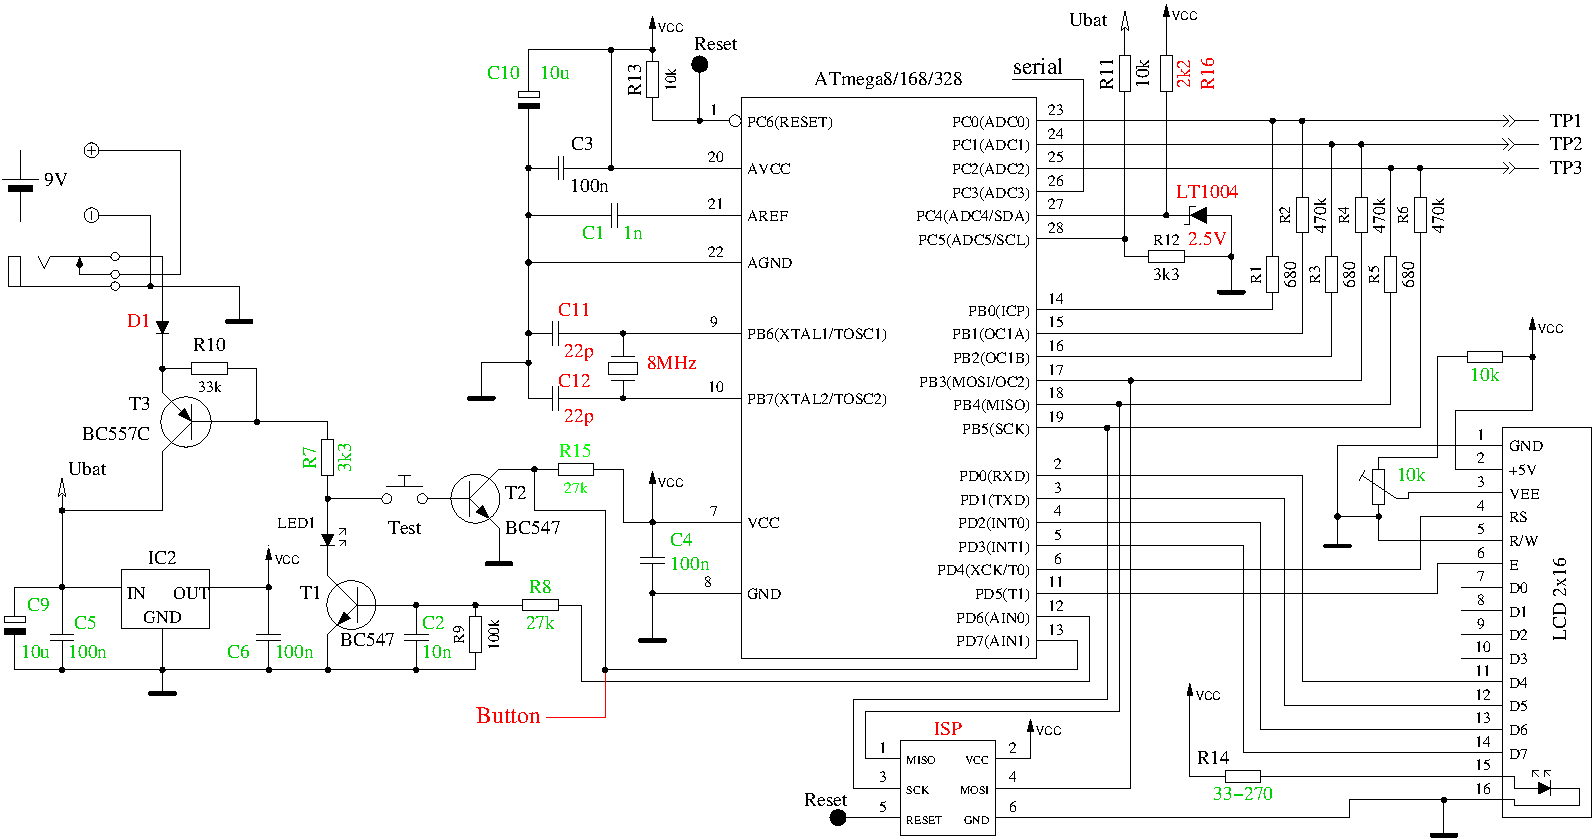
\includegraphics[width=1.0\textwidth]{../FIG/ttester.pdf}
\caption{Neue TransistorTester-Schaltung}
\label{fig:ttester}
\end{figure}

Die Tabelle~\ref{tab:display-con} zeigt die Belegung des PD Ports für verschiedene Display-Versionen
und die Belegung der Zusatzfunktionen.
Bei allen Varianten dieser Tabelle sollten die Zusatzfunktionen möglich sein.
Das Signal LCD-CE bei der SPI Schnittstelle ist am ATmega-Port verfügbar. Der Eingang CE (Chip Enable) des
Controllers kann aber auch fest auf GND gelegt werden anstelle mit dem LCD-CE Ausgang des ATmega verbunden zu werden.

\begin{table}[H] \small
  \begin{center}
    \begin{tabular}{| c || c | c | c | c | c | c |}
    \hline
           & Character     & ST7565 LCD & ST7920 LCD     & NT7108 LCD  & SSD1306     & Zusatzfunktion \\
      Port & LCD           &   SPI      & serial         & serial      &   I\textsuperscript{2}C      & \\
    \hline
    \hline
    PD0    &  LCD-D4       &  LCD-REST  & LCD-REST       & 595-PCLK        &            & \\
    \hline
    PD1    &  LCD-D5       &  LCD-RS    &                & LCD-CS2     &             & Drehgeber-2 \\
    \hline
    PD2    &  LCD-D6       &  LCD-SCLK  & LCD-B0         & 164-595-CLK &  LCD-SDA    & \\
    \hline
    PD3    &  LCD-D7       &  LCD-SI    &                & LCD-CS1     &             & Drehgeber-1 \\
    \hline
    PD4    &  LCD-RS       &            &                & LCD-RS      &             & Frequenzzähler \\
           &               &            &                & 164-595-SER &             &                \\
    \hline
    PD5    &  LCD-E        &  (LCD-CE)  & LCD-EN         & LCD-EN      &   LCD--SCL  & \\
    \hline
    PD7    & Tastensignal & Tastensignal & Tastensignal  & Tastensignal & Tastensignal & \\
    \hline
    \end{tabular}
  \end{center}
  \caption{Pinbelegung für verschiedene Displays}
\label{tab:display-con}
\end{table}

Um einen einfacheren Anschluss des Displays an den ATmega auf Streifenleiterplatinen zu erreichen,
kann die Software auch eine andere Port-D-Belegung berücksichtigen.
Die folgende Tabelle~\ref{tab:grid-change} zeigt die Änderungen der Pinbelegungen für ein Textdisplay und 
alternative Anschlüsse für graphische Displays bei einem ATmega328 Mikrocontroller.
Außerdem werden die Belegungen der Port-Eingänge für zusätzliche Funktionen gezeigt. 
Bei der Belegung für das grafische Display mit der Streifenraster-Option (STRIP\_GRID\_BOARD=1)
kann die Frequenzzähler-Funktion nicht benutzt werden, da diese den Port PD4 (T0) benutzt.
Diese Belegung wird aber von einer chinesischen Version mit graphischem Display benutzt.
In den meisten Fällen sind die Platinenversionen mit einem Textdisplay für die Nachrüstung der
Frequenzzähler Funktion und der Drehgeber Option besser geeignet, weil die erforderlichen
Signale am Displayanschluß zur Verfügung stehen. 


\begin{table}[H]
  \begin{center}
    \begin{tabular}{| c || c | c | c | c |}
    \hline
           & Char. LCD      & ST7565 LCD     & ST7565 LCD   & Zusatzfunktion \\
      Port &    =1          &    =1          &    =5        &  \\
    \hline
    \hline
    PD0    &  Tastensignal  &                &              &  \\
    \hline
    PD1    &  LCD-D7        & LCD-SI         &  LCD-A0 (RS) &  Drehgeber-2 \\
    \hline
    PD2    &  LCD-D6        & LCD-SCLK       &  LCD-REST    &  \\
    \hline
    PD3    &  LCD-D5        & LCD-A0 (RS)    &  LCD-SCLK    &  Drehgeber-1 \\
    \hline
    PD4    &  LCD-D4        & LCD-REST       &  LCD-SI      &  Frequenzzähler \\
    \hline
    PD5    &  LCD-E         & (LCD-CE)       &              &  \\
    \hline
    PD7    & LCD-RS         & Tastensignal   & Tastensignal &  \\
    \hline
    \end{tabular}
  \end{center}
  \caption{Alternative Pinbelegungen mit der Option STRIP\_GRID\_BOARD}
\label{tab:grid-change}
\end{table}

\section{Erweiterungen für den TransistorTester}


\subsection{Schutz der ATmega-Eingänge}  

Zum besseren Schutz der ATmega-Eingänge kann eine Erweiterung mit einem Relais oder mit Dioden
nach Schaltbild~\ref{fig:relay_addon} angeschlossen werden.
Die Ruhekontakte des Relais schützen den ATmega im spannungslosen Zustand.
Die Konkakte werden von der Software nur für die Messung freigegeben.
Auch der Einbau von einem Überspannungsschutz mit Dioden verbessert die Chancen des ATmega
den Anschluss eines Kondensators mit höherer Restspannung zu überleben.
Ein vollständiger Schutz ist aber nicht möglich. Deshalb sollten Kondensatoren vor dem Messen immer
entladen werden.

\begin{figure}[H]
  \begin{subfigure}[b]{.5\textwidth}	%9cm
   \centering
   \begin{overpic}[width=.78\textwidth]{../FIG/relay_addon.pdf}	% width=7cm
    \color{black}
    \put(78,36){\makebox(0,0)[lb]{\footnotesize {VCC oder Ubat}}}  
    \put(78,31){\makebox(0,0)[lb]{\footnotesize {abhängig von Relaisspannung}}}  
   \end{overpic}
  \caption{mit Relais}
  \end{subfigure}
~
  \begin{subfigure}[b]{.5\textwidth}	%9cm
    \centering
    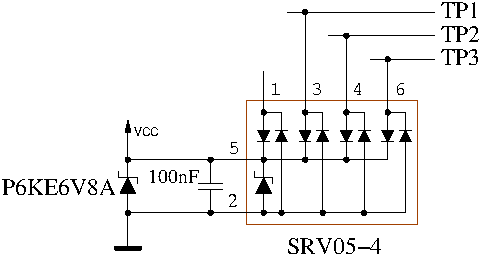
\includegraphics[width=.78\textwidth]{../FIG/diode_addon.pdf}	% width=7cm
    \caption{mit Dioden}
  \end{subfigure}
  \caption{Zusätzlicher Schutz der ATmega-Eingänge}
\label{fig:relay_addon}
\end{figure}

Ein noch besserer Schutz ist mit einem Relais mit 3 Umschaltkontakten nach Abbildung~\ref{fig:relay_um_addon} möglich.
Der Entladestrom wird hier durch Widerstände begrenzt und die ATmega-Eingänge sind im geschützten Zustand getrennt.
Man darf aber nicht vergessen, daß der Tester während der Messung trotzdem ungeschützt bleibt.

\begin{figure}[H]
 \centering
  \begin{overpic}[width=.58\textwidth]{../FIG/relay_um_addon.pdf}	% width=10cm
  \color{black}
  \put(78,42){\makebox(0,0)[lb]{\footnotesize VCC oder Ubat abhängig}}
  \put(78,38){\makebox(0,0)[lb]{{\footnotesize von Relaisspannung}}}
 \end{overpic}
 \caption{Verbesserter Schutz mit Relais}
\label{fig:relay_um_addon}
\end{figure}

\subsection{Zenerspannungsmessung}

Wenn die Ausgabe der seriellen Texte nicht gebraucht wird, kann der Pin PC3 des ATmega für die Messung
einer externen Spannung benutzt werden. Die Spannung kann mit dem optionalen 10:1-Widerstandsteiler
bis zu \(50V\) betragen und kann für die Messung der Zenerspannung einer Diode benutzt werden.
Ein Strombegrenzendes Netzteil mit bis zu \(50V\) Ausgangsspannung kann mit dem \(0V\)-Signal des ATmega PD7-Pins
eingeschaltet werden, um zum Beispiel die Durchbruchspannung von Zenerdioden zu messen.
Einen Vorschlag für diese Erweiterung zeigt Abbildung~\ref{fig:zener}.
Der Tester zeigt die externe Spannung so lange an, wie man den Taster gedrückt läßt.
Ungefähr \(40mA\) mehr Batteriestrom wird für diese Erweiterung bei gedrückter Taste gebraucht.

\begin{figure}[H]
 \centering
 \begin{overpic}[width=.90\textwidth]{../FIG/zener_exp.pdf}	% width=15.5cm
  \color{black}
% \put(42,25){\makebox(0,0)[cb]{Taster}}       % Button ist Signalname in der Basis-Zeichnung!
  \put(5,20){\makebox(0,0)[rb]{\textcolor{red}{externe}}}  
  \put(5,17){\makebox(0,0)[rb]{\textcolor{red}{Spannung}}}  
  \put(33,24){\makebox(0,0)[rb]{Hat Platz auf der Platine!}} 
  \put(42,2){\makebox(0,0)[lb]{Sollte separat positioniert werden!}}    
 \end{overpic}
 \caption{Erweiterung zum Messen von Zenerspannungen}
\label{fig:zener}
\end{figure}

Der 10:1-Spannungsteiler kann mit dem optionalen Dialogteil für den ATmega328 auch ohne 
den Spannungswandler benutzt werden. Ohne die gedrückte Taste ist der Spannungswandler nicht in 
Betrieb, sodass eine externe Spannung (z.B. Batteriespannung) am Zenerdioden-Port gemessen werden kann.
Es können nur positive Gleichspannungen bis \(50V\) gemessen werden.
Man muss also auf die richtige Polarität achten.

\subsection{Frequenzgenerator}

Mit dem Dialogteil des ATmega kann außerdem ein Frequenzgenerator angewählt werden, der derzeit
Frequenzen von \(2MHz\) bis \(1Hz\) ausgeben kann. Der Ausgang des \(5V\)-Signals erfolgt über
einen \(680\Omega\)-Widerstand auf den Testport TP2. Als Massesignal kann der Minus-Anschluss
der Zenerdiodenerweiterung oder Anschluss TP1 benutzt werden.
Auch TP3 ist über den \(680\Omega\) Widerstand mit Masse verbunden.
Natürlich kann an den ATmega-Port PB2 auch eine Schaltung zum Verstärken des Ausgangssignals 
für einen getrennten Ausgang angeschlossen werden. Dabei sollte der Eingang dieser Schaltung
aber keine hohe kapazitive Last für den ATmega-Ausgang darstellen.

\subsection{Frequenzzähler}
\label{sec:frequency_counter}
Für die ebenfalls über die Dialogfunktion wählbare Frequenz-Messung ist eine kleine Erweiterung
der Schaltung erforderlich. Als Eingang für die Frequenzmessung wird der PD4-Pin (T0/PCINT20) des
ATmega benutzt. Der gleiche Pin wird auch zum Anschluss des LCD benutzt. Bei dem normalen Layout
ist dies LCD-RS, beim Streifenraster-Layout ist dies LCD-D4. Für beide Signale kann der PD4-Pin
auf Eingang geschaltet werden und für die Messung benutzt werden, solange keine Ausgabe auf das
LCD erfolgt. Das LCD interessiert sich für das Signal nur, wenn LCD-E auf GND geschaltet wird.
Für die Einspeisung des Testsignals ist mindestens ein Serienwiderstand von \(270\Omega\) erforderlich.
Besser ist eine Schaltung nach Abbildung~\ref{fig:FreqMes} zu benutzen. Die Spannung am PD4-Pin (LCD-RS oder
LCD-D4) sollte ohne eingesteckten ATmega oder im Frequenz-Messbetrieb auf etwa \(2,4V\) eingestellt sein,
damit die größte Empfindlichkeit für das Eingangssignal erzielt wird. Das LCD sollte aber eingesteckt sein,
weil dessen Pull-Up Widerstände die Spannung verändern.

\begin{figure}[H]
\centering
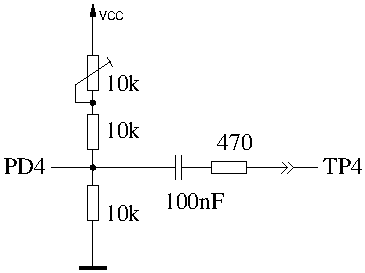
\includegraphics[width=.4\textwidth]{../FIG/Frequency_addon.pdf}	% width=7cm
\caption{Erweiterung zum Messen von Frequenzen}
\label{fig:FreqMes}
\end{figure}

\subsection{Impulsdrehgeber}
\begin{wrapfigure}{r}{0.3\textwidth}
\vspace{-4\baselineskip}
\begin{center}
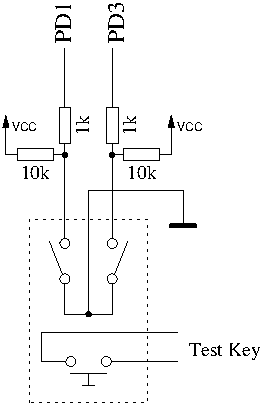
\includegraphics[width=0.2\textwidth]{../FIG/rotary_extension.pdf}
\put(-40,33){\makebox(0,0)[lb]{Taster}} 
\end{center}
\vspace{-0.7\baselineskip}
 \caption{\\Impulsdrehgeber-Erweiterung}
\vspace{-2\baselineskip}
\label{fig:RotExt}
\end{wrapfigure}
Zur leichteren Bedienung der Menüfunktion für den ATmega328 kann die Schaltung um einen
Impulsdrehgeber mit Taster erweitert werden.
Die Schaltung~\ref{fig:RotExt} gibt die Standard-Belegung
für ein normales LCD an. Alle Anschlüsse für den Impulsdrehgeber sind an der Steckerleiste für das LCD 
verfügbar. 
Deswegen kann der Impulsdrehgeber in vielen Fällen leicht nachgerüstet werden. 
Vielfach ist das graphische Display auch mit einem Adapter-Board an die Steckerleiste des LCD angeschlossen. 
Deswegen ist auch hier die Nachrüstung des Impulsdrehgebers nicht sehr schwierig.\\
\clearpage
\begin{figure}[t]
 \centering
 \begin{overpic}[width=.8\textwidth]{../FIG/rotary_encoder.pdf}	% width=15cm
  \color{black}
  \put(90,71.7){\makebox(0,0)[lb]{Schalter A}}
  \put(90,62){\makebox(0,0)[lb]{Schalter B}}
  \put(90,29){\makebox(0,0)[lb]{Schalter A}}
  \put(90,19){\makebox(0,0)[lb]{Schalter B}}
  \put(6,6){\makebox(0,0)[rb]{\footnotesize{Zustand:}}}
  \put(6,48.5){\makebox(0,0)[rb]{\footnotesize{Zustand:}}}
  \multiput(23.5,53) (24.6,0){3}{\footnotesize {Rastung}}
  \multiput(11,10) (12.3,0){6}{\footnotesize {Rastung}}
  \put(52,43){\makebox(0,0)[cb]{\large{Version 2}}}
  \put(52,1){\makebox(0,0)[cb]{\large{Version 1}}}
 \end{overpic}
 \caption{Zwei unterschiedliche Versionen eines Impulsdrehgeber}
\label{fig:RotEnc}
\end{figure}

Die Abbildung~\ref{fig:RotEnc} zeigt zwei Versionen von Drehgebern. Die Version 1 hat doppelt so viele Raststellungen (detent) pro Umdrehung wie Pulse pro Umdrehung.
Die Version 2 hat gleich viele Pulse pro Umdrehung wie Raststellungen.
Manchmal liegt bei einigen Drehgebern die Schaltflanke eines der beiden Schalter genau an der
Raststellung.

\begin{figure}[H]
 \centering
 \begin{overpic}[width=.87\textwidth]{../FIG/rotary_bouncing.pdf}	% width=17cm
  \color{black}
  \put(90,39){\makebox(0,0)[lb]{Schalter A}}
  \put(90,30){\makebox(0,0)[lb]{Schalter B}}
  \multiput(11,23) (28,0){3}{\footnotesize {Rastung}}
  \put(7,20){\makebox(0,0)[rb]{Zustand}}
  \put(5,12){\makebox(0,0)[lb]{Mögliche Zustände von links nach rechts:}}
 \end{overpic}
 \caption{Ein Impulsdrehgeber mit prellenden Kontakten}
\label{fig:RotBounce}
\end{figure}

Die Abbildung~\ref{fig:RotBounce} zeigt einen Impulsdrehgeber, der nicht nur
prellende Kontakte hat, sondern auch an den Raststellungen (detent) einen unsicheren Zustand
eines der Kontakte besitzt. Jeder Wechsel eines Schalterzustandes wird vom Programm 
überwacht und in einem zyklischen Puffer gespeichert. Damit kann bei einem Wechsel des
Zustandes auch die beiden vorigen Zustände geprüft werden.
Insgesamt können für einen Zyklus der Schaltzustände vier Zustandsfolgen für jede Drehrichtung
festgelegt werden. Wenn nur eine Raststellung pro Zyklus vorhanden ist, reicht die Abfrage eines
Paares dieser Zustandsfolgen für das Zählen der Raststellung in beide Richtungen aus (WITH\_ROTARY\_SWITCH=2 oder 3).
Bei zwei Raststellungen, wie in der Abbildung~\ref{fig:RotBounce} gezeigt ist,
müssen zwei Paare abgefragt werden (WITH\_ROTARY\_SWITCH=1).
Für Impulsdrehgeber ohne Rasterung kann die Einstellung für WITH\_ROTARY\_SWITCH beliebig auf
2 oder 3 für die niedrigste Empfindlichkeit, auf 1 für eine mittlere Empfindlichkeit und auf 5 für
die höchste Empfindlichkeit gesetzt werden. 
Ein Pendeln der Einstellung (Zähler rauf, Zähler runter) wird durch die Art der Abfrage vermieden, bei
ungünstiger Lage der Schaltflanken kann aber ein Zählpuls für eine Raststellung ausbleiben.



Anstelle der beiden Kontakte für den Impulsdrehgeber können auch zwei Taster für Rauf (Up) und Runter (Down)
eingebaut werden, wenn kein Impulsdrehgeber vorhanden oder gewünscht ist.
Für diesen Fall muss die Option WITH\_ROTARY\_SWITCH auf 4 gesetzt werden, damit das Programm
entsprechend reagiert.

\subsection{Anschluss eines graphischen Displays}

Dank der Arbeit von Wolfgang Sch. für die Unterstützung der chinesischen Version mit
grafischem 128x64 Pixel LCD, kann mittlerweile auch ein grafisches LCD
mit ST7565-Controller angeschlossen werden. Da der ST7565-Controller seriell angesteuert wird,
werden nur vier Signalleitungen benötigt.
Dadurch werden zwei Pinne des Port D für andere Verwendung frei.
Der ATmega-Prozessor sollte mindestens 32k Flash-Speicher besitzen.
Der ST7565-Controller wird mit einer Betriebsspannung von \(3,3V\) betrieben.
Deswegen ist ein zusätzlicher Spannungsregler notwendig.
Nach dem Controller Datenblatt dürfen keine \(5V\) Signale direkt mit den Controller-Eingängen verbunden
werden. Deshalb ist in der Erweiterung nach Bild~\ref{fig:ST7565lcd} ein zusätzlicher CMOS 74HC4050
für die Pegelanpassung vorgesehen. 
Man kann auch versuchen, die vier Gatter des 74HC4050 durch vier Widerstände von etwa \(2,7k\Omega\) zu ersetzen.
Über den Spannungsabfall an den Widerständen wird verhindert, dass die \(3,3V\)-Versorgung des Controllers über die Schutzdioden
der Controllereingänge von den \(5V\) ATmega-Ausgängen über die \(3,3V\)-Grenze angehoben werden kann.
Ob die Signalform für den ST7565-Controller so noch akzeptiert wird, sollte man vorher testen.
Mit den Gattern des 74HC4050 bleibt die Signalform jedenfalls besser erhalten.\\
 
\begin{figure}[H]
 \centering
 \begin{overpic}[width=.814\textwidth]{../FIG/ST7565lcd.pdf}	% width=14cm
  \color{black}
  \put(88,10){\makebox(0,0)[lb]{Hintergrund}}
  \put(88,7){\makebox(0,0)[lb]{LED}}
 \end{overpic}
 \caption{Anschluss eines graphischen Displays mit ST7565 Controller}
\label{fig:ST7565lcd}
\end{figure}

Die Tabelle~\ref{tab:spi-processor} zeigt weitere Anschlußmöglichkeiten
für den ATmega328 und andere Prozessoren mit der SPI (LCD\_INTERFACE\_MODE=4)
oder der 3LINE (LCD\_INTERFACE\_MODE=3) Schnittstelle. \\
Verschiedene Belegungen für
einen Prozessor werden mit der Makefile Option STRIP\_GRID\_BOARD
eingestellt.
Die Belegungen sind in der Datei config.h festgelegt. 
Wenn weitere Varianten der Belegung erforderlich sind, sollten diese
mit weiteren Kennziffern der Option STRIP\_GRID\_BOARD auswählbar sein
und in config.h ergänzt werden.

\begin{table}[H]
  \begin{center}
    \begin{tabular}{| c || c | c | c | c | c | c | c |}
    \hline
 Processor  & m644  & m1280 & m1280  & m328 & m328 & m328 & m328 \\
STRIP\_GRID\_BOARD &       &   -   &   1    &  -   &  1   &  2   &  5   \\
    \hline
    \hline
Signal:     &       &       &        &      &      &      &      \\
  RES       &  PB4  & PA0   &  PA4   & PD0  & PD4  & PD0  & PD2 \\
    \hline
  EN, CLK   &  PB6  & PA2   &  PA2   & PD2  & PD2  & PD2  & PD3 \\
    \hline
  RS, D/C   &  PB5  & PA1   &  PA3   & PD1  & PD3  & PD3  & PD1 \\
    \hline
  B0, MOSI  &  PB7  & PA3   &  PA1   & PD3  & PD1  & PD1  & PD4 \\
    \hline
  CE, CS    &  PB3  & PA4   &  PA5   & PD5  & PD5  & PD5  & PD5 \\
    \hline
    \end{tabular}
  \end{center}
  \caption{SPI Anschlußbelegungen für verschiedene Prozessoren}
\label{tab:spi-processor}
\end{table}

Normalerweise wird der ST7565- oder der SSD1306-Controller mit einer 4-Wire SPI-Schnittstelle angeschlossen.
Beim SSD1306-Controller kann auch eine I\textsuperscript{2}C-Schnittstelle mit PD2 als SDA- und PD5 als SCL-Signal benutzt werden.
Die SDA- und SCL-Signale müssen mit einem \inquotes{Pull-up} Widerstand von ungefähr \(4,7k\Omega\) nach \(3,3V\) versehen sein.
Eine Anschlußmöglichkeit zeigt die Abbildung~\ref{fig:ssd1306i2c}.
Vor der Verwendung der \inquotes{Pull-up} Widerstände nach \(5V\) sollte überprüft werden, ob die Eingänge dieses Signal vertragen.
Normalerweise sind die Eingänge des Kontrollers über Dioden nach \(3.3V\) geschützt.
Die Ausgänge des ATmega werden für die I\textsuperscript{2}C-Signale nur nach \(0V\) geschaltet.
Es sollte aber sichergestellt sein, daß das Programm mit der I\textsuperscript{2}C Schnittstelle in den ATmega geladen wurde,
bevor das Display angeschlossen wird. Wenn ein Programm für eine andere Schnittstelle geladen wurde,
werden die Ausgänge auch nach \(5V\) geschaltet.
Da ich eine Beeinflussung der Meßergebnisse der Testers über den VCC-Anschluß der OLED-Module festgestellt habe, 
ist eine Entkopplung über einen Serienwiderstand von \(68\Omega\) mit zusätzlichem \(10\mu F\)
 Abblock-Kondensator zu empfehlen. 
Anstelle des \(68\Omega\) Widerstand kann auch eine Drossel von etwa \(1mH\) verwendet werden.
Ohne das zusätzliche Filter wurde bei meinem Tester Kollektorrestströme bei bipolaren Transistoren mit einem OLED angezeigt.
Außerdem sollte die Belegung der Pinne beim OLED Modul geprüft werden, bei einigen Modulen ist GND und VCC vertauscht!
 
\begin{figure}[H]
\centering
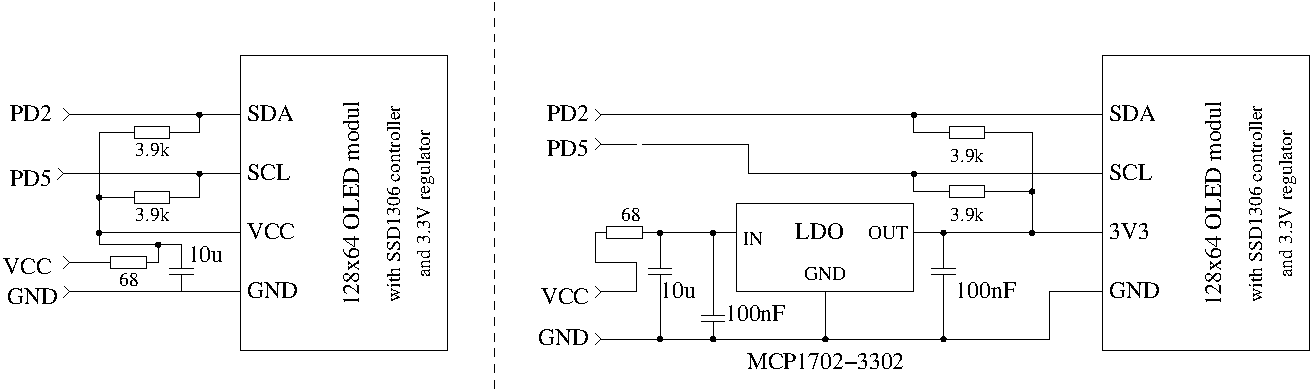
\includegraphics[width=.814\textwidth]{../FIG/SSD1306_I2C.pdf}	% width=17cm
\caption{Anschluss eines graphischen OLED Displays mit I\textsuperscript{2}C Schnittstelle}
\label{fig:ssd1306i2c}
\end{figure}

Bei der ATmega644 Prozessorserie werden die Pinne PB3 (SCL) und PB4 (SDA) anstelle PD5 und PD2 für den Anschluss benutzt.
Bei der ATmega1280 Prozessorserie werden die Pinne PA5 (SCL) und PA4 (SDA) benutzt.
Ein Austausch des Textdisplays gegen ein grafisches Display ist mit einer Adapterplatine möglich, da
alle notwendigen Datensignale und Versorgungssignale an der LCD-Steckerleiste vorhanden sind.
Etwas einfacher ist der Anschluß eines graphischen Displays mit einem ST7920 Controller weil 
der Controller mit \(5V\) Betriebsspannung läuft.
Dabei sollte das Display 128x64 sichtbare Pixel besitzen.
Das Display Modul mit dem ST7920 Controller kann entweder mit der 4-Bit Parallelschnittstelle oder mit einer 
speziellen Seriellschnittstelle angeschlossen werden, wie die Abbildung~\ref{fig:ST7920lcd} zeigt.
 
\begin{figure}[H]
 \centering
 \begin{overpic}[width=.698\textwidth]{../FIG/ST7920interface.pdf}	% width=12cm
  \color{black}
  \put(20,1){\makebox(0,0)[cb]{seriell Betrieb}}
  \put(80,1){\makebox(0,0)[cb]{4-bit parallel Betrieb}}
 \end{overpic}
 \caption{Anschluss eines Displays mit ST7920 Controller}
\label{fig:ST7920lcd}
\end{figure}

Für beide Anschlußarten muß die Software speziell konfiguriert werden. 
Die Makefile Option \inquotes{WITH\_""LCD\_""ST7565 = 7920} muß dazu auf jeden Fall gesetzt werden, für die serielle
Anschlußart muß außerdem die Option \inquotes{CFLAGS += -DLCD\_""INTERFACE\_""MODE=5} gesetzt sein.
Die Tabelle~\ref{tab:ser-processor} zeigt die Belegung der seriellen Anschlußsignale bei 
dem Anschlußtyp 5 (ST7920) und 7 (SSD1803) für verschiedene Prozessoren.

\begin{table}[H]
  \begin{center}
    \begin{tabular}{| c || c | c | c | c |}
    \hline
 Processor  & m644  & m644 & m1280  & m328 \\
STRIP\_GRID\_BOARD &       &   1   &        &     \\
    \hline
    \hline
Signal:     &       &       &        &         \\
  EN        &  PB3  & PB6   &  PA5   & PD5     \\
    \hline
  B0, R/W   &  PB4  & PB7   &  PA4   & PD2      \\
    \hline
  RESET     &  PB2  & PB4   &  PA0   & PD0      \\
    \hline
    \end{tabular}
  \end{center}
  \caption{Serielle Anschlußbelegungen für verschiedene Prozessoren}
\label{tab:ser-processor}
\end{table}

Die Ausrichtung der Darstellung kann wie bei allen graphischen Displays  mit den Optionen
LCD\_ST7565\-\_H\_FLIP und LCD\_ST7565\-\_V\_FLIP angepaßt werden. \\

Einen Sonderfall stellen Displays mit NT7108 oder KS0108 (S6B0108) Controller dar. Da die Displays nur mit 8-Bit Parallelschnittstelle
angesteuert werden können, ist ein externer seriell-parallel Wandler erforderlich.
Die einfachste Lösung scheint mir mit einem 74HCT164 oder einem 74HCT595 Chip möglich zu sein.
Einen entsprechenden Schaltungsvorschlag zeigt das Bild~\ref{fig:NT7108lcd}.

\begin{figure}[H]
  \begin{subfigure}[b]{.5\textwidth}	% 9cm
    \centering
    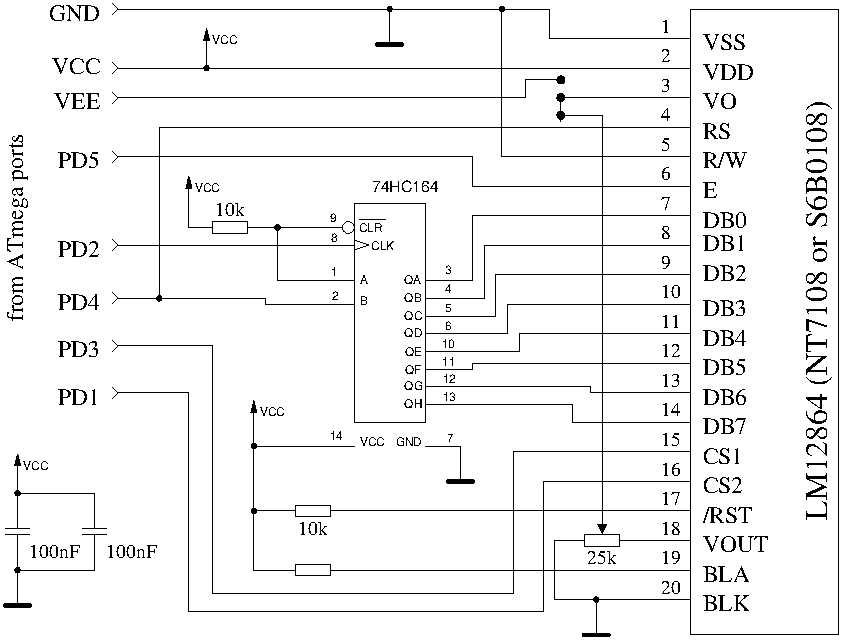
\includegraphics[width=.9\textwidth]{../FIG/ST7108serial164.pdf}	% 8cm
    \caption{mit 74HCT164}
  \end{subfigure}
~
  \begin{subfigure}[b]{.5\textwidth}	% 9cm
    \centering
    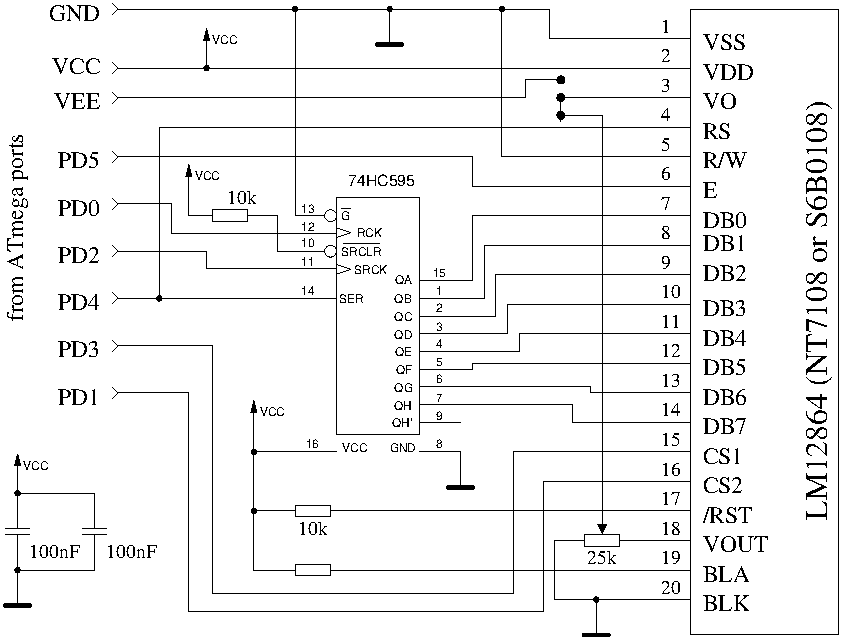
\includegraphics[width=.9\textwidth]{../FIG/ST7108serial595.pdf}	% 8cm
    \caption{mit 74HCT595}
  \end{subfigure}
  \caption{Anschluss eines graphischen Displays mit NT7108 Controller}
\label{fig:NT7108lcd}
\end{figure}

Sie müssen die Pinreihenfolge bei Ihrem LCD-Modul prüfen, einige Module haben eine andere Signalreihenfolge.

Einige verschiedene Pinbelegungen aus Datenblättern der ABG128064 Serie zeigt Tabelle~\ref{tab:NT7108types}.

\begin{table}[H]
  \begin{center}
    \begin{tabular}{| c || c | c | c | c |}
    \hline
           & 128064H  &  128064G  & 128064C  & 128064B \\
    Signal &         &          &         &         \\
    \hline
    \hline
  VDD (5V) &   1     &  2       &   4     & 2       \\
    \hline
  VSS (GND) &   2     &  1       &   3     & 1       \\
    \hline
 VO (Drive) &   3     &  3       &  (5)    & 3       \\
    \hline
  DB0-DB3   &   4-7   &  7-10    &   9-12  & 7-10    \\
    \hline
  DB4-DB7   &   8-11  &  11-14   &   13-16 & 11-14   \\
    \hline
  CS1       &   12    &  15      &   1     & 15      \\
  CS2       &   13    &  16      &   2     & 16      \\
    \hline
  Reset     &   14    &  17      &   -     & 17      \\
    \hline
  R/W       &   15    &  5       &   7     & 5       \\
    \hline
  RS        &   16    &  4       &   6     & 4       \\
    \hline
  E         &   17    &  6       &   8     & 6       \\
    \hline
  VEE       &   18    &  18      &   -     & 18      \\
    \hline
  LEDA      &   19    &  19      &   17    & (19)      \\
  LEDK      &   20    &  20      &   18    & -      \\
    \hline
    \end{tabular}
  \end{center}
  \caption{Pinbelegung verschiedener NT7108 Module}
\label{tab:NT7108types}
\end{table}

Die Tabelle~\ref{tab:7108-processor} zeigt die Belegung des seriellen NT7108 Controller
Anschluß für verschiedene Prozessor-Serien.
\begin{table}[H]
  \begin{center}
    \begin{tabular}{| c || c | c | c |}
    \hline
 Processor  & m644  &  m1280  & m328 \\
    \hline
    \hline
Signal:     &       &        &         \\
  EN        &  PB3  &  PA5   & PD5     \\
    \hline
  RS        &  PB2  &  PA4   & PD4      \\
  B0        &  PB2  &  PA4   & PD4      \\
    \hline
  CS1       &  PB7  &  PA3   & PD3      \\
    \hline
  CS2       &  PB5  &  PA1   & PD1      \\
    \hline
  CLK       &  PB6  &  PA2   & PD2      \\
    \hline
  PCLK      &  PB4  &  PA0   & PD0      \\
    \hline
    \end{tabular}
  \end{center}
  \caption{Serieller NT7108 Anschluß für verschiedene Prozessoren}
\label{tab:7108-processor}
\end{table}

Es können auch Displays mit einem PCF8814 Controller verwendet werden, wie sie beispielsweise
in einem Nokia 1100 Handy verbaut sind. Hierbei ist zu prüfen, welches Interface von dem Display-Modul
verwendet wird. Der PCF8814 Controller unterstützt die SPI-Schnittstelle als 3-line und 4-line,
die I\textsuperscript{2}C-Schnittstelle und eine spezielle 3-line Schnittstelle, bei der das
Daten/Instruktion - Signal als erstes serielles Bit übertragen wird.
Das Display besitzt nur 96x65 Pixel, daher werden keine großen graphischen Symbole für die
Transistoren bei diesem Controller benutzt. Die Ausgabe is also ähnlich wie auf einem Textdisplay.
Wie bei den meisten graphischen Displays ist auch hier die Betriebsspannung 3.3 Volt.
Deswegen ist eine Signalanpassung an die \(5V\) Ausgänge des ATmega erforderlich.
Für die SPI-Schnittstelle und die 3-line Schnittstelle können die Ausgänge des ATmega
mit der Makefile Option LCD\_SPI\_OPEN\_COL wie ein \inquotes{Open Collector} Ausgang benutzt werden.
Es sind aber \inquotes{Pull-Up} Widerstände erforderlich oder es darf die Option PULLUP\_DISABLE
in der Makefile nicht gesetzt sein.
Getestet ist derzeit nur die 3-line Schnittstelle.

\begin{table}[H]
  \begin{center}
    \begin{tabular}{| c || c | c | c | c |}
    \hline
           &  PCF8814    & PCF8814        & PCF8814     & Zusatzfunktion \\
      Port &    SPI      & 3-line         &   I\textsuperscript{2}C      & \\
    \hline
    \hline
    PD0    &   LCD-REST  & LCD-REST       &            & \\
    \hline
    PD1    &   LCD-D/C   & LCD-SCE        &             & Drehgeber-2 \\
    \hline
    PD2    &   LCD-SCLK  & LCD-SCLK       &  LCD-SDIN   & \\
    \hline
    PD3    &   LCD-SDIN  & LCD-SDIN       &             & Drehgeber-1 \\
    \hline
    PD4    &             &                &             & Frequenzzähler \\
    \hline
    PD5    &             & LCD-EN         &   LCD-SCLK  & \\
    \hline
    \end{tabular}
  \end{center}
  \caption{Pinbelegung für verschiedene Anschlussvarianten des PCF8814 Kontrollers}
\label{tab:PCF8814-con}
\end{table}

Es ist auch eine Unterstützung für einen PCF8812 controller mit 102x65 Pixeln bereits vorhanden,
aber völlig ungetestet.

\subsection{Anschluss eines graphischen Farbdisplays}

Von chinesischen Händlern werden preisgünstige Farbdisplay-Module mit einer SPI Schnittstelle angeboten.
Die Abbildung~\ref{fig:Color_both} zeigt die Rückseite der beiden unterstützten Module mit 128x128 Pixeln
und 128x160 Pixeln.
Diese Module sind sehr klein, so werden auch Texte und Symbole sehr klein dargestellt.
Aber das Erscheinungsbild ist scharf und klar.

\begin{figure}[H]
\centering
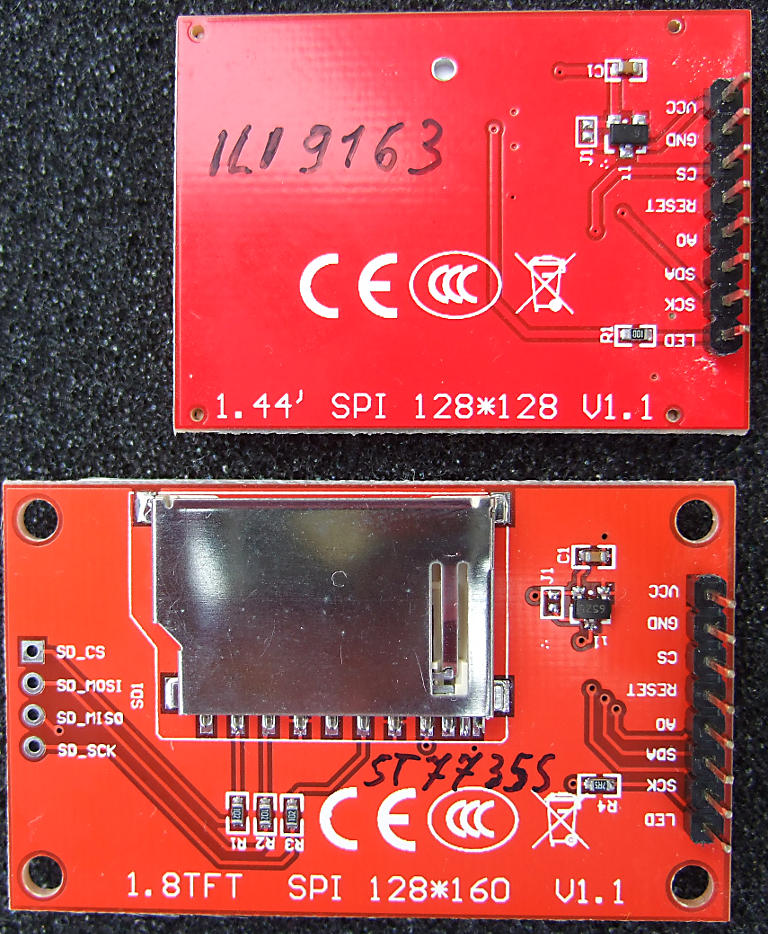
\includegraphics[width=.46\textwidth]{../PNG/Color_ILI9163_ST7735.jpg}	% width=8cm
\caption{Rückseite der beiden Color-LCD's}
\label{fig:Color_both}
\end{figure}

Das 128x128 Pixel Modul benutzt einen ILI9163 Kontroller.
Das 128x160 Pixel Modul benutzt einen sehr ähnlichen ST7735 Kontroller.
Getestet habe ich die Module mit einem Adapterboard, der die Verbindungen
der SPI-Signale und der Stromversorgung zu der Anschlußleiste des normalen Textdisplays
herstellt. Die Anpassung der \(5V\) Signale des ATmega an die \(3.3V\) Eingänge des Kontrollers
habe ich mit seriellen \(10k\Omega\) Widerständen vorgenommen.
Die Hintergrundbeleuchtung (LED) ist für diese Module unbedingt erforderlich, da sonst
nichts erkennbar ist.
Aufgrund der hohen Pixelzahl in vertikaler Richtung können auf den Displays mehr Textzeilen dargestellt
werden. Für das 128x128 Pixel Display können bis zu 8 Textzeilen mit einem 12x8 Font dargestellt werden,
Für das 128x160 Pixel Display sind es sogar 10 Textzeilen.
Auf dem Foto~\ref{fig:Color_PNP} ist das Ergebnis einer Messung eines Germanium Transistors auf einem
128x128 Pixel Display zu sehen.

\begin{figure}[H]
\centering
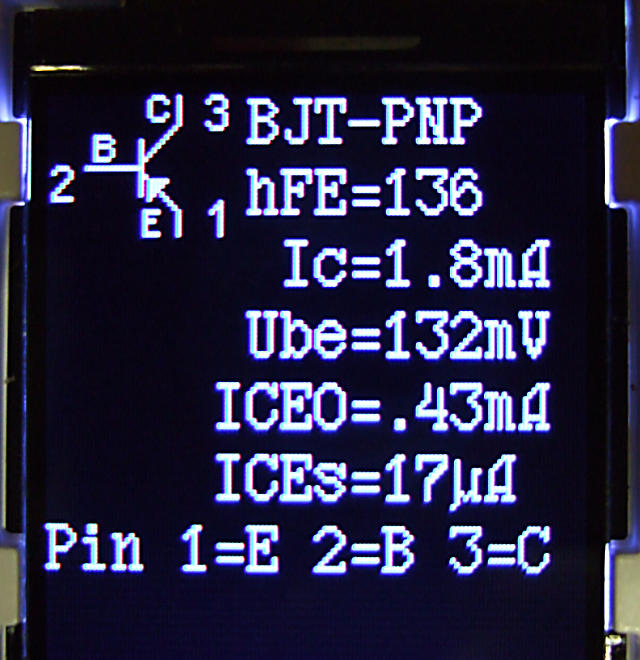
\includegraphics[width=.46\textwidth]{../PNG/Color_PNP_ILI9163.jpg}	% width=8cm
\caption{Messung eines bipolaren PNP Transistors}
\label{fig:Color_PNP}
\end{figure}

Die Farbmöglichkeiten der Displays werden derzeit nicht genutzt. Lediglich die Hintergrundfarbe
und die Vordergrundfarbe könnten in der Datei lcd\_defines.h oder in der Makefile verändert werden.
Es wird das 16-Bit Farbmodell der Kontroller benutzt, die Vordergrundfarbe kann mit der Konstanten
LCD\_FG\_COLOR und die Hintergrundfarbe mit der Konstanten LCD\_BG\_COLOR eingestellt werden.

\section{Hinweise für den Aufbau des TransistorTesters}
Jede LCD-Anzeige-Einheit mit mindestens 2x16 Zeichen und einem HD44780-kompatiblen Controller kann mit
dem TransistorTester benutzt werden.
Man sollte auf den Strombedarf der Hintergrundbeleuchtung achten, einige Anzeigen benötigen
mehr Strom als andere.
Ich habe OLED-Anzeigen ausprobiert, aber diese Anzeigen haben teilweise die Messung des
ATmega beeinflusst und werden nicht empfohlen. Auch das Laden der Spezialzeichen für die 
Widerstandsdarstellung hat mit OLED's Schwierigkeiten ergeben.

Die Widerstände R1 bis R6 sind kritisch für die Messungen und diese \(680\Omega\) und
\(470k\Omega\) Widerstände sollten Messwiderstände sein (Toleranz von \(0,1\%\)), um 
die volle Genauigkeit zu erreichen.
Man sollte Präzisions-Sockel für den ATmega-Mikrocontroller verwenden, um
die Austauschbarkeit des Mikrocontrollers sicherzustellen.
Es kann ein ATmega8, ATmega168 und ATmega328 Mikrocontroller verwendet werden.
Empfohlen wird ein ATmega328, wenn man alle Funktionen nutzen möchte.

Jedenfalls sollte man zuerst alle Bauteile ohne den Mikrocontroller bestücken.
Es wird als IC2 ein moderner \inquotes{low voltage drop}-Spannungsregler wie MCP1702-5002 empfohlen, weil
dieser nur \(2\mu A\) Ruhestrom benötigt und auch noch \(5V\) liefern kann, 
 wenn die Eingangsspannung nur \(5,4V\) beträgt.
Aber dieser Regler ist leider nicht Pin-kompatibel zum bekannteren 78L05-Regler im TO-92-Gehäuse!

Nachdem alle benötigten Bauteile bestückt sind, sollte zuerst die Batterie
oder das Netzteil angeschlossen werden. Das LCD sollte dabei nicht angeschlossen sein, und der Mikrocontroller sich noch nicht im Sockel befinden.
Man sollte die Betriebsspannung des Mikrocontrollers und der LCD-Anzeige
überprüfen während der Start-Taster gedrückt wird.
Die Betriebsspannung sollte verschwinden, wenn man den Start-Taster loslässt.
Wenn die Betriebsspannung die richtige Polarität und Grösse hatte,
sollte man die Strom-Versorgung entfernen und den Mikrocontroller 
richtig herum einstecken. Seien Sie bitte vorsichtig und stellen Sie sicher,
dass alle Pinne des Mikrocontrollers im Sockel stecken.
Danach können Sie das LCD anschliessen. Prüfen Sie, dass die GND- und VCC-Anschlüsse des LCD richtig mit der Baugruppe verbunden sind.

Wenn Sie sicher sind, dass alles richtig angeschlossen ist, schliessen Sie
die Spannungsversorgung wieder an.
Wenn Sie den ATmega schon programmiert haben, können Sie den Start-Taster
drücken.
Durch das Drücken des Start-Tasters sollte die Hintergrundbeleuchtung
der LCD-Anzeige angehen.
Wenn Sie den Taster loslassen, sollte die LED auf der Platine schwach leuchten.
Beachte, dass die Software für den Mikrocontroller für den richtigen
Prozessor-Typ übersetzt sein muss. Ein Programm für den ATmega8 läuft
nicht auf einem ATmega168!

\section{Umrüstung von Tester Versionen nach Markus F.}
\label{sec:change_markus}
\begin{description}

\item[Spannungsüberwachung]  
Das Problem zeigt sich durch sofortiges Abschalten beim Einschaltversuch.
Bei den von mir empfohlenen Einstellungen der fuses (Makefile) wird die Spannungsüberwachung der
verschiedenen ATmega-Versionen auf \(4V\) gesetzt (brown out level). Deswegen kann es beim
Einschalten des Testers zu Problemen kommen, weil der Pin PD6 versucht, den \(100nF\)-Kondensator C2
direkt zu schalten. Dabei kann es zu einem unerwünschten \(5V\) Spannungseinbruch kommen.
Der Kondensator C2 kann problemlos auf \textless~\(10nF\) verkleinert werden. Nach Möglichkeit sollte
man statt der direkten Verbindung PD6 zum Kondensator einen Widerstand \textgreater~\(220\Omega\) 
als Verbindung benutzen.
\item[Verbessern des Einschaltverhaltens]
Der Fehler zeigt sich oft, dass der Tester bei gedrücktem Taster zwar einschaltet, aber wieder
abschaltet, wenn der Taster losgelassen wird. Das Problem tritt öfter auf, wenn die Hintergrund-
Beleuchtung des LCD viel Strom braucht.
Der Widerstand R7 zur Basis des PNP-Transistors T3 war mit \(27k\Omega\) sehr auf Stromsparen
optimiert. Der Widerstand sollte besser auf \(3,3k\Omega\) verkleinert werden um auch bei
geringerer Batteriespannung oder bei geringem Stromverstärkungsfaktor des PNP-Transistors T3
ein sicheres Einschalten zu gewährleisten.
\item[Zusätzlicher Pull-Up-Widerstand an PD7]
Der Fehler zeigt sich dadurch, dass der Tester nach einer kurzen Anzeigezeit mit der Meldung
		\inquotes{Timeout} abschaltet. Die Software ist standardmäßig so konfiguriert (Option PULLUP\_DISABLE),
dass die internen Pull-Up-Widerstände abgeschaltet sind.
Dadurch ist der Pegel am Pin PD7 nicht mehr definiert,
wenn er nicht durch den Taster oder T2 auf GND-Potential geschaltet ist. Ein externer
Pull-Up-Widerstand von \(27k\Omega\) nach VCC vermeidet diesen Fehler.
\item[Kondensator C1 am AREF Pin]
In vielen Entwürfen wird hier ein \(100nF\)-Kondensator verwendet, so auch im Entwurf vom Markus Frejek.
Solange die Referenzspannung des ADC nicht verändert wird, ist das auch in Ordnung.
Bei der Software für den Transistortester für den ATmega168/328 wird aber eine automatische
Umschaltung der Referenzspannung von \(5V\) auf die interne Referenzspannung von \(1,1V\) vorgenommen,
wenn die Eingangsspannung unter etwa \(1V\) liegt. Damit wird eine bessere Auflösung erreicht.
Leider erfolgt die Umschaltung von \(5V\) auf die \(1.1V\) sehr langsam, was eine zusätzliche
Wartezeit von \(10ms\) erfordert. Durch den Austausch des \(100nF\) Kondensators gegen einen \(1nF\)
kann die Wartezeit deutlich verringert werden. Einen Einfluß des kleineren Kondensators
auf die Qualität der Messergebnisse habe ich nicht feststellen können. Selbst das Entfernen
des Kondensators hat keinen wesentlichen Einfluß. Wer den \(100nF\) Kondensator unbedingt
beibehalten möchte, kann die Makefile Option NO\_AREF\_CAP entfernen, um die längere
Wartezeit im Programm zu aktivieren.
\item[Nachrüsten eines \(8MHz\) Quarz]
Mit etwas Geschick kann auf der Lötseite der Platine ein \(8MHz\) Quarz direkt an PB6 und PB7
(Pin 9 und Pin 10) nachgerüstet werden.
Bei meiner Nachrüstung habe ich auf die beiden \(22pF\)-Kondensatoren verzichtet.
Bei allen eingesetzten Prozessoren hat diese Lösung problemlos funktioniert.
Aber die Nachrüstung ist nicht unbedingt erforderlich. Die Taktfrequenz sollte aber
wegen der besseren Zeitkonstanten-Auflösung  für die Kapazitäts-Messung auf jeden Fall \(8MHz\) betragen.
Die Frequenz \(8MHz\) ist auch bei RC-Oszillator-Betrieb durch Setzen der fuses möglich.
\item[Abblocken der Betriebsspannung]
Im Original-Schaltbild vom Markus F. ist nur ein \(100nF\)-Kondensator zum Abblocken der
VCC-Spannung (\(5V\)) eingezeichnet. Das ist deutlich zu wenig. Es sollte sowohl ein
\(100nF\) in unmittelbarer Nähe des ATmega als auch ein \(100nF\) in unmittelbarer Nähe
des Spannungsreglers vorhanden sein. Auch an den Eingang des Reglers gehört ein
100nF-Kondensator. Zusätzliche \(10\mu F\)-Kondensatoren (Elektrolyt oder Keramik) am Eingang und
Ausgang des Reglers können die Spannungsstabilität verbessern. Keramische \(10\mu F\)
Kondensatoren in SMD Bauform sind zum Nachrüsten meist besser geeignet und
haben üblicherweise einen niedrigeren ESR-Wert.
\item[Auswahl des ATmega-Prozessors]
Die Grundfunktion des Testers ist immer noch mit dem ATmega8 möglich.
Dabei ist der Programmspeicher nahezu zu \(100\%\) benutzt.
Da die ATmega168 oder ATmega328 Prozessoren pinkompatibel zum ATmega8 sind,
kann der Austausch nur empfohlen werden. Mittlerweile sind die Preise für
den ATmega328 so günstig, dass eigentlich nichts mehr für den ATmega168 spricht.
Mit dem \textbf {ATmega168/328} gewinnt man folgende \textbf {Vorteile}:
\begin{itemize} \setlength{\itemsep}{-1.0\baselineskip}
 \vspace{-0.5\baselineskip}
 \item Selbsttestfunktion mit automatischem Abgleich.\\
 \item Erhöhung der Messgenauigkeit durch automatische Umschaltung der ADC-Referenzspannung.\\
 \item Messung von Induktivitäten, deren Widerstandswert \textless~\(2100\Omega\) ist.\\
 \item Messung des ESR-Wertes von Kondensatoren \textgreater~\(20nF\).\\
 \item Die Auflösung der Widerstandsmessung unter \(10\Omega\) beträgt \(0,01\Omega\).\\
 \item Der PC3-Pin kann für eine serielle Ausgabe genutzt werden.
\end{itemize}
\vspace{-0.5\baselineskip}
\item[Fehlende Präzisionsreferenz]
Normalerweise sollte die fehlende Präzisionsreferenz auch bei unbeschaltetem PC4-Pin
erkannt werden. In diesem Fall wird keine VCC=x.xV Anzeige in Zeile 2 beim Einschalten
angezeigt. Falls es zu der Anzeige kommen sollte, hilft ein nach VCC geschalteter 
\(2,2k\Omega\) Widerstand am PC4-Eingang.
\end{description}

\section{Erweiterte Schaltung mit ATmega644 oder ATmega1284}

Eine erweiterte Schaltung für ATmega644/1284-Prozessoren wurde in Zusammenarbeit mit Nick L. aus
der Ukraine entwickelt. Die Schaltung nach Abbildung~\ref{fig:t644tester} ermöglicht zusätzlich
einen Test von Quarzen und einen erweiterten Frequenzbereich für die Frequenzmessung.
Obwohl die Grundschaltung sehr ähnlich der Schaltung~\ref{fig:ttester} ist, werden hier
andere Portbelegungen benutzt.
Ein Impulsdrehgeber nach Schaltung~\ref{fig:RotExt} kann hier an PB5 und PB7 (statt PD1 und PD3) angeschlossen werden.
Beide Signale und auch die Versorgungssignale VCC und GND sind am ISP-Stecker verfügbar,
sodass die Erweiterung auch hier angeschlossen werden kann.

Der 16:1-Frequenzteiler 74HC4060 wird für höhere Frequenzen als \(2MHz\) immer benutzt.
Der Teiler kann aber auch für Frequenzen von \(25kHz\) bis \(400kHz\) benutzt werden, um mit der
Periodenmessung die Auflösung der Frequenzmessung zu verbessern.
Für die Umschaltung der Betriebszustände (Frequenzteiler und Quarz-Oszillator) werden
die Analogschalter 74HC4052 benutzt.
Die Tabelle~\ref{tab:mega644-display} zeigt die Pinbelegung für den ATmega324/624/1284 Mikrocontroller für verschiedene Displayanschlüsse.
Die I\textsuperscript{2}C-Schnittstelle ist nur mit dem SSD1306-Controller möglich.
Die Signale der I\textsuperscript{2}C-Schnittstelle erfordern einen \inquotes{Pull-Up}-Widerstand von etwa \(4,7k\Omega\) nach \(3,3V\).
Die Ausgänge des ATmega werden für die I\textsuperscript{2}C-Signale nur nach \(0V\) geschaltet.


\begin{table}[H]
  \begin{center}
    \begin{tabular}{| c || c | c | c | c |}
    \hline
      Port & Character LCD &  Graphik LCD & Graphik LCD  & Zusatzfunktion      \\
           &               &  SPI 4-Wire  &  I\textsuperscript{2}C         &                     \\
    \hline
    \hline
    PB2    &  LCD-RS         &            &             &       \\
    \hline
    PB3    &  LCD-E          & (LCD-CE)   &  LCD-SCL    &       \\
    \hline
    PB4    &  LCD-D4         & LCD-REST   &  LCD-SDA    &       \\
    \hline
    PB5    &  LCD-D5         & LCD-RS     &             & ISP-MOSI \\
           &                 &            &             & Drehgeber 2 \\
    \hline
    PB6    &  LCD-D6         & LCD-SCLK   &             & ISP-MISO \\
    \hline
    PB7    &  LCD-D7         & LCD-SI     &             & ISP-SCK  \\
           &                 &            &             & Drehgeber 1 \\
    \hline
    \end{tabular}
  \end{center}
  \caption{Verschiedene Varianten der Display-Anschlüsse}
\label{tab:mega644-display}
\end{table}

Auch ein Display mit NT7108 (KS0108, S6B0108) Controller kann mit einer kleinen Zusatzschaltung an einen
ATmega644 oder ATmega1284 angeschlossen werden wie in der Abbildung~\ref{fig:NT7108lcd_644} gezeigt.
Bitte beachten Sie auch die verschiedenen Pinbelegungen der Displaymodule mit NT7108 Controller wie in
Tabelle~\ref{tab:NT7108types} auf Seite~\pageref{tab:NT7108types} angegeben.

\begin{figure}[H]
  \begin{subfigure}[b]{.5\textwidth}	% 9cm
    \centering
    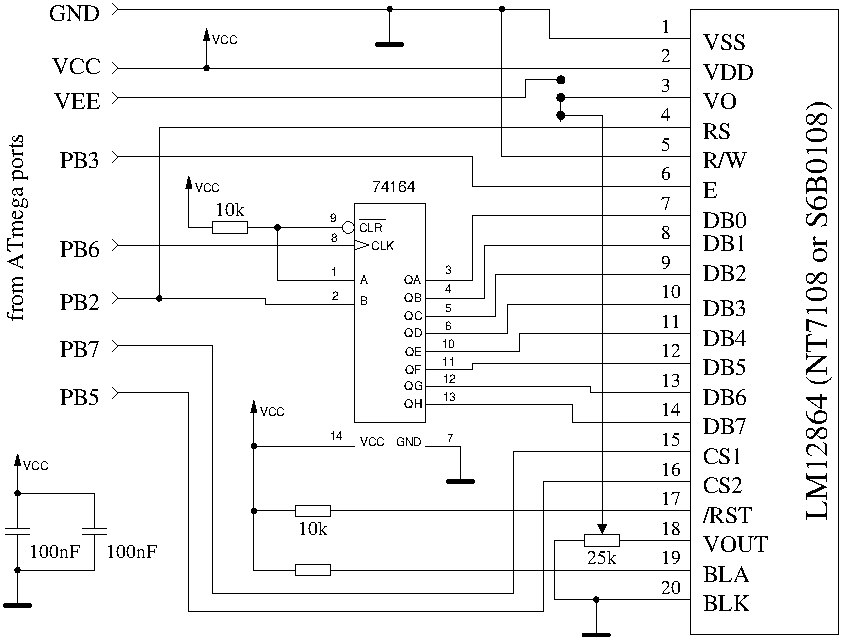
\includegraphics[width=.88\textwidth]{../FIG/ST7108serial164_644.pdf}	% width=8cm
    \caption{mit 74HCT164}
  \end{subfigure}
~
  \begin{subfigure}[b]{.5\textwidth}	% 9cm
    \centering
    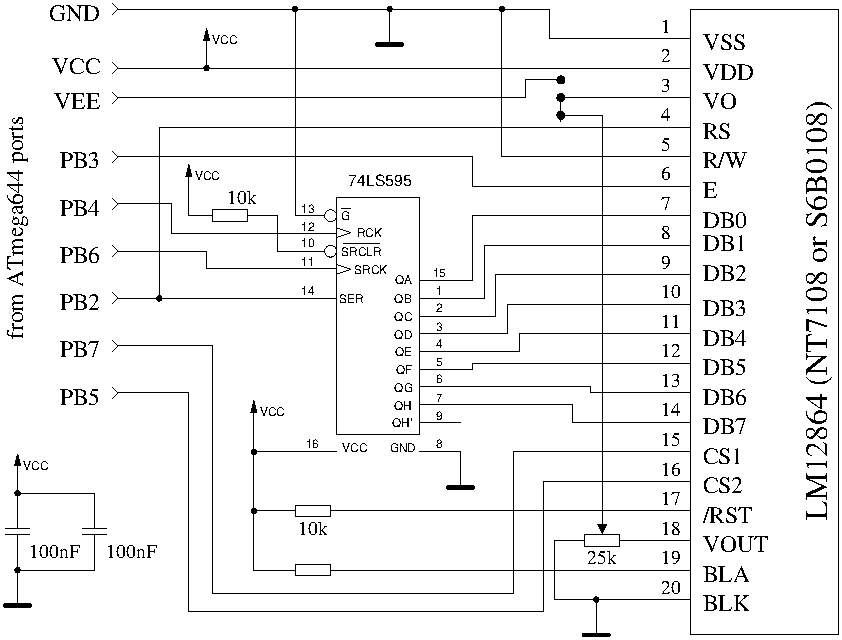
\includegraphics[width=.88\textwidth]{../FIG/ST7108serial595_644.pdf}	% width=8cm
    \caption{mit 74HCT595}
  \end{subfigure}
  \caption{Anschluss des NT7108 Controllers an einen ATmega644/1284}
\label{fig:NT7108lcd_644}
\end{figure}

\begin{figure}[H]
\centering
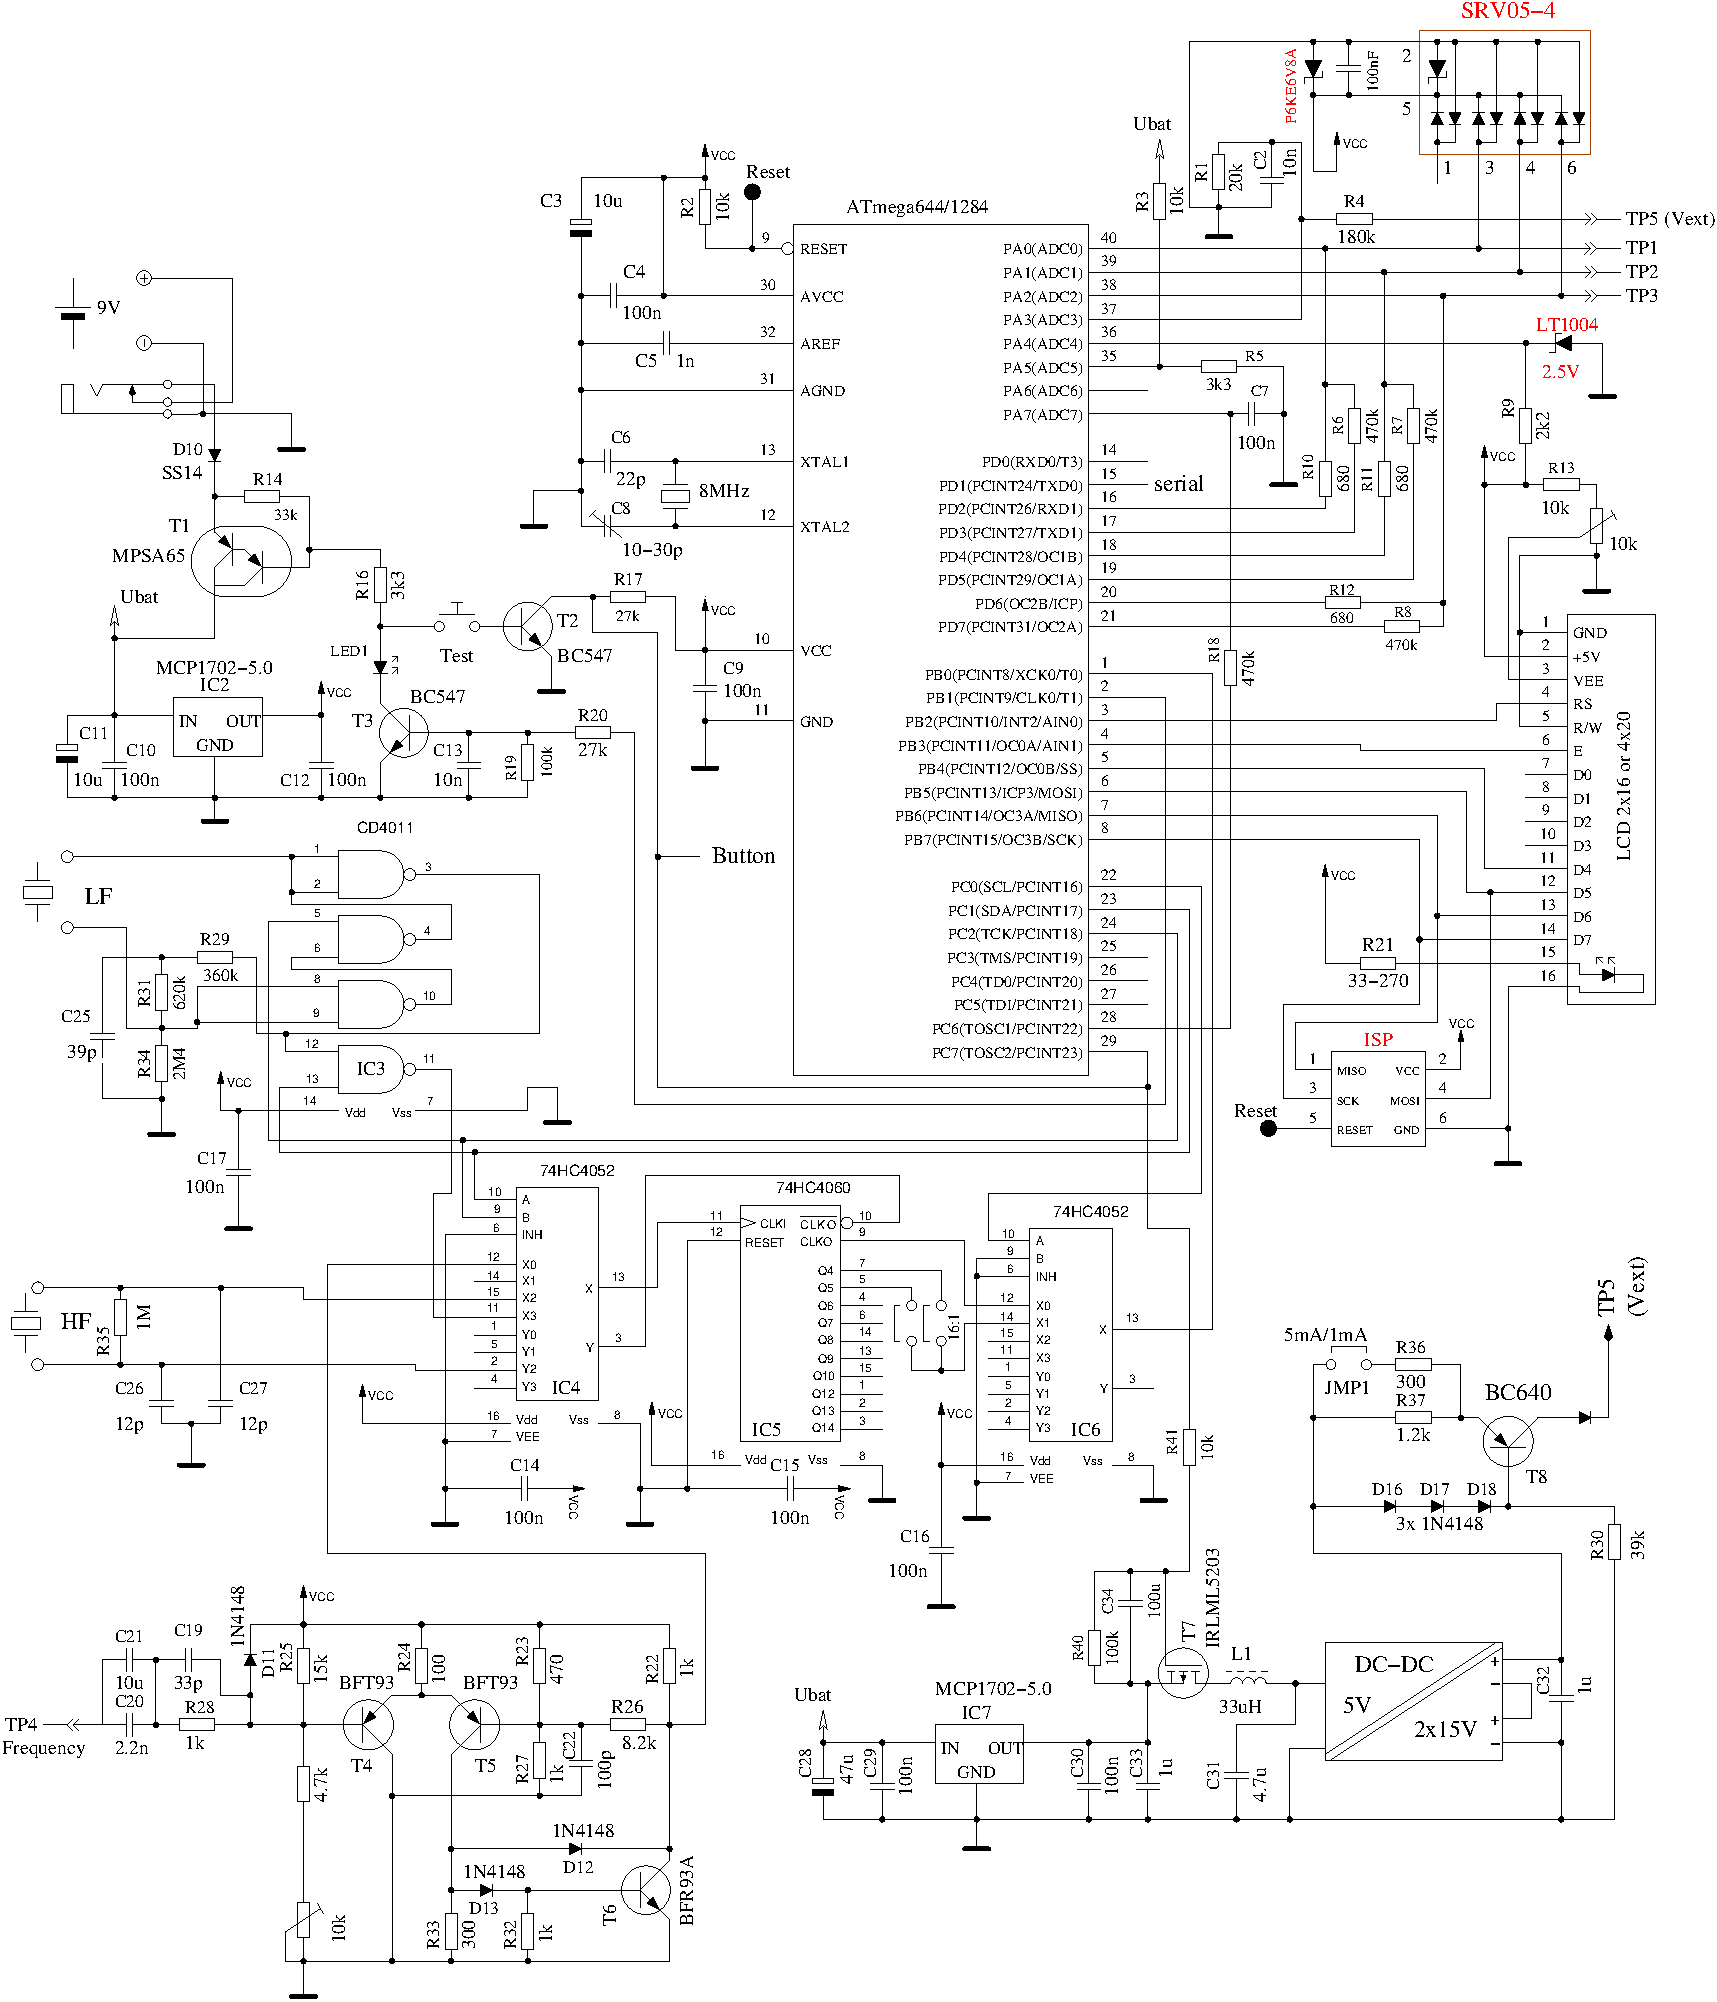
\includegraphics[width=1.\textwidth]{../FIG/t644tester.pdf}	% width=18cm
\caption{Erweiterte Transistortester Schaltung mit ATmega644}
\label{fig:t644tester}
\end{figure}

\section{Aufbau mit ATmega1280 oder Arduino Mega}
Die Grundschaltung des Testers läßt sich auch mit einem Arduino Mega mit ATmega1280 oder
ATmega2560 als Shield aufbauen.
Die notwendigen Verbindungen zeigt die Abbildung~\ref{fig:t1280tester}.
Die Steckverbindungen des Arduino für die Datenverbindungen des Displays sind in güner Farbe eingezeichnet.
Die Bauteile mit roter Bezeichnung sind für die Funktion des Testers nicht erforderlich.
Der ATmega2560 Controller hat zwar viele Anschlußpins, aber nur ein einziger Pin hat die
erforderlichen Verbindungen für beide Methoden der Frequenzmessung.
Der Anschlußpin muß als Takteingang für einen Zähler geschaltet werden können und außerdem muß
der Pin ein Unterbrechungssignal (Interrupt) bei Pegelwechsel erzeugen können.
Dies ist nur für den Pin PE6 (T3/INT6) der Fall. Die anderen Takteingänge der Zähler
PD7 (T0), PD6 (T1), PH7 (T4) und PL2 (T5) können nicht für die Erzeugung des Unterbrechungssignals
bei Pegelwechsel verwendet werden.
Leider ist der PE6 Pin nicht mit den Steckerleisten des Arduino verbunden.
Der PE5 Pin (7) ist mit dem Anschluß 3 der PWM Buchsenleiste des Arduino verbunden und kann
am Atmega2560 mit dem PE6 Pin (8) gebrückt werden.
Der Ausgang der Frequenzerzeugung ist am Pin PB6 (OC1B) verfügbar. Dieser Pin ist mit Anschluß 12
der PWM-Buchsenleiste verbunden.
Auf den ISP-Stecker kann für den Arduino verzichtet werden, da das Programm über
das USB-Interface und den Bootloader geladen werden kann.  Mit dem
Bootloader gibt es lediglich eine kleine Verzögerung des Programmstarts.

\begin{figure}[H]
\centering
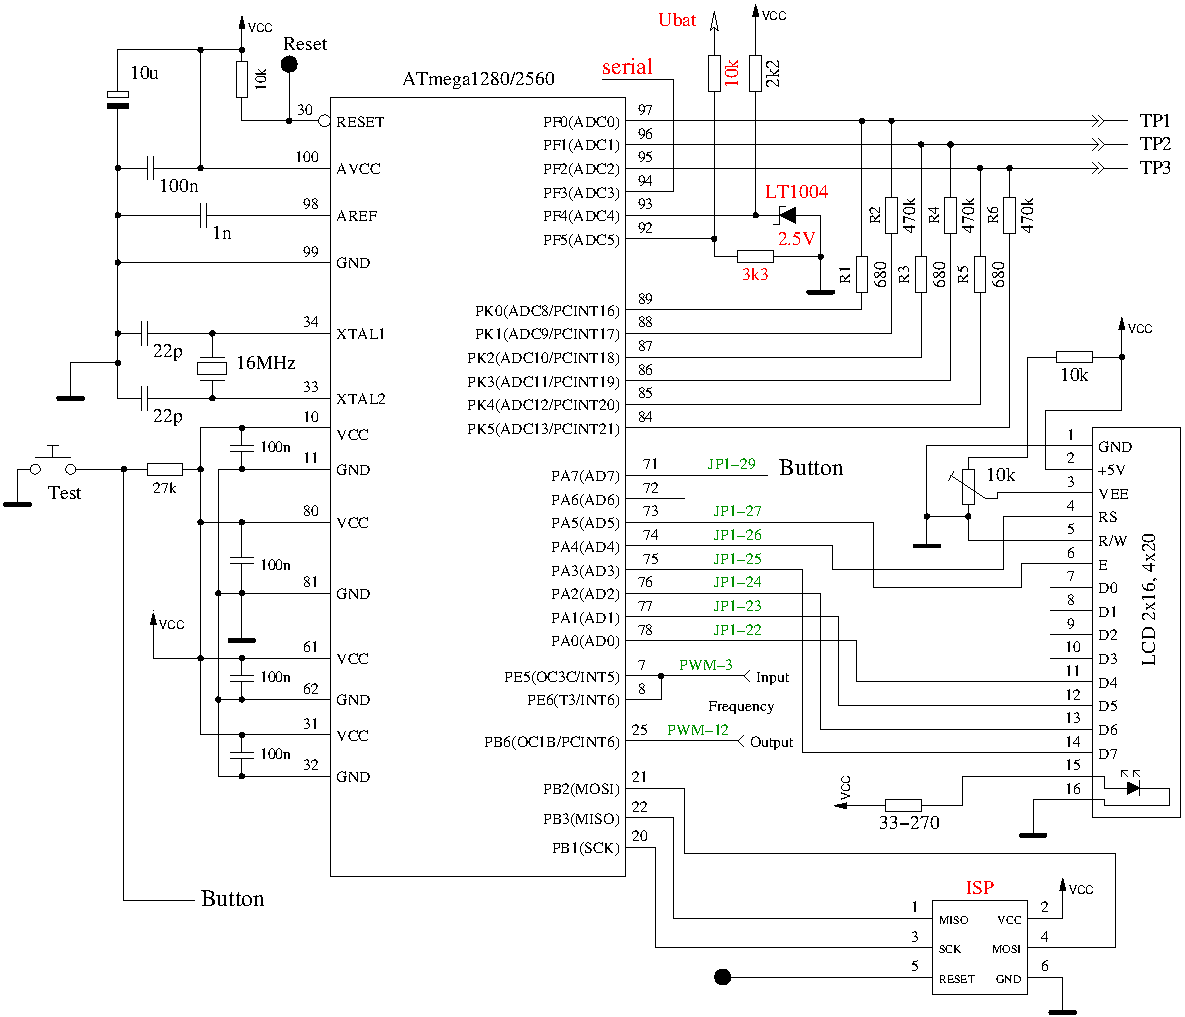
\includegraphics[width=1.\textwidth]{../FIG/t1280tester.pdf}	% width=18cm
\caption{Transistortester Schaltung mit ATmega1280, ATmega2560 oder Arduino Mega}
\label{fig:t1280tester}
\end{figure}

Natürlich können alle unterstützten Displays auch an die ATmega1280 oder ATmega2560 angeschlossen
werden, wie in der Tabelle~\ref{tab:display-1280} angegeben.

\begin{table}[H]
  \begin{center}
    \begin{tabular}{| c || c | c | c | c | c | c |}
    \hline
           & Character     &  ST7565     & ST7920       & NT7108       & SSD1306     & Zusatzfunktion \\
      Port & LCD           &    SPI      & seriell      & seriell      &    I\textsuperscript{2}C      & \\
    \hline
    \hline
    PA0    &  LCD-D4       &   LCD-REST  &  LCD-RESET   & HC595-RCK       &             & \\
    \hline
    PA1    &  LCD-D5       &   LCD-RS    &              & LCD-CS2        &             & Drehgeber-2 \\
    \hline
    PA2    &  LCD-D6       &   LCD-SCLK  &              & HC164-CLK      &             & \\
    \hline
    PA3    &  LCD-D7       &   LCD-SI    &              & LCD-CS1        &             & Drehgeber-1 \\
    \hline
    PA4    &  LCD-RS       &             &   LCD-B0     & LCD-RS         &   LCD-SDA   & \\
           &               &             &              & HC164-SER      &             & \\
    \hline
    PA5    &  LCD-E        &  (LCD-CE)   &   LCD-EN     & LCD-EN         &   LCD-SCL  & \\
    \hline
    PA7    &  Tastensignal &             &              &                &             & \\
    \hline
    \end{tabular}
  \end{center}
  \caption{Pinbelegungen für verschiede Displays an ATmega1280/2560}
\label{tab:display-1280}
\end{table}

\section{Chinesische Nachbauten mit Textdisplay}
Der Tester wird in China nach meinem Kenntnisstand in zwei Versionen mit Textdisplay nachgebaut.
Die erste Variante ist der Nachbau des ersten Entwurfs von Markus F. ohne ISP-Schnittstelle.
Der bestückte ATmega8 ist bei dieser Version gesockelt, kann also auch durch einen ATmega168/328 ausgetauscht werden.
Für diese Version gelten alle Hinweise des Unterkapitels~\ref{sec:change_markus}.
Zusätzliche \(100nF\) keramische Kondensatoren sollten in der Nähe des ATmega an die VCC-GND und
AVCC-GND Anschlüsse zur besseren Spannungsstabilisierung angebracht werden.
Da auf der Platine ein ISP-Stecker fehlt, muß entweder ein ISP-Anschluß nachgerüstet werden oder
der Prozessor für die Programmierung ausgebaut werden.
Dabei muss beachtet werden, dass bei der Nachrüstung eines Quarzes der ISP-Programmer selbst
einen externen Takt zuführen muss, oder der Programmiersockel mit einem Quarz ausgerüstet sein muß.\\
Die zweite Variante ist weitgehend in SMD-Technik aufgebaut. Auch der ATmega168 oder ATmega328 
ist in einem 32TQFP Gehäuse fest verbaut.
Dafür ist ein 10-poliger ISP-Stecker für die Programmierung auf der Platine vorgesehen.
Ich habe die Version \inquotes{2.1 2012/11/06} analysiert. Ein Fehler ist die Bestückung des Bauteils \inquotes{D1},
welches eigentlich die \(2,5V\) Präzisionsreferenz sein soll. Bestückt ist aber eine Zenerdiode.
Dieses Bauteil sollte entfernt werden. Hier kann eine Präzisionsreferenz wie LM4040AIZ2.5 oder
LT1004CZ-2.5 angeschlossen werden. Eine fehlende Präzisionsreferenz wird von der Software erkannt,
so dass sie nicht unbedingt erforderlich ist.
Bei meinem Exemplar war die Software Version 1.02k installiert. Der 10-polige ISP-Stecker war nicht
bestückt und ich musste zusätzlich eine Brücke von Pin 10 nach Pin 6 nachlöten. Mein Programmer hat eine 
GND-Verbindung an Pin 10 erwartet, der Tester hatte aber nur bei Pin 4 und Pin 6 eine GND-Verbindung.
Die Beschriftung des ATmega168 war abgeschliffen und es gab keine Dokumentation zum Gerät.
Die Sicherheits-Bits des ATmega waren gesetzt, sodass sich das Programm nicht auslesen ließ.
Ich konnte aber problemlos die Software Version 1.05k installieren.
Die gleiche Softwareversion 1.05k hat bei einem anderen Nutzer mit der China-Version \inquotes{2.2 2012/11/26} Probleme
gemacht. Die Software 1.05k lief hier erst, als ein weiterer \(100nF\) SMD Kondensator zwischen die Pins 18-AVCC
und 21-GND ergänzt wurde. Die Software 1.05k benutzt bei Wartezeiten den Schlafzustand des ATmega.
Deswegen wechselt der Strombedarf häufiger und der Spannungsregler wird mehr beansprucht.
Aufgefallen ist mir weiter, dass die VCC-Spannung mit einem \(100nF\) keramischen Kondensator und mit
einem \(220\mu F\) elektrolytischen Kondensator in der Nähe des 78L05-Spannungsreglers abgeblockt ist.
Die \(9V\) Spannungszufuhr ist mit den gleichen Kondensatoren abgeblockt, allerdings am Emitter des PNP-Transistor
(parallel zur Batterie), nicht direkt am Reglereingang.
Die Leiterbahnen vom ATmega zu den Testports sind teilweise sehr dünn, sodass ich einen Widerstand
von etwa \(100m\Omega\) pro Signalweg messen konnte. Dies ist wohl mit der Grund dafür, dass zwei
mit \(0\Omega\) verbundene Pinne einen Widerstandswert von \(0,3\Omega\) messen.
Bei der ESR-Messung kann dies normalerweise durch den Nullabgleich kompensiert werden.
Bei der Messung von Widerständen unter \(10\Omega\) werden die im Selbsttest ermittelten Offsets 
ab der Softwareversion 1.07k berücksichtigt.

\section{Chinesische Nachbauten mit graphischem Display}
Neuere Nachbauten verwenden ein 128x64 Pixel graphisches Display wie zum Beispiel eine Version von Fish8840.
Bei dieser Version wird eine veränderte Schaltung für das Einschalten benutzt. Die Abbildung~\ref{fig:Fish8840}
zeigt einen Ausschnitt der Schaltung.

\begin{figure}[H]
\centering
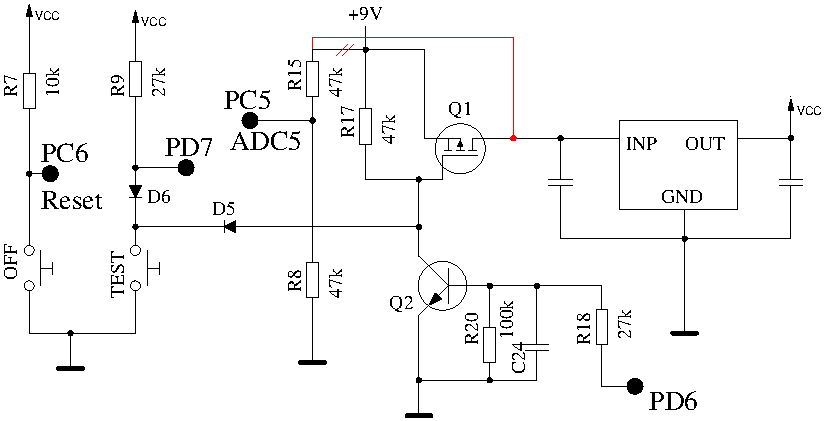
\includegraphics[width=.7\textwidth]{../FIG/Fish8840.pdf}	% width=12cm
\caption{Ausschnitt aus der Schaltung von Fish8840}
\label{fig:Fish8840}
\end{figure}

Wie an den Widerständen R8 und R15 zu erkennen ist, 
wird mit 2:1 ein anderes Teilerverhältnis für die Batteriespannung wie im Original verwendet.
Außerdem ist R15 direkt an die Batterie angeschlossen, was zu einem geringen Stromverbrauch im
ausgeschalteten Zustand führt. Hier sollte R15 besser an das Drain von Q1 beziehungsweise an den
Eingang des Spannungsreglers angeschlossen werden um den unnötigen Batterieverbrauch zu vermeiden.
Eine entsprechende Änderung auf der Platine zeigt die Abbildung~\ref{fig:Fish8840patch}.
Eine Leiterbahn ist zwischen R17 und D5 getrennt und mit einem Stück Kupferlackdraht eine
neue Verbindung zwischen Q1 und R15 gelötet.

\begin{figure}[H]
\centering
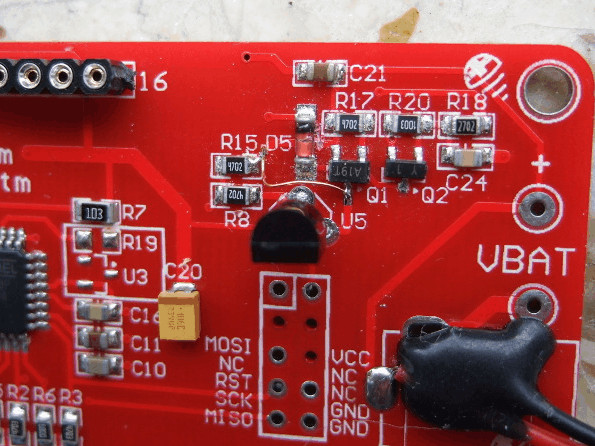
\includegraphics[width=.7\textwidth]{../PNG/Fish8840patch.jpg}	% width=12cm
\caption{Foto der geänderten Fish8840 Platine}
\label{fig:Fish8840patch}
\end{figure}

Das Verhältnis des Spannungsteilers muss bei der Konfiguration in der Makefile auf jeden Fall angegeben
werden bevor eine Software aufgespielt wird (z.B. mit BAT\_NUMERATOR=66).

Das Display Module des Fish8840 Testers besitzt einen \(3.3V\) Spannungsregler, der die Betriebsspannung
des Display-Controllers anpassen soll.
Da es über die Datenleitungen des Display-Moduls zu einer Erhöhung der \(3.3V\) Betriebsspannung wegen
der \(5V\) Signale vom ATmega kommt,
wird eine Adapterschaltung nach Abbildung~\ref{fig:Fish8840Adapt} empfohlen. Hier sind in die vier
Datenleitungen vier serielle Widerstände mit jeweils \(2.7k\Omega\) auf einer kleinen Lochrasterplatine
zwischengeschaltet.
Längere Gewindebolzen müssen nun verwendet werden, um das Display mit der Adapterplatine auf dem
Fish8840 Tester zu befestigen.

\begin{figure}[H]
  \begin{subfigure}[b]{.5\textwidth}	% width=9cm
    \centering
    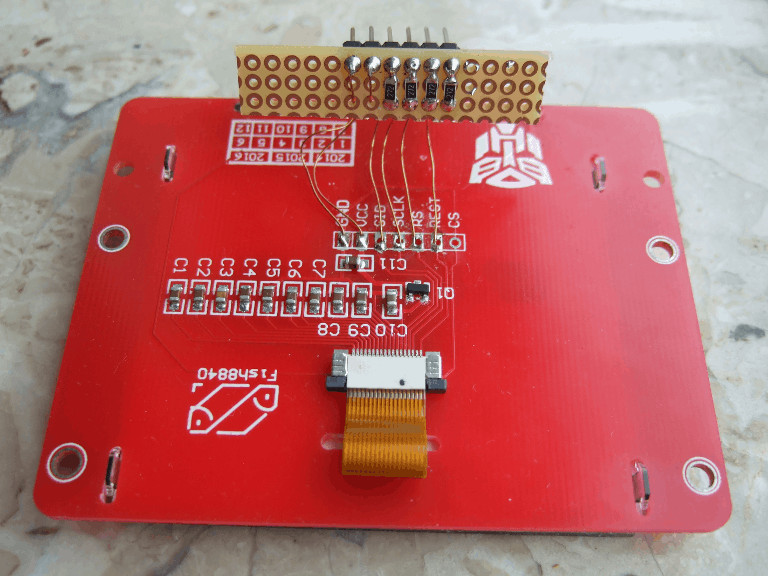
\includegraphics[width=1.\textwidth]{../PNG/Fish8840Adapt1.jpg}	% width=9cm
    \caption{Display mit Adapter}
  \end{subfigure}
~
  \begin{subfigure}[b]{.5\textwidth}	% width=9cm
    \centering
    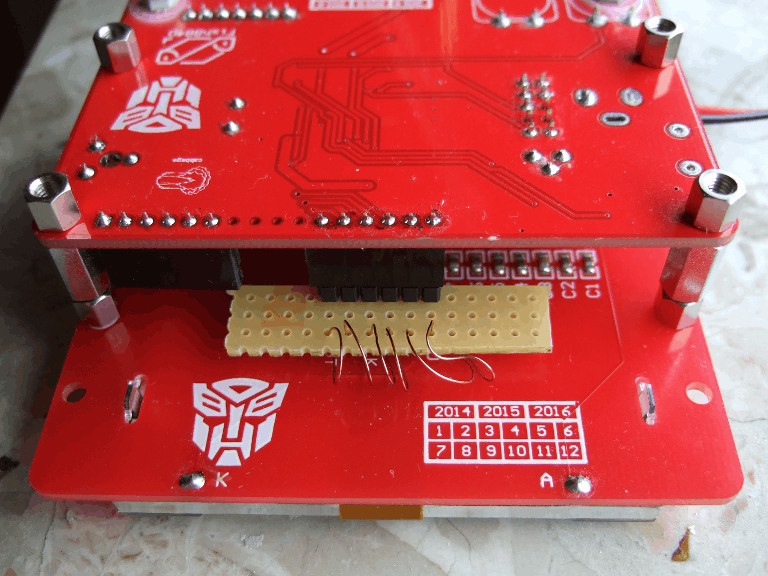
\includegraphics[width=1.\textwidth]{../PNG/Fish8840Adapt2.jpg}	% width=9cm
    \caption{Fertig montierter Tester}
  \end{subfigure}
  \caption{Adapter für einen korrekten Display Anschluß}
\label{fig:Fish8840Adapt}
\end{figure}

Anstelle dieser Umrüstung kann mit der Makefile Option LCD\_SPI\_OPEN\_COL auch eine spezielle Ausgangsschaltung
der 4~SPI Signale des ATmega benutzt werden.
Dabei werden die Ausgänge nicht auf VCC Pegel geschaltet,
sondern nur die internen \inquotes{Pull-Up} Widerstände während der Ausgabe für den high Pegel freigeschaltet.
Wenn die Option PULLUP\_DISABLE gesetzt ist, ist ein externer Pull-Up Widerstand für das
Reset Signal (PD0) erforderlich.
Weil die Datensignale nie direkt auf VCC geschaltet werden, kann die \(3.3V\) Versorgung des LCD-Controllers
auch nicht überhöht werden.
Die mir vorliegende Platine des Fish8840 Testers hat alle Signale für den Anschluß eines
Textdisplays an die LCD-Steckerleiste geführt. 
Deshalb kann die Platine auch mit einem Textdisplay umgerüstet werden, wenn die Buchsenleiste
ergänzt wird und das Potentiometer für die Kontrasteinstellung nachgerüstet wird.
Der Versorgungspin 15 für die Hindergrundbeleuchtung ist allerdings direkt mit VCC verbunden.
Bei einer Installation eines Textdisplays sollte darauf geachtet werden, daß auf dem Displaymodul
ein serieller Widerstand zur LED vorhanden ist.
Selbstverständlich muß die Software für eine andere Displayversion angepasst werden.
Auch die Erweiterungsmöglichkeiten des Testers sind bei der Fish8840 Platine möglich.\\

Für die Funktionsfähigkeit kann natürlich keine Gewähr gegeben werden.
Leider kann der Originalzustand der chinesischen Software-Variante auch nicht gesichert werden,
da die Sicherheits-Bits des ATmega328 gesetzt sind.
Es gibt also keinen Weg zurück zur Originalversion der Software.\\ 

Eine weitere Version mit graphischem Display ist die WEI\_M8 Platine, die in Abbildung~\ref{fig:WeiM8}.
Dieser Nachbau benutzt als Stromquelle einen LiIon Akkumulator im AA (Mignon) Format, der über
eine Micro-USB Schnittstelle geladen werden kann. Ein Betrieb ohne Akku ist über die USB-Schnittstelle
ebenfalls möglich.

\begin{figure}[H]
\centering
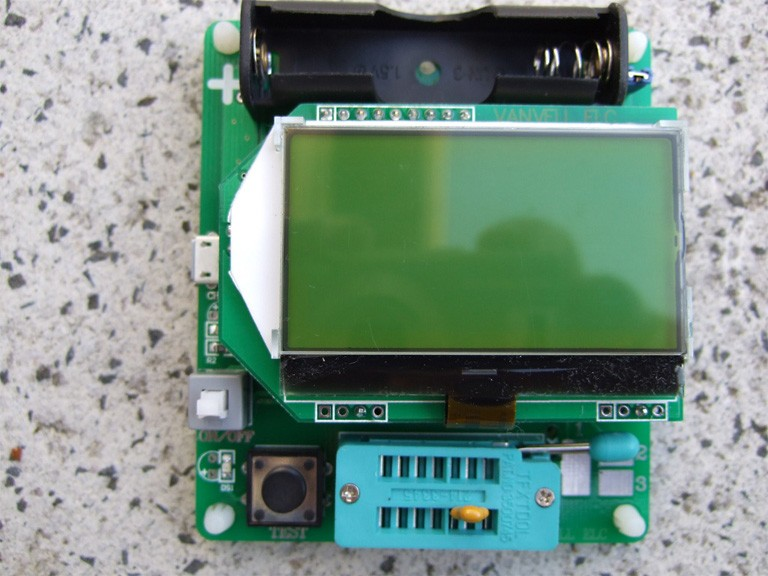
\includegraphics[width=.7\textwidth]{../PNG/WEI_M8.JPG}	% width=12cm
\caption{Foto des chinesischen WEI\_M8 Testers}
\label{fig:WeiM8}
\end{figure}

Erfreulich ist, dass für die Signalleitungen des Displays serielle Widerstände
auf der Adapterplatine vorgesehen sind, wie in der linken Abbildung von~\ref{fig:WeiM8int}
zu sehen ist. Damit ist eine Überhöhung der \(3.3V\) Versorgung für den Displaycontroller
wegen der \(5V\) Signalpegel vom ATmega nicht zu befürchten.

\begin{figure}[H]
  \begin{subfigure}[b]{.5\textwidth}	% 9cm
    \centering
    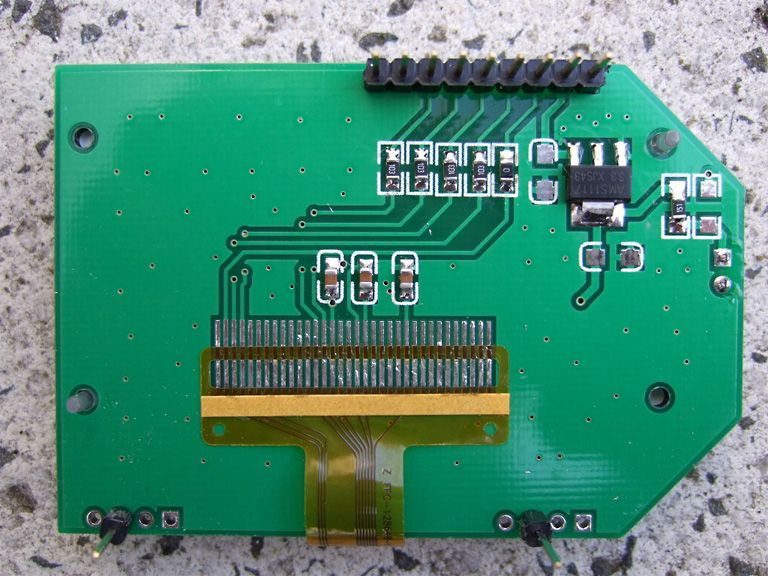
\includegraphics[width=1.\textwidth]{../PNG/WEI_M8_D.JPG}	% width=9cm
    \caption{Adapterplatine für das Display}
  \end{subfigure}
~
  \begin{subfigure}[b]{.5\textwidth}	% 9cm
    \centering
    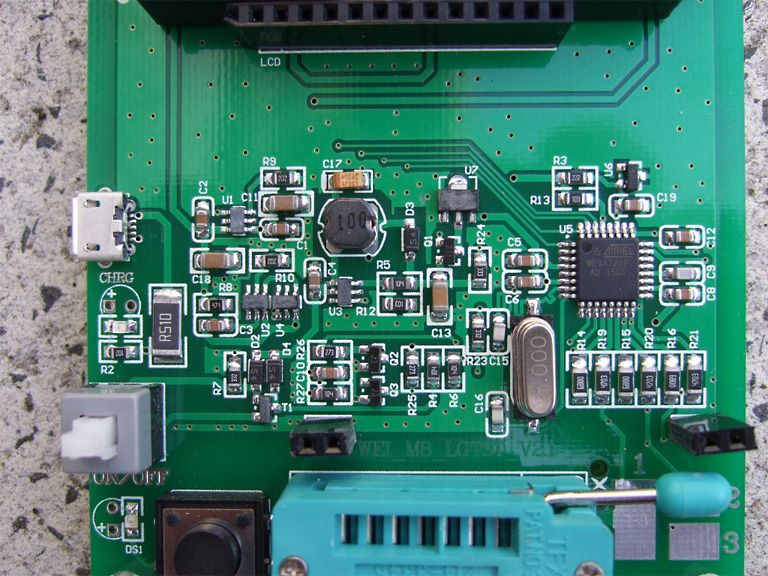
\includegraphics[width=1.\textwidth]{../PNG/WEI_M8_L.JPG}	% width=9cm
    \caption{Grundplatine}
  \end{subfigure}
  \caption{Innenleben des WEI\_M8 Testers}
\label{fig:WeiM8int}
\end{figure}


Bei der Aufrüstung auf die 1.12k Version
der Software ergaben sich einige Schwierigkeiten. Wenn die extended Fuse wie empfohlen auf
0x04 (oder 0xfc) gesetzt wird, kam es bei bestimmten Messungen zu \inquotes{Brown Out} Resets des
Prozessors. Diese Resets werden durch kurzzeitige Spannungseinbrüche der VCC Versorgung
verursacht. Die Platine wurde deshalb mit einem \(4.7\mu F\) kermamischen Kondensator
am Eingang des Spannungsreglers und mit einem \(10\mu F\) keramischen Kondensator am
Reglerausgang (VCC) zusätzlich abgeblockt. Sowohl vor der Nachrüstung als auch danach
wurde bei bipolaren Transistoren ein Kollektor-Reststrom (ICEO oder ICEs) gemessen.
Erst der Austausch des LDO-Spannungsreglers (unbekannter Typ) durch einen MCP1702-5002
brachte hier Abhilfe. Die Abbildung~\ref{fig:WeiM8mod} zeigt die umgerüstete Platine
mit den schräg montierten nachgerüsteten Kondensatoren und dem MCP1702 Regler.
Wer die Kondensatoren nicht nachrüsten möchte, sollte die extended Fuse auf 0x07 (0xff)
setzen, damit ein Betrieb möglich ist. Damit bleiben die Spannungseinbrüche unentdeckt.

\begin{figure}[H]
\centering
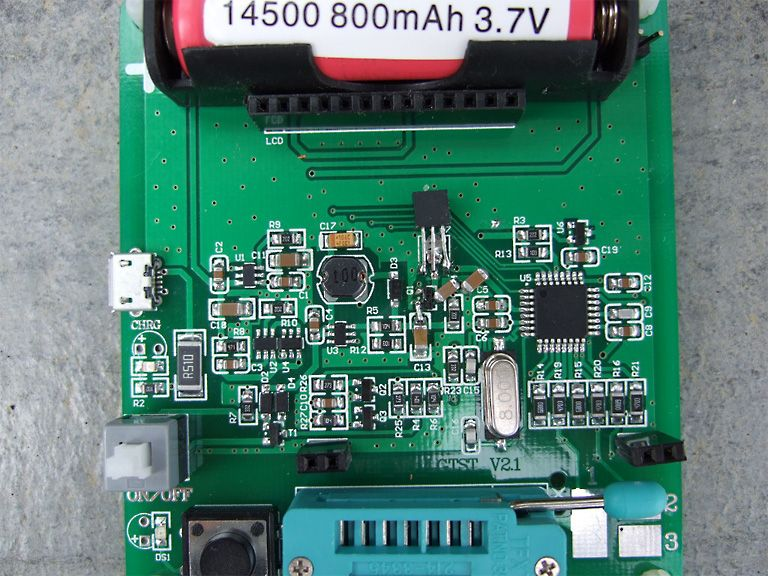
\includegraphics[width=.7\textwidth]{../PNG/WEI_M8_modified.JPG}	% 12cm
\caption{Foto des umgerüsteten WEI\_M8 Testers}
\label{fig:WeiM8mod}
\end{figure}

Eine weitere Version mit graphischem Display ist der LCD-T4 Tester mit einer gelben Platine.
Für das Aufspielen neuer Software habe ich das Display abgenommen.
Auf dem rechten Foto der Abbildung~\ref{fig:T4_front} ist der Stecker für die ISP-Verbindung rechts oben
 neben den entsprechen Bohrungen der Platine in der richtigen Ausrichtung aufgelegt.
Für die Programmierung habe habe ich den Stecker nicht eingelötet, sondern nur eingesteckt und durch
seitlichen Druck mit einem Finger für die Dauer der Programmierung fixiert.
Dadurch kann der Stecker nach der Programmierung wieder leicht entfernt werden und das Display
an die ursprüngliche Stelle montiert werden.
Die Software 1.12k konnte übrigens problemlos aufgespielt werden.
Auch das Aktivieren der \inquotes{Brown-Out} Erkennung des Prozessors mit der extended fuse
brachte keine Überraschungen.

\begin{figure}[H]
  \begin{subfigure}[b]{.5\textwidth}	% 9cm
    \centering
    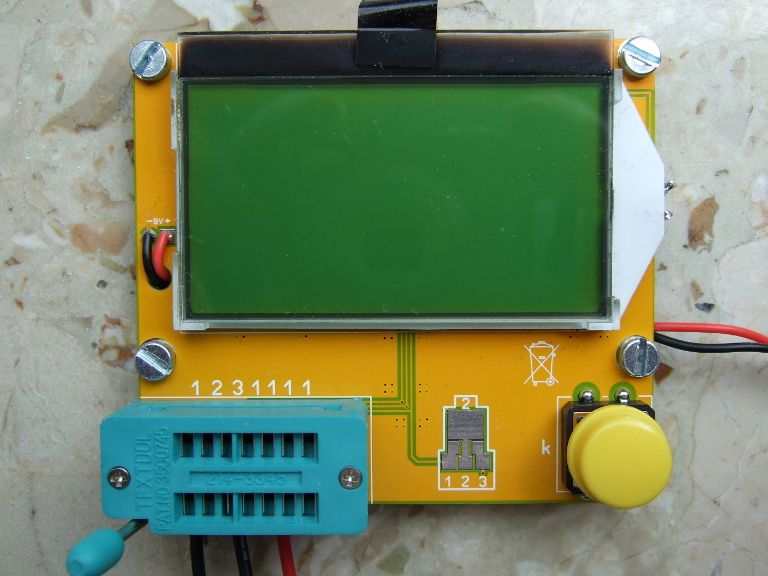
\includegraphics[width=1.\textwidth]{../PNG/T4_front.JPG}	% width=9cm
    \caption{vollständig}
  \end{subfigure}
~
  \begin{subfigure}[b]{.5\textwidth}	% 9cm
    \centering
    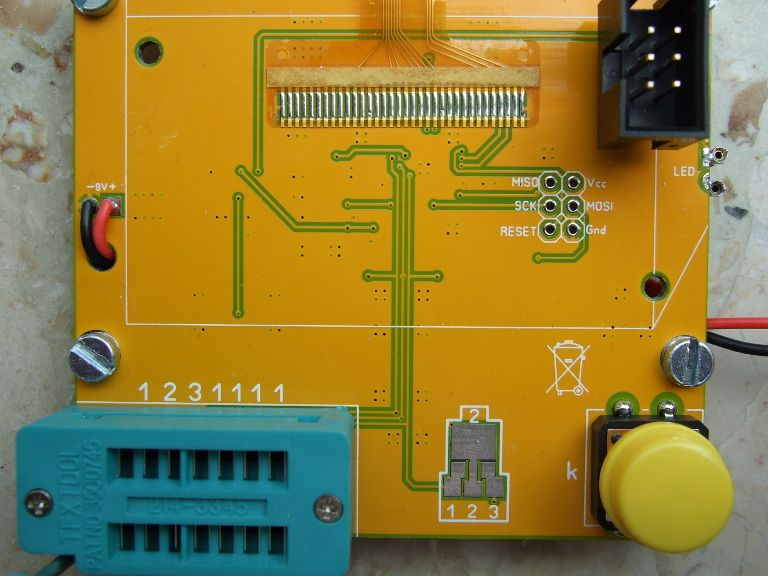
\includegraphics[width=1.\textwidth]{../PNG/T4_front_noLCD.JPG}	% width=9cm
    \caption{mit abgenommenem Display}
  \end{subfigure}
  \caption{Frontansicht des T4 Testers}
\label{fig:T4_front}
\end{figure}

Auf den Fotos der Rückseite in Abbildung~\ref{fig:T4_back} sieht man die nachgerüsteten
\(5mm\) Gewindebolzen sowie die nachträglich angelöteten Kabel mit Messclips.
Da aber für die Datensignale des graphischen LCD-Controllers auch hier
keine Signalanpassung (\(5V~-\textgreater ~3.3V\)) erfolgt, ist das Setzen der Option LCD\_SPI\_OPEN\_COL ratsam.
Da die Nachrüstung eines \inquotes{pull-up} Widerstandes für das SPI-Reset Signal hier
aber schwierig durchzuführen ist, bleibt nur das Entfernen der Option
DISABLE\_PULLUP übrig. 
Für nachträgliche Erweiterungen ist diese Platine weniger geeignet, auch ein Austausch des
Displays ist hier nur schwer möglich.

\begin{figure}[H]
  \begin{subfigure}[b]{.5\textwidth}	% 9cm
    \centering
    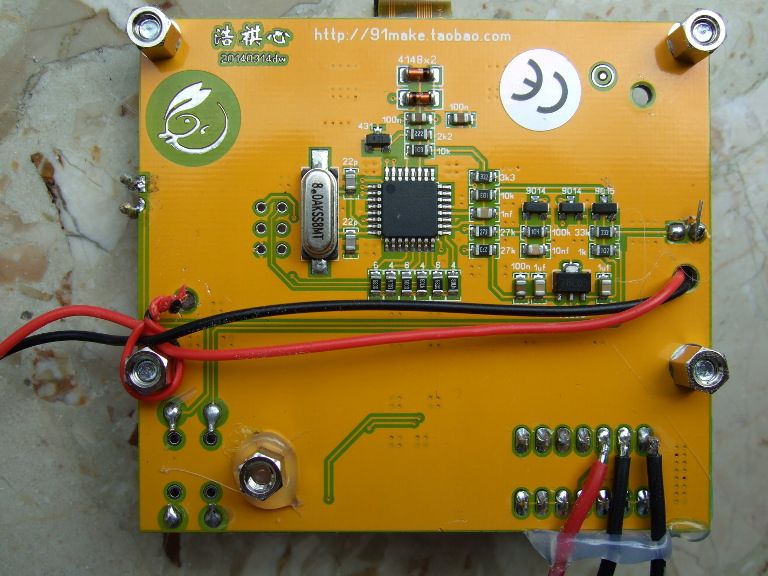
\includegraphics[width=1.\textwidth]{../PNG/T4_back.JPG}	% width=9cm
    \caption{Bestückungsseite}
  \end{subfigure}
~
  \begin{subfigure}[b]{.5\textwidth}	% 9cm
    \centering
    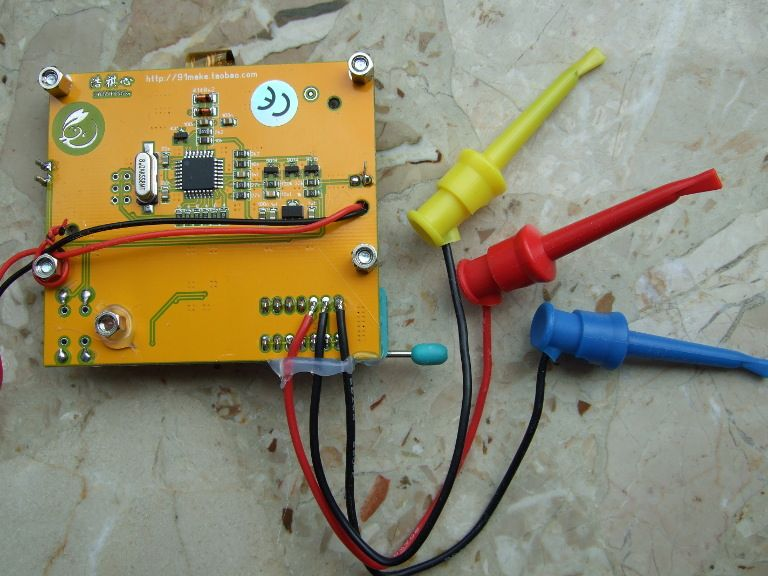
\includegraphics[width=1.\textwidth]{../PNG/T4_back_clips.JPG}	% width=9cm
    \caption{mit Messkabeln}
  \end{subfigure}
  \caption{Rückansicht des T4 Testers}
\label{fig:T4_back}
\end{figure}

Noch eine chinesische Version mit graphischem Display wird mit der Bezeichnung \inquotes{GM328} angeboten.
Bei dieser Version ist das graphische Display an eine 16-pol Buchsenleiste mit einer Tochterplatine
angeschlossen.
Dabei ist auch der Port PD5 über die Buchsenleiste Pin 6 an das CE (Chip Enable) Signal
des graphischen Controllers angeschlossen. Das CE Signal ist aber auf der Tochterplatine auch mit der
\(0V\) Power (GND) verbunden.
Das führt zu einem Kurzschluß, wenn der ATmega den PD5 Ausgang auf \(5V\) schalten möchte.
Neuere Versionen der Software schalten aber auch das CE Signal, auch wenn das Signal für den Betrieb nicht
benötigt wird.
Deswegen sollte bei dem \inquotes{GM328} Tester die Verbindung der Tochterplatine zum Pin 6 
der Anschlußleiste unterbrochen werden.

\section{Chinesische Bausätze mit Grafikdisplay}

Bisher sind zwei Bausätze mit grafischen Display und Drehimpulsgeber bekannt.
Der zuerst erschienene Bausatz verwendet ein Display mit ST7565 oder kompatiblen Controller (128x64 Pixel).
Außer dem Drehimpulsgeber ist  auch ein Eingang für die Frequenzmessung vorgesehen.
Für die Testports steht ein 14-poliger Textool Sockel, 3 Lötaugen für Kabel sowie ein Testpad
für SMD Bauteile zur Verfügung. 
Die Fotos~\ref{fig:Kit_mono} zeigen den zusammengebauten Bausatz.
Einer der beiden \(22 pF\) Kondensatoren 
wurde hier durch einen Trimmer auf der Lötseite ersetzt. Mit dem Trimmer läßt sich die Frequenz des Quarzes für genauere
Frequenzmessung bzw. Frequenzerzeugung abgleichen.

\begin{figure}[H]
  \begin{subfigure}[b]{.5\textwidth}	% 9cm
    \centering
    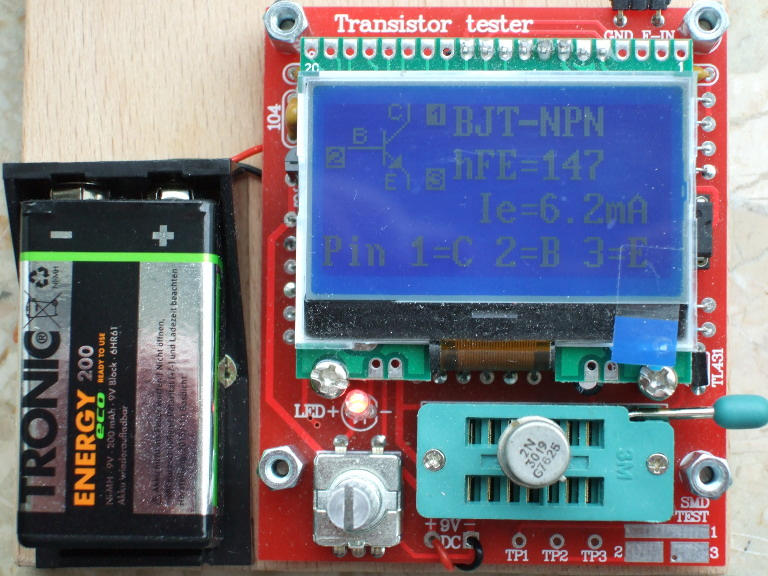
\includegraphics[width=1.\textwidth]{../PNG/Kit_ST7565a.jpg}	% width=9cm
    \caption{zusammengebaut}
  \end{subfigure}
~
  \begin{subfigure}[b]{.5\textwidth}	% 9cm
    \centering
    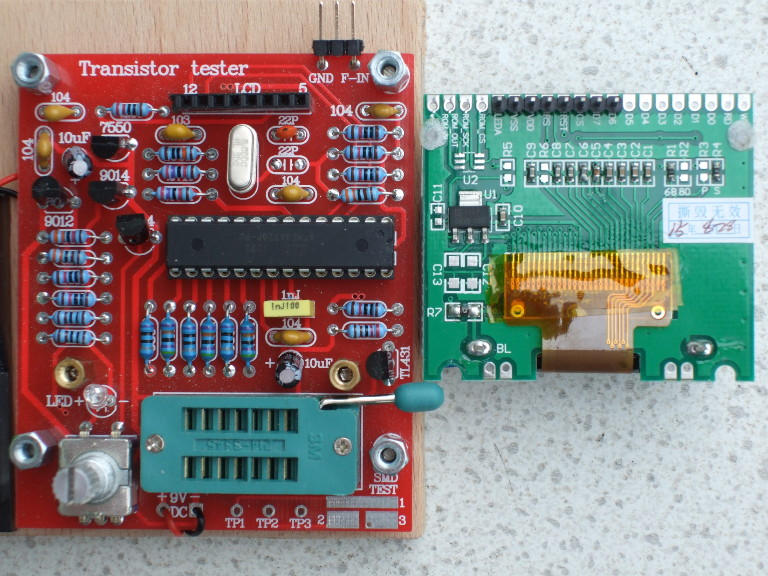
\includegraphics[width=1.\textwidth]{../PNG/Kit_ST7565b.jpg}	% width=9cm
    \caption{mit abgenommenem Display}
  \end{subfigure}
  \caption{Bestückter Bausatz mit 128x64 Pixel Display}
\label{fig:Kit_mono}
\end{figure}

Der später erschienene Bausatz verwendet ein Farbdisplay mit ST7735 Controller (128x160 Pixel) 
und hat zusätzlich zum Fequenzeingang noch einen Eingang für Spannungsmessung und einen Frequenzausgang.
Der Frequenzausgang ist aber nicht gepuffert, sondern ist lediglich zum Anschluß TP2 parallel 
angeschlossen. Bei der Spannungsmessung handelt es sich nur um die Messung einer positiven Gleichspannung bis 50V,
ein DC-DC Wandler für die Zenerspannungsmessung wurde nicht vorgesehen.
Die Fotos~\ref{fig:Kit_color} zeigen den zusammengebauten Bausatz.
Auch hier wurde einer der beiden \(22 pF\) Kondensatoren 
wurde hier durch einen Trimmer (grün) ersetzt. 

\begin{figure}[H]
  \begin{subfigure}[b]{.5\textwidth}	% 9cm
    \centering
    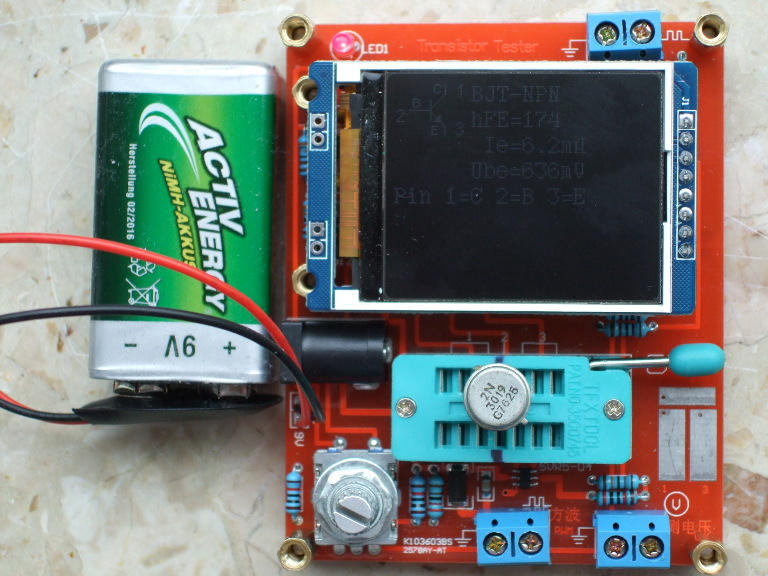
\includegraphics[width=1.\textwidth]{../PNG/Kit_Color_a.jpg}	% width=9cm
    \caption{zusammengebaut}
  \end{subfigure}
~
  \begin{subfigure}[b]{.5\textwidth}	% 9cm
    \centering
    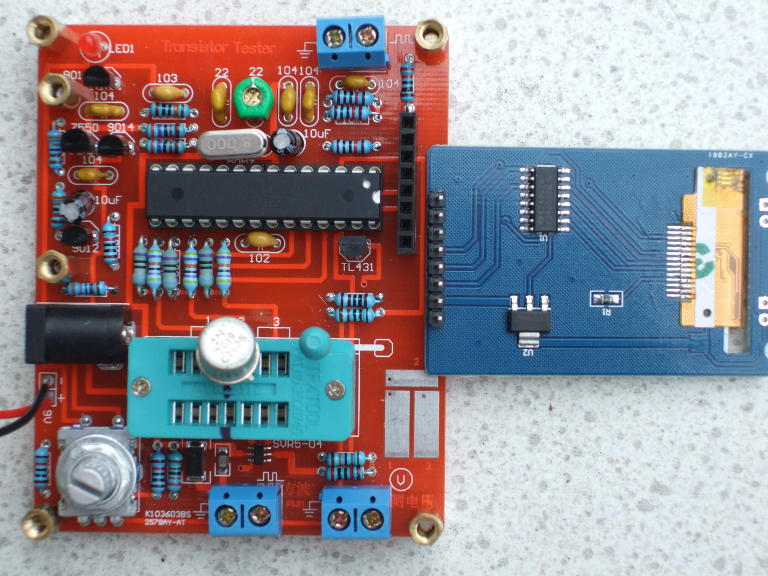
\includegraphics[width=1.\textwidth]{../PNG/Kit_Color_b.jpg}	% width=9cm
    \caption{mit abgenommenem Display}
  \end{subfigure}
  \caption{Bestückter Bausatz mit 160x128 Pixel Farbdisplay}
\label{fig:Kit_color}
\end{figure}

Beide Bausätze verwenden einen gesockelte DIP Version des ATmega328P und haben keinen 
ISP Stecker für das Aufspielen neuer Softwareversionen.
Die erste Version verwendet
ausschließlich bedrahtete Bauteile für die Hauptplatine. Die Meßwiderstände \(680\Omega\) und \(470k\Omega\)
waren bei meinem Bausatz mit einer 0.1\% Toleranz geliefert worden.
Selbst ein \(220 nF\) Kondensator für die Kalibration wurde bei diesem Bausatz mitgeliefert.
Der Bausatz mit dem Farbdisplay hat zusätzlich zum Anschluß für die 9V Batterie noch eine Buchse
für einen Netzteilanschluß. Die wenigen SMD-Bauteile waren schon auf der Platine bestückt,
so daß auch bei diesem Bausatz nur einfache Lötarbeiten durchzuführen sind.
Ein kleiner Nachteil der Version mit dem Farbdisplay ist die Geschwindigkeit der Ausgabe.
Speziell bei der Menübedienung fällt die deutlich langsamere Ausgabe negativ auf.
Andererseits hat das Farbdisplay eine deutlich höhere Pixelzahl und kann damit mehr Text darstellen. 
Beide Bausätze verwenden einen 3.3V Spannungsregler für die Versorgung der Display Controller auf
den vollständig bestückten Display-Platinen. Lediglich die Stiftleiste muß bei
der Displayplatine eingelötet werden.
Die Farbversion verwendet einen CD4050 Puffer für die Anpassung der Signalpegel.
Auf der Display-Platine der ST7565 Variante ist keine Anpassung der Signalpegel erkennbar.
Wahrscheinlich toleriert die gewählte Controller-Variante die 5V Signalpegel des ATmega328.
Es ist jedenfalls keine Schutzdiode gegen die 3.3V Versorgung bei diesem Controller feststellbar.

\section{Und noch ein Clone von Hiland M644}
\label{sec:hiland}
Dieses Nachbau basiert auf dem Schaltplan von Nick L. aus der Ukraine siehe Abbildung~\ref{fig:t644tester}
auf der Seite~\pageref{fig:t644tester}.\\
Bedient wird der Tester mit einem Knopf, der sowohl \textbf {Taster} als auch \textbf {Drehgeber} ist.

Er bietet folgende Zusätze:
\vspace{-0.5\baselineskip}
\begin{itemize} \setlength{\itemsep}{-0.5\baselineskip}
 \item die Frequenzmessung
 \item den f-Generator
 \item 10-bit PWM
 \item Impulsdrehgeber
 \item die Quarz-Messung
 \item Spannung und Zehnerdioden Bestimmung (bis fast 50V).
\end{itemize}
\vspace{-0.5\baselineskip}
Die Platine ist mit einem 8MHz Quarz bestückt. Besser wäre wohl ein 16MHz Quarz,
wobei die Nachrüstung eines Trimmers (genauere Frequenz) schwierig ist.
Die Kontakte für die ISP-Schnittstelle sind auf eine 6-pol Lochreihe unterhalb dem
steckbaren Display-Modul herausgeführt die folgend belegt ist:\\
\textbf {von links nach rechts}: 1~-Reset; 2~-SCK; 3~-MISO; 4~-MOSI; 5~-+5V; 6~-GND.\\
Um den Tester, aktualisieren zu können, benötigt man ein angepasstes Kabel, der man relativ einfach
selbst erstellen kann.
Bei der Auslieferung ist der Nullkraft-Testsockel über Buchsenleisten mit der Platine verbunden.

Bei dem unten abgebildeten Tester wurde der Sockel direkt angelötet und die hiermit gesparte Buchsenleiste
auf ein vorhandenes Flachbandkabel mit Pfostenstecker angelötet und mit Schrumpfschlauch fixiert.
\begin{figure}[H]
 \centering
 \begin{overpic}[width=.64\textwidth]{../FIG/Kabel_Hiland.pdf}
  \color{black}
  \put(14,99){\makebox(0,0)[cb]{Programmer}}
  \put(14,-3){\makebox(0,0)[cb]{Pfostensteckverbinder}}
  \put(49,99){\makebox(0,0)[cb]{Ansicht von oben}}
  \put(38,-3){\makebox(0,0)[lb]{Flachbandkabel}}
  \put(90,99){\makebox(0,0)[cb]{Tester}}
  \put(90,-3){\makebox(0,0)[cb]{Buchsenleiste}}
 \end{overpic}
 \vspace{0.5cm}
 \caption{6 und 10 Pol Kabel für die Programmierung}
\end{figure}

\begin{figure}[H]
  \begin{subfigure}[b]{.47\textwidth}	% width=8cm
    \centering
    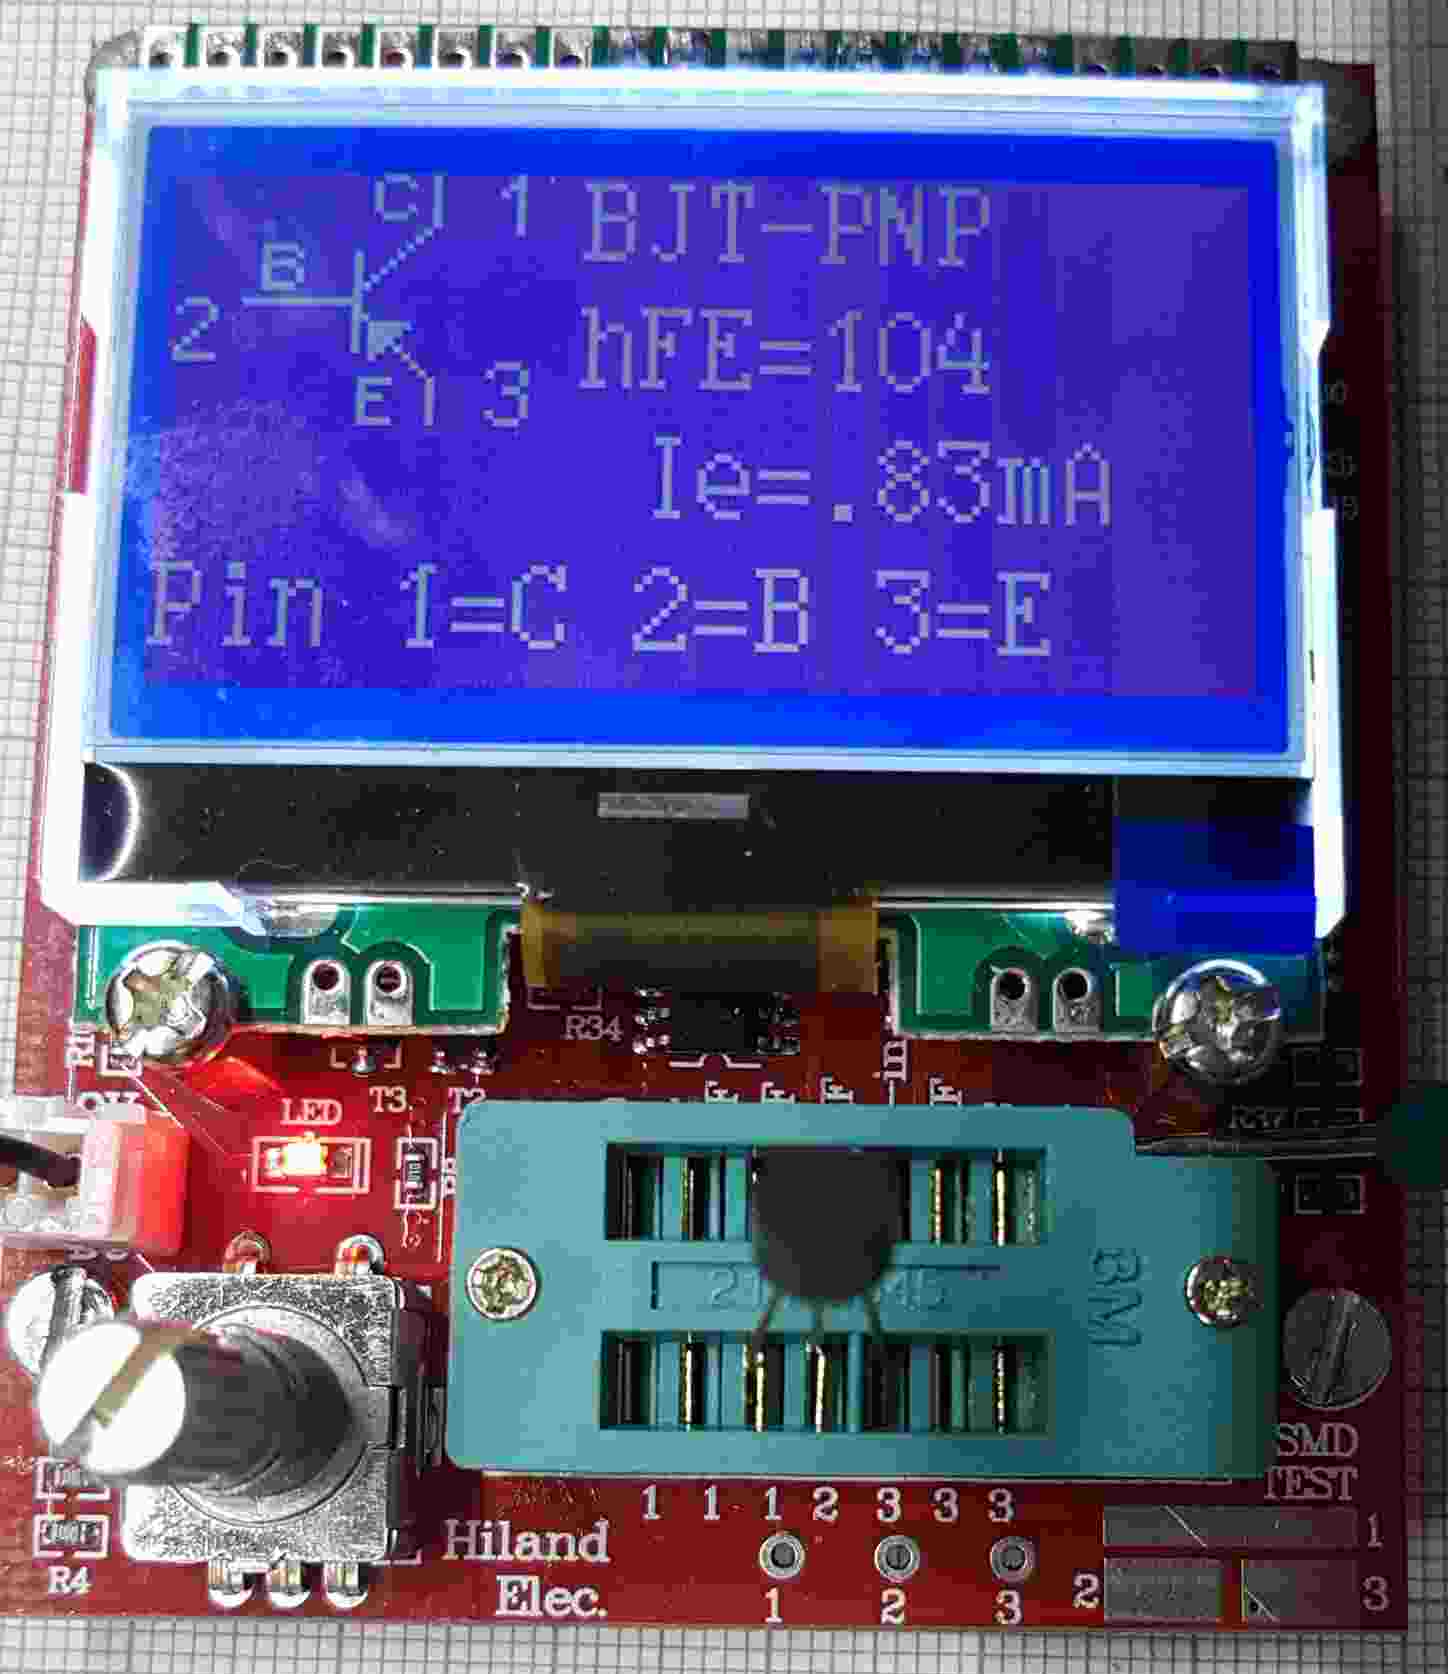
\includegraphics[width=.875\textwidth]{../PNG/Hi_u.jpg}  % width=7cm
    \caption{unten TP1 bis TP3 für Bauteilebestimmung}
  \end{subfigure}
~
  \begin{subfigure}[b]{.5\textwidth}	% 9cm
    \centering
    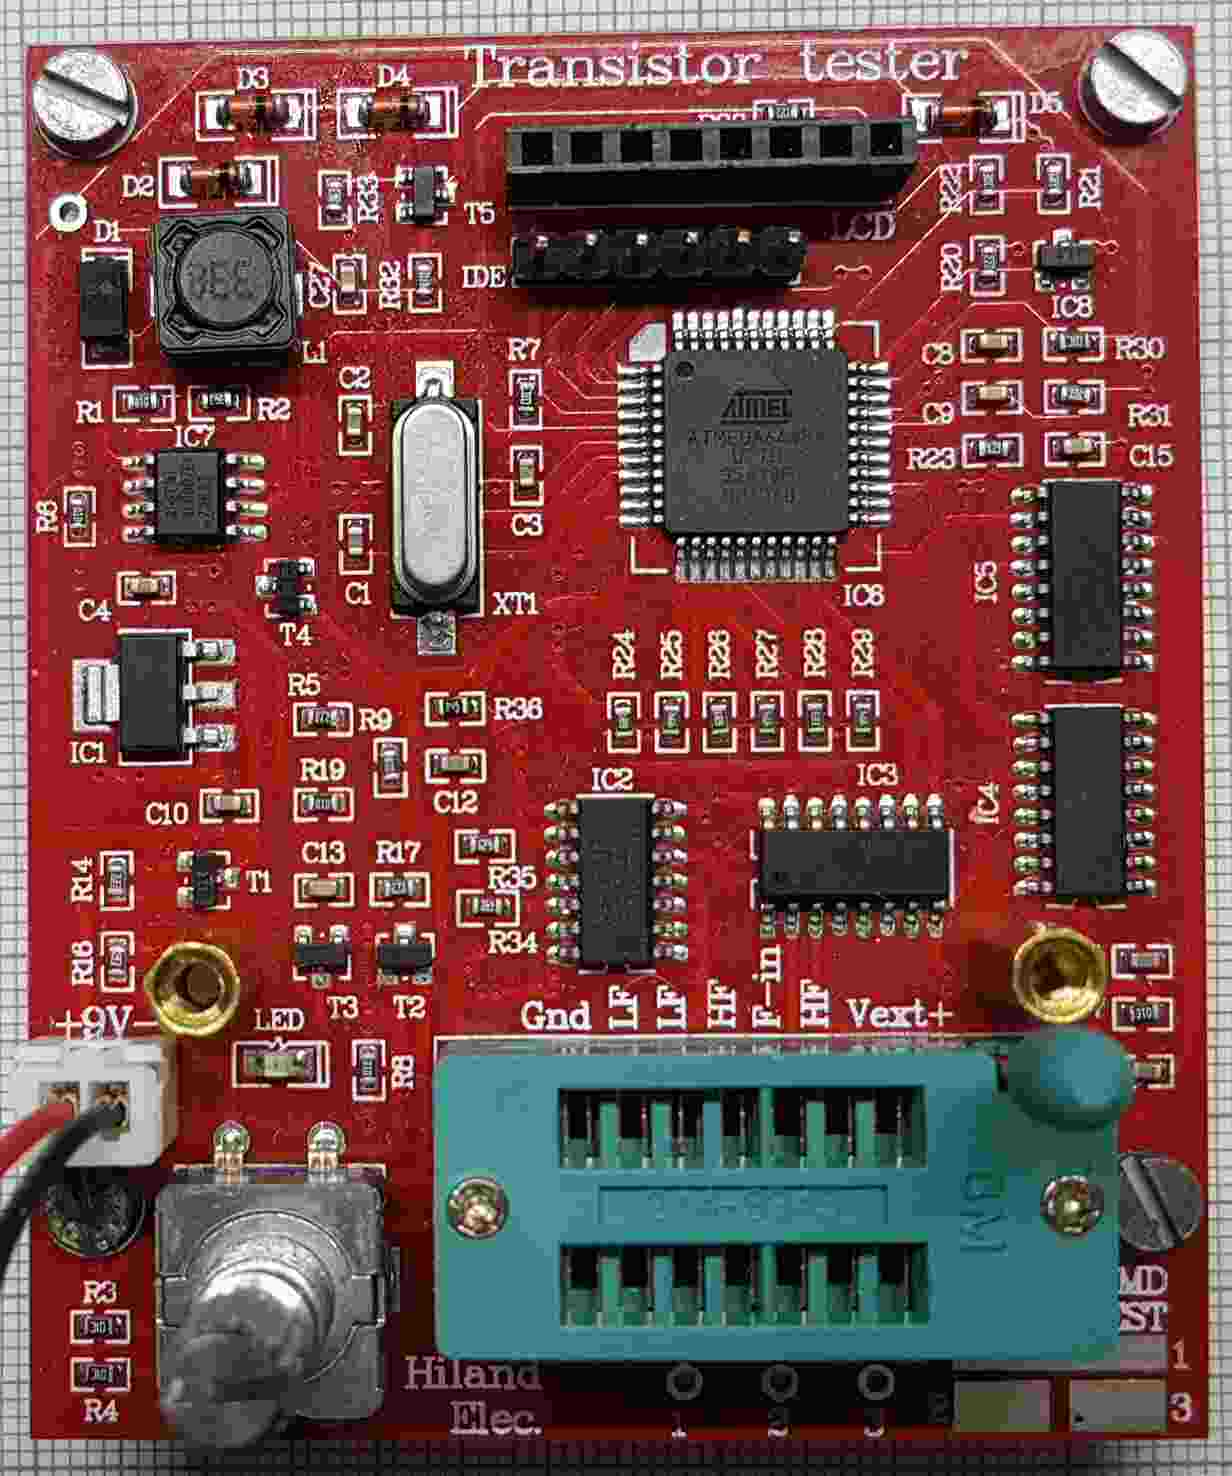
\includegraphics[width=.756\textwidth]{../PNG/Hi_o.jpg}  % 6.8cm
    \caption{oben Pins für Auswahlmenü und die IDE}
  \end{subfigure}
  \caption{Hiland Tester mit Testsockel und 128x64 Pixel Display}
\label{fig:Hiland}
\end{figure}

\textbf {Die Testports TP1, TP2 und TP3} werden für die automatische Bauteilerkennung benutzt
und sind auf der Platine mit den Ziffern \textbf {1~~1~~1~~2~~3~~3,3} gekennzeichnet.

Die gleiche Bezeichnung befindet sich auf dem SMD Testfeld
und es besteht auch eine Möglichkeit, eigene Test Kabel anzulöten.
Der \textbf {Testport TP2} wird auch für die Ausgabe der Sonderfunktion \inquotes{f-Generator} benutzt.\\
Die mit \textbf {LF} bezeichneten Pins sind für die Messung von Quarzen mit niedriger Resonanzfrequenz vorgesehen,
und die mit \textbf {HF} bezeichneten Pins sind für Quarze mit hoher Resonanzfrequenz bestimmt.

Der Pin \textbf {F-in} wird zusammen mit  \textbf {Gnd} für die Sonderfunktion Frequenz benutzt.
Und der Pin \textbf {Vext+} wird genauso mit \textbf {Gnd} für die Spannungsmessung
\textbf {und} die Zenerdiodenmessung benutzt.

\section{Fehlersuche}
Bei den meisten Problemen werden Sie den Text auf dem LCD-Display vermissen.
Zuerst sollten Sie prüfen, ob die LED auf der Platine schwach leuchtet, wenn Sie den Start-Taster
loslassen.
\begin{description}

\item[Gerät schaltet nicht ein]  
Wenn die LED nicht leuchtet, aber die VCC-Spannung den richtigen Wert hat, wenn
man den Start-Taster gedückt hält, schaltet der Mikrocontroller nicht richtig ein.
Der Mikrocontroller sollte die Spannung behalten indem der Ausgang PD6 auf \(5V\)
geschaltet wird, was üblicherweise als eine der ersten Aktionen getan wird.
Wenn man die Start-Taste gedrückt hält, bleibt die Spannung ohnehin eingeschaltet.
So können Sie mit gedrücktem Taster den Wert der VCC-Spannung und zusätzlich den Spannungswert am
Ausgang PD6 prüfen.
Wenn die VCC-Spannung den richtigen Wert (\(5V\)) hat, aber die Spannung am Ausgang
PD6 unter \(4V\) ist, startet der Mikrocontroller nicht richtig.
Für diesen Fall sollten Sie prüfen, ob die Programmdaten für den Flashspeicher
für den richtigen Prozessor-Typ ist und ob der Prozessor richtig konfiguriert ist (fuses).
Wenn der ATmega den Ausgang PD6 auf \(5V\) schaltet und die Betriebsspannung 
trotzdem nicht eingeschaltet bleibt, wenn man den Start-Taster loslässt, ist der
Grund schwieriger zu finden.
Zuerst kann man die LED kurzschliessen und es noch einmal versuchen.
Wenn der Tester jetzt startet, ist die LED möglicherweise falsch herum eingebaut.
Wenn das nicht die Ursache ist, könnte der Grund ein unzureichender Stromverstärkungs-Faktor
des Transistors T3 (BC557C) sein.
Der Strom in die Basis von T3 ist niedriger, wenn der Mikrocontroller mit der LED einschaltet
		wie im \inquotes{Taster gedrückt}-Zustand.

\item[Nichts ist lesbar auf der LCD-Anzeige] 
Prüfen Sie die Spannung am Kontrast-Pin der LCD-Anzeige (Pin 3).
Stellen Sie mit dem Trimmer den Wert auf einen im Datenblatt angegebenen Wert und optimieren Sie
durch Sichtkontrolle.
Wenn Sie ein Hochtemperatur-Display haben, brauchen Sie eine negative Kontrast-Spannung für
den Betrieb.
In diesem Fall kann man den ICL~7660-Baustein zum Erzeugen der negativen Spannung aus der
positiven \(5V\) verwenden.

Der Tester kann für viele verschiedene Controller mit unterschiedlichen Anschlußarten
konfiguriert werden. Prüfen sie auf jeden Fall, ob die Software zu ihrem Display paßt.
Wenn keine Anzeige auf dem LCD erkannt wird und wenn die Hintergrundbeleuchtung an ist,
sollten Sie die Spannungsversorgung trennen und alle vier Datenverbindungen sowie die 
beiden Steuersignale überprüfen.
Wenn alle Verbindungen in Ordnung sind, sehe ich als Ursache nur noch die Möglichkeit einer
falschen Zeitabfolge der Steuersignale.
Die Ursache hierfür kann sein, dass der LCD-Controller langsamer ist als es die Software
des ATmega erwartet. Es könnte auch sein, dass der ATmega auf der falschen Taktrate läuft.
Bitte überprüfen Sie für welche Taktrate die Software übersetzt ist und ob
die fuses des ATmega für diese Geschwindigkeit richtig gesetzt sind.
Sie finden die eingestellte Taktrate in der betreffenden Makefile.
Wenn der Tester ohne die Abschalt-Elektronik aufgebaut ist, kann man mit einer
an die Test Pins angeschlossenen LED testen, ob das Programm arbeitet.
Wenn die LED flackert, läuft das Programm. Der Fehler muss in diesen Fall an
dem Anschluss des LCD's liegen. 
Bei einigen graphischen Displays kann der Kontrast über eine Menüfunktion verstellt werden.
Wenn man hier versehentlich den Kontrast zu weit verstellt hat, ist auf dem Display
nicht mehr zu erkennen, man kann also auch nicht mehr weiter bedienen.
Hier können Sie nur versuchen, ob von der Seite (schräg) doch noch etwas zu erkennen ist
und über das Menü den Kontrast zurückstellen. Wenn dan nicht geht, können sie
das EEprom des ATmega mit einem ISP programmer neu beschreiben und damit den Kontastwert zurückstellen.
\item[Einiges, aber nicht alles ist auf der LCD-Anzeige lesbar] 
Überprüfen Sie ob die .eep-Daten in den EEPROM des ATmega geladen wurden.
Wenn alle Programmdaten richtig geladen wurden, sollten Sie die Taktrate ihrer
Programmdaten (Makefile) und die ATmega-Einstellungen prüfen (fuses).

\item[Messung ist zu langsam und Kapazitäten werden um Faktor 8 zu klein gemessen.] 
Sie betreiben die Software, die für \(8MHz\) übersetzt wurde mit einer Taktrate von \(1MHz\).
Bitte konfigurieren Sie den ATmega mit den fuses richtig.

\item[Die Messung ergibt seltsame Ergebnisse]  
Überprüfe ob der ISP-Programmierstecker noch verbunden ist.
Der ISP-Stecker sollte nicht während einer Messung eingesteckt bleiben.
Sehr oft ist der Grund für falsche Messergebnisse, dass die Software mit der
 AUTOSCALE\_ADC Option und der NO\_REF\_CAP Option übersetzt wurde, aber der
Kondensator am AREF-Pin hat immer noch einen Wert von \(100nF\).
Falsche Bestückung von Bauteilen können auch eine Ursache für Messfehler sein 
oder zurückgebliebene Flussmittelreste können die Messung stören.
Bitte prüfen Sie nach Möglichkeit mit der Selbsttest-Funktion der
TransistorTester-Software.
Zu den Einzelheiten schauen Sie in das Selbsttest-Kapitel~\ref{sec:selftest}.

Anderenfalls prüfen sie Ihre Platine visuell und prüfen Sie die Widerstandswerte
mit einem Ohmmeter. Sie können die Pins des ATmega für diese Prüfung benutzen,
zum Beispiel können Sie der Widerstand R1 zwischen Pin 23 und Pin 14 messen.
Schauen Sie in das Schaltbild~\ref{fig:ttester} für die Einzelheiten.
Man braucht den Mikrocontroller nicht zu entfernen, nur die Stromversorgung sollte
vorher getrennt werden.

\item[Der Tester schaltet nach 2 Sekunden Anzeigezeit aus]  
Dies ist dann der Fall, wenn der Pull-Up-Widerstand am PD7-Eingang
fehlt oder der Taster dauernd gedrückt wird. 
Die Software schaltet die internen Pull-Up-Widerstände ab, um eine Beeinflussung
der Messergebnisse auszuschließen. Deswegen ist ein externer Widerstand erforderlich.

\item[Der Tester zeigt immer nur Vext=xx.xV in Zeile 2 an]
Dies ist dann der Fall, wenn der Pull-Up-Widerstand am PD7 Eingang
fehlt oder der Taster dauernd gedrückt wird.
Die Software ist außerdem ohne seriellen Ausgang (ohne Option WITH\_UART) und
ohne interne Pull-Up Widerstände (mit Option PULLUP\_DISABLE) konfiguriert.
Installieren Sie einen Pull-Up Widerstand an PD7.

\end{description}


\chapter{Instructions for use}
\label{sec:manual}
\section{The measurement operation}
Using of the Transistor-Tester is simple.
Anyway some hints are required.
In most cases are wires with alligator clips connected to the test ports with plugs.
Also sockets for transistors can be connected.
In either case you can connect parts with three pins to the three test ports in any order.
If your part has only two pins, you can connect this pins to any two of the tree test ports.
Normally the polarity of part is irrelevant, you can also connect pins of electrolytical capacitors in any order. 
The measurement of capacity is normally done in a way, that the minus pole is at the test port with the lower number.
But, because the measurment voltage is only between \(0.3V\) and at most \(1.3V\), the polarity doesn\'t matter.
When the part is connected, you should not touch it during the measurement. You should put it down to a nonconducting pad
if it is not placed in a socket. You should also not touch to the isolation of wires connected with the test ports.
Otherwise the measurement results can be affected.
Then you should press the start button.
After displaying a start message, the measurement result should appear after two seconds.
If capacitors are measured, the time to result can be longer corresponding to the capacity.

How the transistor-tester continues, depends on the configuration of the software.

\begin{description}
  \item[Single measurement mode] If the tester is configured for single measurement mode (POWER\_OFF option), the tester shut off automatical 
after displaying the result for 28~seconds for a longer lifetime of battery. 
During the display time a next measurement can be started by pressing the start button.
After the shut off a next measurement can be started too of course.
The next measurement can be done with the same or another part.
If you have not installed the electronic for automatic shut down, your
last measurement result will be displayed until you start the next measurement.

  \item[Endless measurement mode] A special case is the configuration without automatical shut off.
For this case the POWER\_OFF option is not set in the Makefile.
This configuration is normally only used without the transistors for the shut off function.
A external off switch is necessary for this case. The tester will repeat measurements until power
is switched off.

  \item[Multi measurement mode] In this mode the tester will shut down not after the first measurement but 
after a configurable series of measurements.
For this condition a number (e.g.~5) is assigned to the POWER\_OFF option.
In the standard case the tester will shut down after five
measurements without found part. If any part is identified by test, the tester is shut down after double of
five (ten) measurements. A single measurement with unknown part after a series of measurement of known parts will
reset the counter of known measuerements to zero. Also a single measurement of known part will reset the counter
of unknown measurements to zero. This behavior can result in a nearly endless series of measurements without
pressing the start button, if parts are disconnected and connected in periodical manner.

In this mode there is a special feature for the display period. If the start button is pressed only short for switching
on the tester, the result of measurement ist only shown for 5 seconds. Buf if you press and hold the start button until
the first message is shown, the further measurement results are shown for 28~seconds.
The next measurement can started earlier by pressing the start button during the displaying of result.

\end{description}

\section{Optional menu functions for the ATmega328}
If the menu function is selected, the tester start a selection menu after a long key press (\textgreater~500ms)
for additional functions.
This function is also available for other processors with at least 32K flash memory.
The selectable functions are shown in row two of a 2-line display or as marked function in row 3 of a 4-line display.
The previous and next function is also shown in row 2 and 4 of the display in this case.
After a longer wait time without any interaction the program leave the menu and returns to the normal transistor tester function.
With a short key press the next selection can be shown.
A longer key press starts the shown or marked function.
After showing the last function \inquotes{switch off}, the first function will be shown next.

If your tester has also the rotary pulse encoder installed, you can call the menu with the additional functions
also with a fast rotation of the encoder during the result of a previous test is shown.
The menu functions can be selected with slow rotation of the encoder in every direction.
Starting of the selected menu function can only be done with a key press.
Within a selected function parameters can be selected with slow rotation of the encoder.
A fast rotarion of the encoder will return to the selection menu.

\begin{description} \setlength{\itemsep}{0em}
 \item[frequency]
 The additional function \inquotes{frequency} (frequency measurement) uses the ATmega Pin PD4, which is also connected to the LCD.
First the frequency is allways measured by counting.
If the measured frequency is below \(25kHz\), additionally the mean period of the input signal
is measured and with this value the frequency is computed with a resolution of up to \(0.001Hz\).
By selecting the POWER\_OFF option in the Makefile, the period of frequency measurement is limited to 8~minutes.
The frequency measurement will be finished with a key press and the selectable functions are shown again.\\

 \item[f-Generator]
 With the additional function \inquotes{f-Generator} (frequency generator) you can select output frequencies between 1Hz and 2MHz.
You can change the selected frequency only at the highest shown digit location. 
For the locations 1Hz up to 10kHz digits between 0 and 9 can be selected.
For the highest 100kHz location you can select numericals between 0 and 20.
In row 1 of the frequency line is indicated with the symbol \textgreater~~or \textless~, 
if a longer key press (\textgreater~0.8s) select a higher or lower digit location.
You can only select a lower location (\textless), if the current location has selected the 0 digit and 
if the current location is not the lowest with 1Hz steps.
If you have selected the 100kHz location, the \textgreater~symbol is replaced by a R character. 
A longer key press (\textgreater~0.8s) will result a reset of the frequency value to the initial value of 1Hz in this case.
If the POWER\_OFF option is selected in the Makefile, the key must be pressed longer, because a
short key press (\textless~0.2s) only reset the time limit of 4~minutes.
The elapsed time is shown with a point for every 30 seconds in row 1 of the display.
With periodical short key press you can prevent the time out of the frequency generation.
With a long key press (\textgreater~2s) you will stop the frequency generator and return to the function menu.\\

\item[10-bit PWM]
The additional function \inquotes{10-bit PWM} (Pulse Width Modulation) generates a fixed frequency with selectable
puls width at the pin TP2.
With a short key press (\textless~0.5s) the pulse width is increased by \(1\%\), with a longer key press the pulse width
is increased by \(10\%\).
If \(99\%\) is overstepped, \(100\%\) is subtracted from the result.
If the POWER\_OFF option is selected in the Makefile, the frequency generation is finished after 8~minutes without any key press.
The frequency generation can also be finished with a very long key press (\textgreater~1.3s).\\

\item[C+ESR@TP1:3]
The additional function \inquotes{C+ESR@TP1:3} selects a stand-alone capacity measurement with 
ESR (Equivalent Series Resistance) measurement at the test pins TP1 and TP3. 
Capacities from \(2\mu F\) up to \(50mF\) can be measured. 
Because the measurement voltage is only about \(300mV\), in most cases the capacitor can be
measured \inquotes{in circuit} without previous disassembling.
If the POWER\_OFF option is selected in the Makefile, the count of measurements is limited
to 250, but can be started immediately again.
The series of measurements can be finished with a long key press.\\

 \item[Resistor meter]
With the \mbox{1 \electricR 3} symbol the tester changes to a resistor meter at TP1 and TP3 . 
This operation mode will be marked with a \textbf{[R]} at the right side of the first display line.
Because the ESR measurement is not used in this operation mode, the resolution of the measurement
result for resistors below \(10\Omega\) is only \(0.1\Omega\).
If the resistor measurement function is configured with the additional inductance measurement,
a \mbox{1 \electricR \electricL 3} symbol is shown at this menu.
Then the resistor meter function includes the measurement of inductance for resistors below \(2100\Omega\).
At the right side of the first display line a \textbf{[RL]} is shown.
For resistors below \(10\Omega\) the ESR measurement is used,
if no inductance is find out. For this reason the resolution for resistors below \(10\Omega\) 
is increased to \(0.01\Omega\).
With this operation mode the measurement is repeated without any key press.
With a key press the tester finish this operation mode and returns to the menu.
The same resistor meter function is started automatically, if a single resistor is connected between TP1 and TP3
and the start key was pressed in the normal tester function. In this case the tester returns
from the special mode opration to the normal tester function with a key press.

 \item[Capacitor meter]
With the \mbox{\begin{large}1 \electricC 3\end{large}} symbol the tester changes to a capacitor meter function at TP1 and TP3.
This operation mode will be marked with a \textbf{[C]} at the right side of the first display line.
With this operation mode capacitors from \(1pF\) up to \(100mF\) can be measured.
In this operation mode the measurement is repeated without key press.
With a key press the tester finish this operation mode and returns to the menu.
In the same way as with resistors, the tester changes automatically to the capacitor meter function,
if a capacitor between TP1 and TP3 is measured with the normal tester function.
After a automatically start of the capacitor meter function the tester returns with a key press to
the normal tester function.

\item[rotary encoder]
With the function \inquotes{rotary encoder} a rotary encoder can be checked.
The three pins of the rotary encoder must be connected in any order to the three probes of the transistor tester 
before the start of the function. 
After starting the function the rotary knob must be turned not too fast.
If the test is finished successfully, the connection of the encoder switches  is shown symbolic in display row 2.
The tester finds out the common contact of the two switches and shows, if the indexed position has
both contacts in open state ('o') or in closed state ('C').
A rotary encoder with open switches at the indexed positions is shows in row 2 for two seconds as \inquotes{1-/-2-/-3 o}.
This type of encoder has the same count of indexed positions as count of pulses for every turn. 
Of course the pin number of the right common contact is shown in the middle instead of '2'.
If also the closed switches state is detected at the indexed positions, the row 2 of the display is also
shown as \inquotes{1---2---3 C} for two seconds.
I don't know any rotary encoder, which have the switches always closed at any indexed position.
The interim state of the switches between the indexed positions is also shown in row 2 for a short time (\textless\(~0.5s\))
without the characters 'o' or 'C'.
If you will use the rotary encoder for handling the tester, you should set the Makefile option WITH\_ROTARY\_SWITCH=2
for encoders with only the open state ('o') and set the option WITH\_ROTARY\_SWITCH=1 for encoders 
with the open ('o') and closed ('C') state at the indexed positions.\\

\item[C(\(\mu F\))-correction]
With this menu function you can change a correction factor for bigger capacity values.
You can preset the same factor with the Makefile option C\_H\_KORR.
Values above zero reduce the output value of the capacity with this percent value, values below zero will increase
the shown capacity value. A short key press will reduce the correction value about 0.1\%, a longer key press will
increase the correction value. A very long key press will save the correction value.
It is a characteristic of the used measurement method, that capacitors with low quality like electrolytic type will
result to a too high capacity value. You can detect a capacitor with low quality by a higher value of the Vloss parameter.
High quality capacitors have no Vloss or only 0.1\%.
For adjusting this parameter you should only use capacitors with high quality and a capacity value above \(50\mu F\).
By the way the exactly capacity value of electrolytic capacitors is unimportant, because the capacity value differ
with temperature and DC-voltage.

\item[Selftest]
With the menu function \inquotes{Selftest} a full selftest with calibration is done.
With that call all the test functions T1 to T7 (if not inhibited with the NO\_TEST\_T1\_T7 option) 
and also the calibration with external capacitor is done every time.\\

\item[Voltage]
The additional function \inquotes{Voltage} (Voltage measurement) is only possible, if the serial output is deselected
or the ATmega has at least 32 pins (PLCC) and one of the additional pins ADC6 or ADC7 is used for the measurement.
Because a 10:1 voltage divides is connected to PC3 (or ADC6/7), the maximum external voltage can be \(50V\).
A installed DC-DC converter for zener diode measurement can be switched on by pressing the key.
Thus connected zener diodes can be measured also.
By selecting the POWER\_OFF option in the Makefile and without key pressing, the period of voltage measurement is limited to 4~minutes.
The measurement can also be finished with a extra long key press (\textgreater~4~seconds).

\item[Contrast] 
This function is available for display controllers, which can adjust the contrast level with software.
The value can be decreased by a very short key press or left turn with the rotary encoder.
A longer key press (\textgreater~0.4s) or a right turn of the rotary encoder will increase the value.
The function will be finished and the selected value will be saved nonvolatile in the EEprom memory 
by a very long key press (\textgreater~1.3s).

\item[BackColor]
For color displays this menu item can be enabled with the Makefile option LCD\_\discretionary{}{}{}CHANGE\_\discretionary{}{}{}COLOR 
for selecting the background color. The rotary encoder extension must be installed.
You can select the colors red, green and blue with a longer key press. The intensity value of the
selected color, which is marked with a {\textgreater} symbol in column 1, can be changed by a turn of the rotary encoder.

\item[FrontColor]
For color displays this menu item can be enabled with the Makefile option LCD\_\discretionary{}{}{}CHANGE\_\discretionary{}{}{}COLOR 
for selecting the foreground color. The rotary encoder extension must be installed.
You can select the colors red, green and blue with a longer key press. The intensity value of the
selected color, which is marked with a {\textgreater} symbol in column 1, can be changed by a turn of the rotary encoder.

 \item[Show data]
 The function \inquotes{Show Data} shows besides the version number of the software the data of the calibration.
These are the zero resistance (R0) of the pin combination 1:3, 2:3 and 1:2 .
In addition the resistance of the port outputs to the \(5V\) side (RiHi) and
to the \(0V\) side (RiLo) are shown.
The zero capacity values (C0) are also shown with all pin combinations (1:3, 2:3, 1:2 and 3:1, 3:2 2:1).
Next the correction values for the comparator (REF\_C) and for the reference voltage (REF\_R) are also shown.
With graphical displays the used icons for parts and the font set is also shown.
Every page is shown for 15 seconds, but you can select the next page by a key press or a right turn of the rotary encoder.
With a left turn of the rotary encoder you can repeat the output of the last page or return to the previous page.


\item[Switch off]
With the additional function \inquotes{Switch off} the tester can be switched off immediately.\\

\item[Transistor]
Of course you can also select the function \inquotes{Transistor} (Transistor tester) to return to a normal Transistor tester measurement. 
\end{description}

With the selected POWER\_OFF option in the Makefile, all additional functions are limited in time without interaction to prevent a discharged battery.


\section{Selftest and Calibration}

If the software is configured with the selftest function, the selftest can be prepared by connecting all three
test ports together and pushing of the start button.
To begin the self test, the start butten must be pressed again within 2 seconds, or else the tester will continue
with a normal measurement.

If the self test is started, all of the documented tests in the Selftest chapter~\ref{sec:selftest} will be done.
If the tester is configured with the menu function (option WITH\_MENU), 
the full selftest with the tests T1 to T7 are only done with the \inquotes{Selftest} function, 
which is selectable as menu function.
In addition the calibration with the external capacitor is done with every call from function menu,
otherwise this part of calibration is only done first time.
Thus the calibration with the automatically started selftest (shorted probes) can be done faster.
The repetition of the tests T1 to T7 can be avoided, if the start button is hold pressed.
So you can skip uninteresting tests fast and you can watch interresting tests by releasing the start button.
The test 4 will finish only automatically if you separate the test ports (release connection).

If the function AUTO\_CAL is selected in the Makefile, 
the zero offset for the capacity measurement will be calibrated with the selftest.
It is important for the calibration task, that the connection between the three test ports is relased 
during test number 4. 
You should not touch to any of the test ports or connected cables when calibration (after test 6) is done.
But the equipment should be the same, which is used for further measurements.
Otherwise the zero offset for capacity measurement is not detected correctly.
The resistance values of port outputs are determined at the beginning of every measurement with this option.\\

If you have selected the samplingADC function in the Makefile with the option \inquotes{WITH\_SamplingADC = 1},
two special steps are included to the calibration precedure.
After the normal measuring of the zero capacity values, also the zero capacity values for the samplingADC function is
measured (C0samp). As last step of the calibration the connection of a test capacitor at pin~1 and pin~3 is requested for
later measurement of little coils with the message \mbox{\begin{large}1 \electricC 3~10-30nF[L]\end{large}}.
The capacity value should be between \(10nF\) and \(30nF\),
to get a measurable resonant frequency by later parallel connection to a coil with less than \(2mH\).
For inspection of coils with more than \(2mH\) inductance the normal measurement method should result to a
sufficient accuracy. The parallel connection of the capacitor to use the other measurement method should
not be usefull.\\

A capacitor with any capacity between \(100nF\) and \(20\mu F\) connected to pin~1 and pin~3 is
required after the measurement of the zero capacity values.
To indicate that, the message \mbox{\begin{large}1 \electricC 3~\textgreater 100nF\end{large}} is shown in row 1 of the display.
You should connect the capacitor not before the message C0= or this text is shown.
With this capacitor the offset voltage of the analog comparator will be compensated for better measurement
of capacity values.  
Additionally the gain for ADC measurements using the internal reference voltage will be adjusted too 
with the same capacitor for better resistor measurement results with the AUTOSCALE\_ADC option.
If the menu option is selected for the tester and the selftest is not started as menu function,
the calibration with the external capacitor is only done for the first time calibration.
The calibration  with the external capacitor can be repeated with a selftest call as menu selection.

The zero offset for the ESR measurement will be preset with the option ESR\_ZERO in the Makefile.
With every self test the ESR zero values for all three pin combinations are determined.
The solution for the ESR measurement is also used to get the values of resistors below \(10\Omega\) with
a resolution of \(0.01\Omega\).


\section{special using hints}
Normally the Tester shows the battery voltage with every start. If the voltage fall below a limit,
a warning is shown behind the battery voltage. If you use a rechargeable \(9V\) battery, you should replace
the battery as soon as possible or you should recharge.
If you use a tester with attached \(2.5V\) precision reference, the measured supply voltage will be shown
in display row two for 1 second with \inquotes{VCC=x.xxV}.

It can not repeat often enough, that capacitors should be discharged before measuring.
Otherwise the Tester can be damaged before the start button is pressed.
If you try to measure components in assembled condition, the equipment should be allways disconnected from power source.
Furthermore you should be sure, that no residual voltage reside in the equipment.
Every electronical equipment has capacitors inside!

If you try to measure little resistor values, you should keep the resistance of plug connectors and cables in mind.
The quality and condition of plug connectors are important, also the resistance of cables used for measurement.
The same is in force for the ESR measurement of capacitors.
With poor connection cable a ESR value of \(0.02\Omega\) can grow to \(0.61\Omega\).
If possible, you should connect the cables with the test clips steady to the tester (soldered).
Then you must not recalibrate the tester for measuring of capacitors with low capacity values,
if you measure with or without the plugged test cables. 
For the calibration of the zero resistance there is normaly a difference, if you connect the
three pins together directly at a socket or if you connect together the test clips at the end of cables.
Only in the last case the resistance of cables and clips is included in the calibration.
If you are in doubt, you should calibrate your tester with jumpers directly at the socket 
and then measure the resistance of shorten clips with the tester.

You should not expect very good accuracy of measurement results, especially the ESR measurement and the results of inductance measurement are not very exact.
You can find the results of my test series in chapter~\ref{sec:measurement} at page~\pageref{sec:measurement}.

\section{Compoments with problems}
You should keep in mind by interpreting the measurement results, that the circuit of the TransistorTester is
designed for small signal semiconductors. In normal measurement condition the measurement current can only reach about \(6mA\).
Power semiconductors often make trouble by reason of residual current with the identification an the measurement of junction capacity value.
The Tester often can not deliver enough ignition current or holding current for power Thyristors or Triacs.
So a Thyristor can be detected as NPN transistor or diode. Also it is possible, that a Thyristor or Triac is detected as unknown.

Another problem is the identification of semiconductors with integrated resistors.
So the base - emitter diode of a BU508D transistor can not be detected by reason of the parallel connected
internal \(42\Omega\) resistor.
Therefore the transistor function can not be tested also.
Problem with detection is also given with power Darlington transistors. We can find often internal
base - emitter resistors, which make it difficult to identify the component with the undersized measurement current.

\section{Measurement of PNP and NPN transistors}
For normal measurement the three pins of the transistor will be connectet in any order to the measurement
inputs of the TransistorTester.
After pushing the start button, the Tester shows in row 1 the type (NPN or PNP), 
a possible integrated protecting diode of the Collector - Emitter path and the
sequence of pins. The diode symbol is shown with correct polarity.
Row 2 shows the current amplification factor \(B\) or \(hFE\) and the current, by which the
amplification factor is measured. If the common emitter circuit is used for the hFE determinatation,
the collector current \(Ic\) is output. If the common collector circuit is used for measuring of the
amplification factor, the emitter current \(Ie\) is shown.
Further parameters are shown for displays with two lines in sequence, one after the the other in line 2.
For displays with more lines further parameters are shown directly until the last line is allready used.
When the last line is allready used before, the next parameter is shown also in the last line
after a time delay automatically or earlier after a key press.
If more parameters are present than allready shown, a + character is shown at the end of the last line.
The next shown parameter is anyway the Base - Emitter threshold voltage.
If any collector cutoff current is measurable, the collector current without base current \(I_CE0\)
and the collector current with base connected to the emitter \(I_CES\) is also shown.
If a protecting diode is mounted, the flux voltage \(Uf\) is also shown as last parameter.


With the common Emitter circuit the tester has only two alternative to select the base current:
\begin{enumerate}
\item The \(680\Omega\) resistor results to a base current of about \(6.1mA\). 
This is too high for low level transistors with high amplification factor, because the base is saturated.
Because the collector current is also measured with a \(680\Omega\) resistor, the collector current
can not reach the with the amplification factor higher value.
The software version of Markus F. has measured the Base - Emitter threshold voltage in this ciruit (Uf=...).\\
\item The \(470k\Omega\) resistor results to a base current of only \(9.2\mu A\) .
This is very low for a power transistor with low current amplification factor.
The software version of Markus F. has identified the current amplification factor with this circuit (hFE=...).\\
\end{enumerate}

The software of the Tester figure out the current amplification factor additionally with the common Collector circuit.
The higher value of both measurement methodes is reported.
The common collector circuit has the advantage, that the base current is reduced by negative current feedback corresponding
to the amplification factor. 
In most cases a better measurement current can be reached with this methode for power transistors
with the \(680\Omega\) resistor and for Darlington Transistors with \(470k\Omega\) resistor.
The reported Base - Emitter threshold voltage Uf is now measured with the same current used 
for determination of the current amplification factor.
However, if you want to know the Base - Emitter threshold voltage with a measurement current of about \(6mA\),
you have to disconnect the Collector and to start a new measurement.
With this connection, the Base - Emitter threshold voltage at \(6mA\) is reported. The capacity value
in reverse direction of the diode is also reported.
Of course you can also analyse the base - collector diode.

With Germanium transistors often a Collector cutoff current \(I_{CE0}\) with currentless base or 
a Collector residual current \(I_{CES}\) with base hold to the emitter level is measured.
Only for ATmega328 processors the Collector cutoff current is shown in this case at the row 2 of the LCD 
for 5 seconds or until the next keypress before showing the current amplification factor. 
With cooling the cutoff current can be reduced significant for Germanium transistors.


\section{Measurement of JFET and D-MOS transistors}
Because the structure of JFET type is symmetrical, the Source and Drain of this transistores can not
be differed.
Normally one of the parameter of this transistor is the current of the transistor with the Gate at the same level as Source.
This current is often higher than the current, which can be reached with the measurement circuit of the TransistorTester
with the \(680\Omega\) resistor.
For this reason the \(680\Omega\) resistor is connected to the Source. Thus the Gate get with the growing of current a negative
bias voltage.
The Tester reports the Source current of this circuit and additionally the bias voltage of the Gate.
So various models can be differed.
The D-MOS transistors (depletion type) are measured with the same methode.

\section{Measurement of E-MOS transistors and IGBTs}
You should know for enhancement MOS transistors (P-E-MOS or N-E-MOS), that the measurement of the gate threshold voltage (Vth)
is more difficult with little gate capacity values. You can get a better voltage value, if you connect a capacitor with a value
of some nF parallel to the gate /source.
The gate threshold voltage will be find out with a drain current of about \(3.5mA\) for a P-E-MOS and about \(4mA\) for a N-E-MOS.
The RDS or better R\textsubscript{DSon} of E-MOS transistors is measured with a gate - source voltage of nearly \(5V\),
which is probably not the lowest value.
In addition, the RDS resistance is determined at a low drain current, which limits the resolution of the resistance value.
Often in the case of IGBTs and sometimes also withn enhancement MOS transistors, the available \(5V\) of the tester
is not sufficient to drive the transistor across the gate.
In this case, a battery with about \(3V\) will help to make a detection and measurements with the tester possible.
The battery is connected to the gate of the transistor with one pole and the other pole of the battery
is then connected to a test port (TP) of the tester instead of the transistor gate.
When the battery is correctly polarized, the battery voltage is added to the control voltage of the tester and
the detection of the transistor succeeds.
The battery voltage must then be added to the indicated gate threshold voltage of course,
in order to get the correct threshold voltage for this component


\section{Measurement of capacitors}
The capacity values are always computed from the time constant, which is build by the serial connection of the
build in resistors with the capacitor during charging. With little capacity values the \(470k\Omega\) resistors are
used for the measurement the time to reach a threshold voltage.
For bigger capacity values with some \(10\mu F\) the voltage grow at the capacitor is monitored after charge pulses with the
\(680\Omega\) resistors. With this voltage grow the capacity can be computed together with the count of fixed length pulses.
Very low capacity values can be measured with the samplingADC method.
For analysing the same load pulse is repeated many times and the voltage is monitored with the time shift of the ADC S\&H time
using interval-tics build from the processor clock. But a complete AD conversion take 1664 processor tics!
Up to 250 ADC samples are build by this way and from the voltage curve the capacity value is computed.
If the samplingADC function is selected in the Makefile, all capacitors with less than \(100pF\) are measured with
the samplingADC function in the capacitor-meter mode \textbf{[C]}. The resolution is up to \(0.01pf\) with a clock 
frequency of \(16MHz\). The calibrated condition is difficult to build with this high resolution.
You can assume the use of the samplingADC methode every time, fractions of \(1pF\) are displayed at the screen.
By the way it should mentiored, that the junction capacitance of single diodes can also be measured with
this method. Because this method can measure the capacity value by charging or discharging, two capacity results are shown.
Both values differ be reason of the capacity diode effect.

\section{Measurement of coils}
The normal measurement of the inductance is based on the measurement of the time constant of the current grow.
The detection limit is about \(0.01mH\), if the resistance of the coil is below \(24\Omega\).
For bigger resistance values the resolution is only \(0.1mH\).
If the resistance is above \(2.1k\Omega\), this technique can never be used to detect coils.
The measurement results of this normal measurement is shown in the second line (resistance and inductance).
With the samplingADC method a resonant frequency of coils can be detected with greater inductance values.
If this effect is noticeable, the frequency and the quality factor Q of the coil is shown additionally in line 3. 

The method of resonant frequency measurement can also be used for the determination of the inductance value,
if a sufficient big capacitor mith know capacity value is connected parallel to a little inductance (\textless\(2mH\)).
With a parallel connected capacitor the normal measurement of inductance can no more operate well.
If the resonant frequency let assume a parallel connected capacitor, the inductance of the normal measurement
is not shown and the resistance value is shown in line 1.
For this resonant circuit the quality factor Q is also computed and shown behind the frequency value in line 3.
You can identify this type of measurement with the inductance value at the first position of line 2,
followed by the text \inquotes{ if } and the value of the assumed parallel capacity.
The value of this parallel capacitor can currently only be set with the calibration function (\mbox{\begin{large}1 \electricC 3~10-30nF(L)\end{large}}).

For displays with only two lines, the content for the third line is shown time-delayed in line 2.


\chapter{Programmieren des TransistorTesters}

\section{Konfigurieren des TransistorTesters}
\label{sec:config}
Die ganze Software des TransistorTesters ist im Quellcode verfügbar.
Die Übersetzung der Module wird mit einer \lname{Makefile} gesteuert. Die Entwicklung wurde
auf einem Ubuntu Linux mit den GNU-Werkzeugen (GNU toolchain, gcc version 4.5.3) durchgeführt.
Es sollte möglich sein, ohne Schwierigkeiten andere Linux-Betriebssysteme zu benutzen.
Um die übersetzen Daten in den Flash-Speicher oder den EEPROM-Speicher zu laden, wird das
Programm \lcmd{avrdude} \cite{avrdude} (Version 6.3) von der \lname{Makefile} benutzt, wenn man \lcmd{make upload} aufruft.
Das Programm \lcmd{avrdude} ist für Linux und Windows verfügbar.
Der GNU C-Kompiler wird auch von der AVR-studio-Software unter Windows oder von
der WinAVR \cite{winavr1},\cite{winavr2} Software benutzt.
Sie können die Programmdaten (.hex und .eep) auch mit anderen Programmen in den ATmega laden,
aber nur meine \lname{Makefile}-Version stellt sicher, dass die richtigen Daten in den gewählten Prozessor gelangen.
Avrdude lädt Daten nur in den ATmega, wenn die Signaturbytes des angeschlossenen ATmega gleich mit dem ausgewählten sind.
Wenn Sie die \lname{Makefile} ändern, wird die Software komplett neu übersetzt, wenn man \lcmd{make} oder
\lcmd{make upload} aufruft.
Die Software, die für einen ATmega8 übersetzt wurde, läuft nicht auf einem ATmega168.
Die Software, die für einen ATmega328 übersetzt wurde, läuft nicht auf einem ATmega168.
Eine Ausnahme bildet Software, die für einen ATmega168 übersetzt wurde. Diese Programmdateien
sind auch für einen ATmega328 brauchbar.
Seien Sie vorsichtig, wenn Sie nicht das mitgelieferte \lname{Makefile} benutzen.

Mit den entsprechenden Optionen ist die Software auch auf dem unveränderten Hardware-Entwurf von
Markus F. lauffähig (PARTNO=m8 , \textbf{keine} NO\_AREF\_CAP und \textbf{keine} PULLUP\_DISABLE Option).
Die Taktrate kann mit den fuses auch auf \(8MHz\) gestellt werden, dazu ist kein Quarz erforderlich!


Die folgenden Optionen der \lname{Makefile} sind verfügbar, um die Software für den Tester zu konfigurieren:

\begin{description} \setlength{\itemsep}{0em}
  \item[PARTNO] beschreibt den Ziel-Prozessor:\\
         m8 = ATmega8\\
         m168 or m168p = ATmega168\\
         m328 or m328p = ATmega328\\
         m644 or m644p = ATmega644\\
         m1284p        = ATmega1284\\
         m1280         = ATmega1280\\
         m2560         = ATmega2560\\
    Beispiel: PARTNO = m168

  \item[UI\_LANGUAGE] gibt die Sprache für den Tester an:\\
    LANG\_BRASIL, LANG\_CZECH, LANG\_DANISH, LANG\_DUTCH, LANG\_ENGLISH, \\
    LANG\_GERMAN, LANG\_HUNGARIAN, LANG\_ITALIAN, LANG\_LITHUANIAN, \\
    LANG\_POLISH, LANG\_RUSSIAN, LANG\_SLOVAK, LANG\_SLOVENE, \\
    LANG\_SPANISH, und LANG\_UKRAINIAN sind derzeit verfügbar.
 Für die russische und ukrainische Sprache ist ein LCD mit kyrillischem Zeichensatz erforderlich.\\
    Beispiel: UI\_LANGUAGE = LANG\_ENGLISH

  \item[LCD\_CYRILLIC] wird nur gebraucht, wenn man ein LC-Display mit kyrillischem Zeichensatz benutzt.
Die Zeichen \(\mu\) und \(\Omega\) sind im kyrillischen Zeichensatz nicht enthalten.
Wenn Sie diese Option angeben, werden beide Zeichen von der Software in das LCD geladen.
Setzen sie diese Option, wenn bei der Ausgabe falsche Zeichen anstelle von \(\mu\) oder \(\Omega\) erscheinen.\\
Beispiel: CFLAGS += -DLCD\_CYRILLIC

  \item[LCD\_DOGM] muss angegeben werden, wenn ein LCD mit ST7036-Controller (Typ DOG-M) zur Anzeige verwendet wird.
Der LCD-Kontrast wird dann mit Software-Befehlen eingestellt.
Falls sie den Kontrast zu weit verstellt haben, daß auf dem Display nichts mehr zu erkennen ist,
können sie zunächst versuchen, ob nicht bei seitlicher Sicht auf das Display doch noch etwas zu erkennen ist.
sonst muß das EEprom neu beschrieben werden, um den Kontrastwert zurückzusetzen.\\
Beispiel: CFLAGS += -DLCD\_DOGM

  \item[FOUR\_LINE\_LCD] kann bei einem 4x20-Zeichen-Display verwendet werden, um den Platz auf dem Display
besser auszunutzen. Zusätzliche Parameter, welche sonst nur kurz in Zeile 2 angezeigt werden, werden dann in
den Zeilen 3 und 4 angezeigt.
Bei grafischen Displays wird die Zahl der Zeilen aus der Displayhöhe und dem Zeilenabstand berechnet.\\
Beispiel: CFLAGS += -DFOUR\_LINE\_LCD

  \item[LCD\_LINE\_LENGTH] gibt die Anzahl der Zeichen an, die in einer Zeile dargestellt werden können.
Bei grafischen Displays wird die Anzahl der Zeichen aus der Zeichenbreite und der Displaybreite berechnet.\\
Beispiel: CFLAGS += -DLCD\_LINE\_LENGTH=20

  \item[DD\_RAM\_OFFSET] Bei einigen Text-Displays werden andere DD-RAM Startadressen für den Zeilenanfang
benutzt. Normalerweise beginnt die erste Zeile bei der DD-RAM Adresse 0. Bei einigen Displays wie TC1604
oder TC1602 beginnt die Zeile 1 aber bei der Adresse 128 (0x80).
Das kann mit dieser Option berücksichtigt werden.\\
Beispiel: CFLAGS += -DDD\_RAM\_OFFSET = 128

  \item[WITH\_LCD\_ST7565] Diese Option muss verwendet werden, wenn ein 128x64 Pixel LCD mit serieller
Schnittstelle angeschlossen ist.
Für diesen Displaytyp müssen weitere Optionen gesetzt werden, die in Tabelle~\ref{tab:cod-display} 
beschrieben werden.
Anstelle des ST7565-Controllers kann auch zum Beispiel der ähnliche SSD1306-Controller konfiguriert werden.
Dafür muss diese Option auf 1306 gesetzt werden.
Ein PCF8812 oder PCF8814 Controller wird ebenfalls unterstützt, wenn diese Option richtig gesetzt wird.
Auch ein Display mit ST7920 oder NT7108 Controller kann angeschlossen werden.
Für den NT7108 Controller muß ein
zusätzlicher Seriell-Parallel Wandler 74HC(T)164 oder 74HC(T)595 verwendet werden.\\
Beispiel: WITH\_LCD\_ST7565 = 1 

 \item[LCD\_INTERFACE\_MODE] Beim SSD1306-Controller kann anstelle des Standard-SPI (4-Wire) Interface auch das
I\textsuperscript{2}C-Interface benutzt werden. Dafür muss diese Option auf 2 gesetzt werden.
Für den ST7920 Controller kann ein spezieller serieller Anschluß mit dem Setzen dieser Option auf 5
unterstützt werden.
Wenn nur eine Anschlußmöglichkeit vorgesehen ist, braucht die Konstante LCD\_INTERFACE\_MODE nicht gesetzt werden.
Alle bisher möglichen Werte für LCD\_INTERFACE\_MODE und WITH\_LCD\_ST7565 sind in Tabelle~\ref{tab:cod-display} aufgeführt.\\

\begin{table}[H]
  \begin{center}
    \begin{tabular}{| c | c | c | c|}
    \hline
 Display-Typ        &  Interface     & WITH\_LCD\_ST7565 &  LCD\_INTERFACE\_MODE \\
    \hline
    \hline
  Character 16x2,   & 4-Bit parallel &  disabled (0)      & disabled (1) \\
  Character 20x4    & 4-Wire SPI     &                    &    4   \\
                  & I\textsuperscript{2}C &               &    2   \\
    \hline
  Graphic ST7565    & 4-Wire SPI      & 1 or 7565          & disabled (4) \\
    \hline
  Graphic ST7565  & I\textsuperscript{2}C & 1 or 7565     &   2 \\
    \hline
  Graphic SSD1306   & 4-Wire SPI      & 1306               & disabled (4) \\
    \hline
  Graphic SSD1306 & I\textsuperscript{2}C & 1306          &   2 \\
    \hline
  Graphic ST7920    & 4-Bit parallel  & 7920              & disabled (1) \\
    \hline
  Graphic ST7920    & 2-Bit serial    & 7920               &  5 \\
    \hline
  Graphic NT7108    & 8-Bit parallel  & 7108              & disabled (6) \\
  oder KS0108       &    + 74HCT164   &                   &      \\
    \hline
  Graphic PCF8812   & 4-Wire SPI      & 8812              & disabled (4) \\
    \hline
  Graphic PCF8814   & 4-Wire SPI      & 8814              & disabled (4) \\
                  & I\textsuperscript{2}C & 8814          &   2 \\
                    & 3-line          & 8814              &   3 \\
    \hline
  Graphic ILI9163   & 4-Wire SPI      & 9163              & disabled (4) \\
  128x128 Color     &                 &                   &              \\
    \hline
  Graphic ST7735    & 4-Wire SPI      & 7735              & disabled (4) \\
  128x160 Color     &                 &                   &              \\
    \hline
    \end{tabular}
  \end{center}
  \caption{Kennzahlen für Controller und  Art der Schnittstelle}
  \label{tab:cod-display}
\end{table}

Die Werte in Klammern werden nur Software intern benutzt und sind hier nur zur Information genannt.
Man sollte die Werte in den Klammern nicht hier in der \lname{Makefile} setzen.\\
Beispiel: CFLAGS += -DLCD\_INTERFACE\_MODE=2

  \item[LCD\_SPI\_OPEN\_COL] Mit der Option LCD\_SPI\_OPEN\_COL werden die Datensignale der SPI-Schnittstelle
nicht nach VCC direkt geschaltet.
Die Signale werden nur nach GND geschaltet, für die \inquotes{high} Signale werden die \inquotes{Pull-Up} Widerstände
des ATmega benutzt.
Für das Signal \inquotes{Reset} wird aber ein externer Pull-Up Widerstand benötigt, wenn die Option PULLUP\_DISABLE
gesetzt ist. Für die anderen SPI Signale werden die internen Pull-Up Widerstände vorübergehend benutzt,
wenn die Option PULLUP\_DISABLE gesetzt ist.
Beispiel: CFLAG += -DLCD\_SPI\_OPEN\_COL

 \item[LCD\_I2C\_ADDR] Die I\textsuperscript{2}C-Adresse des SSD1306-Controllers kann durch Vorbesetzen der Adresse LCD\_I2C\_ADDR
auf 0x3D geändert werden.\\
Beispiel: CFLAGS += -DLCD\_I2C\_ADDR=0x3d

  \item[LCD\_ST7565\_RESISTOR\_RATIO] Mit dieser Option wird das Widerstands-Teilerverhältnis für den
Spannungsregler des ST7565-Controllers eingestellt. Brauchbare Werte liegen im Allgemeinen zwischen 4 und 7.
Einstellbar sind Werte zwischen 0 und 7.\\
Beispiel: LCD\_ST7564\_RESISTOR\_RATIO = 4

  \item[LCD\_ST7565\_H\_FLIP] Mit dieser Option kann die Anzeige horizontal umgedreht werden.\\
Beispiel: CFLAGS += LCD\_ST7565\_H\_FLIP = 1

  \item[LCD\_ST7565\_H\_OFFSET] Diese Option kann den für die Ausgabe benutzten Speicher an das Anzeigefenster des
 Displays anpassen. Der Controller benutzt mehr horizontale Pixel (132) als angezeigt (128) werden.
 Ein Wert von 0, 2 oder 4 kann je nach verwendetem Display-Modul für eine korrekte Darstellung notwendig sein.\\
Beispiel: CFLAGS += LCD\_ST7565\_H\_OFFSET = 4

  \item[LCD\_ST7565\_V\_FLIP] Mit dieser Option kann die Anzeige vertikal umgedreht werden.\\
Beispiel: CFLAGS += LCD\_ST7565\_V\_FLIP = 1

  \item[VOLUME\_VALUE] Hier kann man den Kontrastwert für ST7565 oder SSD1306 Controller voreinstellen.
Der Wert kann für den ST7565 Controller zwischen 0 und 63 liegen.
Für den SSD1306 Controller sind Werte zwischen 0 und 255 erlaubt.\\
Beispiel: CFLAGS += -DVOLUME\_VALUE = 25

  \item[LCD\_ST7565\_Y\_START] Mit dieser Option kann die erste Zeile vertikal richtig gesetzt werden.
Bei einigen Display-Varianten ist die erste Zeile in die Bildmitte verschoben.
Bei diesen Displays wird die erste Zeile wieder an den oberen Rand verschoben, 
wenn diese Option auf 32 (halbe Bilschirmhöhe) gesetzt wird.\\
Beispiel: CFLAGS += -DLCD\_ST7565\_Y\_START = 32

  \item[LCD\_CHANGE\_COLOR] Diese Option erweitert die Menüfunktionen um die Möglichkeit,
die Hindergrundfarbe und die Vordergrundfarbe wählen zu können. Wenn die Option auf
den Wert 2 gesetzt wird, werden die Farben blau und rot vertauscht.
Diese Option kann nur für Farbdisplays (Controller ST7735 oder ILI9193) gewählt werden.\\
Beispiel: CFLAGS += -DLCD\_CHANGE\_COLOR=1

 \item[LCD\_BG\_COLOR] Mit dieser 16-Bit Zahl kann eine Farbe für den Hintergrund gewählt werden.
Normalerweise sind die oberen 5 Bit für die Farbe rot, die mittleren 6 Bit für die Farbe grün
und die unteren 5 Bit für die Farbe blau vorgesehen. Manchmal sind aber die Bits für die Farben 
rot und blau vertauscht.
Diese Option kann nur für Farbdisplays (Controller ST7735 oder ILI9193) gewählt werden.\\
Beispiel: CFLAGS += -DLCD\_BG\_COLOR=0x000f

 \item[LCD\_FG\_COLOR] Mit dieser 16-Bit Zahl kann eine Farbe für den Vordergrund gewählt werden.
Das Beispiel wählt weiss als Farbe für Text und Symbole aus.
Diese Option kann nur für Farbdisplays (Controller ST7735 oder ILI9193) gewählt werden.\\
Beispiel: CFLAGS += -DLCD\_FG\_COLOR=0xffff

  \item[FONT\_8X16] Für den ST7565 controller sollte ein Font ausgewählt werden.
Auswählbar sind die Fonts mit der Variablen FONT\_ mit angehängter Größe (Breite x Höhe).
iDerzeit sind 6X8, 8X8, 7X12, 8X12, 8X12thin, 8X14 8X15, 8X16 und 8X16thin.
Die Fontgröße 8x16 oder 8X16thin ist die effizienteste Wahl für das graphische 128x64-LCD.\\
Beispiel: CFLAGS += FONT\_8X16

 \item[BIG\_TP] Die Pinnummern bei der graphischen Darstellung können mit dieser Option größer dargestellt werden.\\
Beispiel: CFLAGS += BIG\_TP

 \item[INVERSE\_TP] Mit dieser Option werden die Pinnummern in der graphischen Darstellung invers (schwarz auf weiß) dargestellt.
Weil für die Darstellung ein Rand benötigt wird, kann diese Option nicht mit der Option BIG\_TP kombiniert werden.\\
Beispiel: CFLAGS += INVERSE\_TP

  \item[STRIP\_GRID\_BOARD] Diese Option passt die Software an eine andere Pinbelegung von Port~D für Streifenleiterplatinen an.
Die Einzelheiten findet man im Hardwarekapitel \ref{sec:hardware} auf Seite~\pageref{sec:hardware}.
Mit dieser Option werden auch alternative Belegungen der ATmega Pins für graphische Displays gewählt.
Für die chinesische \inquotes{T5} Platine muß die Option STRIP\_GRID\_BOARD auf 5 gesetzt werden.
Bei den Alternativen für die graphischen Displays bleibt die Belegung  des Tastensignals unverändert.\\
Beispiel: CFLAGS += -DSTRIP\_GRID\_BOARD

  \item[WITH\_MENU] aktiviert eine Menüfunktion für einen ATmega328. Man kann einige Zusatzfunktionen über ein
Auswahlmenü benutzen, welches man über einen langen Tastendruck (\textgreater~0,5s) erreichen kann.
Wenn die Menüfunktion eingeschaltet ist, wird beim automatischen Selbsttest-Start mit kurzgeschlossenen Testpins
 nur der Kalibrationsteil des Selbsttests ausgeführt.
Die Tests T1-T7 werden nur beim Selbsttest ausgeführt, der als Menüfunktion ausgewählt werden kann.\\
Beispiel: CFLAGS += -DWITH\_MENU

 \item[MAX\_MENU\_LINES]
Diese Option gibt eine maximale Zeilenzahl für die gezeigte Auswahl der Menüfunktionen an.
Normalerweise ergibt sich die Zahl der Zeilen über die vorhandene Zeilenzahl des Displays.
Da normalerweise mehr Funktionen ausgewählt werden können als auf dem Display Zeilen zur Verfügung stehen,
wird die Auswahl zyklisch ausgetauscht.
Die Aufbereitung des Displayinhalts bei dem zyklischen Austausch braucht speziell bei großen Farbdisplays
mit vielen Zeilen erhebliche Zeit.
Durch die Begrenzung der Zeilenzahl mit dieser Option kann die Ausgabezeit bei der Menüauswahl deutlich reduziert werden
und so die Bedienung beschleunigt werden.
Der Wert für diese Option ist mit 5 vorbesetzt.\\
Beispiel: CFLAGS += -DMAX\_MENU\_LINES=3

  \item[WITH\_ROTARY\_SWITCH] Die Menüfunktion kann leicher bedient werden, wenn ein Impulsdrehgeber als Erweiterung
benutzt wird.
Für die Details der notwendigen Erweiterung sehen Sie bitte die Beschreibung~\ref{fig:RotExt} im Hardwarekapitel.
Wenn der Impulsdrehgeber die gleiche Anzahl von Raststellungen wie Impulse für jede Umdrehung hat,
muss die Option WITH\_ROTARY\_SWITCH auf 2 gesetzt werden.
Wenn der Impulsdrehgeber doppelt so viele Raststellungen hat, muss die Option WITH\_ROTARY\_SWITCH auf 1 gesetzt werden.
Das Setzen der Option WITH\_ROTARY\_SWITCH auf 5 wählt die höchste Auflösung für den Impulsdrehgeber.
Jeder Zyklus der beiden Schalter-Zustände wird als 4 gezählt. Normalerweise ist diese Einstellung nur für
Impulsdrehgeber ohne Raststellung sinnvoll.
Ein Setzen der Option WITH\_ROTARY\_SWITCH auf 4 ist notwendig für die korrekte Behandlung von zwei separaten
Rauf (Up) und Runter (Down) Tastern, die anstelle der beiden Schalter eines Impulsdrehgebers eingebaut sind.
Verwenden Sie nicht die Einstellung 4 mit normalen Impulsdrehgebern!\\
Beispiel: CFLAGS += -DWITH\_ROTARY\_SWITCH=1

  \item[CHANGE\_ROTARY\_DIRECTION] Man kann die erkannte Drehrichtung des Impulsdrehgebers durch Vertauschen
der beiden Schalter-Signale oder durch Setzen dieser Option ändern.
Beispiel: CFLAGS += -DCHANGE\_ROTARY\_DIRECTION

 \item[WITH\_SELFTEST] Wenn Sie diese Option angeben, baut die Software eine Selbsttest-Funktion ein, die gestartet wird
wenn Sie alle drei Prüfspitzen verbinden und eine Messung starten.\\
Beispiel: CFLAGS += -DWITH\_SELFTEST

  \item[NO\_COMMON\_COLLECTOR\_HFE] verhindert die hFE-Messung von Transistoren in der Kollektorschaltung.
So können Sie Speicher sparen, um die erweiterten Selbsttest-Routinen T1 bis T7 für den ATmega168-Prozessor zu ermöglichen.
Standardmäßig sind beide Schaltungen für die hFE-Messung eingeschaltet,
aber dann ist kein Platz im Programmspeicher des ATmega168 für die erweiterten Selbsttests.\\
Beispiel: CFLAGS += -DNO\_COMMON\_COLLECTOR\_HFE

  \item[NO\_COMMON\_EMITTER\_HFE] schaltet die hFE-Messung von Transistoren in Emitterschaltung ab.
So können Sie Speicher sparen, um die erweiterten Selbsttest-Routinen T1 bis T7 für den ATmega168-Prozessor zu ermöglichen.
Standardmäßig sind beide Schaltungen für die hFE-Messung eingeschaltet,
aber dann ist kein Platz im Programmspeicher des ATmega168 für die erweiterten Selbsttests.\\
Beispiel: CFLAGS += -DNO\_COMMON\_EMITTER\_HFE

  \item[NO\_TEST\_T1\_T7] Diese Option verhindert die Ausführung der Selbsttest Teile T1 bis T7.
Diese Tests sind nützlich um Fehler in der Schaltung wie falsche Messwiderstände oder Isolationsprobleme zu finden.
Wenn Ihre Schaltung fehlerfrei ist, können Sie die Selbsttest-Teile T1 bis T7 durch das Setzen dieser Option weglassen, um eine
schnellere Kalibration zu erreichen.
Bei eingeschalteter Menüfunktion werden die Selbsttest-Teile T1 bis T7 nur bei Aufruf der Menüfunktion \inquotes{Selbsttest} ausgeführt.
Der ATmega168-Prozessor benutzt die Selbsttest Teile T1 bis T7 nicht, wenn beide Messmethoden für die hFE-Bestimmung benutzt werden.\\
Beispiel: CFLAGS += -DNO\_TEST\_T1\_T7

  \item[AUTO\_CAL] Der Nullabgleich für die Kondensatormessung wird beim
Selbsttest zusätzlich ins EEPROM geschrieben und ist damit für die weiteren Messungen abgeglichen.
Wenn nach dem Nullabgleich der Kondensatormessung ein Kondensator mit einer Kapazität zwischen \(100nF\) und \(20\mu F\) an Pin~1 und Pin~3 
angeschlossen wird, wird auch der Offset des analogen Komparators und die Skalierung für die AUTOSCALE\_ADC
Umschaltung auf die interne Spannungsreferenz ermittelt und ins EEPROM geschrieben.
Die Port-Ausgangswiderstände werden zu Beginn jeder Messung neu bestimmt. \\
Beispiel: CFLAGS += -DAUTO\_CAL

  \item[SHORT\_UNCAL\_MSG] Bei Prozessoren mit mindestens 32K Flash  wird nach einem Bauteiletest ein Hinweis auf einen unkalibrierten Zustand
des Testers gegeben. Normalerweise folgt dann eine kurze Anleitung, wie die Kalibration durchzuführen ist.
Diese Anleitung wird nicht ausgegeben, wenn die Option SHORT\_UNCAL\_MSG gesetzt wird.
Dann bleibt es bei einem einzeiligen Hinweis auf den unkalibrierten Zustand. 
Dies spart einerseits etwas Platz in Flash-Speicher und andererseits Ausgabezeit für Benutzer,
die ohnehin wissen, wie kalibriert wird.\\
Beispiel: CFLAGS += -DSHORT\_UNCAL\_MSG

 \item[NO\_ICONS\_DEMO]
Diese Option schaltet die zusätzliche Demonstration der Symbole und die Ausgabe des Zeichensatzes bei der Menüfunktion
\inquotes{Zeige Daten} ab.
Dies spart Platz im Flash-Speicher und auch Ausgabezeit für den Nutzer.\\
Beispiel: CFLAGS += -DNO\_ICONS\_DEMO

 \item[WITH\_ROTARY\_CHECK]
Diese Option schaltet die zusätzliche Menüfunktion für den Test eines Impulsdrehgebers frei.
Dieser Test testet einen Impulsdrehgeber, der an TP1,TP2 und TP3 angeschlossen wird.
Bitte beachten Sie, daß nicht der eingebaute Impulsdrehgeber des Testers getestet wird!
Aber ein solcher Impulsdrehgeber kann mit der Option WITH\_ROTARY\_SWITCH auch zur Bedienung des Testers eingesetzt werden.\\
Beispiel: CFLAGS += -DWITH\_ROTARY\_CHECK

 \item[NO\_FREQ\_COUNTER]
Mit dieser Option wird die Frequenzzähler Funktion des Testers abgewählt.
Dies ist besonders dann sinnvoll, wenn der benutzte Pin PD4 (ATmega328) nicht zusammen mit
dem Anschluß des Displays benutzt werden kann.
Der entsprechende Eintrag in der Liste der Menüfunktionen erscheint dann nicht mehr und es
wird auch Flash-Speicherplatz gespart.\\
Beispiel: CFLAGS += -DNO\_FREQ\_COUNTER

 \item[WITH\_FREQUENCY\_DIVIDER]
Mit dieser Option wird das Menü um einen einstellbaren Vorteiler für den Frequenzzähler erweitert.
Das Teilerverhältnis kann auf 1:1, 1:2, 1:4, 1:8, 1:16, 1:32, 1:64 und 1:128 eingestellt werden.
Diese Option ist nur sinnvoll, wenn an den Frequenzeingang ein externer Vorteiler angeschlossen wird.
Die bei der Messung angezeigten Frequenzen und Perioden berücksichtigen das eingestellte Teilerverhältnis.\\
Beispiel: CFLAGS += -DWITH\_FREQUENCY\_DIVIDER

 \item[NO\_FREQUENCY\_SWITCH]
Mit dieser Option wird die Umschaltung des Frequenzeingangs der ATmega644/ATmega1284 Schaltung nicht unterstützt.
Die LF- und HF-Quarz Messung wird mit dieser Option nicht unterstützt.\\
Beispiel: CFLAGS += -DNO\_FREQUENCY\_SWITCH=1

\item[PWM\_SERVO] 
wählt eine spezielle PWM Erzeugung zum Testen von Modellbau Servos anstelle der allgemeinen PWM Erzeugung.\\
Beispiel: CFLAGS += -DPWM\_SERVO=1

  \item[WITH\_SamplingADC] Mit dieser Funktion wird in bestimmten Fällen die Sampling-Methode für den ADC angewendet.
Durch Verschieben der Abtastzeit des ADC kann für wiederholbare Signale die Signalform mit einem Zeitabstand
von einem Prozessortakt oder auch 4 oder 16 Prozessortakte abgetastet werden. Dadurch kann die Ladefunktion von
Kondensatoren unter \(100pF\) so vermessen werden, daß sich eine Auflösung von \(0.01pF\) bei \(16MHz\) Prozessortakt ergibt.
Mit den gleichen Methode kann die Schwingfrequenz bei kleinen Spulen unter \(2mH\) mit einem parallelgeschalteten
Kondensator gemessen werden. Wenn die Kapazität des Parallel-Kondensators bekannt ist, kann die Induktivität aus
der Schwingfrequenz mit hoher Auflösung bestimmt werden. Als Nebenprodukt kann auch die Güte der Spule aus dem
Schwingverhalten geschätzt werden. Freigeschaltet werden diese Funktionen mit der Option WITH\_SamplingADC.
Bei der Kalibration werden dann sowohl zusätzlich die Nullkapazitäten mit der Samplingmethode zusätzlich bestimmt,
als auch die Kapazität eines Parallel-Kondensators vermessen für die spätere Bildung eines Schwingkreises mit einer unbekannten Spule.\\
Beispiel: WITH\_SamplingADC = 1

  \item[WITH\_XTAL]
Diese Option schaltet zusätzlich Tests für Quarze und Resonatoren frei, wenn die SamplingADC Funktion schon vorhanden ist
und ein 16 MHz Quarz verwendet wird (OP\_MHZ = 16).
Wenn möglich, werden die Frequenzen für Serien- und Parallel-Schaltung bestimmt und dann versucht,
aus dem Frequenzversatz die Serienkapazität Cm zu bestimmen.\\
Beispiel: CFLAGS += -DWITH\_XTAL

  \item[WITH\_UJT]
Diese Option schaltet zusätzliche Tests für Unijunctiontransistoren frei. 
Wenn die SamplingADC Funktion freigeschaltet wurde, wird die Schwingfähigkeit des Bauteils untersucht.
Richtig erkannt wird das Bauteil aber auch ohne die SamplingADC Funktion. 
Ohne die Option WITH\_UJT werden Unijunctiontransistoren als Doppeldiode erkannt.\\
Beispiel: CFLAGS += -DWITH\_UJT

  \item[WITH\_PUT]
  Diese Option schaltet einen zusätzlichen Test auf \inquotes{Programmable Unijunction Transistor} frei.
Ohne den zusätzlichen Test werden PUTs normalerweise als Bipolartransistor (Bipolar Junction Transistor) erkannt.\\
Beispiel: CFLAGS += -DWITH\_PUT

 \item[FET\_Idss]
Diese Option bewirkt zusätzliche Messungen, um den Drain-Strom Idss zu berechnen, wenn die Schätzung nicht
über \(60mA\) liegt. Die Schätzung und Berechnung wird mit einem angenommenen quadratischen Stromverlauf durchgeführt.
Beispiel: CFLAGS += -DFET\_Idss

  \item[FREQUENCY\_50HZ] Zum Ende des Selbsttests wird bis zu einer Minute lang ein \(50Hz\)-Signal auf Port 2 und Port 3 erzeugt.
Diese Option sollte nur in Ausnahmefällen bebraucht werden.\\
Beispiel: CFLAGS += -DFREQUENCY\_50HZ

  \item[CAP\_EMPTY\_LEVEL] Diese Option legt die Spannung (mV) für einen entladenen Kondensator fest.
  Der Wert kann höher als 3mV gesetzt werden, wenn die Entladung nicht zum Ende kommt. In diesen Fall meldet der Tester nach längerer Zeit \inquotes{Cell!}.\\
Beispiel: CFLAGS += -DCAP\_EMPTY\_LEVEL=3

  \item[WITH\_AUTO\_REF] Mit dieser Option wird die Referenzspannung gemessen, um den aktuellen Faktor für die Kapazitätsmessung 
von kleineren Kapazitäten (unter \(40\mu F\)) zu ermitteln.\\
Beispiel: CFLAGS += -DWITH\_AUTO\_REF

  \item[REF\_C\_KORR] gibt einen Offset für die gelesene Referenz-Spannung in mV-Einheiten an.
Das kann benutzt werden, um die Kapazitätsmessung kleiner Kondensatoren abzugleichen.
Wenn zusätzlich die AUTO\_CAL-Option gewählt wurde, ist diese Angabe nur ein zusätzlicher Offset für
den gefundenen Komparator-Offset.
Ein Wert von 10 ergibt etwa 1~Prozent kleinere Messergebnisse.\\
Beispiel: CFLAGS += -DREF\_C\_KORR=14

  \item[REF\_L\_KORR] gibt einen zusätzlichen Offset für die Referenz-Spannung für die Induktivitätsmessung
in mV-Einheiten an. Der REF\_C\_KORR-Offset beziehungsweise der gefundene Offset bei der Kalibration
wird bei der Induktivitätsmessung ebenfalls berücksichtigt.\\
Der REF\_L\_KORR Wert wird für die Messungen ohne \(680\Omega\) Widerstand subtrahiert, bei Messungen mit einem
\(680\Omega\) Widerstand wird der Wert addiert.
Ein Wert von 10 führt zu einer Änderung des Ergebnisses um 1 Prozent.\\
Beispiel: CFLAGS += -DREF\_L\_KORR=40

  \item[C\_H\_KORR] gibt eine Korrektur der Messergebnisse für grosse Kondensatoren an.
Eine Eingabe von 10 führt zu 1~Prozent kleineren Messergebnissen.\\
Beispiel: CFLAGS += -DC\_H\_KORR=10

  \item[WITH\_UART] benutzt den Pin PC3 zur Ausgabe der seriellen Texte (V24). Wenn die Option nicht
benutzt wird, kann der PC3 Pin zum Anschluss einer externen Spannung mit einem 10:1-Widerstandsteiler benutzt
werden. Damit können beispielsweise Zenerdioden mit höherer Durchbruchspannung getestet werden.
Diese Messung wird so lange mit etwa 3 Messungen pro Sekunde wiederholt, solange der Starttaster gedrückt bleibt.\\
Beispiel: CFLAGS += -DWITH\_UART

 \item[WITH\_HARDWARE\_SERIAL] wird nur für die serielle Ausgabe bei Testern benutzt, die mit einer Arduino UNO Platine gebaut wurden.\\
Example:  CFLAGS += -DWITH\_HARDWARE\_SERIAL

  \item[TQFP\_ADC6] Die Option TQFP\_ADC6 benutzt anstelle des PC3-Pins (ADC3) den zusätzlichen ADC-Eingang ADC6
des ATmegas im TQFP-Gehäuse oder QFN-Gehäuse.
Dadurch kann dieser Eingang unabhängig von der seriellen Ausgabe auf dem PC3 Pin genutzt werden. Dieser Pin wird
dann für die Zenerdioden-Messung und für die Messung einer externen Spannung über den Dialog des ATmega328 genutzt.\\
Beispiel: CFLAGS += -DTQFP\_ADC6

  \item[TQFP\_ADC7] Die Option TQFP\_ADC7 benutzt anstelle des PC3-Pins (ADC3) den zusätzlichen ADC-Eingang ADC7
des ATmegas im TQFP-Gehäuse und QFN-Gehäuse.
Dadurch kann dieser Pin unabhängig von der seriellen Ausgabe auf den PC3 Pin genutzt werden. Wenn diese Option 
ohne die Option TQFP\_ADC6 genutzt wird, erfolgt sowohl die Zenerdioden-Messung als auch die Messung einer externen
Spannung über den Dialog des ATmega328 genutzt. Wenn die Option zusätzlich zur TQFP\_ADC6-Option gesetzt wird,
erfolgt die Zenerdioden-Messung mit dem ADC6-Pin und bei der über den Dialog wählbaren Spannungsmessung werden
beide Eingänge gemessen. Beide Pinne sollten dann an einen 10:1-Spannungsteiler angeschlossen sein.\\
Beispiel: CFLAGS += -DTQFP\_ADC7

  \item[WITH\_VEXT] ermöglicht die Messung einer externen Spannung über einen 10:1-Spannungsteiler.
Für den ATmega168 oder ATmega328 wird normalerweise der PC3-Pin benutzt, wenn keine Option TQFP\_ADC6 oder
TQFP\_ADC7 gesetzt ist. Dann ist diese Option aber nur möglich, wenn die WITH\_UART Option nicht gesetzt ist.\\
Beispiel: CFLAGS += -DWITH\_VEXT 

  \item[RMETER\_WITH\_L] wählt für die Widerstandsmeßfunktion, die durch einen Widerstand an TP1 und TP3 gestartet wird,
zusätzlich die Messung von Induktivitäten. Der Betriebsmodus wird dann durch ein \textbf{[RL]} am Ende der ersten Displayzeile
angezeigt. Durch den zusätzlichen Test auf Induktivität wird die Meßzeit für Widerstände unter \(2100\Omega\) deutlich
länger. Ohne diese Option werden außerdem Widerstände unter \(10\Omega\) nicht mit der ESR-Methode gemessen,
da als Bauteil eine Induktivität nicht ausgeschlossen werden kann.
Wegen der kurzen Strompulse können mit der ESR-Methode keine Induktivitäten gemessen werden.
Weil nur mit der ESR-Methode eine Auflösung von \(0.01\Omega\) erreicht wird, beträgt ohne diese Option auch für 
Widerstände unter \(10\Omega\) die Auflösung nur \(0.1\Omega\).
Wenn diese Option gesetzt ist, gelten diese Einschränkungen nicht, die Messung kann aber länger dauern.\\
Beispiel: CFLAGS += -DRMETER\_WITH\_L

  \item[AUTOSCALE\_ADC] schaltet die automatische Bereichswahl des ADC (entweder VCC oder interne Referenz) ein.
Die interne Referenz hat \(2,56V\) für den ATmega8 und \(1,1V\) für die anderen Prozessoren.
Beim ATmega8 wird die automatische Bereichswahl nicht mehr benutzt.\\
Beispiel: CFLAGS += -DAUTOSCALE\_ADC

  \item[ESR\_ZERO] gibt einen Nullwert für die ESR-Messung von Kondensatoren vor.
Der vorgegebene Nullwert wird durch die beim Selbsttest ermittelten Nullwerte für alle drei Pinkombinationen ersetzt.
 Diese Nullwerte werden von den ermittelten Messwerten abgezogen.\\
Beispiel: CFLAGS += -DESR\_ZERO=29

  \item[NO\_AREF\_CAP] teilt der Software mit, dass Sie keinen Kondensator am AREF Pin (Pin 21) angeschlossen haben.
Dies ermöglicht kürzere Wartezeiten für die AUTOSCALE\_ADC Umschaltung des ADC.
Ein \(1nF\) Kondensator wurde in diesem Modus ohne Fehler getestet.
Die Abbildungen~\ref{pic:aref1} und \ref{pic:aref5} zeigen die Schaltzeiten mit einem \(1nF\) Kondensator.
Wie Sie sehen können ist das Schalten von \(5V\) auf \(1,1V\) viel langsamer als das Zurückschalten auf \(5V\).
Wenn Sie noch einen \(100nF\) installiert haben, ist die Schaltzeit etwa Faktor 100 länger!\\
Beispiel: CFLAGS += -DNO\_AREF\_CAP

\end{description}

\begin{figure}[H]
  \begin{subfigure}[b]{.5\textwidth}
    \centering
    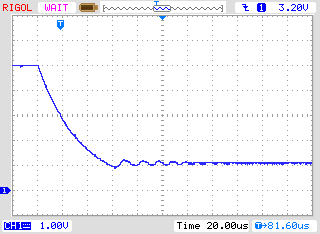
\includegraphics[width=.95\textwidth]{../PNG/AREF2_1V.png}
    \caption{from \(5V\) to \(1.1V\) }
    \label{pic:aref1}
  \end{subfigure}
  ~
  \begin{subfigure}[b]{.5\textwidth}
    \centering
    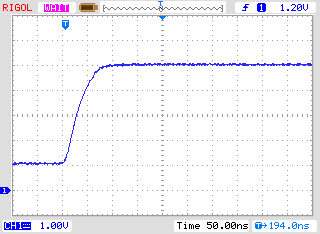
\includegraphics[width=.95\textwidth]{../PNG/AREF2VCC.png}
    \caption{from \(1.1V\) to \(5V\)}
    \label{pic:aref5}
  \end{subfigure}
  \caption{Umschalten von AREF mit einem \(1nF\) Kondensator}
\end{figure}

\begin{description} \setlength{\itemsep}{0em}
  \item[REF\_R\_KORR] gibt einen Offset für die interne Referenz-Spannung in mV-Einheiten an.
Mit diesem Offset kann eine Differenz bei der Umschaltung der Referenzspannung für die Widerstandsmessung abgeglichen werden.
Wenn die AUTO\_CAL-Option gewählt wurde, ist dieser Wert nur ein Offset zu der gefundenen Spannungs-Differenz in der
AUTO\_CAL Funktion.\\
Beispiel: CFLAGS += -DREF\_R\_KORR=10
  \item[OP\_MHZ] gibt der Software an, mit welcher Taktfrequenz in MHz der Tester arbeiten wird.
Die Software ist nur mit \(1MHz\), \(8MHz\) und zusätzlich auch \(16MHz\) getestet. Der Betrieb mit \(8MHz\) wird wegen der besseren Auflösung der
Kondensator- und Spulen-Messung empfohlen.\\
Beispiel: OP\_MHZ = 8
  \item[RESTART\_DELAY\_TICS] muss auf 6 gesetzt werden, wenn der ATmega168 oder ATmega328 ohne Quarz mit dem
RC-Generator betrieben wird. Wenn dieser Wert nicht vorbesetzt wird, wählt die Software die 16384 Takte Startverzögerung für
den Quarzbetrieb.\\
Beispiel: CFLAGS += -DRESTART\_DELAY\_TICS = 6
  \item[USE\_EEPROM] gibt an, ob feste Texte und Tabellen im EEPROM-Speicher abgelegt werden sollen.
Anderenfalls wird der Programmspeicher (Flash) benutzt.
Es wird empfohlen, den EEPROM-Speicher zu benutzen (Option gesetzt).\\
Beispiel: CFLAGS += -DUSE\_EEPROM
  \item[EBC\_STYLE] gibt an, dass die Ausgabe der Transistor-Pinbelegung im Format \inquotes{EBC=...} bzw. \inquotes{GDS=...} erfolgen soll.
  Diese Darstellungsweise spart Programmplatz. Ohne diese Option wird die Belegung im Format \inquotes{123=...} angezeigt, wobei
jeder Punkt ein E (Emitter), B (Basis) oder K (Kollektor) sein kann.
Bei FETs kann jeder Punkt entsprechend ein G (Gate), D (Drain) oder S (Source) sein.
Wenn die Reihenfolge der Testpins nicht 1,2 und 3 in Leserichtung ist, kann die Reihenfolge mit der Option EBC\_STYLE=321 
umgedreht werden. Dann wird die Pinbelegung in der Form \inquotes{321=...}, was der gewohnten Leserichtung von links nach rechts
entgegen kommt, wenn die Testpins die Reihenfolge 3,2,1 haben.\\
Beispiel: CFLAGS += EBC\_STYLE
  \item[NO\_NANO] gibt an, dass der Dezimalpräfix Nano nicht zur Darstellung von Messergebnissen benutzt werden soll.
So werden Kapazitätswerte in \(\mu F\) statt in \(nF\) angegeben.\\
Beispiel: CFLAGS += NO\_NANO
  \item[NO\_LONG\_PINLAYOUT] kann gesetzt werden, um die lange Form der Pinbelegung bei graphischen Displays zu verhindern
wie \inquotes{ Pin  1=E 2=B 3=C}.
Wenn die Option gesetzt ist, wird die kurze Form wie \inquotes{ Pin  123=EBC} benutzt.\\
Example: CFLAGS += NO\_LONG\_PINLAYOUT
  \item[PULLUP\_DISABLE] gibt an, dass man die internen \inquotes{Pull-Up}-Widerstände nicht benötigt.
Sie müssen einen externen \inquotes{Pull-Up} Widerstand an Pin 13 (PD7) und VCC angeschlossen haben, um diese
Option benutzen zu können.
Mit dieser Option wird ein möglicher Einfluss der \inquotes{Pull-Up} Widerstände auf die Mess-Ports (Port B und Port C) verhindert.\\
Beispiel: CFLAGS += -DPULLUP\_DISABLE

  \item[ANZ\_MESS] diese Option gibt an, wie oft der ADC-Wert eingelesen und addiert werden soll.
Sie können einen Wert zwischen 5 und 200 wählen um einen Mittelwert für eine ADC-Messung zu bilden.
Höhere Werte ergeben eine bessere Genauigkeit, aber brauchen längere Messzeit.
Eine ADC-Messung mit dem Wert 44 braucht etwa \(5ms\).\\
Beispiel: CFLAGS += -DANZ\_MESS=44

  \item[POWER\_OFF] Diese Option schaltet die automatische Abschaltfunktion ein.
Wenn Sie diese Option weglassen, werden die Messungen in einer Schleife endlos wiederholt, bis die Betriebsspannung 
unterbrochen wird (Ein/Aus-Schalter).
Wenn Sie einen Tester ohne die Schalttransistoren haben, können Sie diese Option weglassen.

Wenn Sie mit den eingebauten Schalttransistoren die Option POWER\_OFF weggelassen haben,
gibt es dennoch eine Möglichkeit für eine Abschaltung, wenn Sie die WITH\_MENU-Option gewählt haben.

Sie können mit der POWER\_OFF-Option auch angeben, nach wie vielen Messungen ohne gefundenes Bauteil der Tester ausschaltet.
Bei doppelt so viel aufeinanderfolgenden Messungen mit gefundenem Bauteil schaltet der Tester auch ab,
wenn nicht zwischendurch eine Messung ohne gefundenes Bauteil war.
Wenn Sie vergessen haben, ein angeschlossenes Bauteil abzuklemmen, wird so eine vollständige Batterie-Entladung
verhindert.
Bei einer Options-Angabe in der Form von CFLAGS += -DPOWER\_OFF=5 wird nach 5 aufeinanderfolgenden Messungen ohne
gefundenes Bauteil abschaltet. Aufeinanderfolgende 10 Messungen mit gefundenem Bauteil schalten ebenfalls aus.
Nur wenn die jeweilige Mess-Serie durch den anderen Typ unterbrochen wird, wird die Messung fortgesetzt.
Die Messresultate für eine Einzelmessung werden 28~Sekunden angezeigt, bei der Mehrfachmessung wird die
Anzeigezeit auf 5~Sekunden reduziert (wird in config.h gesetzt).
Wenn der Startknopf beim ersten Einschalten lange gedrückt wird, wird das Messergebnis
 auch bei der Mehrfachmessung 28~Sekunden angezeigt.
Der Maximalwert für die Wiederholungen ist 255 (CFLAGS += -DPOWER\_OFF=255).\\
Beispiel 1: CFLAGS += -DPOWER\_OFF=5 \\
Beispiel 2: CFLAGS += -DPOWER\_OFF 

  \item[BAT\_CHECK] schaltet die Batterie-Spannungsprüfung ein.
 Wenn Sie diese Option nicht angeben, wird die Versionsnummer der Software angezeigt.
Diese Option ist hilfreich um bei batteriebetriebenen Tester-Versionen an den Batteriewechsel zu erinnern.\\
Beispiel: CFLAGS += -DBAT\_CHECK

  \item[BAT\_OUT] schaltet die Batterie-Spannungsanzeige auf dem LCD ein, wenn BAT\_CHECK gewählt wurde.
 Wenn Ihre \(9V\)-Versorgung eine Diode als Verpolungsschutz installiert hat, können Sie 
die Form BAT\_OUT=600 angeben, um die Dioden-Schwellspannung 
bei der Spannungsanzeige zu berücksichtigen.
Auch der Spannungsverlust am Transistor T3 kann so mit dieser Option berücksichtigt werden.
Die Angabe der Schwellspannung in mV beeinflusst nicht die Prüf\-span\-nungs Werte (BAT\_POOR).\\
Beispiel 1: CFLAGS += -DBAT\_OUT=300 \\
Beispiel 2: CFLAGS += -DBAT\_OUT

  \item[BAT\_POOR] setzt die Leer-Spannung für die Batteriespannungs-Prüfung auf den angegebenen Wert in Einheiten von \(1mV\).
Die Warn-Spannung ist \(0,8V\) höher als die angegebene Leer-Spannung, wenn die Leer-Spannung mehr als \(5,3V\) beträgt.
Sonst wird eine \(0,4V\) höhere Warn-Spannung gewählt, bei unter \(3,25V\) sogar nur eine \(0,2V\) höhere Warn-Spannung und
bei unter \(1,3V\) nur eine \(0,1V\) höhere Warnspannung als die angegebene Leer-Spannung.
Das Setzen der Leer-Spannung auf Werte wie \(5,4V\) wird für wiederaufladbare \(9V\) Batterien nicht empfohlen,
weil das die Gefahr von Batterie-Schäden aufgrund von Tiefentladung erhöht!
Wenn Sie wiederaufladbare \(9V\)-Batterien einsetzen, werden \inquotes{Ready to Use}-Typen wegen der geringeren Selbstentladung empfohlen.\\
Beispiel für low-drop-Regler (\(5,4V\)): CFLAGS += -DBAT\_POOR=5400 \\
Beispiel für 7805-Regler (\(6,4V\)): CFLAGS += -DBAT\_POOR=6400

  \item[DC\_PWR] Dieser Spannungspegel in mV Einheiten gibt eine Grenze für die Batteriespannung an, oberhalb
  derer der Tester in den \inquotes{DC\_Pwr\_Mode} wechselt. Normalerweise läuft der Tester in einem Batterie-Modus,
wo alle Zusatzfunktionen zeitlich beschränkt laufen.
Mit dem \inquotes{DC\_Pwr\_Mode} laufen die Zusatzfunktionen zeitlich unbeschränkt.
Weil es keinen DC-DC Konverter gibt, der mit einer Eingangsspannung von \(0.9V\) läuft,
wird der \inquotes{DC\_Pwr\_Mode} auch gestartet, wenn eine Batteriespannung unterhalb \(0.9V\) entdeckt wird.\\
Beispiel: CFLAGS += -DDC\_PWR=9500

 \item[BAT\_NUMERATOR] Definiert den Zähler eines Bruchs an, mit dem die Spannung bewertet werden muß,
um die richtige Batteriespannung zu erhalten. Für den Standard-Spannungsteiler mit einem \(10 k\Omega\) und 
einem \(3.3 k\Omega\) Widerstand ist der Quotient (10000 + 3300)/3300. 
Der über die Widerstandswerte erhaltene Quotient sollte gekürzt werden. 
Für das Beispiel ergibt sich 133/33 .\\
Beispiel: CFLAGS += -DBAT\_NUMERATOR=133

 \item[BAT\_DENOMINATOR] Gibt den Nenner eines Bruches an, mit dem die Spannung bewertet werden muß.\\
Beispiel: CFLAGS += -DBAT\_DENOMINATOR=33

 \item[EXT\_NUMERATOR] Definiert den Zähler eines Bruchs an, mit dem die externe Spannung bewertet werden muß,
um die richtige Spannung zu erhalten. Für den Standard-Spannungsteiler mit einem \(180 k\Omega\) und 
einem \(20 k\Omega\) Widerstand ist der Quotient (180000+20000)/20000.
Der Quotient sollte auf 10/1 gekürzt werden.\\
Beispiel: CFLAGS += -DEXT\_NUMERATOR=10

 \item[EXT\_DENOMINATOR] Gibt den Nenner eines Bruches an, mit dem die externe Spannung bewertet werden muß.\\
Beispiel: CFLAGS += -DEXT\_DENOMINATOR=1

  \item[INHIBIT\_SLEEP\_MODE] sperrt die Benutzung des \inquotes{Sleep Mode} (Schlafzustand) des Prozessors.
Normalerweise wird von der Software für längere Pausen der Schlafzustand des Prozessors benutzt, um Strom zu sparen.
Die Benutzung dieses Schlafzustandes mit dem Wiederaufwachen spart zwar Batteriekapazität, 
stellt eine zusätzliche Anforderung für den Spannungsregler dar.\\
Beispiel: DINHIBIT\_SLEEP\_MODE = 1

  \item[PROGRAMMER] \label{sec:config-Prog} stellt den Programmer-Typ für das \lcmd{avrdude} Schnittstellenprogramm ein.\\
Eine richtige Einstellung des Programmer-Typs (und Ports) ist notwendig.\\
In \lname{Makefile} ist standardmäßig Programmer der Firma Diamex eingestellt.\\
Vorbereitet sind aber auch USBasp von Fischler und Arduino Mega.\\
Falls ein anderer Programmer verwendet sein sollte, muss er in \lname{Makefile} aufgenommen werden und der,
bis jetzt aktuelle, mit \#~ am Anfang der Zeile abgewählt werden.\\
Ein Beispiel für die Benutzung von USBtiny Programmer:\\
\# setting for USBtiny ISP\\
PROGRAMMER=usbtiny\\
BitClock=10\\
PORT=usb\\
und ein weiterer Beispiel:\\
\#~setting for Pololu programmer\\
\#~PROGRAMMER=stk500v2\\
\#~BitClock=1.0\\
\#~PORT = /dev/ttyACM0\\
, wenn Sie den \lcmd{make upload}- oder
\lcmd{make fuses}-Aufruf dieser \lname{Makefile} benutzen.
Beispiel: PROGRAMMER=avrisp2

  \item[BitClock] stellt die Bit-Taktperiode für den Programmer ein. Siehe dazu die Beschreibung des -B Parameters von \lcmd{avrdude}.\\
Beispiel: BitClock=5.0

  \item[PORT] stellt die verwendete Schnittstelle ein, wo \lcmd{avrdude} den Mikrocontroller (ATmega) erreichen kann.
  Für weitere Informationen schauen Sie bitte in das Handbuch von \lcmd{avrdude} oder in die Online-Dokumentation~\cite{avrdude}.\\
Beispiel: PORT=usb

\end{description}

Zusätzliche Parameter können in den Dateien Transistortester.h und config.h gesetzt werden.
Die Datei config.h enthält globale Variablen und Tabellen, definiert die Port- / Pin-Konstellation,
die ADC-Taktfrequenz sowie die Widerstandswerte, die für die Messung benutzt werden.
Die Datei Transistortester.h enthält die globalen Variablen und Tabellen sowie die Texte für die LCD-Anzeige.
Normalerweise brauchen diese Werte nicht ohne Grund geändert werden.


\section{Programmierung des Mikrocontrollers}
Ich gebe die Software für den Mikrocontroller in Quelltext heraus.
Die Entwicklung wurde mit dem Linux-Betriebssystem (Ubuntu bzw. Mint) gemacht
und wird gesteuert mit einer \lname{Makefile}.

Die \lname{Makefile} stellt sicher, dass die Software entsprechend der vorher in der \lname{Makefile} 
eingestellten Optionen übersetzt wird. Schauen Sie bitte in die Datei LiesMich.txt
im Verzeichnis default und in das Konfigurations-Kapitel~\ref{sec:config} ab Seite~\pageref{sec:config}.

Das Ergebnis der Übersetzung hat die Dateierweiterung \lname{.hex} und \lname{.eep}.
Die \lname{.hex}-Datei enthält die Daten für den Programmspeicher (Flash) des ATmega-Prozessors.
Die \lname{.eep}-Datei enthält die Daten für den EEPROM des ATmega.\\
Beide Dateien müssen in den richtigen Speicher geladen werden.

Zusätzlich muss der ATmega mit den \inquotes{fuses} richtig konfiguriert werden.\\
Wenn Sie meine \lname{Makefile} zusammen mit dem Programm \lcmd{avrdude} \cite{avrdude} benutzen,
brauchen Sie keine genaue Kenntnis über die Einzelheiten der fuses.

Sie brauchen nur \lcmd{make fuses} aufrufen, wenn Sie keinen Quarz benutzen oder Sie
müssen \lcmd{make fuses-crystal} aufrufen, wenn Sie einen \(8MHz\) Quarz auf der Baugruppe installiert haben.

Bei der ATmega168-Serie der Mikrocontroller können Sie alternativ auch
\lcmd{make fuses-crystal-lp} aufrufen für den low power Quarz-Betrieb.\\
Benutzen Sie niemals die Quarz-Varianten, wenn Sie keinen \(8MHz\) oder \(16MHz\) Quarz installiert haben.

Wenn Sie sich nicht sicher mit den fuses sind, lassen Sie diese erst einmal wie
vom Werk gesetzt und bringen Sie den Tester in diesem Zustand zum Laufen.\\
Es kann sein, dass das Programm zu langsam läuft, wenn Sie die für den \(8MHz\)-Betrieb 
erzeugten Programmdaten benutzen, aber das kann man später korrigieren!
Aber falsch gesetzte fuses können die spätere ISP-Programmierung verhindern.

Vielleicht meldet das Programm \lcmd{avrdude} einen Fehler beim Setzen der extendet Fuse efuse.
Das Lesen von unbenutzten Fuse Bits ist beim ATmega als \inquotes{1} spezifiziert, aber
das \lcmd{avrdude} Programm maskiert die unbenutzten Bits, so daß es eine \inquotes{0} für alle unbenutzen Bits erwartet.
Normalerweise sollte die efuse auf 0xfc gesetzt werden, aber \lcmd{avrdude} liest eine 0x04 mit der Maske zurück.
Man kann die Datei avrdude.conf ändern, um das Verhalten von \lcmd{avrdude} zu ändern oder
die efuse auf 0x04 setzen. 
Alle efuse-Werte können mit dem Bezeichner EFUSE\_VAL am Anfang der Datei setup.mk im Quellcode-Verzeichnis
gesetzt werden. Wahrscheinlich sind die Fuses aber auch mit der Fehlermeldung richtig gesetzt.

\newpage
\subsection{Benutzung von Linux}
\label{sec:linux}

Um meine Erfahrung mit Verzweiflung und \inquotes{schlaflose Nächten} anderen Kollegen zu ersparen,
wurde dieses Unterkapitel geschrieben.
Ich hatte ohne jegliche AVR Erfahrung einen Clonetester erworben und wollte diesem die deutsche Sprache
\inquotes{beibringen}.\\

Die dabei erworbenen Erfahrungen sollen anderen \inquotes{willigen} Unerfahrenen helfen,
ERFOLGREICH ihren Tester zu programmieren.
Diese Gelegenheit wird benutzt, dem Entwickler des Transistortester und Autor dieses Dokuments,  
Karl-Heinz Kübbeler siehe \cite{karlheinz1} zu danken für sein Engagement und Geduld,
denn die folgenden Seiten wären ohne seine Hilfe nie entstanden.
     
Damit das Übersetzen der Firmware und Brennen ins MCU gelingt und gleichzeitig \dots
\inquotes{das Rad nicht neu erfunden werden muss}, wurde ein Teil der folgenden Seiten aus dem
ursprünglichen Original übernommen.

Also noch einmal \dots \LARGE{EINEN RIESEN DANK}
\normalsize an Karl-Heinz Kübbeler.

\subsubsection{Betriebssystem Linux}

Die Programmierung unten Linux bringt viele Vorteile, weil dieses OS von Experten entwickelt wurde,
die sich auf den Wünschen der Benutzer orientieren.
Zudem ist die Umgebung kostenlos erhältlich und perfekt gewartet.
Ein weiterer Vorteil ist die Sicherheit des OS selbst aber auch beim Nutzen des Internets.
Die heutigen Editionen lassen sich noch viel leichter bedienen als die Mitbewerber OS.
Es gibt auch sehr leistungsfähige Editoren wie vim oder emacs, die aber etwas
Einarbeitungszeit erfordern. Speziell vim hat den Vorteil, daß er praktisch auf
jedem System vorinstalliert ist. Aber gerade bei diesem Editor ist der
Wechsel zwischen Eingabe-Modus und Befehls-Modus gewöhnungsbedürfig.
Diese Anleitung soll alle \inquotes{nicht} Linux Benutzer dazu animieren es NUN zu testen
indem sie ihr Tester damit programmieren.

Die nachfolgenden Beispiele wurden mit Linux Mint getestet, das
mit drei verschiedenen Desktop Umgebungen angeboten wird (cinnemon, MATE und Xfce).
Die nachfolgenden Hinweise sollten aber bei allen drei Desktops funktionieren.
Die Installation ist auf verschiedene Arten möglich und bringt seinen eigenen Bootmanager mit,
damit man sein vorhandenes OS weiter parallel nutzen kann.

\subsubsection{Tipps für die Linux Nutzung}

Zuerst möchte ich einen Hinweis geben für alle, die nicht gerne Texte abschreiben.
Sie können dieses Handbuch auf einen USB-Stick kopieren und im Dateibrowser mit Doppelclick der
linken Maustaste \LMB öffnen.
Alternativ zum Doppelklick kann mit der \RMB Taste ein anderes als das
vorgewählte PDF Betrachtungsprogramm ausgewählt werden.
Das geöffnete Fenster kann auf dem Bildschirm verschoben werden und auch in der Größe
angepasst werden. Dazu gibt es in der Regel verschiedene Möglichkeiten.
Eine davon ist die \RMB Taste zu drücken, wenn der Mauszeiger 
auf die Kopfzeile des Fensters zeigt und dann die Funktion \menu[,]{Verschieben} auszuwählen.
So kann man das Fenster mit der PDF-Dokumentation beispielsweise an die linke Bildschirmseite
verschieben. Durch Drücken der linken Maustaste rastet das Fenster an der neuen Position ein.
Zum Verschieben kann man auch mit der \LMB Taste die
Kopfleiste des Fensters packen und bei weiter gedrückter \LMB Taste verschieben.
Dann rastet das Fenster auf der Position ein, wenn man die Maustaste loslässt.

Im nächsten Schritt wird die Tastenkombination \keys{{Strg} + \Alt + T} gleichzeitig gedrückt,
um ein (neues) Befehlsfenster zu öffnen.
Dies wird nun auf die schon beschriebene Weise zur rechten Hälfte des Bildschirmes verschoben und
kann auch in der Größe verändert werden.
Die Größenänderung kann mit der \LMB Taste an den Rändern oder Ecken des Fenstern gemacht werden,
oder auch mit der \RMB Taste an der Kopfleiste mit der \menu[,]{{Größe ändern}} Funktion.
Die Bedienung ist sonst gleich wie beim Verschieben.\\

In der Regel besitzen die graphischen Oberflächen bei Linux mehr als eine Arbeitsfläche,
die mit der Tastenkombination \keys{{Strg} + \Alt + \arrowkeyright}
beziehungsweise \keys{{Strg} + \Alt + \arrowkeyleft} umgeschaltet werden können.
Mit der \RMB Taste können Sie auf der Kopfzeile der Fenster eine
der Arbeitsflächen wählen, auf der das Fenster angezeigt wird.

So kann man die für die Arbeit benötigten Fenster auf einer Arbeitfläche
zusammen sammeln und erstickt nicht in all den Fenstern für verschiedene Arbeitsbereiche. 
Bei allen Befehlseingaben und Dateibezeichnern ist übrigens darauf zu  achten,
daß bei Linux zwischen Groß und Kleinschreibung unterschieden wird.


\subsubsection{Programm Pakete installieren}

Zum Installieren von Software-Paketen braucht ihr Rechner einen Internetzugang.
Bevor Sie den Tester programmieren konnen, müssen zuerst die Programmpakete
binutils-avr, avrdude, avr-libc und gcc-avr installiert werden.
Jetzt können sie den unten angegebenen Befehl durch Abtippen
mit der Tastatur ausführen lassen.
Sie können aber auch im geöffneten PDF Dokument an diese Stelle blättern
und den nachfolgenden Text mit der gedückten linken Maustaste \LMB markieren:
\begin{large} \vspace{-0.4em} \begin{verbatim}
sudo apt-get install avrdude avr-libc binutils-avr gcc-avr git
\end{verbatim} \end{large}
Am Ende des Textes muß die Maustaste \LMB losgelassen werden,
um die Markierung abzuschließen.
wenn der Text in einer eigenen Zeile steht, wie in diesem Beispiel, können
die den Text auch mit dreimaligem \LMB Maus Click irgendwo auf der Zeile markieren.
Danach kann man den Mauszeiger in das rechte Befehlsfenster führen und
durch Drücken der mittlerer Maustaste {weiter als \MMB abgekürzt} den vorhin
markierten Text in die Befehlszeile einfügen.
Bei vielen Mäusen ist das Scoll-Rad gleichzeitig die mittlere Maustaste.
Bei Mäusen ohne mittlere Maustaste ist es möglich die mittlere Maustaste
durch gleichzeitiges Drücken der \LRMB Maustasten zu ersetzen.
Egal, wie der Befehlstext nun in die Befehlszeile gekommen ist,
sie sollten den Text noch einmal kontrollieren, bevor
sie den Befehl durch Dücken der \keys{\enter} Taste abschicken.
In der Regel brauchen Sie keine Angst zu haben, daß durch die Installation
von Paketen etwas schlimmes durch Fehlbedienung passiert.
Das Programm \lcmd{apt-get} prüft vor dem Ausführen der Operation, ob die aufgeführten
Pakete schon installiert sind und die Abhängigkeiten erfüllt sind.
Gegebenenfalls wird aber ein schon vorher installiertes Paket durch ein neueres ersetzt.
Dann wird das \lcmd{sudo} Programm Sie zunächst nach den Benutzer Passwort fragen,
bevor es den Rest der Befehlszeile ausführt.
Sie sollten das Passwort mit Drücken der \keys{\enter} oder \keys{\return} Taste abschließen und bestätigen.
Damit werden nun alle Software Pakete durch \lcmd{apt-get} herunter geladen und installiert.\\

Es kann sein, daß \lcmd{apt-get} bei der Installation der Pakete Fragen stellt,
die man in der Regel mit der Taste \keys{J} beantworten kann.

Natürlich gibt es auch andere Wege, die Pakete zu installieren, welche eine graphische Oberfläche benutzen
wie \lcmd{synaptic} oder \lcmd{dpkg}. Aber es nicht einfacher eine gemischte Gruppe von Paketen anzugeben.
Wenn sie irgendeine dieser Paketmanager, sollten sie über alle installierten Pakete Bescheid wissen,
egal auf welchem Wege sie installiert wurden.
Die graphischen Paketmanager können auch dabei helfen, den Namen der Pakete herauszufinden.

\subsubsection{Download der Quellen}

Ob die Versionsverwaltung \lcmd{git} erfolgreich installiert wurde,
kann man mit dem folgenden Kommando prüfen:
\begin{large} \vspace{-0.4em} \begin{verbatim}
git version
\end{verbatim} \end{large}
Das \lcmd{git} Programm sollte mit der Ausgabe seiner Versionsnummer antworten.
Falls in Ihrem Heimatverzeichnis schon ein Ordner TransistorTester-source existiert,
sollte man den umbenennen oder löschen.
Das Programm \lcmd{git} wird für den Download der Quellen und Dokumentation benutzt.
Mit dem Befehl:
\begin{large} \vspace{-0.4em} \begin{verbatim}
git clone https://github.com/kubi48/TransistorTester-source
\end{verbatim} \end{large}
wird das aktuelle Transistortester Quellcode-Archiv heruntergeladen.
Die Dateien sind nun in dem Linux [Persönlicher Ordner] , üblicherweise \lname{/home/} gefolgt
von Ihrem Benutzerkürzel, mit dem  Verzeichnisnamen \lname{TransistorTester-source}.
Mit der Terminaleingabe  \lcmd{ls} \(\mbox{\keys{l} \keys{s} \keys{\return}}\) kann man
das Vorhandensein überprüfen.
Mehr Informationen über Dateien und Verzeichnisse erhält man mit
dem Kommando \lcmd{ls -lh}. Hier wurden jetzt zwei Optionen für das Kommando \lcmd{ls} zusammengefasst,
die \lcmd{{ -l}} Option und die \lcmd{{ -h}} Option. Diese Eingabeform ist also eine Kurzform für
das Kommando \lcmd{ls -l -h} oder auch \lcmd{ls -l {-}{-}human-readable}.
Einige der Optionen sind in zwei Versionen vorhanden, einer kurzen mit einem - (\lcmd{{ -h}})
und einer langen Form mit zwei - (\lcmd{{ {-}{-}human-readable}}).
Die Reihenfolge der Optionen spielt übrigens keine Rolle,
genau wie die Anzahl der trennenden Leerzeichen \keys{\space}.
Bei fast allen Kommandos erfährt man mehr über die Bedienung und die Optionen
durch durch Anhängen der \lcmd{{ --help}} Option.
Das gilt natürlich auch für das Kommando \lcmd{git}.\\

Um neue Updates heruntergeladen, reicht es in der Zukunft, 
\begin{large} \vspace{-0.4em} \begin{verbatim}
git pull
\end{verbatim} \end{large}
im Arbeitsverzeichnis \lname{TransistorTester-source} einzugeben.
Das kann je nach Kommandointerpreter auch mit
\begin{large} \vspace{-0.4em} \begin{verbatim}
(cd ~/TransistorTester-source ; git pull)
\end{verbatim} \end{large}
aus jedem Arbeisverzeichnis erfolgen.
Damit der \lcmd{git pull} einwandfrei funktioniert, sollte man den
Verzeichnisbaum besser nicht verändern.

\subsubsection{Übersetzen der Transistortester Quellen}

Zum Übersetzen der Transistortester-Quellen ist nur ein \lcmd{make} Aufruf
im richtigen Arbeitsverzeichnis erforderlich.
Da aber auch mit \lcmd{make upload} der ATmega mit einem angeschlossenen
ISP-Programmer programmiert werden kann, ist es sinnvoll,
sich zunächst mit den Schnittstellen für den Anschluß des ISP-Programmer
zu beschäftigen.
Der weitere Arbeitsablauf ist dann unter Punkt \ref{sec:Arbeitsumgebung} auf
Seite \pageref{sec:Arbeitsumgebung} beschrieben.

\subsubsection{Benutzung der Schnittstellen}
\label{sec:Schnittstellen}

Alle modernen ISP-Programmer mit serieller Schnittstelle benutzen gerne die USB Schnittstelle,
da diese Schnittstelle auch gleich die Stromversorgung sicherstellt.
Für diese Geräte sollten Sie überprüfen, welche Gerätebezeichnung
diesem Gerät zugeordnet ist.
Beim Einstecken eines USB Gerätes wird bei Linux ein Eintrag in das
Systemprotokoll vorgenommen.
Da das Systemprotokoll eine Textdatei ist,
kann man diese einfach auf dem Bildschirm anzeigen.
Dazu kann man in Konsolfenster den Befehl dmesg benutzen und da wir nach dem
Einstecken des Programmers nur an den letzten Zeilen des Protokolls
interessiert sind, benutzt man:
\begin{large} \vspace{-0.4em} \begin{verbatim}
dmesg|tail
\end{verbatim} \end{large}
Das \lcmd{dmesg} Programm zeigt das gesamte Systemprotokoll und das Kommando 
\lcmd{tail} zeigt nur die letzten 10 Zeilen der Ausgabe.
Für einen Pololu Programmer sieht das Ergebnis so aus:
\begin{footnotesize} \begin{verbatim}
usb 1-3: new full-speed USB device number 3 using xhci_hcd
usb 1-3: New USB device found, idVendor=1ffb, idProduct=00bb, bcdDevice= 1.02
usb 1-3: New USB device strings: Mfr=1, Product=2, SerialNumber=3
usb 1-3: Product: Pololu USB AVR Programmer v2.1
usb 1-3: Manufacturer: Pololu Corporation
usb 1-3: SerialNumber: 00227484
cdc_acm 1-3:1.1: ttyACM0: USB ACM device
cdc_acm 1-3:1.3: ttyACM1: USB ACM device
usbcore: registered new interface driver cdc_acm
cdc_acm: USB Abstract Control Model driver for USB modems and ISDN adapters
\end{verbatim} \end{footnotesize}
Wichtig sind hier die Zeilen 7 und 8 mit den Einträgen ttyACM0 und ttyACM1.
Das sind die zugewiesenen Gerätebezeichnungen für zwei serielle Schnittstellen.
Bei Linux sind alle Geräte auch Bestandteil des Dateibaums und im
Ordner \lname{/dev/} eingetragen. Mit vollständigem Namen heißen die
beiden seriellen Schnittstellen also \lname{/dev/ttyACM0} und \lname{/dev/ttyACM1}.
Für den Pololu Programmer muß man wissen, daß die erste serielle Schnittstelle
für den ISP-Programmer benutzt wird und die zweite serielle Schnittstelle
für andere Zwecke frei benutzt werden kann.
Sie können die Existenz der Geräteeintragungen mit dem Kommando
\begin{large} \vspace{-0.4em} \begin{verbatim}
ls -l /dev/ttyACM*
\end{verbatim} \end{large}
überprüfen. Das Ergebnis sollte dann so aussehen:
\begin{footnotesize} \begin{verbatim}
crw-rw---- 1 root dialout 166, 0 Mär 11 09:57 /dev/ttyACM0
crw-rw---- 1 root dialout 166, 1 Mär 11 09:57 /dev/ttyACM1
\end{verbatim} \end{footnotesize}
Bei dieser Ausgabe kann man lesen, daß der Zugriff für den Benutzer \lname{root}
und für die Benutzergruppe \lname{dialout} erlaubt ist.
Mit dem Kommando \lcmd{id} können Sie ihre Gruppenzugehörigkeit überprüfen.
Hier sollte die Gruppe \lname{dialout} in der Liste auftauchen,
sonst wird im nächsten Arbeitspunkt die Änderung der Gruppenzugehörigkeit
beschrieben.
Ein anderes Beispiel für das Systemprotokoll eines anderen
ISP-Programmers \inquotes{Diamex ISP-PRog NG} sehen sie hier:
\begin{footnotesize} \begin{verbatim}
usb 1-6: new full-speed USB device number 8 using xhci_hcd
usb 1-6: New USB device found, idVendor=16c0, idProduct=2a9b, bcdDevice=43.40
usb 1-6: New USB device strings: Mfr=1, Product=2, SerialNumber=3
usb 1-6: Product: AVR-ISP2
usb 1-6: Manufacturer: ERFOS
usb 1-6: SerialNumber: 19377-43111-757
cdc_acm 1-6:1.0: ttyACM0: USB ACM device
\end{verbatim} \end{footnotesize}

Bei diesem Beispiel ist der Gerätename identisch (ttyACM0).\\

Einen Überblick über die angeschlossenen USB-seriell Wandler geben auch
die Eintragungen in Verzeichnis \lname{/dev/serial/by-id/},
die man mit dem Kommando abfragen kann:
\begin{large} \vspace{-0.4em} \begin{verbatim}
ls -og /dev/serial/by-id/* | cut -d' ' -f 7-
\end{verbatim} \end{large}
Die Ausgabe kann beispielsweise so aussehen:
\begin{footnotesize} \begin{verbatim}
/dev/serial/by-id/usb-Arduino__www.arduino.cc__0043_954323131383519062F0-if00 -> ../../ttyACM2
/dev/serial/by-id/usb-Pololu_Corporation_Pololu_USB_AVR_Programmer_v2.1_00227484-if01 -> ../../ttyACM0
/dev/serial/by-id/usb-Pololu_Corporation_Pololu_USB_AVR_Programmer_v2.1_00227484-if03 -> ../../ttyACM1
\end{verbatim} \end{footnotesize}
Wenn die Beschreibung ausführlich genug ist, kann man so die Schnittstellen zuordnen.


Wenn bis zu diesem Schritt alles in Ordnung ist,
muß für dieses Beispiel nur der PORT Eintrag in der \lname{Makefile} auf
\inquotes{PORT=/dev/ttyACM0} geändert werden,
damit das \lcmd{avrdude} Programm auf den Programmer zugreifen kann.
Wenn bei Ihrem System noch andere USB-seriell Schnittstellen benutzt
werden, können die letzten Ziffern der Gerätebezeichnung abweichen.
Erwähnen möchte ich auch, daß eine andere Gruppe von USB-seriell
Schnittstellen statt ttyACM den Namen ttyUSB verwendet.\\

Wenn Ihr Programmer eine spezielle USB-Schnittstelle benutzt und
keinen USB-seriell Typ, ist wahrscheinlich noch zusätzliche
Arbeit erforderlich. Als PORT kann hier fest \inquotes{usb} in der \lname{Makefile}
eingetragen werden. Es ist aber wahrscheinlich, daß Sie trotzdem
keinen Zugriff auf das Gerät haben.
Alle angeschlossenen USB-Geräte können durch Eingabe von \lcmd{lsusb} im Befehlsfenster 
angezeigt werden.
Geben Sie \lcmd{lsusb} zuerst ohne und dann mit angeschlossenem USB-Programmer ein.
Ein Vergleich der Ergebnisse lokalisiert den USB-Programmer.

Das Ergebnis von \lcmd{lsusb} kann so aussehen:
\begin{footnotesize} \begin{verbatim}
Bus 001 Device 001: ID 1d6b:0002 Linux Foundation 2.0 root hub
Bus 002 Device 003: ID 046d:c050 Logitech, Inc. RX 250 Optical Mouse
Bus 002 Device 058: ID 03eb:2104 Atmel Corp. AVR ISP mkII
Bus 002 Device 059: ID 2341:0042 Arduino SA Mega 2560 R3 (CDC ACM)
Bus 002 Device 001: ID 1d6b:0001 Linux Foundation 1.1 root hub}
\end{verbatim} \end{footnotesize}
Hier wurde als Device 58 ein AVR ISP mkII erkannt (DIAMEX ALL-AVR).
Das ebenfalls entdeckte Gerät mit der Nummer 59 gehört zur Gruppe der \inquotes{USB-seriell} Geräte.
Die ID 03eb ist eine Herstellerkennung und die ID 2104 eine Produktkennung für diesen ISP-Programmer.
Diese beiden Kennungen werden der Datei /etc/udev/rules.d/90-atmel.rules benötigt und erstellt
mit Hilfe von:
\begin{large} \vspace{-0.4em} \begin{verbatim}
sudo xed /etc/udev/rules.d/90-atmel.rules
\end{verbatim} \end{large}
Natürlich können Sie auch einen anderen Editor als xed benutzen, wenn Sie möchten.
In diesem Beispiel besteht die Datei 90-atmel.rules aus einer Zeile:
\begin{footnotesize} \vspace{-0.4em} \begin{verbatim}
SUBSYSTEM=="usb", ATTRS{idVendor}=="03eb", ATTRS{idProduct}=="2104", MODE="0660", GROUP="plugdev"
\end{verbatim} \end{footnotesize}
Dieser Eintrag erlaubt den Zugriff auf das Gerät für Mitglieder der Gruppe \lname{plugdev}.
Man kann den Eintrag auch ohne Editor direkt mit einem Kommando erzeugen:
\begin{footnotesize} \vspace{-0.4em} \begin{verbatim}
sudo echo 'SUBSYSTEM=="usb", ATTRS{idVendor}=="03eb", ATTRS{idProduct}=="2104"
, MODE="0660", GROUP="plugdev"' >> /etc/udev/rules.d/90-atmel.rules
\end{verbatim} \end{footnotesize}
Die beiden Zeilen müssen sie zu einer langen Zeile 
in der Kommandozeile zusammenfügen!
\newline
Um die meisten Programmer verwenden zu können, wird folgender Text in 90-atmel.rules empfohlen:
\begin{tiny}
\begin{verbatim}
# Copy this file to /etc/udev/rules.d/90-atmel.rules
# AVR ISP mkII - DIAMEX ALL-AVR
SUBSYSTEM=="usb", ATTRS {idVendor}=="03eb", ATTRS {idProduct}=="2104", GROUP = "plugdev", MODE="0660",
# Atmel AVR Dragon
ATTRS {idVendor}=="03eb", ATTRS {idProduct}=="2107", GROUP="plugdev", MODE="0660"
# Atmel-ICE
SUBSYSTEM=="usb", ATTRS {idVendor}=="03eb", ATTRS {idProduct}=="2141", GROUP = "plugdev", MODE="0660",
# xplained-mini
SUBSYSTEM=="usb", ATTRS {idVendor}=="03eb", ATTRS {idProduct}=="2145", GROUP = "plugdev", MODE="0660",
# avrftdi
#SUBSYSTEM=="usb", ATTRS {idVendor}=="0403, ATTRS {idProduct}=="6010", GROUP = "plugdev", MODE="0660",
# UM232H
#SUBSYSTEM=="usb", ATTRS {idVendor}=="0403, ATTRS {idProduct}=="6014", GROUP = "plugdev", MODE="0660",
# USB asp programmer
ATTRS {idVendor}=="16c0", ATTRS {idProduct}=="05dc", GROUP="plugdev", MODE="0660"
# USB NIBObee-Programmer
ATTRS {idVendor}=="16c0", ATTRS {idProduct}=="092f", GROUP="plugdev", MODE="0660"
# USBtiny programmer
ATTRS {idVendor}=="1781", ATTRS {idProduct}=="0c9f", GROUP="plugdev", MODE="0660"
# USB ISP-programmer für Atmel AVR
SUBSYSTEM=="usb", ENV {DEVTYPE}=="usb_device", SYSFS {idVendor}=="16c0", SYSFS {idProduct} == "05dc", MODE="0660",
\end{verbatim}
\end{tiny}
\vspace*{-.8em}
Nach dem die Datei erstellt wurde, kann die Erstellung und Inhalt kontrollieren mit:
\begin{large} \vspace{-0.4em} \begin{verbatim}
less /etc/udev/rules.d/90-atmel.rules 
\end{verbatim} \end{large}
Danach sollten Sie das System veranlassen, die udev-Regeln neu einzulesen mit:
\begin{large} \vspace{-0.4em} \begin{verbatim}
sudo udevadm control --reload-rules
\end{verbatim} \end{large}
Dann sollten Sie den ISP-Programmer ausstecken und wieder einstecken.
Jetzt sollte das System Ihnen Zugriff auf das Gerät geben, wenn Sie Mitglied der Gruppe \lname{plugdev}
sind.
Daher sollten Sie Mitglied der Gruppe \lname{plugdev} und auch der Gruppe \lname{dialout}
sein, damit Sie beide ISP-Programmertypen nutzen können.

\subsubsection{Gruppen Mitgliedschaft}

Deswegen sollte die eigene Benutzerkennung sowohl Mitglied der Gruppe \lname{plugdev} als auch
der Gruppe \lname{dialout} sein. Das Kommando:
\begin{large} \vspace{-0.4em} \begin{verbatim}
sudo usermod -a -G dialout,plugdev $USER
\end{verbatim} \end{large}
sollte die Zugehörigkeit sicherstellen. 
Kontrollieren kann man es mit dem Kommando: \lcmd{id}. 
Wenn die Gruppenmitgliedschaft richtig gemeldet wird,
sollte jetzt ein Zugriff mit \lcmd{avrdude} auf ISP-Programmer mit beiden Schnittstellentypen möglich sein.

Mann kann sich die Gruppenmitgliedschaft auch mit einem Programm mit graphischer Bedienoberfläche ansehen:
\menu[,]{Menü,Systemverwaltung,{Benutzer und Gruppen},{?Passwort}}.
Das \menu[,]{Menü} kann man auch mit der \keys{\winmenu} Taste (zwischen \keys{{Strg}} und
\keys{\Alt}) öffnen.
Aber das Layout der Funktion ist unterschiedlich je nach Desktop Umgebung.

\subsubsection{Arbeitsumgebung und Übersetzen der Quellen}
\label{sec:Arbeitsumgebung}
Damit das Original erhalten bleibt,
wird empfohlen, ein Duplikat der Quellen mit Namen \textbf {Mytester} anzulegen.
Üblicherweise heißt das Home-Verzeichnis \lname{/home/} gefolgt von ihrem Benutzerkürzel.
Der Name ihres Home-Verzeichnisses ist in der System-Variablen \lname{\$HOME} abgelegt.
Sie können statt des Namens in Befehlen auch kurz \lname{\textasciitilde/} schreiben.
Vergessen sie nicht den \lname{/} nach dem \lname{\textasciitilde} Zeichen, sonst würde der
Kommandointerpreter nach einem Benutzer mit dem nachfolgenden Namen suchen!
Dazu legen Sie erst einmal ein leeres Verzeichnis an mit:
\begin{large} \vspace{-0.4em} \begin{verbatim}
mkdir ~/Mytester
\end{verbatim} \end{large}
 \vspace{-0.5em} 
Wenn Sie den Download vom Archiv in das Verzeichnis \lname{\textasciitilde/TransistorTester-source}  durchgeführt haben,
können Sie den nachfolgenden Befehl ausführen, um die Quelldateien und dessen Unterverzeichnisse
in das Mytester Verzeichnis zu kopieren.
\begin{large} \vspace{-0.4em} \begin{verbatim}
rsync -auv ~/TransistorTester-source/trunk ./Mytester
\end{verbatim} \end{large}
 \vspace{-0.5em} 
Wegen der \lcmd{-v} Option protokolliert \lcmd{rsync} alle Kopiervorgänge.
Wenn Sie statt der \lcmd{-auv} Optionen also \lcmd{-au} als Optionen angeben,
bleibt der Kopiervorgang stumm.
Sie können sich aber vom gefüllten Unterverzeichnis mit folgendem Befehl
überzeugen:
\begin{large} \vspace{-0.4em} \begin{verbatim}
ls -lh ~/Mytester/trunk
\end{verbatim} \end{large}
 \vspace{-0.5em} 
Eine übersichtliche Darstellung der Verzeichnisstruktur und der Dateien ist mit dem Kommando
\begin{large} \vspace{-0.4em} \begin{verbatim}
tree ~/Mytester
\end{verbatim} \end{large}
 \vspace{-0.5em} 
möglich. Das Kommando ist aber nicht als Standard installiert, was sie aber mit
\begin{large} \vspace{-0.4em} \begin{verbatim}
sudo apt-get install tree
\end{verbatim} \end{large}
 \vspace{-0.5em} 
leicht nachholen können.\\
Wenn Sie jetzt wissen, welches Unterverzeichnis für Ihren Tester paßt,
können Sie in dieses Unterverzeichnis wechseln.
Nehmen wir mal an, Sie besäßen einen chinesischen Bausatz mit SW-Display, 
dann wäre das Unterverzeichnis \lname{mega328\_st7565\_kit} richtig.
Der Befehl dazu wäre dann:
\begin{large} \vspace{-0.4em} \begin{verbatim}
cd ~/Mytester/mega328_st7565_kit
\end{verbatim} \end{large}
\vspace{-0.5em} 
Mit einem simplen \lcmd{make} Aufruf würde der Quellcode mit
den voreingestellen Einstellungen in der \lname{Makefile} neu übersetzt.

\subsubsection{Methode mit grafische Oberfläche}
Wenn das MyTester Verzeichnis schon angelegt ist, können Sie auch mit
dem Dateien Fenster in das gewünschte Verzeichnis wechseln.
Sie können die Dateien in \lname{\textasciitilde/Mytester/} auch mit dem Dateien Fenster ansehen
\menu[,]{Menü, Zubehör, Dateien}, dabei muß das Verzeichnis \lname{Mytester} durch \LMB Doppelclick ausgewählt werden.
Hier erscheinen jetzt viele Unterverzeichnisse, darunter auch beispielsweise
\lname{mega328\_st7565\_kit}.
Wenn Sie dieses jetzt auch dieses Verzeichnis mit \LMB Doppelclick auswählen,
sehen Sie unter den Files auch die \lname{Makefile}.
Wenn Sie das geschafft haben, können sie jetzt mit der \RMB Taste die Funktion \menu{Im Terminal öffnen}
auswählen und schon öffnet sich ein Kommandofenster mit dem richtigen Arbeitsverzeichnis,
welches auch direkt aktiv ist. Jetzt brauchen sie nur noch \lcmd{make} einzutippen und schon wird
das Transistortester Programm neu übersetzt.
Sie haben jetzt zwei Fenster, die schon auf dem richtigen Arbeitsverzeichnis stehen.
Das Dateien-Fenster und das Terminal-Fenster für die Befehls-Eingabe \lcmd{make}.

\subsubsection{Bearbeitung von Makefile}
Durch \LMB Doppelclick auf die \lname{Makefile} Datei im Dateien-Fenster öffnet sich ein weiteres Fenster
mit dem voreingestellten Editor. Wenn Sie hier einen anderen Editor bevorzugen, können Sie
diesen Editor entweder direkt über \RMB \menu[,]{{Öffnen mit}} auswählen.
Wenn Sie immer einen anderen Editor für Text-Dateien einstellen möchten,
ist das ebenfalls über \RMB  \menu[,]{Eigenschaften} möglich.
Dann öffnet sich ein neues \verb"Eigenschaften von Makefile" Fenster, wo sie die
Funktion \menu[,]{{Öffnen Mit}} durch \RMB anklicken auswählen können.
Hier sehen sie jetzt die aktuelle Einstellung und eine Auswahl an Möglichkeiten zum Bearbeiten
der \lname{Makefile}. Hier können Sie durch \LMB anklicken eine andere Anwendung auswählen.
Durch \LMB Anklicken können sie jetzt auswählen, ob sie diese Anwendung \menu[,]{{Zur Liste hinzufügen}}
oder \menu[,]{{Als Vorgabe festlegen}} möchten.
Sie können die Einstellung aber auch wieder \menu[,]{{Auf Systemvorgabe zurücksetzen}}.
Für den nächsten Schritt ist es wichtig, daß die Einstellungen für
\textbf{ihren ISP-Programmer} in der \lname{Makefile} richtig eingestellt sind.
Siehe dazu im Unterkapitel \ref{sec:config}, auf der Seite \pageref{sec:config-Prog},
Thema \textbf{PROGRAMMER} und \textbf{PORT}.
Nach dem sie diese Einstellungen überprüft haben, speichern sie die Makefile.
Vor dem Eintippen eines Kommandos muß das Terminal-Fenster durch einen \LMB Klick
aktiviert werden. Ein aktiviertes Fenster wird durch einen höheren Kontrast in der
Kopfzeile angezeigt.
Sie haben jetzt zwei Fenster, die schon auf dem richtigen Arbeitsverzeichnis stehen.
Das Dateien-Fenster und das Terminal-Fenster für die Befehls-Eingabe \lcmd{make}.
Natürlich läßt sich ein Editor zum Bearbeiten der \lname{Makefile} auch direkt
aus dem Terminal-Fenster aufrufen. Dann wäre das Dateienfenster nicht erforderlich.


Endlich ist es so weit:
\subsubsection{Tester programmieren}
Wenn Sie das geschafft haben, und ihr ISP-Programmer komplett angeschlossen ist, also eine Verbindung
zum Rechner und zum ATmega hat, brauchen sie nur das Kommando eingeben:
\begin{large} \vspace{-0.4em} \begin{verbatim}
make upload
\end{verbatim} \end{large}
Das Transistortester Programm wird jetzt noch einmal neu übersetzt und dann sofort
mit dem Programm \lcmd{avrdude} in den ATmega geladen.
Falls der Erfolg nicht so aussieht, wie soll, können sie nun sofort zum \lname{Makefile} Editor wechseln,
nötige Änderungen machen und den Prozess wiederholen.

\subsubsection{Tipps zum Terminal} 
Sie brauchen die Befehle nicht jedes mal neu eintippen.
Bereits abgegebene Befehle in dem Terminal Fenster lassen sich mit der \keys{$\uparrow$} Taste
wieder anzeigen.
Den angezeigten Befehl können sie durch Drücken der \keys{\enter} oder \keys{\return}
Taste wiederholen.
Sie können aber auch der angezeigten Befehl vor dem Abschicken editieren,
oder mit der \keys{$\downarrow$} wieder zu neueren Befehlen wechseln.\\

\subsubsection{Mögliche Makefile Aufrufe} 
Zum Schluß sind hier noch einmal die wichtigsten \lname{Makefile} Aufrufe aufgelistet:

\begin{table}[H]
%  \begin{center}
    \begin{tabular}{ l | l}
    Befehl     & Bedeutung\\
    \hline
\lcmd{make clean} 		& zum reinigen des Arbeitsumgebung\\
\lcmd{make}      		& zum Übersetzen des Programms\\
    \lcmd{make fuses}		& zum setzen von ATmega \inquotes{fuses} ohne Quarz\\
    \lcmd{make fuses-crystal}	& zum Setzen von ATmega \inquotes{fuses} NUR mit Version mit Quarz!\\
\lcmd{make upload}		& zum Laden des kompletten Programms über die ISP Schnittstelle in den ATmega.\\
    \end{tabular}
%  \end{center}
%  \caption{}
%  \label{}
\end{table}

\subsubsection{Hinweise zum Update der Transistortester-Quellen}
Die Kopie der transistortester-Quellen kann mit dem Kommando
\begin{large} \vspace{-0.4em} \begin{verbatim}
(cd ~/TransistorTester-source ; git pull)
\end{verbatim} \end{large}
auf dem aktuellen Stand gehalten werden.
Wenn man wie hier empfohlen in einer Kopie unter \lname{\textasciitilde/Mytester} arbeitet,
werden die Änderungen erst übertragen, wenn man auch das Kommando
\begin{large} \vspace{-0.4em} \begin{verbatim}
rsync -auv ~/TransistorTester-source/trunk ~/Mytester
\end{verbatim} \end{large}
ausführt.
Dabei kann es passieren, daß die \lname{Makefile} auf dem github Server ein neueres Datum 
hat als die hier lokal geänderte Kopie. Dann würden die hier lokal im Mytester Ordner
durchgeführten Änderungen der Optionen in der \lname{Makefile} verlorengehen.
Daher ist es eine gute Idee, die erfolgreich geänderte \lname{Makefile} als Kopie
zu sichern. Das kann beispielsweise mit dem Befehl \lcmd{cp Makefile Makefile.bak}
erfolgen. Dann kann man mit dem Befehl \lcmd{diff Makefile Makefile.bak}
die Dateien nach einem Update vom Rechner vergleichen lassen.
Ein besserer Überblick der Änderungen ist auch mit \lcmd{kdiff3 Makefile Makefile.bak}
möglich. Das Programm muß aber wahrscheinlich mit \lcmd{sudo apt-get install kdiff3}
erst installiert werden, da es eigentlich für die KDE Desktopumgebung entwickelt wurde.

\newpage
\subsection{Erstellen der Software unter Windows}
Wahrscheinlich ist derzeit der einfachste Weg, zuerst die Arduino IDE (Integrierte Entwicklungsumgebung) zu installieren.
Dieses Softwarepaket installiert eine aktuelle Version des avr-gcc Kompilers, der dann
auch außerhalb der IDE benutzbar ist, weil der Pfad zu den Programmen in der PATH Variablen von Windows eingetragen ist.
Normalerweise werden die Programme in C:\textbackslash Arduino\textbackslash hardware\textbackslash tools\textbackslash avr\textbackslash bin installiert.
Dort ist dann auch das avrdude Programm für die Bedienung des IDE-Programmers zu finden.
Lediglich ein GNU make Programm fehlt, um die Makefile nutzen zu können.
Dieses Programm habe ich mit dem Cygwin64 Paket installiert.
Für den Download der Transistortester Software wird das Programm git benutzt,
das ebenfalls im Cygwin64 Paket vorhanden ist und sich bei der Installation auswählen läßt.
Das Cygwin64 Paket benutzt einen eigenen Installer setup-x86\_64.exe, der sowohl für Neuinstallationen oder Updates als
auch für Nachinstallation fehlender Tools benutzt wird.
Das ehemals gesamte Transistortester Archiv ist jetzt aufgeteilt in drei verschiedene github Archive.
Die Dokumentation und Quellen alter Versionen befindet sich auf http://github.com/kubi48/TransistorTester-old-versions .
Die aktuelle Dokumentation findet man unter http://github.com/kubi48/TransistorTester-documentation .
Die letzten Quellen findet man unter http://github.com/kubi48/TransistorTester-source .
In einem Kommando-Fenster kann man die Archive mit ,,git clone'' und der jeweiligen Adresse des github Archivs in das lokale
Verzeichnis kopieren.
Die Quellen von github können mit dem folgenden Kommando auf den eigenen Rechner kopiert werden:
\begin{verbatim}
git clone https://github.com/kubi48/TransistorTester-source
\end{verbatim}
Wenn das Kommando fehlerfrei abgearbeitet wurde, sollte sich im
Verzeichnis TransistorTester-source eine Kopie des letzten Quellcodes befinden.  
Die Quellen der hier beschriebene k-Version  befinden sich im Unterverzeichnis trunk.
Außerdem findet man komprimierte tar Archive (.tgz) der letzten m-Versionen im
Unterverzeichnis Markus.\\
Der Quellcode der k-Version im Verzeichnis trunk hat mehrere Unterverzeichnisse mit je einer Makefile.
Die verschiedenen Makefiles dienen dazu, Anpassungen an die verschiedenen Testermodelle vorzunehmen.
Um den Namen des passenden Unterverzeichnisses zu finden können Sie die Datei picture-link.pdf im
TransistorTester-source Verzeichnis mit dem Acrobat Reader öffnen. Unter den abgebildeten Testern
befindet sich jeweils ein Link oder mehrere Links zu einem passenden Unterverzeichnis.
Es sind aber derzeit nicht von allen Testern Fotos eingetragen.
Zum Übersetzen der Quellen müssen Sie iein Kommandofenster öffnen und in das zu ihrem Tester passende Unterverzeichnis
wechseln. Für den chinesischen Transistortester Kit mit dem grafischen Display (ST7565 Kontroller) ist dazu die
Kommandofolge erforderlich:
\begin{verbatim}
cd TransistorTester-source
cd trunk
cd mega328_st7565_kit
make
\end{verbatim}
Natürlich können Sie die Optionen in der Makefile mit einem Editor Ihrer Wahl vor dem make Aufruf verändern.
Wenn Sie in der Makefile die Einstellungen PROGRAMMER und PORT an Ihren ISP-Programmer angepasst haben,
können Sie das übersetzte Programm mit einem ,,make upload'' zum angeschlossenen Transistortester übertragen.
Bei neuen AVR-Prozessoren oder wenn die richtige Einstellung der Fuses nicht sicher ist,
sollten Sie die Fuses mit ,,make fuses-crystal'' passend einstellen.


\subsection{Benutzung des WinAVR-Paketes unter Windows}

Derzeit kann das WinAVR Paket nicht mehr empfohlen werden, da das Paket sehr alt ist und nicht gewartet wurde.
Der integrierte avr-gcc Kompiler ist damit auch sehr alt. Die neueren Versionen des avr-gcc Kompilers
optimieren das Programm deutlich besser. Weil oft der Speicher des ATmege schon bei gut optimierenden
Kompiler randvoll ist, kann man WinAVR nur benutzen, wenn man Funktionen in der Makefile abwählt.
Dann können Sie das WinAVR-Paket \cite{winavr1},\cite{winavr2} benutzen.
Mit meinem Patch \cite{winavr3} können Sie auch die Fuses mit der \lname{Makefile} setzen.
Natürlich muss das \lcmd{avrdude} Programm Ihren Programmer unterstützen und die Konfiguration muss in
der \lname{Makefile} richtig angepaßt sein.

\begin{figure}[H]
  \begin{subfigure}[b]{.5\textwidth}
    \centering
    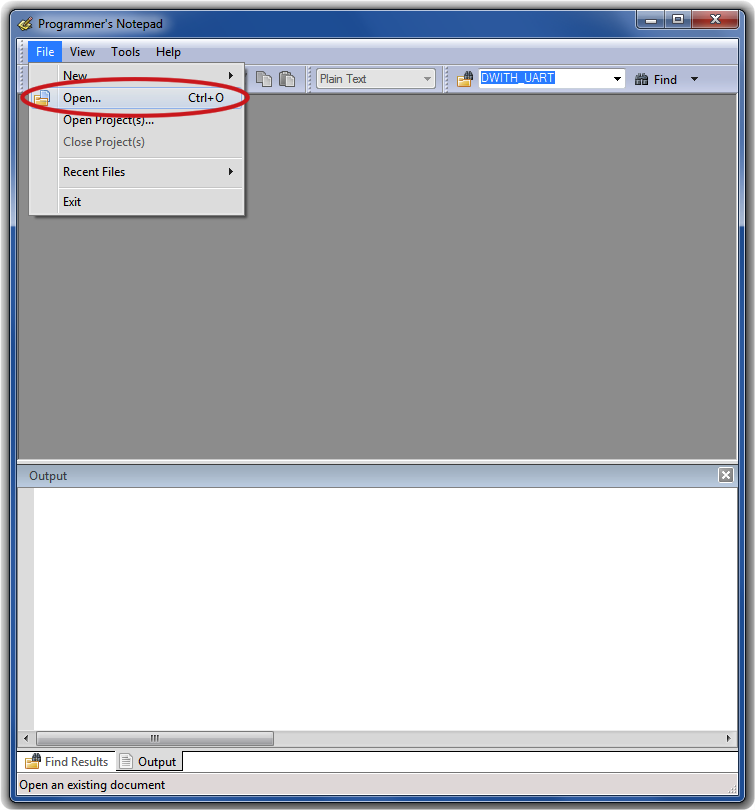
\includegraphics[width=.85\textwidth]{../PNG/Notepad_open.png}
    \caption{open Makefile}
  \end{subfigure}
  ~
  \begin{subfigure}[b]{.5\textwidth}
    \centering
    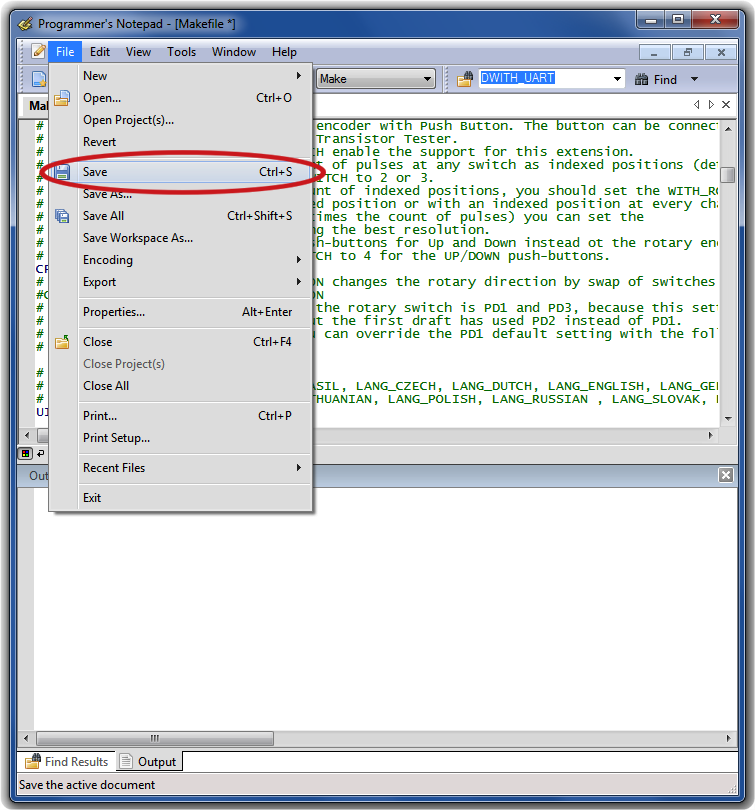
\includegraphics[width=.85\textwidth]{../PNG/Notepad_save.png}
    \caption{save Makefile}
  \end{subfigure}
  \caption{Bedienung der WinAVR-Oberfläche Programmer's Notepad}
  \label{fig:WinAVR1}
\end{figure}
Die Abbildungen \ref{fig:WinAVR1} zeigen das File-Menü der Bedienoberfläche von WinAVR zum
Öffnen der Datei \lname{Makefile} und zum Abspeichern der \lname{Makefile} nach den Änderungen (save).
\begin{figure}[H]
  \begin{subfigure}[b]{.5\textwidth}
    \centering
    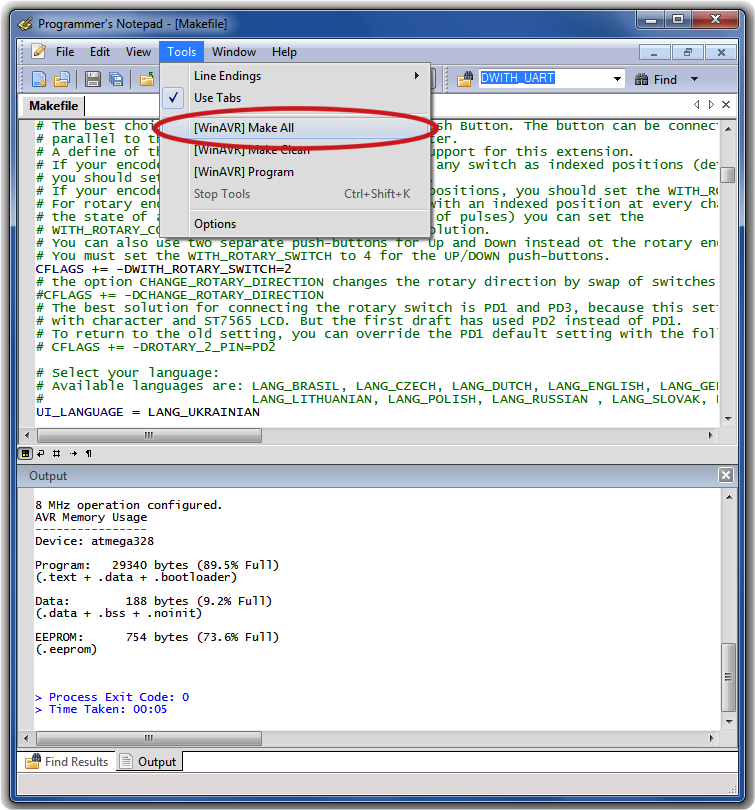
\includegraphics[width=.85\textwidth]{../PNG/Notepad_make.png}
    \caption{Erzeuge Programmdaten (.hex/.eep)}
  \end{subfigure}
  ~
  \begin{subfigure}[b]{.5\textwidth}
    \centering
    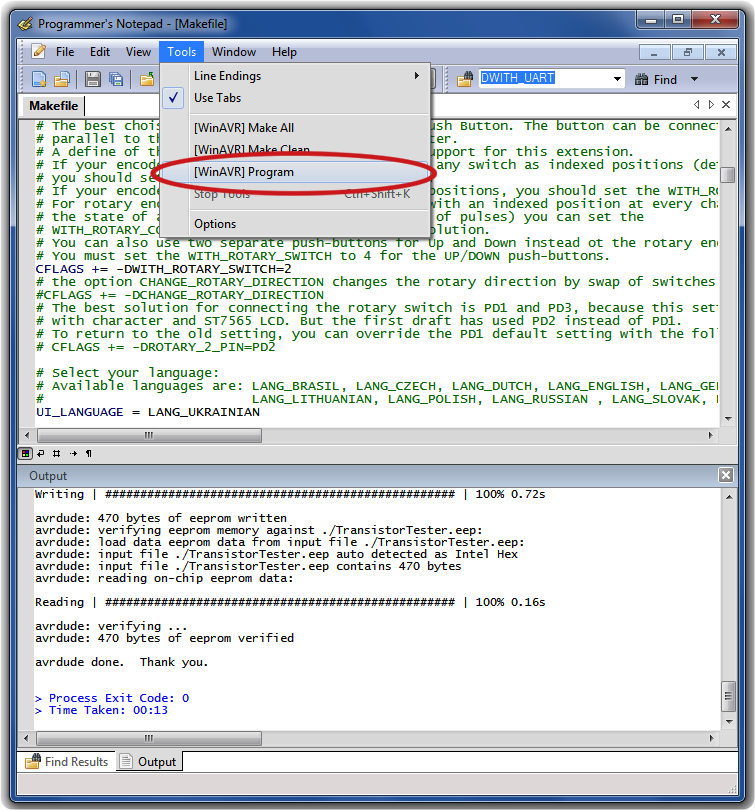
\includegraphics[width=.85\textwidth]{../PNG/Notepad_program.png}
    \caption{Programmiere ATmega}
  \end{subfigure}
  \caption{Bedienung der WinAVR-Oberfläche Programmer's Notepad}
  \label{fig:WinAVR2}
\end{figure}
Die nächsten Abbildungen \ref{fig:WinAVR2} zeigen das Tools-Menü von Programmer's Notepad
zum Übersetzen des Programms (Make All) und zum Programmieren des ATmega (Program) mit \lcmd{avrdude}.


\chapter{Popis metody měření}
\label{sec:measurement}
Zjednodušená schéma vstupu / výstupu ATmega je zobrazeno na obrázku~\ref{fig:port}.
Přepínač PUD vypne napájení pro všechny \inquotes{Pull Up} odpory ATmega.
Pomocí přepínače DD lze výstup vypnout, vstup pracuje bud jako výstup, tak i jako vstup.
Ve vstupním režimu je výstupní hodnota (PORT) použita k přepnutí \inquotes{Pull Up} odporu vstupu.
Ty dva přepínače PORT a DD nelze přepínat současně, ale pouze jeden po druhém.
Protože přepnutí \inquotes{Pull Up} odporu může rušit měření, dávám přednost úplnému
odpojení všech  \inquotes{Pull Up} odporů pomocí spínače PUD.
Samozřejmě, že jsou přepínače elektronické a odpory \(19\Omega\) a \(22\Omega\) jsou jen přibližné hodnoty.

\begin{figure}[H]
\centering
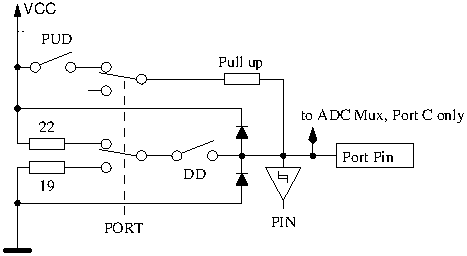
\includegraphics[width=.8\textwidth]{../FIG/port.pdf}
\caption{Zjednodušené schéma každého pinu ATmega portu}
\label{fig:port}
\end{figure}

Každý ze tří zkušebních pinů vašeho testeru se skládá ze tří pinů ATmega,
který je znázorněn na zjednodušeném schéma zkušebního čepu TP2 (prostřední ze tří pinů) na obrázku~\ref{fig:terminal}.

\begin{figure}[H]
\centering
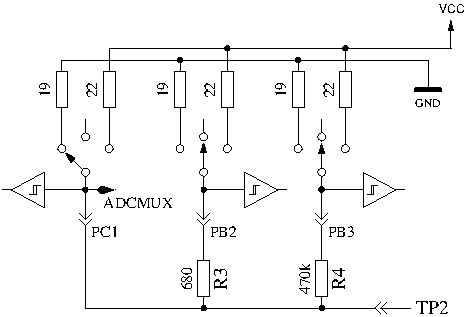
\includegraphics[width=.8\textwidth]{../FIG/terminal.pdf}
\caption{Zjednodušené schéma zapojení zkušebního pinu TP2}
\label{fig:terminal}
\end{figure}

Každý zkušební pin (měřící port) lze použít jako digitální nebo analogový vstup.
Tato schopnost měření je nezávislá na použití portu jako výstupu.
Každý zkušební pin může být použit jako výstup a připojen v tomto stavu k GND (\(0V\)) nebo VCC (\(5V\)),
nebo může být připojen buď k GND nebo VCC pomocí odporů (\(680\Omega\) nebo \(470k\Omega\)).
Tabulka \ref{tab:case} zobrazuje všechny možnosti měření.
Všimněte si, že pozitivní stav je dosažen připojením přímo k VCC (Port C) nebo
připojením k rezistoru \(680\Omega\) s VCC (Port B).
Stejná možnost má negativní stav zkušebního kolíku na straně GND.
Stav testu znamená, že pin může být otevřený (vstup) připojen pomocí odporu \(470k\Omega\) s VCC nebo GND,
nebo pin může být připojen k VCC nebo GND přes \(680\Omega\)-odpor.

\begin{table}[H]
  \begin{center}
    \begin{tabular}{| l | c | c | c |}
    \hline
      & Stav Pin 1 & Stav Pin 2 & Stav Pin 3 \\
    \hline
   1. & positivní    &  negativní   &  test \\
   2. & positivní    &  test      & negativní \\
   3. & test       &  negativní   & positivní \\
   4. & test       &  positivní   & negativní \\
   5. & negativní    &  test      & positivní \\
   6. & negativní    &  positivní   &  test  \\
    \hline
    \end{tabular}
  \end{center}
  \caption{všechny možnosti měření}
  \label{tab:case} 
\end{table}

Jakmile je nakonfigurováno měření kondenzátoru testerem,  pokusí se přístroj nejprve
k vybíjení kondenzátorů na všech připojovacích kolících.
Pokud to nefunguje, to znamená zbytkové napětí je příliš vysoké, bude vybíjení
po cca 12 sekundách přerušeno se zprávou \inquotes{Cell!}.

To se může stát i v případě když není žádný kondenzátor připojen.

Příčinou může v tomto případě být, že je mezní napětí výboje pro tento
ATmega příliš nízké.\\ Pomocí makefile volby CAP\_EMPTY\_LEVEL, můžete ale zvolit vyšší zbytkové napětí.


 %\newpage
\section{Messung von Halbleitern}
Als erster Test soll der Stromfluß des Bauteils bei stromlosen Steuerpin (dritter Pin, auch TriState-Pin genannt)
untersucht werden. Der Steuerpin ist beispielsweise das Gitter oder die Basis des Testobjektes.
Ein Testpin wird die positive Seite des Bauteils angenommen und direkt mit VCC verbunden.
Ein anderer Pin wird als negative Seite des Bauteils angenommen.
Die negative Seite wird mit dem \(680\Omega\) Widerstand nach GND verbunden.
Bei Feldeffekttransistoren ist der Zustand des Transistors von der Spannung des Gitters abhängig.
Der TriState-Pin wird zuerst mit dem \(680\Omega\)-Widerstand für \(5ms\) mit GND verbunden und
die Spannung an der negativen Seite gemessen.
Danach wird die Spannung des negativen Testpins wieder gemessen, während der TriState-Pin auf
Eingang (hochohmig) geschaltet ist.
Danach wird das angenommene Gate für \(5ms\) mit dem \(680\Omega\)-Widerstand auf VCC geschaltet 
und die Spannung an der negativen Seite noch einmal gemessen.
Wenn die gemessene Spannung jetzt niedriger ist als bei der ersten Messung, wird diese Schaltung
als richtig angenommen. Dann wird die Spannung noch einmal mit stromlosem Tristate-Pin gemessen.

Wenn die Spannung des negativen Pins mit festgehaltenem Pegel größer als \(115mV\) ist
und dieser Pegel nicht \(100mV\) niedriger als der Pegel mit stromlosen Tristate-Pin ist,
wird ein Verarmungs-Typ angenommen.
Bei bipolaren Transistoren mit hohem Reststrom ist
der Kollektor-Reststrom bei stromloser Basis deutlich höher.
Durch die Überprüfung beider Pegel wird eine Falschdetektion von Germanium-Transistoren mit
höheren Kollektor-Restströmen als Verarmungs-Transistoren (JFET) vermieden.
Es werden dann weitere Tests gemacht,
um N-Kanal JFET oder D-MOSFET und P-Kanal JFET oder P-MOSFET zu unterscheiden.
Die MOSFET-Versionen können erkannt werden durch das Fehlen von Steuerstrom in jedem 
TriState-Pin-Zustand.

Um Parameter der Verarmungstypen messen zu können, werden sie mit einem \(680\Omega\)-Widerstand am
Source-Pin vermessen, wie in Abbildung \ref{fig:JFETcd} gezeigt wird. Diese Messung wird anstelle der
üblichen Messung des Stromes bei einer Gate-Spannung auf Source-Potential gemacht, da wegen des
relativ hohen \(680\Omega\) Widerstandes in vielen Fällen der Kennstrom \(I_\mathrm{DSS}\) 
des FETs nicht erreicht würde.

\begin{figure}[H]
\centering
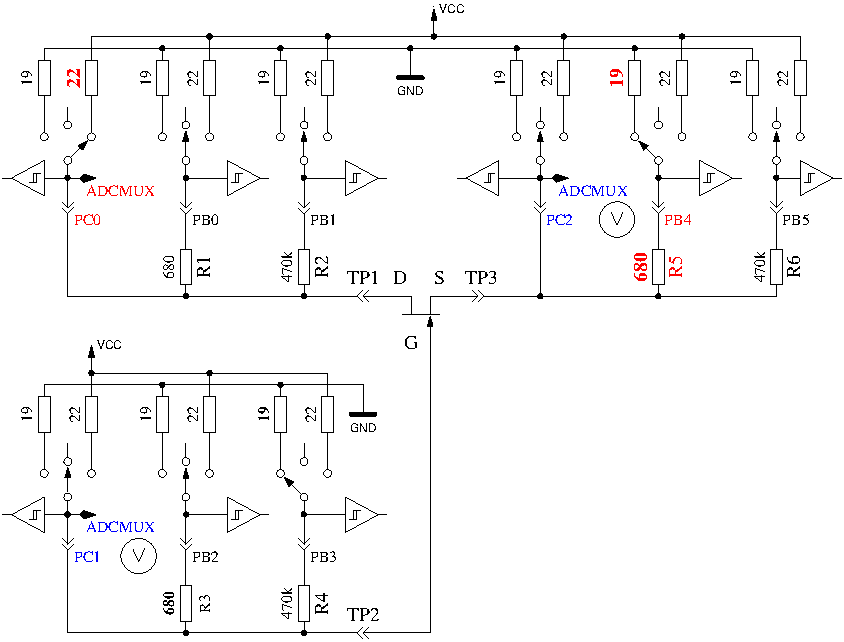
\includegraphics[width=.8\textwidth]{../FIG/JFETcd.pdf}
\caption{Messung von Gate-Source-Spannung und Source-Strom eines N-JFET-Transistors}
\label{fig:JFETcd}
\end{figure}

Wenn das Bauteil keinen Strom zwischen dem positiven Pin und dem negativen Pin ohne ein Signal
auf dem Tristate-Pin hat, sind die nächsten Tests im nächsten Unterkapitel \ref{sec:pnp} beschrieben.
Wenn Strom festgestellt wird, sind die nächsten Tests in dem Dioden-Unterkapitel \ref{sec:diode} beschrieben.

\subsection{Messung eines PNP-Transistors oder eines P-Kanal MOSFETs}
\label{sec:pnp}
Zuerst wird der Stromverstärkungsfaktor in der Kollektor-Schaltung (Emitter-Folger) für den angenommenen
PNP-Transistor gemessen.
Die Messsituation wird in Abbildung \ref{fig:pnpcc} gezeigt.
Wenn die gemessene Basis-Spannung (\(UB\)) über \(9mV\) mit dem \(680\Omega\) Widerstand liegt,
wird die Stromverstärkung hFE berechnet mit \(hFE = \frac{UE-UB}{UB}\). 
Die Spannung \(UE\) ist die Differenz der Emitter-Spannung zu VCC.
Die Differenz des \(22\Omega\) und \(19\Omega\)-Widerstandes wird nicht berücksichtigt.
Wenn die Spannung \(UB\) unter \(10mV\) liegt, wird die Messung mit dem \(470k\Omega\)-Widerstand an der Basis gemacht.
Für diesen Fall wird der Stromverstärkungsfaktor mit \(hFE = \frac{UE \cdot 470000}{UB \cdot (680+22)}\) gebildet.

\begin{figure}[H]
\centering
 \begin{overpic}[width=1.\textwidth]{../FIG/PNPcc.pdf}
  \color{black}
  \put(55,20){\makebox(0,0)[lb]{\footnotesize {Wenn Spannung an PC1 \textless~10mV ist,}}}
  \put(55,17){\makebox(0,0)[lb]{\footnotesize {wird der \textcolor{green}{grün} gezeichnete Zustand benutzt!}}}
 \end{overpic}
\caption{hFE-Messung eines PNP-Transistors in Kollektor-Schaltung}
\label{fig:pnpcc}
\end{figure}

Als Nächstes werden die Tests in Emitter-Schaltung für den angenommenen PNP-Transistor gemacht.
Die positive Seite wird jetzt direkt mit VCC verbunden, der \(680\Omega\)-Widerstand der negativen Seite wird 
mit GND verbunden, wie es in Abbildung \ref{fig:pnpce} gezeigt wird. 
Wenn die negative Seite des Bauteils eine Spannung über \(3,4V\) hat, wenn der \(680\Omega\)-Widerstand auf der Basis-Seite mit
GND verbunden ist, muss es ein PNP-Transistor oder ein P-Kanal-FET sein.
Das kann einfach unterschieden werden durch Prüfen der Basis-Spannung: Wenn sie grösser als \(0,97V\) ist, muss es ein PNP sein.
Für die Messung des Stromverstärkungsfaktors wird anstelle des \(680\Omega\)-Widerstandes der
 \(470k\Omega\)-Widerstand als Basis-Widerstand genommen.
Der Stromverstärkungsfaktor wird berechnet mit \(hFE = \frac{(UC-UC0) \cdot 470000}{UB \cdot (680+19)}\) .
Die Spannung UC0 ist die Spannung am Kollektorwiderstand ohne Basisstrom.
Der höhere Stromverstärkungsfaktor wird als der richtige angenommen, dieser hier oder der
mit der Kollektor-Schaltung bestimmte.


Die Werte, die für den PNP-Transistor herausgefunden wurden, sind nur gültig, wenn ein zweiter Satz
von Messungen gemacht wurde.
Um zu verhindern, dass der PNP-Transistor in der inversen Schaltung (Kollektor und Emitter vertauscht) erkannt
wird, wird dann die Messung mit dem höheren Stromverstärkungsfaktor als richtige Messung genommen.
Wenn die Basis-Spannung kleiner als \(0,97V\) ist, muss es ein P-E-MOS sein.
In diesem Fall wird die Gate-Schwellwertspannung dadurch bestimmt, dass die Spannung am Gate langsam mit dem
 \(470k\Omega\)-Widerstand rauf und runter gezogen wird, bis die Drain-Seite schaltet und dann
die Spannung am Gate gemessen wird.

\begin{figure}[H]
\centering
 \begin{overpic}[width=1.\textwidth]{../FIG/PNPce.pdf}
  \color{black}
  \put(55,21){\makebox(0,0)[lb]{\footnotesize {Schwarzer Zustand wird benutzt beim Test!}}}
  \put(55,17){\makebox(0,0)[lb]{\footnotesize {\textcolor{green}{Grüner} Zustand wird für den}}}
  \put(55,13){\makebox(0,0)[lb]{\footnotesize {Stromverstärkungsfaktor hFE benutzt.}}}
 \end{overpic}
\caption{Prüfung und hFE-Messung eines PNP-Transistors in der Emitter-Schaltung}
\label{fig:pnpce}
\end{figure}

\subsection{Messung eines NPN-Transistors oder eines N-Kanal-MOSFET}
Die Messung eines NPN-Transistors beginnt auf gleiche Weise wie die PNP-Transistor-Messung, nämlich
mit der Messung des Stromverstärkungsfaktors in der Kollektor-Schaltung.
Zuerst wird die Messung mit einem nach VCC geschalteten \(680\Omega\)-Basiswiderstand gemacht.
Wenn die Spannung am Basis-Widerstand zu klein ist, wird stattdessen der \(470k\Omega\)-Widerstand genommen.
Die Messungen werden dann in der Emitter-Schaltung fortgeführt, wie in Abbildung \ref{fig:npnce} gezeigt.
\begin{figure}[H]
\centering
 \begin{overpic}[width=1.\textwidth]{../FIG/NPNce.pdf}
  \color{black}
  \put(55,23){\makebox(0,0)[lb]{\footnotesize {Schwarzer Zustand wird benutzt beim Test!}}}
  \put(55,19){\makebox(0,0)[lb]{\footnotesize {\textcolor{green}{Grüner} Zustand wird für den}}}
  \put(55,15){\makebox(0,0)[lb]{\footnotesize {Stromverstärkungsfaktor hFE benutzt.}}}
 \end{overpic}
\caption{Prüfung und hFE-Messung eines NPN-Transistors in Emitter-Schaltung}
\label{fig:npnce}
\end{figure}
Wenn die Spannung auf der Kollektor Seite unter \(1,6V\) liegt, während der \(680\Omega\)-Basiswiderstand mit
VCC verbunden ist, muss es ein NPN, ein N-Kanal MOSFET oder ein Thyristor (TRIAC) sein.
Mit zwei einfachen Tests kann ein Thyristor oder TRIAC erkannt werden.
Wenn der Gate-Pin für \(10ms\) mit GND verbunden wird und dann stromlos geschaltet wird, sollte
der Strom an der Anode bleiben.
Wenn jetzt der Anoden-Widerstand kurz auf GND geschaltet und dann auf VCC zurückgeschaltet wird,
sollte der Thyristor nicht erneut zünden (stromlos bleiben).
Beachten Sie, dass nur Kleinleistungs-Thyristoren getestet werden können, weil der Haltestrom des
Testers nur \(6mA\) erreichen kann.
Wenn beide Tests einen Thyristor bestätigen, werden weitere Tests in umgekehrter Polarität gemacht,
um ein TRIAC auszuschliessen oder zu bestätigen.

Wenn weder Thyristor noch TRIAC bestätigt wurden, kann es ein NPN oder ein N-Kanal E-MOSFET sein.
Die Basis-Spannung von einem NPN-Transistor wird nahe bei der Emitter-Spannung liegen, so dass dieser Typ sicher
erkannt werden kann.
Der Stromverstärkungsfaktor in der Emitter-Schaltung wird durch 
\(hFE = \frac{(VCC-UC-UC0)\cdot 470000}{(VCC-UB)\cdot (680+22)}\) gebildet.
Wenn die Spannung an der Basis zeigt, dass kein oder wenig Strom fließt, wird das Bauteil ein N-Kanal E-MOS
(Anreicherungs-MOSFET) sein.
In diesem Fall wird die Schwellspannung gemessen, indem die Spannung des Gates langsam mit
dem \(470k\Omega\)-Widerstand nach VCC und GND gezogen wird, darauf wartend, dass das digitale
Eingangs-Signal auf der Drain-Seite schaltet, wobei dann die Gate-Spannung gelesen wird.
Die Messung wird elf Mal wiederholt wie in Abbildung~\ref{fig:eleven} gezeigt und die Ergebnisse addiert.
Diese Summe wird mit Vier multipliziert und durch Neun geteilt, um eine Auflösung in mV zu erhalten.
\begin{figure}[H]
\centering
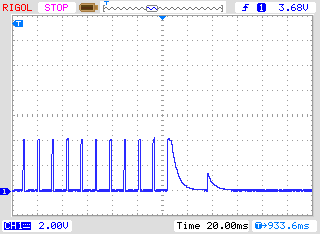
\includegraphics[width=.8\textwidth]{../PNG/IRFU120gate.png}
\caption{Messung der Schwellspannung eines N-Kanal-MOSFET}
\label{fig:eleven}
\end{figure}

\subsection{Vereinfachter Ablauf der Transistorerkennung}

\begin{figure}[H]
\centering
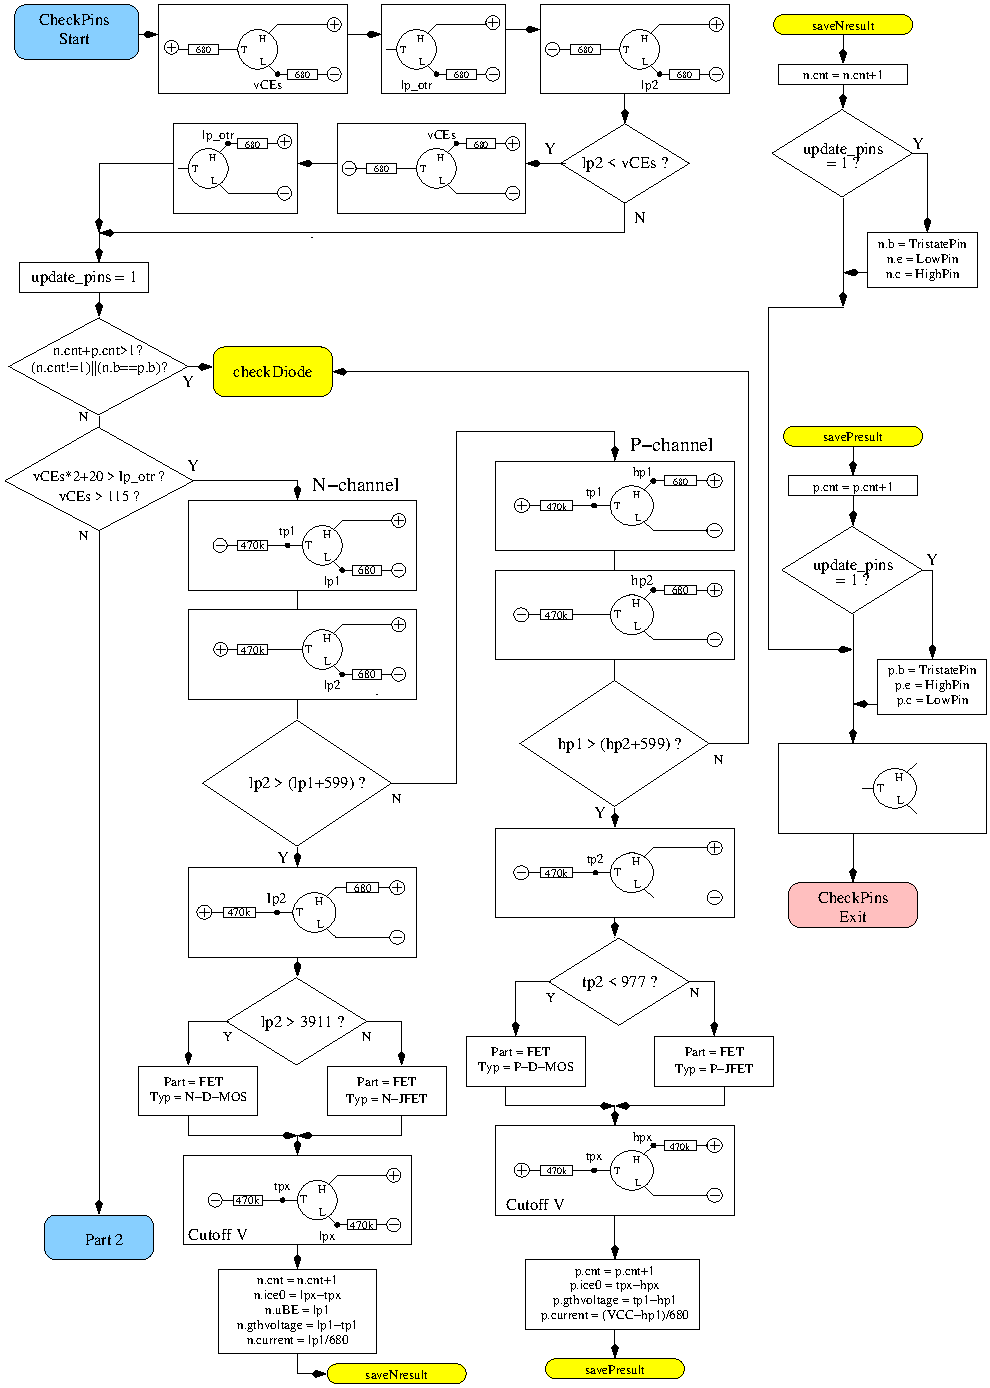
\includegraphics[width=.95\textwidth]{../FIG/CheckSemi1.pdf}
\caption{Ablaufplan der Transistorprüfung Teil 1, JFET und D-MOS}
\label{fig:ChkSemi1}
\end{figure}

\begin{figure}[H]
\centering
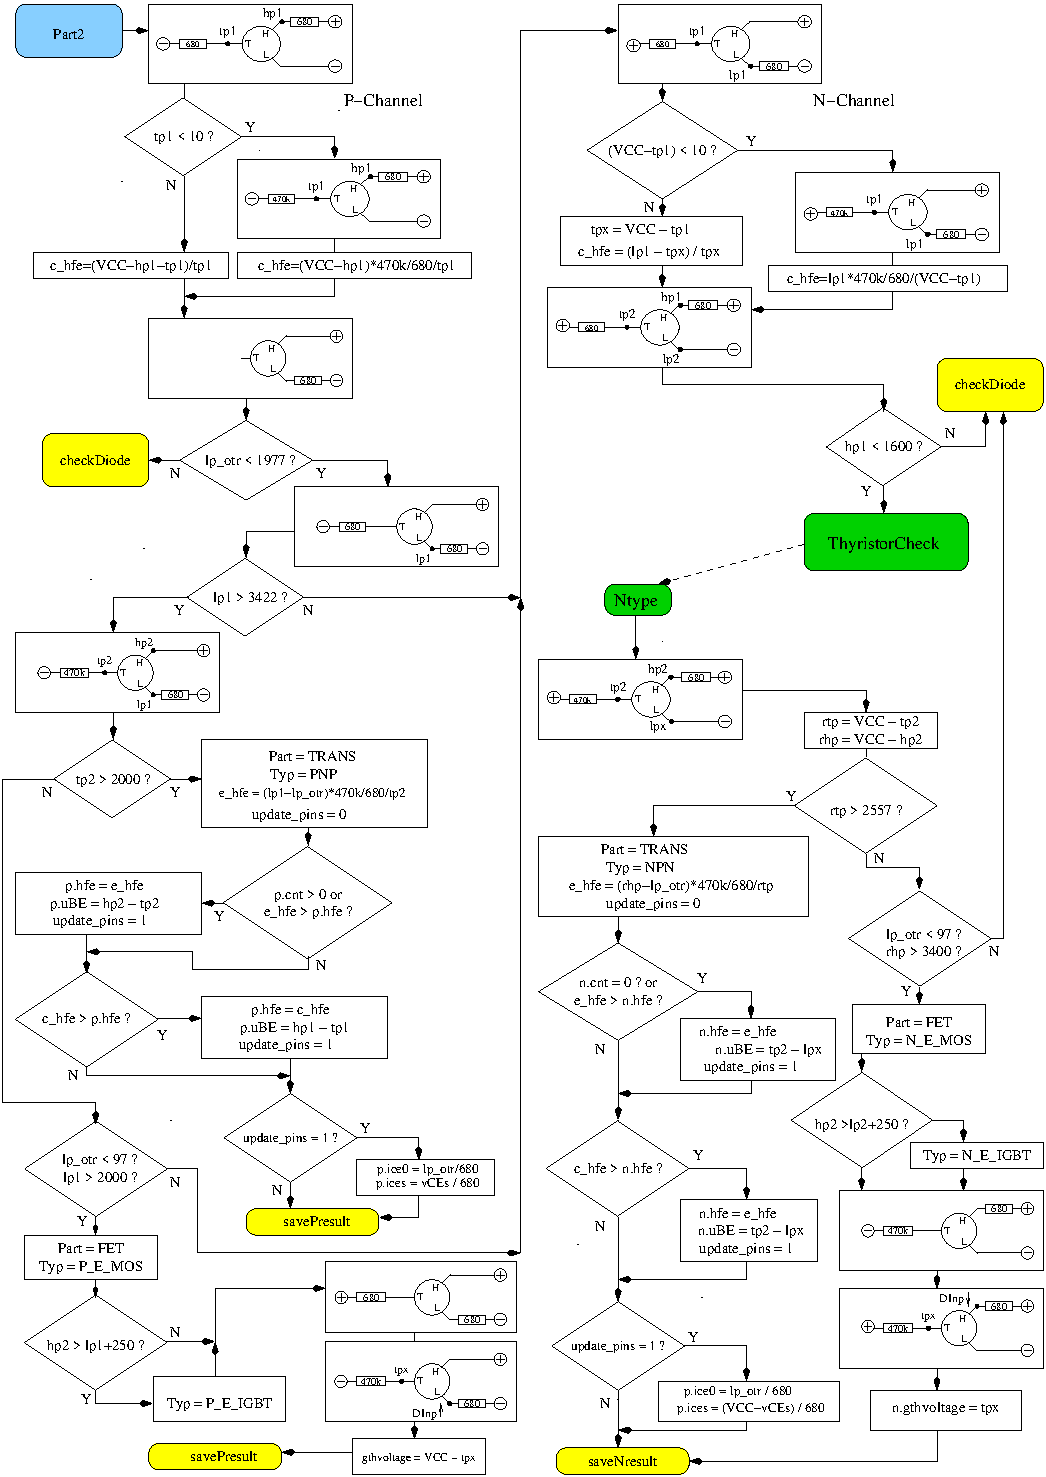
\includegraphics[width=.95\textwidth]{../FIG/CheckSemi2.pdf}
\caption{Ablaufplan der Transistorprüfung Teil 2, BJT und E-MOS}
\label{fig:ChkSemi2}
\end{figure}

\begin{figure}[H]
\centering
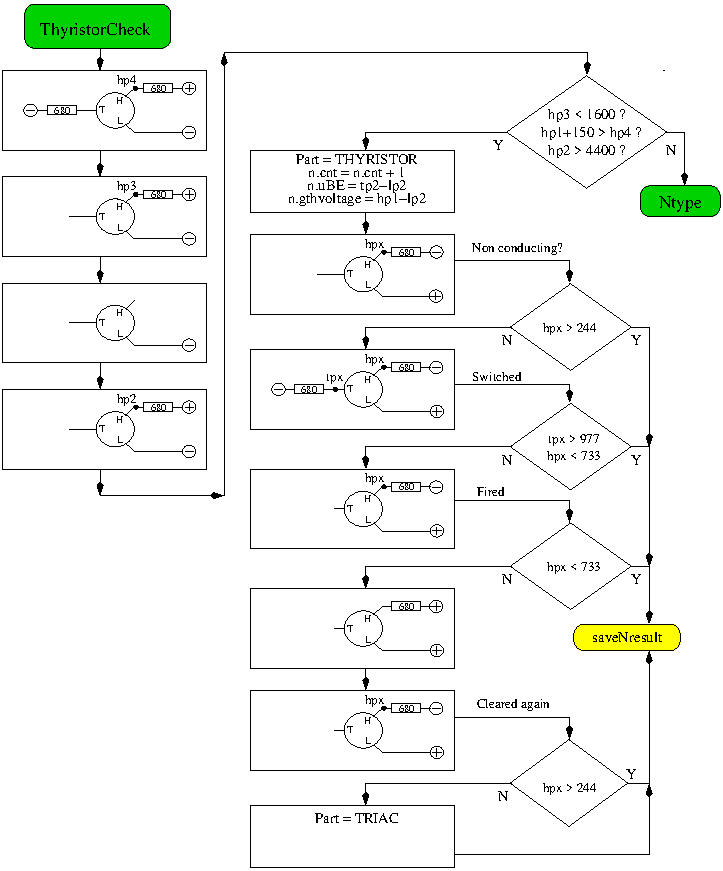
\includegraphics[width=.95\textwidth]{../FIG/CheckSemi3.pdf}
\caption{Ablaufplan der Transistorprüfung Teil 3, Thyristor und Triac}
\label{fig:ChkSemi3}
\end{figure}

\subsection{Messung von Dioden}
\label{sec:diode}
Wenn Strom bei den Vortests festgestellt wurde, wird das Bauteil auf Diodenverhalten geprüft.
Die Flussspannung mit dem \(680\Omega\)-Widerstand muss zwischen \(0,15V\) und \(4,64V\) liegen.
Die Flussspannung mit dem \(680\Omega\)-Widerstand muss grösser als 1,125 Mal der Flussspannung mit dem
 \(470k\Omega\)-Widerstand sein und sechzehn Mal die Flussspannung mit dem \(470k\Omega\)-Widerstand muss
grösser als die Flussspannung mit dem \(680\Omega\)-Widerstand sein.
Zusätzlich darf die anschließende nochmalige Messung mit dem \(470k\Omega\)-Widerstand keine höhere Spannung als die
Messung mit dem \(680\Omega\)-Widerstand ergeben.
Ich hoffe, dass ein Bauteil mit diesem Verhalten immer eine Diode ist.
Die Erkennung des Diodenverhaltens durch den fehlenden Stromfluß in der Gegenrichtung ist nicht
möglich bei antiparallelen Dioden.
Bei einer Einzeldiode wird zusätzlich der Sperrstrom der Diode bei \(5V\) mit dem \(470k\Omega\) Widerstand
gemessen. Die Auflösung beträgt etwa \(2nA\).
Bei größeren Restströmen als \(5,3\mu A\) (Spannung am Widerstand größer als \(2,5V\)) wird
 mit dem \(680\Omega\) Widerstand gemessen.
Dann beträgt die Auflösung nur etwa \(1\mu A\).
Außerdem wird bei Einzeldioden eine Kapazitätsmessung in Sperr-Richtung durchgeführt. 

\subsection{Ergebnisse der verschiedenen Messungen}
Die folgenden drei Tabelle zeigen die Ergebnisse verschiedener Bauteile 
eines ATmega8-, ATmega168- und ATmega328-Prozessors.
Die Messung der Sperrschichtkapazität für die Doppeldiode MBR4045PT gelingt
nur gekühlt. Die Ursache hierfür ist der hohe Reststrom der \(40A\)-Diode. Ebenso kann für die Basis-Emitter-Strecke 
des Germanium-Transistors AC128 die Sperrschichtkapazität nur im
gekühlten Zustand gemessen werden. 

\begin{table}[H]
  \begin{center}
    \begin{tabular}{| l | c | c | c | c |}
    \hline
           & Mega8@8MHz          & Mega168 @8MHz       & Mega328 @8MHz     \\
 Diode Typ &                     &                     &                   \\
    \hline
    \hline
1N4148     & Diode, 715mV,        & Diode, 718mV,            & Diode, 715mV,           \\
           &               1pF    &               0pF, 2nA   &               1pF, 4nA  \\
    \hline
1N4150     & Diode, 665mV,        & Diode, 672mV,            & Diode, 666V,           \\
           &               1pF    &               1pF, 4nA   &              2pF, 6nA  \\
    \hline
BA157      & Diode, 619mV,        & Diode, 621V,              & Diode, 615mV,            \\
           &               19pF   &              17pF, 12nA   &               18pF, 12nA \\
    \hline
BY398      & Diode, 538mV,        & Diode, 541mV,             & Diode, 537mV,            \\
           &               16pF   &               14pF, 63nA  &               15pF, 63nA \\
    \hline
1N4007     & Diode, 650mV,        & Diode, 655mV,            & Diode, 650mV,           \\
           &               13pF   &               10pF, 6nA  &               13pF, 6nA \\
    \hline
LED green  & Diode, 1.96V, 5pF    & Diode, 1.95V, 4pF   & Diode, 1.95V, 4pF \\
    \hline
ZPD2,7     & 2xDi, 743mV, 2.53V   & 2xDi, 737mV, 2.52V  & 2xDi, 733mV, 2.51V \\
    \hline
BU508A B+E & Diode, 609mV,        & Diode, 611mV,                & Diode, 606mV,              \\
           &               5.15nF &               5.20nF, 0.39uA &               5.25nF, 0.4uA\\
    \hline
BU508A B+C & Diode, 582mV,        & Diode, 586mV,             & Diode, 587mV,            \\
           &               256pF  &               255pF, 21nA &               259pF, 19nA\\
    \hline
AC128 B+E  & Diode, 272mV,        & Diode, 277mV,              & Diode, 273mV,             \\
           &               0pF    &               0pF, 2.2uA   &               0pF, 2.3uA  \\
    \hline
AC128 B+E  &                      &                     & Diode, 349mV,               \\
gekühlt    &                      &                     &               140pF, 0.57uA \\
    \hline
MBR20100CT & 2xDi, 337mV, 337mV   & 2xDi, 338mV, 338mV  & 2xDi, 336mV, 335mV  \\
    \hline
MBR20100CT & Diode, 337mV,        & Diode, 339mV,             & Diode, 337mV,            \\
           &               345pF  &               351pF, 29nA &               350pF, 25nA\\
    \hline
MBR4045PT  & Diode, 243mV,        & Diode, 233mV,               & Diode, 235mV,              \\
gekühlt    &               1.80nF &               1.94nF, 1.7uA &               1.95nF, 1.8uA\\
    \hline
SK14       & Diode,    mV,        & Diode,    mV,               & Diode, 263mV,              \\
           &                  0pF &                   pF,    nA &               0pF, 0.57uA\\
    \hline
SK14       & Diode,    mV,        & Diode,    mV,               & Diode, 334mV,              \\
gekühlt    &                   nF &                   pF,    nA &               88pF, 4nA\\
    \hline
SF38G      & Diode, 519mV,        & Diode, 521mV,            & Diode, 516mV,            \\
           &               107pF  &               105pF, 2nA &               106pF, 2nA \\
    \hline
    \end{tabular}
  \end{center}
  \caption{Messergebnisse der Dioden-Tests}
  \label{tab:diodes} 
\end{table}

\begin{table}[H]
  \begin{center}
    \begin{tabular}{| l | c | c | c | c | c |}
    \hline
 Transistor & Typ & Mega8           & Mega328        & Mega328         & Mega328 \\
    Typ     &     & common-         & maximum        & common-         & common- \\
            &     & collector       &                & collector       & emitter \\
    \hline
    \hline
BU508A      & NPN & B=9, 601mV      &  B=9, 597mV    &   B=9, 598mV    & B=4, 484mV \\
    \hline
2N3055      & NPN & B=20, 557mV     &  B=21, 550mV   &   B=21, 550mV   & B=6, 442mV \\
    \hline
BC639       & NPN & B=148, 636mV    &  B=172, 629mV  &   B=172, 629mV  & B=158, 605mV \\
    \hline
BC640       & PNP & B=226, 650mV    &  B=176, 609mV  &   B=171, 655mV  & B=177, 608mV \\
    \hline
BC517       & NPN & B=23.9k, 1.23V  &  B=24.8k, 1.22V&   B=25.1k, 1.22V & B=764, 1.23V \\
    \hline
BC516       & PNP & B=75.9k, 1.21V  &  B=76.2k, 1.20V&   B=76.2k, 1.20V & B=760, 1.23V \\
    \hline
BC546B      & NPN & B=285, 694mV    &  B=427, 687mV  &   B=427, 687mV   & B=369, 683mV \\
    \hline
BC556B      & PNP & B=304, 704mV    &  B=254, 668mV  &   B=235, 709mV   & B=255, 668mV \\
    \hline
AC128 (Ge.) & PNP & B=63, 191mV     &  B=59, 191mV   &   B=57, 193mV    & B=43, 117mV \\
    \hline
BUL38D      & NPNp & B= 37, 627mV    &  B=41, 617mV  &   B=40, 624mV    & B=36, 562mV \\
parasitär   & PNPn & B= 11, 654mV    &  B=81, 543mV  &   B=10, 656mV    & B=83, 541mV \\
    \hline
BRY55/200   & Thyrist. &  0.84V      &  0.81V        &  0.82V           &  0.82V \\
    \hline
MAC97A6     & Triac &   0.92V        &  0.90V        &  0.91V           &  0.90V    \\
    \hline
    \end{tabular}
  \end{center}
  \caption{Messergebnisse der Tests mit bipolaren Transistoren}
  \label{tab:bipolar} 
\end{table}

Die Ergebnisse der Transistormessungen unterscheiden sich teilweise erheblich von den Werten der Version 
von Markus Frejek. Zum Beispiel wird für den Darlington-Transistor BC517 von
der früheren Software ein hFE von nur 797 statt 77200 gemessen. 
Dies hängt damit zusammen, dass die Stromverstärkung bei der neuen Version auch mit der
Kollektorschaltung gemessen wird.
Dies zeigen auch die Ergebnisse der neuen Version in der Emitterschaltung (common emitter),
wie man in der letzten Spalte der Tabelle \ref{tab:bipolar} sehen kann.
Die Basis-Emitter-Spannung wurde früher mit einem separaten Diodentest mit \(1438mV\) ermittelt.
Jetzt wird die angegebene Basis-Emitter-Spannung im Zustand der Verstärkungsmessung (\(1,20V\)) ermittelt.
Der BUL38D-Transistor enthält eine Schutzdiode über der Anode und dem Kollektor des NPN-Transistors,
wodurch ein parasitärer PNP-Transistor mit vertauschtem Basis-Kollektor Anschluss entsteht.
In der Softwareversion 1.10k werden beide Transistoren erkannt und durch das angehängte p auf
den weiteren Transistor hingewiesen.
Der richtige Transistor (NPN) wird durch einen Vergleich der Sperrschichtkapazitäten herausgefunden.
Es wird angenommen, dass der mit der höheren Sperrschichtkapazität der richtige Transistor ist.
Wenn während der Ergebnisanzeige die Start-Taste gedrückt ist, werden die Parameter des parasitären Transistors
angezeigt. Dabei wird wieder mit PNPn auf die andere Transistorstruktur hingewiesen.
Die weitere Transistorstruktur entsteht nur bei der Integration der Schutzdiode in unmittelbarer
Nachbarschaft des Transistors in das gleiche Halbleitermaterial, nicht bei einer externen Diode.

In der folgenden Tabelle \ref{tab:germanium} werden die Messergebnisse von Germanium-Transistoren gezeigt, die wegen den
stark temperaturabhängigen Kollektor-Restströmen besonders problematisch sind.
Es werden die Ergebnisse der Urversion von Markus F. und die Ergebnisse der 1.10k Version
miteinander verglichen. Die 1.10k Version mißt die Stromverstärkung sowohl in der
Kollektorschaltung als auch in der Emitterschaltung mit Berücksichtigung des Kollektor-Ruhestroms,
 wobei die höhere Stromverstärkung ausgegeben wird.
Der Kollektor-Ruhestrom wurde in älteren Versionen nicht berücksichtigt.

\begin{table}[H]
  \begin{center}
    \begin{tabular}{| l | c | c | c |}
    \hline
 Transistor & Mega8 @1MHz          & Mega168 @8MHz       & Mega328 @8MHz    \\
    Typ     & Ur-Version          & Version 1.10k       & Version 1.10k  \\
            & Markus F.           &                     &        \\
    \hline
    \hline
AC128       & PNP, B=52, 279mV    & PNP, B=59, 184mV    & PNP, B=59, 191mV    \\
    \hline
AC116-65    & PNP, B=505, 378mV   & PNP, B=72, 146mV    & PNP, B=72, 149mV    \\
    \hline
AC116-145   & PNP, B=485, 294mV   & PNP, B=146, 161mV    & PNP, B=146, 163mV   \\
    \hline
AC176-65    & NPN, B=98, 235mV    & NPN, B=58, 94mV    & NPN, B=56, 96mV     \\
    \hline
GC122       & PNP, B=84, 368mV    & PNP, B=55, 117mV    & PNP, B=56, 117mV    \\
    \hline
GC301       & PNP, B=48, 289mV    & PNP, B=39, 184mV    & PNP, B=39, 188mV    \\
    \hline
AD161       & NPN, B=360, 230mV   & NPN, B=296, 126mV   & NPN, B=298, 128mV    \\
    \hline
AD162       & PNP, B=2127, 280mV  & PNP, B=89, 107mV    & PNP, B=89, 107mV    \\
    \hline
    \end{tabular}
  \end{center}
  \caption{Messergebnisse der Tests mit bipolaren Germanium-Transistoren}
  \label{tab:germanium} 
\end{table}

In der Tabelle \ref{tab:mos} werden die Ergebnisse einiger Feldeffekttransistoren-Messungen gezeigt.
Ein gemessenen Parameter der E-MOS-Typen ist Gate-Source-Schaltspannung,
bei der das digitale Eingangssignal des ATmega eines am \(680\Omega\) Drain-Widerstand 
angeschlossenen Signals schaltet.
Bei sehr schneller Änderung der Gatespannung wegen einer kleinen Gatekapazität 
ist die ermittelte Spannung etwas ungenau.
Beim BS250 ändert sich die Gatespannung von \(2,6V\) auf \(2,5V\), wenn man einen zusätzlichen
\(10nF\) Kondensator an Gate-Source anschließt.

Ein anderer gemessener  Parameter ist die Gatekapazität.
Die Gatekapazität wird ermittelt indem sowohl Source als auch Drain auf GND Potential gelegt wird.
Bei IGBTs reicht oft die Gatespannung von \(5V\) des Testers nicht zur Ansteuerung aus.
Meistens wird dann nur die Emitter-Kollektor Schutzdiode erkannt. 
In diesem Fall kann eine an den Gatepin angeschlossene Batterie mit etwa \(3V\) reichen,
um die Erkennung zu ermöglichen. Der andere Pol der Batterie wird dann anstelle des Gatepins
an den Testpin (TP) des Testers angeschlossen.
Bei richtiger Polarität der Batterie wird dann die Erkennung des IGBTs ermöglicht.
Die angezeigte Gate-Emitter Schaltspannung muß dann um die Batteriespannung erhöht werden,
um die wahre Schaltspannung zu erhalten.

Bei JFET-Transistoren wird in den Datenblättern oft der Idss-Kennstrom genannt,
der Strom im Drain bei einer Gate-Source-Spannung von 0V.
Hier wird aber der Strom angegeben, der sich durch einen \(680\Omega\) Lastwiderstand auf der
Source-Seite des JFET ergibt.
Der Lastwiderstand erzeugt für das Gate eine Gegenspannung Vgs,
die ebenfalls angegeben wird.
Mit einem \(470k\Omega\) Lastwiderstand auf der Source-Seite des JFET ist der Source-Drain Strom
fast 0. Damit läßt sich die Gate-Source Cutoff Spannung Vgs\_off hinreichend genau bestimmen,
sofern sie unter \(5V\) liegt.
Mit diesen beiden Arbeitspunkten läßt sich aufgrund der quadratischen Strom-Kennlinie ein Igss
schätzen. Sofern der geschätzte Strom unter \(40mA\) liegt, wird noch eine zusätzliche Messung
ohne Widerstand am Source Anschluß gemacht. 
Über die Spannung am Source-Anschluß kann ein weiterer Stromwert bestimmt werden. 
Mit diesem höheren Stromwert und der Gate-Source Spannung wird der Strom Idss noch einmal mit
der quadratischen Strom-Kennlinie berechnet, sofern ein Wert von \(40mA\) nicht überschritten wird.
Wegen des symmetrischen Aufbaus der JFETs kann Drain und Source nicht unterschieden werden.

\begin{table}[H]
  \begin{center}
    \begin{tabular}{| l | l | c | c | c |}
    \hline
             &         & Mega8 @8MHz       & Mega168 @8MHz    & Mega328 @8MHz \\
 Transistor  & Typ     &                  &                  &               \\
    \hline
    \hline
ZVNL120A     & N-E-MOS & D, 1.6V, 147pF   & D, 1.5V,141pF    & D, 1.5V, 140pF \\
    \hline
IRF530N      & N-E-MOS & D, 3.6V, 1.55nF  & D, 3.6V, 1.54nF  & D, 3.6V, 1.54nF \\
    \hline
BS170        & N-E-MOS & D, 2.6V, 78pF    & D, 2.6V, 68pF    & D, 2.6V, 68pF \\
    \hline
IRL3803      & N-E-MOS & D, 2.3V, 9.81nF  & D, 2.3V, 9.71nF  & D, 2.3V, 9.74nF \\
    \hline
IRFU120N     & N-E-MOS & D, 4.2V, 909pF   & D, 4.2V, 913pF   & D, 4.2V, 911pF \\
    \hline
BUZ71A       & N-E-MOS & D, 3.2V, 714pF   & D, 3.2V, 708pF   & D, 3.2V, 705pF \\
    \hline
ZVP2106A     & P-E-MOS & D, 3.2V, 122pF   & D, 3.2V,115pF    & D, 3.2V, 116pF \\
    \hline
IRF5305      & P-E-MOS & D, 3.6V, 2.22nF  & D, 3.6V, 2.22nF  & D, 3.6V, 2.22nF \\
    \hline
BS250        & P-E-MOS & D, 2.6V, 53pF    & D, 2.6V, 43pF    & D, 2.6V, 44pF \\
    \hline
IRFU9024     & P-E-MOS & D, 3.5V, 937pF   & D, 3.6V, 945pF   & D, 3.5V, 933pF \\
    \hline
J310         & N-JFET  & 3.1mA Vgs=2.2V   & 3.1mA Vgs=2.2V   & 3.1mA Vgs=2.2V \\
Idss=24-60mA &         &                  &                  & Idss=35mA      \\
    \hline
2N5459       & N-JFET  & 2.1mA Vgs=1.5V   & 2.1mA Vgs=1.5V   & 2.1mA Vgs=1.5V \\
Idss=4-16mA &          &                  &                  & Idss=8.2mA     \\
    \hline
BF256C       & N-JFET  & 3.4mA Vgs=2.4V   & 3.4mA Vgs=2.4V   & 3.4mA Vgs=2.4V \\
Idss=11-18mA &         &                  &                  & Idss=14mA      \\
    \hline
BF245A       & N-JFET  & 1.1mA Vgs=.75V   & 1.1mA Vgs=0.75V  & 1.1mA Vgs=0.75V \\
Idss=2-6mA   &         &                  &                  & Idss=3.6mA      \\
    \hline
BF245B       & N-JFET  & 2.5mA Vgs=1.7V   & 2.5mA Vgs=1.7V   & 2.5mA Vgs=1.7V \\
Idss=6-15mA  &         &                  &                  & Idss=10mA      \\
    \hline
BF245C       & N-JFET  & 3.9mA Vgs=2.7V   & 3.9mA Vgs=2.7V   & 3.9mA Vgs=2.7V \\
Idss=12-25mA &         &                  &                  & Idss=17mA    \\
    \hline
J175        & P-JFET   & 3.2mA Vgs=2.2V   & 3.2mA Vgs=2.2V   & 3.2mA Vgs=2.2V \\
Idss=7-60mA &          &                  &                  & Idss=26mA      \\
    \hline
2N5460      & P-JFET   & 0.78mA Vgs=0.54V & 0.77mA Vgs=0.54V & 0.78mA Vgs=0.54V \\
Idss=1-5mA  &          &                  &                  & Idss=2.6mA       \\
    \hline
BSS139      & N-D-MOS  & 1.7mA Vgs=1.2V  & D, 1.7mA Vgs=1.2V & D, 1.7mA Vgs=1.2V \\
    \hline
BSS169      & N-D-MOS  & 2.6mA Vgs=1.8V  & D, 2.6mA Vgs=1.8V & D, 2.6mA Vgs=1.8V \\
    \hline
GP07N120    & N-E-IGBT & C=3.81nF Vt=4.2V & C=3.76nF Vt=4.2V & C=3.74nF Vt=4.2V \\
    \hline
IRG4PC30    & N-E-IGBT &                  &                  & C=2.22nF         \\
mit Bat.    &          &                  &                  & Vt=2.0V+3.2V \\
    \hline
    \end{tabular}
  \end{center}
  \caption{Messergebnisse der FET-Tests}
  \label{tab:mos} 
\end{table}

 %\newpage
\section{Měření odporů}
Každý odpor se měří čtyřmi měřicími metodami v jednom směru proudu.
Stejný odpor je měřen stejnými čtyřmi měřicími metodami v druhém směru proudu.
Měření v opačném směru se používá pouze pro detekci odporu.
Pokud je odchylka těchto dvou měření příliš velká, není to žádný odpor.

\subsection{Měření odporů s pomocí \(680\Omega\) odporů}
Měření neznámého odporu Rx se provádí dvěma různými způsoby s přesnými odpory \(680\Omega\).
Schéma zapojení těchto měření pomocí zkušebního kolíku 1 (TP1) a zkušebního kolíku 3 (TP3)
je zjednodušeně znázorněno na obr.~\ref{fig:RL1mes} a obrázku~\ref{fig:RL2mes} jako příklad
šesti možných kombinací.

\begin{figure}[H]
\centering
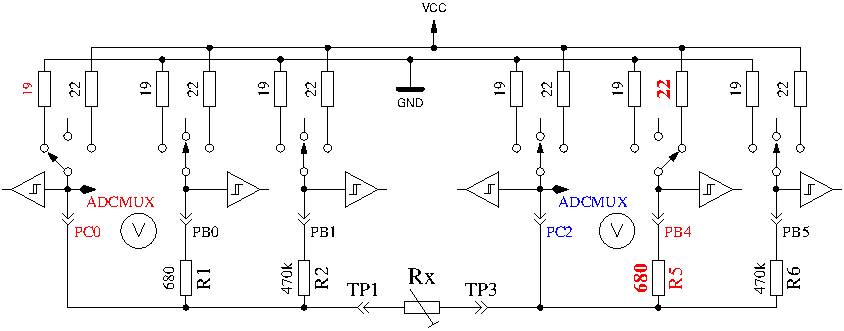
\includegraphics[width=.8\textwidth]{../FIG/ResistormessL1.pdf}
\caption{Měření typu 1 s \(680\Omega\) }
\label{fig:RL1mes}
\end{figure}

\begin{figure}[H]
 \centering
 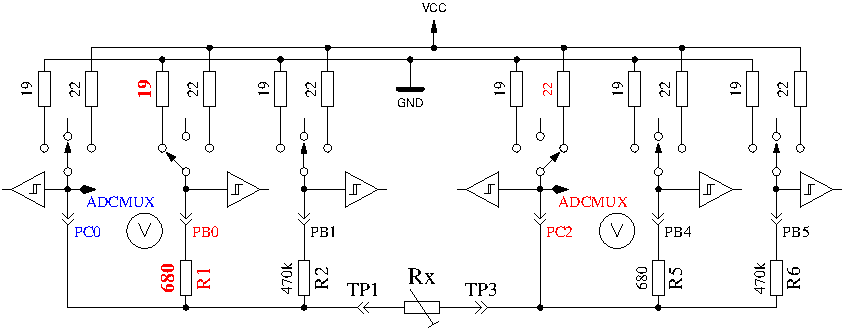
\includegraphics[width=.8\textwidth]{../FIG/ResistormessL2.pdf}
 \caption{Měření typu 2 s \(680\Omega\) }
\label{fig:RL2mes}
\end{figure}

Zkušební pin TP 1 je zobrazen na levé straně a zkušební pin TP 3 na pravé straně.
V obou obvodech je vidět, že je port 3 (TP3) spínán k VCC a na levé straně (TP1)
je připojen na zem GND.
Aktuální směr přes rezistor Rx je vždy stejný.
Hodnoty pro porty přepojené na výstup jsou zobrazeny červeně,
hodnoty vstupů jsou zobrazeny modře, neaktivní porty jsou černé.
V obou měřených metodách by proud měl mít stejnou hodnotu, protože součet odporů mezi
VCC a GND je stejný, pokud jsou vestavěné odpory Atmega stejné.
Vzhledem k tomu, že se pořadí odporů obrací, obvykle nejsou měřené napětí stejné.
Symbol V uvnitř kruhu označuje porty použité pro měření napětí.

V obou konfiguracích je možné, hodnotu odporu Rx vypočítat, ze známých odporů
a měřeného napětí, když poměr odporu Rx a \(680\Omega\) odporů není příliš vysoký.
Teoretická křivka napětí je znázorněna na obr. \ref{fig:RLvtot} kde jsou hodnoty odporu
v logaritmickém měřítku.
\begin{figure}[H]
\centering
\includegraphics[width=.8\textwidth]{../GNU/RLvtotCZ.pdf}
\caption{Napětí typu 1 a typu 2 s měřicím odporem \(680\Omega\) }
\label{fig:RLvtot}
\end{figure}
Gradient pro měření typu 1 je zobrazen na obrázku~\ref{fig:RLvlow} s rozložením pro nižší hodnoty odporu.
Jak můžete vidět, potřebujete lepší  ADC rozlišení, než ty možné \(4,9mV\) na \(5V\) ADC odkazu,
abyste získali správné hodnoty odporu od naměřeného napětí pod \(2\Omega\).
Existují pouze tři úrovně ADC s \(5V\) odkazem mezi \(0\Omega\) a \(2\Omega\).
Přepínání rozsahu s volbou AUTOSCALE\_ADC zde může pomoci.
Stejný rozsah šíření pro měření typu 2 je zobrazen na obrázku~\ref{fig:RLvhigh}.
Bohužel nemůžete použít vyšší rozlišení ADC pro metodu měření typu 2,
protože napětí je příliš vysoké a naše ATmega nemá žádné diferenční ADC vstupy.
Měření s odpory \(680\Omega\)  se stávají až do hodnoty odporu \(20k\Omega\)  (napětí je pod
hodnotou \(169mV\)) použito k určení výsledku měření.
Pro odpory vyšší hodnoty se používají k měření odpory \(470k\Omega\).
Průměrná hodnota obou měření se používá k zobrazení hodnoty odporu, pokud je výsledkem všech měření potvrzeno,
že to není žádná jiná součástka.
Je-li použita funkce AUTOSCALE\_ADC a jedno z naměřených napětí je menší než \(0,98V\) pro obě verze,
pro měření s napětím pod \(0,98V\) se použije závažný průměr s faktorem čtyři.
Druhá hodnota je určena s faktorem jedna.
To způsobí o faktor čtyři lepší rozlišení tohoto měření.
Čtvrtý faktor se používá pouze pro procesory ATmega168 a ATmega328, pro ATmega8 se používá jako
faktor vážení dva, když je napětí nižší než \(0,98V\) protože referenční ADC napětí
je zde \(2,56V\) namísto \(1,1V\).
Pokud má ATmega více než 8 Kb flash paměti, bude měření napětí na odporech tak dlouho zpožděno,
dokud nebude zjištěna žádná změna nebo překročen časový limit.
Tímto opatřením nebudou ani velké kondenzátory omylně rozpoznány jako odpory,
a u velkých cívek bude stejnosměrný odpor správně změřen.

\begin{figure}[H]
  \begin{subfigure}[b]{.5\textwidth}
    \centering
    \includegraphics[width=1.\textwidth]{../GNU/RLvlowCZ.pdf}
    \caption{Měření typu 1}
    \label{fig:RLvlow}
  \end{subfigure}
  ~
  \begin{subfigure}[b]{.5\textwidth}
    \centering
    \includegraphics[width=1.\textwidth]{../GNU/RLvhighCZ.pdf}
    \caption{Měření typu 2}
    \label{fig:RLvhigh}
  \end{subfigure}
  \caption{Výňatek teoretické křivky napětí od \(0\Omega\) do \(10\Omega\)}
\end{figure}


\subsection{Měření odporů s precisními odpory \(470k\Omega\)}
Další obrázky~\ref{fig:RH1mes} a \ref{fig:RH2mes} ukazují stejné měřicí metody pro měření s precisními \(470k\Omega\) odpory.
Protože je \(470k\Omega\) v relaci k odporům portu \(22\Omega\) a \(19\Omega\) velmi velký,
lze odpory portů Atmega  pro výpočet hodnoty odporu Rx zanedbat.
Pro obě metody měření s \(470k\Omega\) odpory se měří jen jedno napětí kvůli tomu že je hodnota proudu
tak nízká, že na vnitřních  odporech portů Atmega nelze měřit žádný rozdíl napětí jak by se očekávalo . Křivka teoretického napětí je znázorněna na obrázku ~\ref{fig:RHv} s hodnotami odporu v logaritmickém měřítku.
Teoretický průběh v tomto diagramu končí u \(100M\Omega\), ale možnost testeru je omezen na \(60M\Omega\),
jinak tester předpokládá, že není připojen žádný odpor.
Jako výsledek se používá průměr obou metod měření.
K tomu jsou použity stejné pravidla, které již platí při měření pomocí odporů \(680\Omega\).
Zjistil jsem, že výsledky měření pro všechny typy ATmega jsou bližší skutečné hodnotě,
pokud je k výsledku měření přidán konstantní rozdíl  \(350\Omega\).
Tento ofset lze nastavit pomocí konstantního RH\_OFFSET (definovat) v souboru config.h.

\begin{figure}[H]
\centering
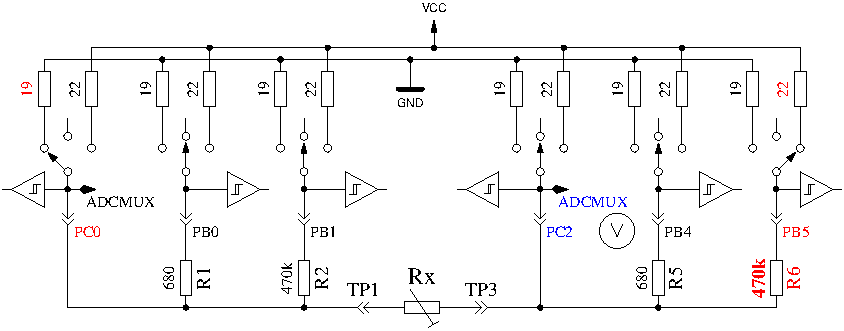
\includegraphics[width=.8\textwidth]{../FIG/ResistormessH1.pdf}
\caption{Měření typu 3 s \(470k\Omega\) }
\label{fig:RH1mes}
\end{figure}

\begin{figure}[H]
 \centering
 \includegraphics[width=.8\textwidth]{../FIG/ResistormessH2.pdf}
 \caption{Měření typu 4 s \(470k\Omega\) }
\label{fig:RH2mes}
\end{figure}

\begin{figure}[H]
\centering
 \includegraphics[width=.8\textwidth]{../GNU/RHvCZ.pdf}
\caption{Napětí při měření typu 3 a typu 4 s \(470k\Omega\) }
\label{fig:RHv}
\end{figure}

\subsection{Výsledky měření odporů}
Obrázek~\ref{fig:mega8res}  ukazuje relativní chybu měření odporu se třemi různými ATmega8.
Kromě toho jsou výsledky měření některých odporů s původním softwarem Markuse F. zobrazeny jako ,,Mega8orig''.
Výsledky měření stejných odporů se třemi ATmega8A a třemi ATmega8L jsou uvedeny
na obrázcích\ref{fig:mega8Ares} a \ref{fig:mega8Lres}.
Obrázek~\ref{fig:mega168res} ukazuje stejné měření pomocí ATmega168.
,,Mega168'' jsou výsledky bez možnosti AUTOSCALE\_ADC, ,,Mega168as'' s touto možností.
S ATmega168 se zdá být možné získat měření odporu v rozsahu od \(20\Omega\) bis
\(20M\Omega\) s chybou měření menší než  \(\pm1\%\).
Pro měření pod \(100\Omega\)je třeba vzít v úvahu, že každá zkušební šňůra má také nějakou hodnotu odporu.
Je lepší připojit měřěný objekt přímo ke svorkám.
Pokud to není možné, je třeba od výsledku měření odečítat odpor zkratovaných zkušebních šnůr.
Například. Tester zobrazí hodnotu \(30,6\Omega\). Pokud má přesný odpor vytištěnou hodnotu \(30\Omega\)
a zkratované zkušební kabely mají hodnotu  \(0,5\Omega\), pak je skutečná hodnota odporu \(30,1\Omega\).
Pod hodnotou odporu \(10\Omega\), činí krok rozlišení \(0,1\Omega\) již chybu více než \(1\%\)!

\begin{figure}[H]
\centering
 \includegraphics[width=.8\textwidth]{../GNU/Mega8resCZ.pdf}
\caption{Relativní chyba pro měření odporu s ATmega8}
\label{fig:mega8res}
\end{figure}

\begin{figure}[H]
  \begin{subfigure}[b]{.5\textwidth}
    \centering
    \includegraphics[width=1.\textwidth]{../GNU/Mega8AresCZ.pdf}
    \caption{Se třemi ATmega8A}
    \label{fig:mega8Ares}
  \end{subfigure}
  ~
  \begin{subfigure}[b]{.5\textwidth}
    \centering
    \includegraphics[width=1.\textwidth]{../GNU/Mega8LresCZ.pdf}
    \caption{Se třemi ATmega8L}
    \label{fig:mega8Lres}
  \end{subfigure}
\caption{Relativní chyba při měření odporů}
\end{figure}

\begin{figure}[H]
\centering
\includegraphics[width=.8\textwidth]{../GNU/Mega168resCZ.pdf}
\caption{Relativní chyba při měření odporů s ATmega168}
\label{fig:mega168res}
\end{figure}

Diagram \ref{fig:m168res_all} ukazuje chyby měření tří procesorů ATmega168 před kalibrací jako body,
po kterých kalibrace jako přímka.
Tomu odpovídá  měření chyb u tří ATmega168A na obr. \ref{fig:m168ares_all} a tří ATmega328P
zobrazených na obrázku \ref{fig:m168pres_all}.
Chyby měření ATmega328 jsou zobrazeny na obrázcích \ref{fig:m328res_all} a \ref{fig:m328pres_all}.
Po automatické kalibraci zůstává chyba měření v rozsahu odporu s jednou výjimkou (ATmega328P-13, \(22k\Omega\)), 
\(10\Omega~-~20M\Omega\) v rozsahu \(\pm1\%\).
Před kalibrací dosahovaly chyby měření v některých procesorech až \(\pm~3\%\).
Chyba je způsobena přepnutím ADC reference AUTOSCALE\_ADC.
Přímým porovnáním napětí kondenzátoru pod \(1V\), jednou s VCC odkazem a opět s měřením interní referencí , může být chyba kompenzována.
V tomto případě je napětí měřeno stejným kanálem multiplexeru a referenční pásmo je na AREF kolíku
zapnuté.
Přímé měření (Bandgap-reference) přímou volbou vstupu multiplexeru bohužel vede k tomuto ofsetu,
který lze ručně odstranit pomocí volby REF\_R\_KORR nebo automaticky s volbou AUTO\_CAL auto-testu.
V režimu AUTO\_CAL-Modus je REF\_R\_KORR další ofset k automaticky zjištěnému rozdílu napětí.

\begin{figure}[H]
  \begin{subfigure}[b]{.5\textwidth}
    \centering
    \includegraphics[width=1.\textwidth]{../GNU/m168res_allCZ.pdf}
    \caption{Se třemi ATmega168}
    \label{fig:m168res_all}
  \end{subfigure}
  ~
  \begin{subfigure}[b]{.5\textwidth}
    \centering
    \includegraphics[width=1.\textwidth]{../GNU/m168ares_allCZ.pdf}
    \caption{Se třemi ATmega168A}
    \label{fig:m168ares_all}
  \end{subfigure}
\caption{Relativní chyba při měření odporů}
\end{figure}

\begin{figure}[H]
\centering
\includegraphics[width=.8\textwidth]{../GNU/m168pres_allCZ.pdf}
\caption{Relativní chyba při měření odporů se třemi ATmega168P }
\label{fig:m168pres_all}
\end{figure}

\begin{figure}[H]
  \begin{subfigure}[b]{.5\textwidth}
    \centering
    \includegraphics[width=1.\textwidth]{../GNU/m328res_allCZ.pdf}
    \caption{Se třemi ATmega328}
    \label{fig:m328res_all}
  \end{subfigure}
  ~
  \begin{subfigure}[b]{.5\textwidth}
    \centering
    \includegraphics[width=1.\textwidth]{../GNU/m328pres_allCZ.pdf}
    \caption{Se třemi ATmega328P}
    \label{fig:m328pres_all}
  \end{subfigure}
\caption{Relativní chyba při měření odporů}
\end{figure}


 \section{Measurement of Capacitors}
The measurement of capacitor values are done as separate task by measurement of load time
after all other measurements. 
The original software of Markus F. did this with a program loop, which reads the corresponding digital input
pin until a switch occured and count the loop cycles.
This has the handicap, that the resolution of time measurement is limited by the
time consumption of one loop cycle.
This usually was done in all six combinations for all three probe pins. 
The actual software uses two different ways to get the load time in only
three combinations for the three probe pins. The positive side is now always the
higher probe number. Only if capacity is measured parallel with a diode, the
polarity can be in the other order.

\subsection{Discharging of Capacitors}
You should always discharge the capacitor before connecting it to the tester.
The tester additionally discharge the capacitor before any measurement.
If the voltage is below \(1300mV\), the capacitor is shortened by the output pins of the connected ADC port (Port C).
I~believe that this is legal because every output port has a built in resistance of about \(20\Omega\).
The data sheet Figure 149 (page 258) \cite{ATmega8} shows voltage drop of output pins up to \(2V\).
Of course I can not guaranty, that no damage can occur. 
I~have tested the function with big capacitors of more than \(15mF\) many times and I~have never noticed any problem.
The current should be below the specified limit of \(40mA\) and is reduced fast by discharging.
Off course damage can occur if you do not discharge a (high voltage) capacitor before connecting it to your tester.

\subsection{Measurement of big Capacitors}
\label{sec:bigcap}
One side of the capacitor is connected to GND. The other side of the capacitor is connected with the
\(680\Omega\) resistor to VCC for a period of 10ms. Afterwards this probe pin is switched to Input (High Impedance).
After this \(10ms\) current pulse the voltage of the capacitor is measured without any current. If the voltage has not
reached a minimal value of \(300mV\), the load pulse is repeated up to 499 times.
If after 127 pulses a minimum voltage of \(75mV\) is not reached (about 2s), further load is stopped, because never
the \(300mV\) can be reached with the remaining load pulses.
Figure~\ref{fig:bigcap} shows the three phases of measuring the capacity value of a capacitor.
The value of the capacity is then computed with the count of load pulses and the reached load voltage from a table.
The table contains  the factors to get the capacity in nF units from load time and the reached voltage
with a spacing of \(25mV\).
Interim value of voltage will be interpolated.

\begin{figure}[H]
\centering
 \begin{overpic}[width=.93\textwidth]{../FIG/Bigcap.pdf}
  \color{black}
  \put(25,97){\makebox(0,0)[cb]{Quick Discharge of capacitor}}
  \put(25,61){\makebox(0,0)[cb]{10ms Charge Phase of capacitor}}
  \put(25,26){\makebox(0,0)[cb]{Voltage Measurement Phase of capacitor}}
 \end{overpic}
\caption{discharge a capacitor and load with \(10ms\) load pulses until voltage reach a value of \(300mV\)}
\label{fig:bigcap}
\end{figure}
As a result of the low load voltage, the measurement is much faster than the initial software version,
 because this advantage works also on discharging. So bigger capacitors can be measured.
Furthermore a diode, which is parallel connected to the capacitor don´t disturb the measurement in most cases,
because the flux voltage of most diodes is not reached.
Beginning with software version 1.12k a trickery is used to measure the residual voltage of a capacitor
before the capacity measurement. 
Depending on the previous history of the capacitor the residual voltage can be positive or negative.
Negative voltages can not be measured with the ADC. For that reason the voltage of the negative test pin
is raised with the \(680\Omega\) resistor to about \(132mV\) as shown in figure~\ref{fig:CapResidV}.
With the difference of the voltages measured at both sides of the capacitor the residual voltage can
be build with any polarity. The voltage of the positive test pin remains positive in any case, even if
the capacitor have a negative residual voltage of some mV.

\begin{figure}[H]
\centering
\includegraphics[width=.8\textwidth]{../FIG/Cap_residV.pdf}
\caption{Measurement of the residual voltage of a capacitor before loading}
\label{fig:CapResidV}
\end{figure}

Figure~\ref{pic:c229} shows the charge and discharge for a \(229\mu F\) capacitor.
The flat top of diagram from load end to discharge begin is caused by the measuring and computing time of the ATmega.
Figure~\ref{pic:c5mF} shows the same measurement for a~\(5mF\) capacitor,
notice how the time for measurement is grown to about 1.5 seconds inclusive the discharge. 
The last example shows the capacity measuring of a~\(15mF\) capacitor in Figure~\ref{pic:c15mF}

\begin{figure}[H]
  \begin{subfigure}[b]{.5\textwidth}
    \centering
    \includegraphics[width=1.\textwidth]{../PNG/charge_229uF.png}
    \caption{\(229\mu F\) Capacitor}
    \label{pic:c229}
  \end{subfigure}
  ~
  \begin{subfigure}[b]{.5\textwidth}
    \centering
    \includegraphics[width=1.\textwidth]{../PNG/charge_5mF.png}
    \caption{\(5mF\) Capacitor}
    \label{pic:c5mF}
  \end{subfigure}
  \caption{Charge and discharge of big Capacitors for measuring}
\end{figure}

\begin{figure}[H]
  \centering
    \includegraphics[width=.8\textwidth]{../PNG/charge_15mF.png}
  \caption{Charge and discharge of a \(15mF\) Capacitor for measuring}
  \label{pic:c15mF}
\end{figure}

After this capacity measurement the self-discharge of the capacitor will be checked by
waiting a proportional period the loading has taken and reading the load voltage again.
The measured capacity value is corrected due to this voltage drop.
A test with a parallel connection of a \(68\mu F\) capacitor and a \(2.2k\Omega\) resistor shows
the effectivity of this method.
The measured capacity value without the resistor is \(66.5\mu F\),
with the parallel \(2.2k\Omega\) resistor results to a capacity value of \(66.3\mu F\).
For comparison here are the results measured with a Peaktech 3315 multimeter:
Without the resistor a capacity value of \(68.2\mu F\) is measured, with the
parallel \(2.2k\Omega\) resistor a value of \(192\mu F\) is measured with the multimeter.


\subsection{Measurement of small Capacitors}
If the first \(10ms\) load pulse has overloaded the capacitor, another technique of measurement is used.
The ATmega processor has a build in 16-Bit counter, which can operate at the full clock rate (\(1MHz\) or \(8MHz\)).
This counter has also the feature to save his counter value by a external event.
This event can be built by the output of the comparator. 
The comparator can operate with any ADC input pin and the band gap reference.
Figure~\ref{fig:comparat} shows a simplified diagram of the measurement situation.
So I discharge the capacitor, prepare the comparator to the proper pin input, start the counter at 0 and
start immediately the charging of the capacitor with one side connected to GND and the other side connected with
the \(470k\Omega\) resistor to VCC.
Now I check within a program loop, if the counter flags signals a overflow event or a input capture (external) event.
I count the overflow events until I detect the input capture event.
In this case I stop the counter and check if I must count a additional overflow,
because the counter can't be stopped by the input capture event.


The input capture counter and the overflow counter built together the total time,
from which we can get the capacity with a factor.
The actual software can use a table with the theoretical  dependency of the load time in respect to the comparator voltage.
The table is spaced in \(50mV\) steps and will be interpolated according to the actual reference voltage. 
This table will only be acticated with the Makefile option WITH\_AUTO\_REF.
From the build capacity value I subtract a predefined experimental find out constant or a value found by the last selftest
with AUTO\_CAL option to eliminate the zero offset. 
The zero offset may vary with printed board type, the used test equipment or processor.
The selftest with AUTO\_CAL option will find out your zero offset automatically.

I noticed that the reference voltage is permanently somewhat to low,
 so that you can choose an offset with the Makefile option REF\_C\_KORR.
After calibration with the AUTO\_CAL option , the REF\_C\_KORR will only be a offset to the measured difference voltage
between loaded capacitor and internal reference.
The measured reference voltage will then be corrected (added) by your value (mV units).
If option WITH\_AUTO\_REF is not used, the reference voltages of ATmega8, ATmega168 and ATmega328
are applied as noted in the data sheets~\cite{ATmega8}~\cite{ATmega168}. 
A sample measurement of this type is shown in figure~\ref{pic:c22uF}.
The measurement time for the \(22\mu F\) capacitor is above \(2.6s\) because the \(470k\Omega\) is
used for charging. But discharging is in this case much faster than charging.

\begin{figure}[H]
\centering
\includegraphics[width=.8\textwidth]{../FIG/Comparat.pdf}
\caption{measurement little capacity values with comparator}
\label{fig:comparat}
\end{figure}

\begin{figure}[H]
  \centering
    \includegraphics[width=.8\textwidth]{../PNG/charge_22uF.png}
  \caption{Charge and discharge of a \(22\mu F\) Capacitor for measuring}
  \label{pic:c22uF}
\end{figure}


In principle this technique of measurement can also be done with the \(680\Omega\) resistor, but 
because the ADC can't be used if the comparator is working, I have no chance to monitor the
load voltage until the comparator is stopped. If a undetected diode is parallel connected with
the capacitor, the load current of the capacitor can be absorbed by the diode (threshold voltage) and
the band-gap voltage will never be reached.
The method taken in actual software for big capacitors in section~\ref{sec:bigcap}
avoids this conceptual bug.

\subsection{Measurement of very small capacity values with the sampling technique}
The radio amateur Pieter-Tjerk (PA3FWM) has integrated the measurement capability for very small
capacity values (\textless~100pF) with the sampling technique.
The conversion period of the ADC is in fact too long for sampling a fast signal directly.
But the voltage of the input signal is hold at a specified time of the conversion cycle,
the Sample and Hold (SH) time.
The ADC need 13 clock cycles for a total conversion and the ADC clock is build by dividing the
processor clock by 128 or 64.
The input voltage is fixed at exactly ADC clock number 1.5 for continuous cycles.
If the input signal can be generated again and again, we can shift the sample time of the ADC from
one to the next signal repetition, so that we get a sample sequence of the fast signal.
A normal ADC cycle takes 13x64 = 832 clock cycles with a 8~MHz processor clock.
If we repeat the input signal with a 831 clock cycle, a uninterrupted ADC (free rum mode) would
sample the signal one processor clock tick later for every following signal repetition.
We must make sure with this method, that the first ADC sampling of the signal is done at
the requested starting time. The time of the following ADC samples would be shifted by one processor clock
tic later for every next signal repetition.
If the signal can be repeated exactly, the combined signal of many periods is the same, 
which would be sampled and converted directly with a ADC running with the processor clock (8~MHz).
Figure~\ref{fig:sampling} shows the principle of sampling a ten times repeated signal
to get 10 samples (SH0 - SH9).
In reality the relativ time shift of successive samples is much smaller than shown here.

\begin{figure}[H]
\centering
\includegraphics[width=1.\textwidth]{../FIG/sampling.pdf}
\caption{Scanning of a voltage curve with the sampling technique}
\label{fig:sampling}
\end{figure}

One problem to fix the exactly time of the first sample is given by a continuous running clock precaler.
Only a trigger of a external signal can reset the ADC clock divider.
The clock divider would resume with dividing, if the ADC is started by program intruction.
Only a program written in assembly language can specify the exactly points in time for
this sampling technique. Every clock tick is important for building the program loops.

By analysing the voltage characteristic of charging a small capacitor you can see, that the time constant
is not continuous during the sampling period. This was shown by Pieter-Tjerk at a presentation at
the \inquotes{60. UKW-Tagung in Weinheim}. The internal capacitor of about 10~pF, which hold the input voltage
for the conversion, is uncoupled at the SH time and connected again two ADC clock cycles later. 
Additionally there is a little jamming in the data just a half clock before the reconnection,
which is probably caused by the switch of the multiplexor.
Both disturbancies are respected with the data processing in the software.
The sampling software can handle up to 255 samples. The software can also build the mean value of
up to 32 charge sequencies. By building the mean value the effect of noise trouble will be less.
The sampling software can monitor and process both, the charge or the discharge of a capacitor.
Because both charge directions are used to measure the capacity value of a diode in reverse direction,
the calibration task measure the zero capacity value in both charge direction for all pin combinations.
By measuring the capacity value of a diode in both charge directions, the difference between both
values can be shown.
With the charge direction a capacity value is measured near the voltage 0 and with
the discharge direction the capacity is measured near a voltage of 5V.
With normal capacitors there is no difference in the capacity values with this little voltage difference detectable.
Therefore only the charge direction is used for measuring little capacities (\textless 100pF).

Pieter-Tjerk has optimized his function for a 16~MHz operation.
In this configuration you will get a resolution of 0.01~pF.
For the 8~MHz operation the ADC will run at the half speed for getting the above-mentiored disturbances
at the same data points compared to the 16-MHz operation.
The loss of resolution with the 8~MHz operation will be irrelevant for most users and the
additional testing time with the slower ADC in this mode is tolerable too.



\subsection{Measurement of the Equivalent Series Resistance ESR}
The series resistance ESR \cite{ESR} is a good indicator for the aging of electrolytical capacitors for example.
The figure ~\ref{fig:Cap_equiv} shows a equivalent circuit of a capacitor.
The resistor \(Rp\) represents the leakage resistance of the capacitor, \(ESL\) the equivalent series inductivity and
the resistance \(ESR\) represents the equivalent series resistance.

\begin{figure}[H]
  \centering
    \includegraphics[width=.3\textwidth]{../FIG/Cap_equiv.pdf}
  \caption{Equivalent circuit of a capacitor}
  \label{fig:Cap_equiv}
\end{figure}

Usually the data sheets publish ESR values, which are measured with a frequency of 100 kHz and a temperture 
of 20\textdegree C .
The figures~\ref{fig:Cap_FC_data} and \ref{fig:Cap_FR_data} shows the ESR values of the Panasonic series FC and 
the \inquotes{low ESR} series FR.
Both series are able to operate up to a temperature of 105\textdegree C.
The figure~\ref{fig:Cap_FC_FR_data} shows the data of both series with a allowable working stress of \(25V\).
If the series have different types with the same capacity and voltage range, the one with the lowest ESR is
taken for the diagram.
The values of capacity and ESR of electrolytic capacitors change significant with there operating temperature.

\begin{figure}[H]
  \centering
    \includegraphics[width=.8\textwidth]{../GNU/Cap_FC_dataEN.pdf}
  \caption{ESR data from the Panasonic data sheet of the series FC}
  \label{fig:Cap_FC_data}
\end{figure}

\begin{figure}[H]
  \centering
    \includegraphics[width=.8\textwidth]{../GNU/Cap_FR_dataEN.pdf}
  \caption{ESR data from the Panasonic data sheet of the series FR}
  \label{fig:Cap_FR_data}
\end{figure}

\begin{figure}[H]
  \centering
    \includegraphics[width=.8\textwidth]{../GNU/Cap_FC_FR_dataEN.pdf}
  \caption{Comparison of the ESR data from series FC with series FR}
  \label{fig:Cap_FC_FR_data}
\end{figure}

There is no simple way to measure the ESR with a frequency of 100 kHz with the ATmega hardware,
because neither the ADC can sample a so high input frequency, nor the existing circuit can support
with a \(100kHz\) signal.
At next there will be introduced two method's for the measurement of the ESR, which both manage on 
the existing circuit.
Both method's use a rectangular signal for the measurement, so that the results will never be
the same with the values measured with sinusoidal signal.
With the first method the measured values are close to those values, which are measured with a
\(1kHz\) signal. 
But the second method has the advantage, that the zero value can be determined with shorted test pads and
that additionally the measured ESR is more close to the value measured with \(10kHz\) signal.
Currently I have no idea for a measurement method, which can produce a ESR value close to the
value of a \(100kHz\) measurement.

The following table~\ref{tab:capESR} should show the dependency of the ESR results from measurement frequency.
All capacitors without the \(47\mu F\) capacitor are from the same FC series of manufactor Panasonic.
The reference values are measured with a Peaktech 2170 LCR meter.
All results of the TransistorTester are measured with the method 2 of subchapter~\ref{sec:ESR2} .
Capacitors with big capacity values are difficult to measure with higher frequencies like \(100kHz\) because
the inductance ESL make trouble.

\begin{table}[H]
  \begin{center}
    \begin{tabular}{| l | c | c | c | c | c |}
   \hline
            & Data sheet & PeakTech  & Peaktech & PeakTech & Transistor- \\
Capacitor   & 100~kHz    & 100~kHz   & 10~kHz   & 1~kHz    & tester  \\
    \hline
    \hline
1uF / 50V    & 2.4       & 1.27      & 1.75     & 4.31     &  2.1 \\
    \hline
2.2uF / 50V  & 1.8       & 1.07      & 1.34     & 2.76     &  1.6 \\
    \hline
4.7uF / 50V  & 1.3       & 1.19      & 1.40     & 2.37     &  1.5 \\
    \hline
4.7uF / 50V  & 1.3       & 1.19      & 1.40     & 2.37     &  1.5 \\
    \hline
10uF / 50V   & 1.3       & 1.26      & 1.45     & 2.05     &  1.5 \\
    \hline
22uF / 10V   & 2.0       & 1.52      & 1.76     & 2.24     &  1.9 \\
    \hline
47uF / 63V   & ?         & 0.46      & 0.50     & 0.63     &  0.52 \\
    \hline
    \end{tabular}
  \end{center}
  \caption{ESR values of different electrolytical capacitors}
  \label{tab:capESR} 
\end{table}


\subsection{Measurement of the Equivalent Series Resistance ESR, first way}
If the measured capacitor has a capacity of more than \(0.45\mu F\), the tester will try to measure
the series resistance too.
For a capacity of more than \(3.6\mu F\) the normal clock rate of \(125kHz\) for the Analog-Digital converter is used.
For lower capacities the higher clock rate of \(500kHz\) is used to accelerate the measurement.
The accuracy of the ADC results will be more worth by the higher clock rate, but this could be accepted by the
higher ESR values of capacitors with lower capacity.
Otherwise the measurement of ESR with this method is not possible for a capacity of less than \(1.8\mu F\) at the normal
clock rate of \(125kHz\).

Strictly speaking the ESR of a capacitor depends on the operating frequency and temperature.
Usually the value measured with sine wave-form signal of \(100kHz\) is denoted in the data sheets.
This measurement can not be done with the ATmega without external equipment.
With the subsequent written method the measurement frequency with the standard ADC clock rate will be below 640 Hz
with nearly rectangular signal. With \(500kHz\) ADC clock rate the measurement frequency will be 2400 Hz.
To get the value of the equivalent series resistance,
the voltage of both connections will be measured during loading in one direction with the ADC internal reference 
voltage (\(1.1V\)).
After the measurement the load current will be switched off and the voltage of the capacitor is measured
again without the current.
If this voltage is below \(3mV\), the sequence of measurement is repeated.
The figure~\ref{fig:Cap_esr} shows the corresponding circuits.

\begin{figure}[H]
 \centering
  \begin{overpic}[width=.83\textwidth]{../FIG/Cap_esr.pdf}
   \color{black}
   \put(28,85){\makebox(0,0)[cb]{Voltage measurement with charge current}}
   \put(28,40){\makebox(0,0)[cb]{Voltage measurement without current}}
  \end{overpic}
 \caption{Circuit of the ESR measurements of a capacitor}
 \label{fig:Cap_esr}
\end{figure}

The difference of capacitor voltages with and without current is proportional to the internal resistance of the capacitor. 
The expected voltage of this difference is so low, that one measurement can not result to a feasible result.
Therefore after this the current will be switched to the opposite direction and the same measurement will be repeated.
The whole measurement sequence will be done 128 times and the results of the voltage measurements will be added.
So we have three sums of voltages, the voltage \(Ulp\) at the low side of the capacitor with current, the voltage \(Uhp\) at
the high side of the capacitor with current and the voltage \(Uc\) of the high side of the capacitor without current.
The sum of voltages at the low side of the capacitor represents the potential drop with the mean load current at
the port output resistance \(Rport\). 
The voltage difference  of the high side and the low side of the capacitor represents the voltage of the capacitor with
load current \(Udiff = Uhp - Ulp\).
The difference \(Uesr = Udiff - Uc\) should represent the voltage drop at the internal resistance of the capacitor with
mean load current.
We will get the resistance value with the relation of this voltage \(Uesr\) to the voltage \(Ulp\), scaled with the
known resistance value of the port output \(Rport\).
The scale factor is selected to get a resistance resolution of \(0.01\Omega\):  \(Resr = \frac{Uesr \cdot 10 \cdot Rport}{Ulp}\)
The figure~\ref{pic:esr4} shows a part of the voltage curve of a \(4.2\mu F\) capacitor during the ESR measurement.
To explain the influence of the ESR, a series \(6.8\Omega\) resistor is added to the capacitor.
The little voltage break after loading the capacitor is interpreted by software to get the ESR.
The greater voltage drop of the measurement to GND potential is caused by the port output resistance of about \(20\Omega\).
For this measurement a total ESR of \(7.5\Omega\) is reported by the tester, without the series \(6.8\Omega\) resistor a ESR of \(0.56\Omega\) is found.
The figure~\ref{pic:esr2} shows the same measurement with higher measurement frequency of a \(2.2\mu F\) electrolytical capacitor
with a ESR of \(6.5\Omega\).


\begin{figure}[H]
  \begin{subfigure}[b]{.5\textwidth}
    \centering
    \includegraphics[width=1.\textwidth]{../PNG/ESR_4uF.png}
    \caption{measured one pin to GND}
  \end{subfigure}
  ~
  \begin{subfigure}[b]{.5\textwidth}
    \centering
    \includegraphics[width=1.\textwidth]{../PNG/ESR4uF6R8.png}
    \caption{measured pin to pin}
  \end{subfigure}
  \caption{Voltage curve of a \(4.2\mu F\) capacitor during the ESR measurement}
  \label{pic:esr4}
\end{figure}


\begin{figure}[H]
  \begin{subfigure}[b]{.5\textwidth}
    \centering
    \includegraphics[width=1.\textwidth]{../PNG/ESR_2uF_pin2GND.png}
    \caption{measured one pin to GND}
  \end{subfigure}
  ~ 
  \begin{subfigure}[b]{.5\textwidth}
    \centering
    \includegraphics[width=1.\textwidth]{../PNG/ESR_2uF_pin2pin.png}
    \caption{measured pin to pin}
  \end{subfigure}
  \caption{Voltage curve of a \(2.2\mu F\) capacitor during the ESR measurement}
  \label{pic:esr2}
\end{figure}



The accuracy of the ESR measurement is not very high by different reasons:
\begin{enumerate}
\item The voltage measurement at both pins of the capacitor can not be done at the same time, the only way is to do it in sequence.
In the interim time between both measurements the load current has changed due to the charge of capacitor.
The program tries to compensate this fact with a capacity dependent correction of the low side voltage.
\item The ADC takes the measurement voltage after 1.5 clock ticks after the start of conversion.
The conversion beginns with the rising edge of the ADC-clock, if the start bit is set.
If the charge current will be switched off to early, the ADC takes the wrong voltage for the measurement with current.
If the charge current will be switched off to late, the capacitor will take more electric charge, than that of the
corresponding measurement with load current. This will cause a too high voltage of the measurement without current.
But it is difficult to switch off the current at the right time by software. 
\item The port output resistance is used as a reference value by this measurement method, but this resistance value is
not exacly known too.
\item The resolution of the ADC is not sufficient to get a resolution of resistance of \(0.01\Omega\).
To get the best avaiable resolution of ADC, the internal reference (\(1.1V\)) is used for all measurements.
The resolution deficit will be attenuated by accumulating a big number of single measurements too.
\item The switching of ports can not be exactly synchronized to the ADC clock with polling of conversion done.
\end{enumerate}

Anyway the results seems to be practical, as shown with the following figure~\ref{fig:Cesr}.
The ESR values of the same part measured with the Transistortester vary more than the values measured with the LCR meter.
The ESR values from the LCR meter are measured with a frequency of \(1kHz\) or are interpolated for little capacities to
\(2.4kHz\).
You must respect the quality of all connection parts. The used cable connections can cause a higher measured resistance value.
The plug connectors can also result a higher resistance value.
The LCR meter has the advantage of the used Kelvin terminals.
Only one capacitor with a capacity below \(1\mu F\) was a \(500nF\) ceramic type, all others were
plastic film capacitors.
The only electrolytical capacitor of the test series below \(9\mu F\) was a \(2.2\mu F\) capacitor.

\begin{figure}[H]
\centering
\includegraphics[width=.93\textwidth]{../GNU/CesrEN.pdf}
\caption{ESR measurement results of 15 different ATmega}
\label{fig:Cesr}
\end{figure}


\subsection{Measurement of the Equivalent Series Resistance ESR, second way}
\label{sec:ESR2}
From beginning with software version 1.07k the ESR measurement way is changed to a new measurement method.
The different measurement steps are shown in figure~\ref{fig:Cap_esr2}. The difference to the previous way is that
the period of current flow through the capacitor is essential shorter.
The capacitor is preloaded with a half pulse to the negative direction and is than loaded in a cyclic way in both
direction.
The timing of the load pulse is so selected, that the middle of the load puls at sample 4 and 8 is
pointed to the sample and hold time of the ADC (2.5 clock tics after start of ADC). 
A complete measurement cycle is shown in figure~\ref{fig:Cap_esr2_timing}.
The sums of 255 measurement cycle results is used for getting a result with adequate resolution. 
A continuing charge of the capacitor in any direction is avoided by the same charge and discharge pulse length
and the same circuit.
By measuring the reference voltage the capacitor remains currentless. By that this measurement are not time critital.
It is only assumed, that the capacitor hold the voltage until the next charge or discharge pulse begins.

\begin{figure}[H]
  \centering
    \includegraphics[width=1.\textwidth]{../FIG/Cap_esr2_timing.pdf}
  \caption{Timing of a measurement cycle for the new ESR-measurement way}
  \label{fig:Cap_esr2_timing}
\end{figure}

\begin{figure}[H]
 \centering
  \begin{overpic}[width=.83\textwidth]{../FIG/Cap_esr2.pdf}
   \color{black}
   \put(20,98){\makebox(0,0)[cb]{Forward reference measurement}}
   \put(20,72){\makebox(0,0)[cb]{Forward voltage measurement with probe current}}
   \put(20,47){\makebox(0,0)[cb]{Reverse reference measurement}}
   \put(20,21){\makebox(0,0)[cb]{Reverse voltage measurement with probe current}}
  \end{overpic}
 \caption{More simple ESR measurement of a capacitor}
 \label{fig:Cap_esr2}
\end{figure}


Due to the shorter load puls not only the ESR of capacitors with lower capacity can be measured, but this
way of measurement can also be used for the measurement of resistors with little resistance, if they don't
have a detectable inductance. By doing that, a resolution of \(0.01\Omega\) for this resistors can be achieved.
Also the zero resistance can be detected by the calibration part of the selftest for all three test pin combination.
You should keep in mind, that stable plug sockets or clamping connectors are essential for stable results.
The measurement periode is about \(900\mu s\), which results to a frequency of about \(1.1kHz\).
Because the load pulse is very short, the measurement result is comparable to measurements with \(10kHz\).
A measurement example with a \(10\mu F\) foil capacitor, once measured alone and once measures with a \(2.7\Omega\)
series resistor is shown in figure~\ref{pic:NewEsr10}.
You can see the effect of the additional resistance by comparing both diagrams.
You can see also, why the ADC measurement (SH) should point to the middle of the load pulse.
With big capacity values the load current is nearly stable during the total pulse length,
so you will get the middle voltage at the middle time of the load pulse. 
With lower capacity values you will get a significant difference, which can be compensated by the
known capacity value.

\begin{figure}[H]
  \begin{subfigure}[b]{.5\textwidth}
    \centering
    \includegraphics[width=1.\textwidth]{../PNG/NewEsr10uF0R0.png}
    \caption{without series resistance}
  \end{subfigure}
  ~
  \begin{subfigure}[b]{.5\textwidth}
    \centering
    \includegraphics[width=1.\textwidth]{../PNG/NewEsr10uF2R7.png}
    \caption{with \(2.7\Omega\) series resistance}
  \end{subfigure}
  \caption{Voltage curve of a \(10\mu F\) capacitor during new ESR measurement}
  \label{pic:NewEsr10}
\end{figure}


By using the \(27\mu s\) long charge pulses the ESR of capacitors above \(180nF\) can be determined.
For measuring of capacitors with lower capacity the current pulse is shortened to \(8\mu s\) for version 1.11k.
The figures~\ref{pic:NewEsr2} show the voltage curve of a \(2.2\mu F\) capacitor without and with
a \(2.7\Omega\) series resistor.

\begin{figure}[H]
  \begin{subfigure}[b]{.5\textwidth}
    \centering
    \includegraphics[width=1.\textwidth]{../PNG/NewEsr2u2F0R0.png}
    \caption{without series resistance}
  \end{subfigure}
  ~
  \begin{subfigure}[b]{.5\textwidth}
    \centering
    \includegraphics[width=1.\textwidth]{../PNG/NewEsr2u2F2R7.png}
    \caption{with \(2.7\Omega\) series resistance}
  \end{subfigure}
  \caption{Voltage curve of a \(2.2\mu F\) capacitor during new ESR~measurement with \(8\mu s\) charge pulses}
  \label{pic:NewEsr2}
\end{figure}

Because you can not see the sample and hold time of the ADC in the figures~\ref{pic:NewEsr2},  the voltage curve is shown zoomed
in figures~\ref{pic:NewEsr2zoom}. The sample and hold time is approximately in the middle of the screen picture.

\begin{figure}[H]
  \begin{subfigure}[b]{.5\textwidth}
    \centering
    \includegraphics[width=1.\textwidth]{../PNG/NewEsr2u2F0R0zoom.png}
    \caption{without series resistance}
  \end{subfigure}
  ~
  \begin{subfigure}[b]{.5\textwidth}
    \centering
    \includegraphics[width=1.\textwidth]{../PNG/NewEsr2u2F2R7zoom.png}
    \caption{with \(2.7\Omega\) series resistance}
  \end{subfigure}
  \caption{Zoomed voltage curve of a \(2.2\mu F\) capacitor during new ESR~measurement with \(8\mu s\) charge pulses}
  \label{pic:NewEsr2zoom}
\end{figure}
 

The measurement results of the new ESR measurement method is shown in figure~\ref{fig:Cesr2}.
The ESR values are different from the results shown for the previous mesurement procedure in figure~\ref{fig:Cesr} because 
the ESR is frequency dependence of the ESR.
The reference values are determined with a LCR meter at a measurement frequency of \(10kHz \).

\begin{figure}[H]
\centering
\includegraphics[width=.93\textwidth]{../GNU/Cesr2EN.pdf}
\caption{ESR results with 15 different ATmega, method 2}
\label{fig:Cesr2}
\end{figure}

A measurement series with different sized electrolytic capacitors are shown in figure~\ref{fig:ElcoESR}.
The results of a PeakTech 3315 LCR meter of measurements with different frequencies and the results of the
TransistorTester are shown together. The resistance is illustrated with logarithmic scale in this diagram. 
In all cases the results of the TransistorTester is near by the results of
the \(10kHz\) measurements of the LCR meter.
Only the \(500\mu F/3V\) capacitor is a older exemplar, all others capacitors are as good as new.

\begin{figure}[H]
\centering
\includegraphics[width=1.\textwidth]{../GNU/Elco_esrEN.pdf}
\caption{Results of the ESR measurements of different electrolytic capacitors}
\label{fig:ElcoESR}
\end{figure}


Because the new measurement method can be taken for measuring of resistors with low values, the
measurement errors of some resistors below \(10\Omega\) with three example of each ATmega type will be shown in
figure~\ref{fig:res_esr}. 

\begin{figure}[H]
\centering
\includegraphics[width=1.\textwidth]{../GNU/res_esrEN.pdf}
\caption{Measurement errors of resistors with the ESR method}
\label{fig:res_esr}
\end{figure}

With software version 1.12k the load pulse length for the capacitors is reduced to \(2\mu s\) to accomplish ESR measurements
of capacitors with lower capacity values. Now a ESR-value can be measured for capacity values above \(20nF\).
But the measurement error will grow for lower capacity values. The reason for that is the decrease of the time constant of the
RC-circuit, which will be only about \(14.4\mu s\) for a capacity value of \(20nF\).
This will result to a fast change of the capacitor voltage during the \(2\mu s\) current pulses.
The software can select the sampling instance of the ADC only to the time of any processor clock.
But the input filter of the ADC has a time constant of about \(0.24\mu s\), which can vary from exemplar to examplar of the ATmega.
This change of the ADC input filter time constant can not be respected with the software.
For this purpose the ADC sample time must be selectable to a fraction of the processor clock period.
With greater capacity values of the measurement object the time constant will grow and the voltage change during the
load pulse will decrease. For this reason the variation of the ADC input filter time constant  has
lower effect with greater capacity values.
The examples in figures~\ref{pic:Cesr_22n} show the results for some capacitors with 10 different tester examples. The picture at the left side
shows the ESR results of some capacitors with higher ESR values. The result is rather simular compared with the results
of the Peaktech 2170 LCR meter at \(10kHz\) and at \(100kHz\).
At the right picture you can see the measurement results of some high quality capacitors with low ESR values.
Altough you can notice the limit of the method especially for low capacity values, the result is still better than no information.
In either case you can classify the quality of a capacitor also for lower capacity values.

\begin{figure}[H]
  \begin{subfigure}[b]{.5\textwidth}
    \centering
    \includegraphics[width=1.\textwidth]{../GNU/Cesr_22nEN.pdf}
    \caption{higher ESR values}
  \end{subfigure}
  ~
  \begin{subfigure}[b]{.5\textwidth}
    \centering
    \includegraphics[width=1.\textwidth]{../GNU/Cesr_22n_lowEN.pdf}
    \caption{lower ESR values}
  \end{subfigure}
  \caption{ESR-measurements of capacitors with lower capacity}
  \label{pic:Cesr_22n}
\end{figure}
 
For processors with more than 16K flash memory the \(470k\Omega\) resistor is connected parallel to the \(680\Omega\) resistor
for the half of single measurements beginning with software release 1.12k to vary the measurement current a little bit.
Unfortunately the additional current is very low, so that the resulting voltage enhancement can mot make shure a
change of the ADC result.
The voltage enhancement is only about 20\% of a ADC bit with the internal \(1.1V\) reference.
A add of a little noise voltage at the ADC input would be preferable.
With that feature a statistical enhancement of the ADC resolution by averaging can be achieved.
 


\subsection{Voltage loss after a load pulse, Vloss}
With the measurement of capacitors with big capacity values the voltage loss after the loading is analysed.
The reached load voltage is lost with electrolytic capacitors after a short periode.
This voltage loss can be caused by a parallel connected resistor.
But I assume, that this voltage loss of electrolytic capacitors is caused by a internal load dispersion directly
after the load pulse. By loading the capacitors with the \(470k\Omega\) resistor, as it is done for little
capacity values, this dispersion is already done after switching off the current.
No voltage loss is detectable for this case. But if you load the same capacitor with a short current pulse,
you can also detect the voltage loss for capacitors with lower capacity.
The same effect with lower loss can also be noticed for ceramic type capacitors. 
I have noticed, that capacitors with more than some \% voltage loss are suspect.
Especially noticable with respect to the voltage loss are older paper type capacitors, which are for other measurement
a problem too. Some measurement examples will be shown in the following table.
\vspace{0.5 cm}

\begin{tabular}{| l | c | c | c | c | c | c |}
   \hline
capacitor & Nenn-      & PeakTech      & Voltcraft & PeakTech & Transistor- \\
type        & capacity  & LCR 2170     & M2650-B   &  3315    & Tester      \\
    \hline
    \hline
paper     & 4700pF      & 6.75-10.36nF & 8.00nF    &  25.40nF & 10.71nF  \\
          &             & Q=2.5-32     &           &          & Vloss=11\% \\
    \hline
paper     & 6800pF      & 9.40-11.40nF & 10.41nF   &  23.30nF & 11.65nF \\
          &             & Q=5-25       &           &          & Vloss=5.0\% \\
    \hline
unknown  & 4700pF      & 5.85-6.33nF & 6.12nF    &  6.90nF  & 6225pF \\
           &             & Q=16-87     &           &          & Vloss=1.7\% \\
    \hline
foil      & 7870pF      & 7.86-7.87nF  & 7.95nF    &  7.95nF  & 7872pF \\
          &             & Q= \textgreater 1540     &           &          & Vloss=0\% \\
    \hline
paper     & 22000pF     & 37.4-57.5nF  & 52.8nF    &  112nF   & 118.5nF \\
          &             & Q=2.5-32     &           &          & Vloss=12\% \\
    \hline
foil      & 22600pF     & 22.4-22.5nF  & 22.57nF   & 22.69nF  & 22.54nF \\
          &             & Q= \textgreater 1540     &           &          & Vloss=0\% \\
    \hline
paper     & 100nF       & 144-256nF    & 177nF     &  318nF   & 529.7nF \\
          &             & Q=2.6-28     &           &          & Vloss=12\% \\
    \hline
ceramic   & 100nF       & 97.7-102nF   & 103.7nF   & 103.3nF  & 103.1nF \\
          &             & Q=90-134     &           &          & Vloss=0.1\% \\
    \hline
foil      & 100nF       & 98.0-101nF   & 101.4nF   & 102.2nF  & 101.6nF \\
          &             & Q=58-700     &           &          & Vloss=0\% \\
    \hline
\end{tabular}
\vspace{0.5 cm}

In this table you will find, that the capacity of all foil type capacitors can be measured by all intruments
with good precision.
The capacity values and the quality factor Q of the PeakTech LCR meter are minimum and maximum values of the
measurements in the frequency range \(100Hz\) to \(100kHz\).
At all examples in the table the voltage loss Vloss of the TransistorTester is big,
if the capacitors have a low quality factor.
Only in this case the differences of the capacity measurement results are also big.
The TransistorTester can only determine the voltage loss, if the measured capacity is more than \(5000pF\).

\subsection{Separate capacity and ESR measurement}
The separate capacity measurement and the afterwards measured ESR is only available for ATmega with sufficient 
memory with the handling dialog. This way of measurement is usefull for measurement of capacitors in the
circuit without desoldering.
Please take care, that all capacitors of the printed board are discharched before starting any measurement!
To realize the measurement in the soldered state, the measurement voltage is hold
to a low level of a little above \(300mV\) only.
In addition to that the measurement is only done with the \(680\Omega\) resistor to prevent a
big effect of connected components on the printed board.
To enable the measurement of capacitors with little capacity value, the first load puls is only
\(200\mu s\) short. If the loaded voltage let expect, that the \(300mV\) would not be reached with
a load pulse of \(2ms\), the next load pulse is done with \(2ms\) length.
When the capacity value of the measured capacitor is very high, the voltage grow is still low
with the \(2ms\) pulse. In this case the next load pulse(s) will be done with \(20ms\) length.
If the loaded Voltage grow near to \(300mV\), the shorter load pulses will be used again.
The total time of load pulses is added and after the load voltage has passed over \(300mV\), the
capacity value is computed from load time and the loaded voltage.
With this method capacity values of a little below \(2\mu F\) can be measured. The upper limit for the capacity
values is given with the restricted load time of \(2.5s\) to about \(50mF\).
If the capacity value is successfully measured, the ESR value of the capacitor is measured with the
method already described in section~\ref{sec:ESR2}.
The result is shown only short and then the next measurement is started immediately.
The series of mesurement is stopped after 250 measurements or after pressing the start key.
After finishing the measurements the program returns to the handling dialog.



\subsection{Results of Capacitor measurement}
The results of my capacity measurements are shown in figure~\ref{fig:mega8cap} for three ATmega8 processors.
Additionally some values of original software are shown with a correction factor of 0.88 (-12\%).
Other measurement results of different ATmega8 versions are shown in figure~\ref{fig:mega8Acap} and \ref{fig:mega8Lcap}.
The results of the measurement of the same capacitors for a ATmega168 is shown in figure~\ref{fig:mega168cap}.
The base for the error computing are the measurement results of a PeakTech 2170 RCL-meter, not the printed value
of the parts.
A part of the relative high measurement difference is caused by the too high measurement frequency of the RCL-meter for big
electrolytical capacitors. On the other side the bad quality factor of the electrolytical capacitors may cause
another percentage.

\begin{figure}[H]
\centering
\includegraphics[width=1.\textwidth]{../GNU/Mega8capEN.pdf}
\caption{Error in \% for capacitor measurements with ATmega8 }
\label{fig:mega8cap}
\end{figure}

\begin{figure}[H]
  \begin{subfigure}[b]{.5\textwidth}
    \centering
    \includegraphics[width=1.\textwidth]{../GNU/Mega8AcapEN.pdf}
    \caption{with three ATmega8A}
    \label{fig:mega8Acap}
  \end{subfigure}
  ~
  \begin{subfigure}[b]{.5\textwidth}
    \centering
    \includegraphics[width=1.\textwidth]{../GNU/Mega8LcapEN.pdf}
    \caption{with three ATmega8L}
    \label{fig:mega8Lcap}
  \end{subfigure}
  \caption{Relative error of capacitor measurement}
\end{figure}

\begin{figure}[H]
\centering
\includegraphics[width=1.\textwidth]{../GNU/Mega168capEN.pdf}
\caption{Error in \% for capacitor measurements with ATmega168 }
\label{fig:mega168cap}
\end{figure}

Figure~\ref{fig:capcompare} illustrates, how difficult is it to choose the right base for the capacity measurement.
All measurement results are compared with the best estimated value of the capacitors.
The gradient \inquotes{Multimeter} shows the differences of the Peaktech~3315 Multimeter results.
The next gradient \inquotes{LCR} shows the differences of the Peaktech~2170 LCR-Meter results, which is taken from best frequency approach.
To compare this results to the results of a ATmega168 equipped Transistor-Tester the gradient \inquotes{ATmega168as} is also shown.
I beleave, that this errors are not real measurement errors of the particular equipment, because my best estimated value are
also not the real capacity value of the capacitors.

\begin{figure}[H]
\centering
\includegraphics[width=1.\textwidth]{../GNU/capcompareEN.pdf}
\caption{Comparison of capacity measurement results of Multimeter, LCR-meter and ATmega168}
\label{fig:capcompare}
\end{figure}

The differences of measurements of three different ATmega168 processors are shown in figure~\ref{fig:mega168all} .
In this case the results of the LCR~meter is taken as base of comparison.
The same results of three different ATmega168A processors are shown in figure~\ref{fig:mega168Aall} and
three different ATmega168PA processors are shown in figure~\ref{fig:mega168PAall}.
The results of three ATmega328 are additianally shown in figure~\ref{fig:mega328all} and the results from three
ATmega328P are shown in figure~\ref{fig:mega328Pall}.
At this only the zero value of the capacity measurement of \(39pF\) is respected, all other facility to correct the results are
not used.
This zero value includes the \(2-3pF\), which are caused by the \(12cm\) long cable with the clips.
The board layout can cause a different zero value, I have fixed this zero value with the board \inquotes{DG2BRS V 5.2.1}.

\begin{figure}[H]
  \begin{subfigure}[b]{.5\textwidth}
    \centering
    \includegraphics[width=1.\textwidth]{../GNU/Mega168allEN.pdf}
    \caption{three ATmega168}
    \label{fig:mega168all}
  \end{subfigure}
  ~
  \begin{subfigure}[b]{.5\textwidth}
    \centering
    \includegraphics[width=1.\textwidth]{../GNU/Mega168AallEN.pdf}
    \caption{three ATmega168A}
    \label{fig:mega168Aall}
  \end{subfigure}
\caption{capacity measurement error, not calibrated}
\end{figure}

\begin{figure}[H]
\centering
\includegraphics[width=.93\textwidth]{../GNU/Mega168PAallEN.pdf}
\caption{capacity measurement error of three ATmega168PA, not calibrated}
\label{fig:mega168PAall}
\end{figure}

\begin{figure}[H]
  \begin{subfigure}[b]{.5\textwidth}
    \centering
    \includegraphics[width=1.\textwidth]{../GNU/Mega328allEN.pdf}
    \caption{three ATmega328}
    \label{fig:mega328all}
  \end{subfigure}
  ~
  \begin{subfigure}[b]{.5\textwidth}
    \centering
    \includegraphics[width=1.\textwidth]{../GNU/Mega328PallEN.pdf}
    \caption{three ATmega328P}
    \label{fig:mega328Pall}
  \end{subfigure}
\caption{capacity measurement error, not calibrated}
\end{figure}

To get the best accuracy you must adapt the software to the individual characteristic of your ATmega exemplar.
For this you can set a correction voltage REF\_C\_KORR for the comparator, which will be used for measurement of little capacity values.
A correction of \(1mV\) will reduce the measurement results to 0.11\% .
For big capacity values you can specify with the per mill value C\_H\_KORR, how much your capacity values are measured too big.
Because the capacitors with big values are most electrolytic capacitors with worse quality factor, the measurement of
the capacity value is difficult. So it is also extra difficult to get the difference to the real value of a capacitor.

Especially with the ATmega168 processors I have noticed a anomaly of measurement results of little capacity values,
which depend on the slew rate of the voltage during loading of the capacitor.
Figure~\ref{fig:mega168optcap} shows the error of the capacity measurement when only the zero value is respected
(168-3-A), with correction factor for little capacitors REF\_C\_KORR=66 as well as the correction factor for big
capacitors C\_H\_KORR=5 (168-3-B), plus additional as gradient 168-3-C  with a model of the slew rate dependency of little capacitor 
measurements (COMP\_SLEW1=4000 und COMP\_SLEW2=220). Also the self-discharge of big capacitors is respected with gradient 168-3-C.
The component with the slew rate dependent value is computed with \(\frac{COMP\_SLEW1}{cval+COMP\_SLEW2} - \frac{COMP\_SLEW1}{COMP\_SLEW2}\),
where cval is the measured capacity value with pF units.

\begin{figure}[H]
\centering
\includegraphics[width=.93\textwidth]{../GNU/Mega168cap_optEN.pdf}
\caption{Improvement of the capacitor measurement of one ATmega168}
\label{fig:mega168optcap}
\end{figure}

\subsection{Automatic calibration of the capacitor measurement}

The automatic calibration is build in two parts. The first part find out the zero offset of the capacity measurement.
For that the mean value of the capacity measured without connected capacitor is build. 
A mean value for all 6 measurement combinations is build with 8 repetitions.
After successfull determination the zero offsets are written to the EEprom and will be used for further measurements.
More difficult was the clearance of the variance of the different ATmega processors for little capacitors (\textless \(40 \mu F\)),
which is shown in Figure~\ref{fig:mega168all}, \ref{fig:mega168Aall} and \ref{fig:mega168PAall}.
As a significant reason for this is found the different characteristic (Offset voltage) of the analog comparator.

The date of measurement of nine different processors is shown in figure~\ref{fig:CompAdjust} .
The \inquotes{diff2ref} points show the difference of the voltage of a loaded capacitor of \(660nF\) to the
individual internal reference voltages (band gap).
Ideally this difference Voltage should be zero, if the analog comparator has stopped the loading by the signal to
the processor. The short handling time of the processor should not result to a measurably rising of the 
capacitor voltage of this relative big capacitor.
The \inquotes{CapErr} points show the estimated measurement errors of each processor out of figure~\ref{fig:mega168all}, \ref{fig:mega168Aall} 
and \ref{fig:mega168PAall} with per mill units.
It is noticeable, how the \inquotes{CapErr} points will follow the \inquotes{diff2ref} points.
Therefore the \inquotes{diff} points show the difference between the particular \inquotes{CapErr} and \inquotes{diff2ref} points.
With a mean value of the \inquotes{diff} points we can get a good estimation for the correction of the capacitor
measurements together with the difference voltage of the loaded capacitor and the internal reference.

For the second part of adjustment you must connect a capacitor to pin~1 and pin~3. This capacitor should have
a good quality factor and should have a capacity between \(100nF\) and \(20\mu F\).
It should be a film capacitor, as far as possible not a ceramic capacitor und in no case a electrolytic capacitor.
You don't need to know the exact value of this capacitor.

\begin{figure}[H]
\centering
\includegraphics[width=.8\textwidth]{../GNU/ComparatorAdjustEN.pdf}
\caption{Date of nine ATmega168 processors}
\label{fig:CompAdjust}
\end{figure}

The figures~\ref{fig:mega168cal}, \ref{fig:mega168Acal}, \ref{fig:mega168PAcal}, \ref{fig:mega328cal} and \ref{fig:mega328Pcal}
 shows the measurement results
of the different processors with a standard software after the auto calibration.
The flash of the processors was loaded with the same software, only the Makefile  option \inquotes{PARTNO = } must be
adapted to the different processor type (\inquotes{m168}, \inquotes{m168p}, \inquotes{m328} or \inquotes{m328p}) for the avrdude program.
After loading the data the selftest was started for each ATmega and a capacitor with \(330nF\) was connected
during test No.~10 to pin~1 and pin~3.

\begin{figure}[H]
  \begin{subfigure}[b]{.5\textwidth}
    \centering
    \includegraphics[width=1.\textwidth]{../GNU/Mega168calEN.pdf}
    \caption{three ATmega168}
    \label{fig:mega168cal}
  \end{subfigure}
  ~
  \begin{subfigure}[b]{.5\textwidth}
    \centering
    \includegraphics[width=1.\textwidth]{../GNU/Mega168AcalEN.pdf}
    \caption{three ATmega168A}
    \label{fig:mega168Acal}
  \end{subfigure}
  \caption{capacity measurement error, calibrated}
\end{figure}

\begin{figure}[H]
\centering
\includegraphics[width=.93\textwidth]{../GNU/Mega168PAcalEN.pdf}
\caption{capacity measurement error of three ATmega168PA, calibrated}
\label{fig:mega168PAcal}
\end{figure}

\begin{figure}[H]
  \begin{subfigure}[b]{.5\textwidth}
    \centering
    \includegraphics[width=1.\textwidth]{../GNU/Mega328calEN.pdf}
    \caption{three ATmega328}
    \label{fig:mega328cal}
  \end{subfigure}
  ~
  \begin{subfigure}[b]{.5\textwidth}
    \centering
    \includegraphics[width=1.\textwidth]{../GNU/Mega328PcalEN.pdf}
    \caption{three ATmega328P}
    \label{fig:mega328Pcal}
  \end{subfigure}
  \caption{capacity measurement error, calibrated}
\end{figure}

At last I will make more clear the effect of the AUTO\_CAL option in the selftest program.
The following figure~\ref{fig:MegaAuto} shows the results from the three ATmega processors
with the biggest error of measurement, one measurement before the calibration and another
measurement after the calibration.
The points marked with the ending \inquotes{unc} shows the the errors without calibration.
The lines with the ending \inquotes{cal} shows the error results of the \textbf {same processors} 
with the \textbf {same software} after the calibration in the selftest section.
The reason for the measurement errors for big capacitors \textgreater(\(40\mu F\)) is
not yet known. All used capacitors for this series of measurements are film capacitors or
ceramic capacitors (\(56pF\), \(100pF\) and \(3.3nF\)), no electrolytical capacitors are used.

\begin{figure}[H]
\centering
\includegraphics[width=.93\textwidth]{../GNU/MegaAutoEN.pdf}
\caption{Error of capacitor measurement of three ATmega, before and after the calibration}
\label{fig:MegaAuto}
\end{figure}

The circuit with a ATmega644 or ATmega1284 provides a capacitor for calibration at the printed board.
The figure~\ref{fig:Mega1284} shows the results of the capicitor measurements with a ATmega1284,
with the on board \(100nF\) ceramic capacitor as well as with a external \(220nF\) foil capacitor, compared
to the results of a ATmega328 on another printed board.

\begin{figure}[H]
\centering
\includegraphics[width=.93\textwidth]{../GNU/Mega1284EN.pdf}
\caption{Error of capacitor measurements with a ATmega1284 compared to the ATmega328 results}
\label{fig:Mega1284}
\end{figure}


 \section{Messen von Induktivitäten}
Die Messung von Induktivitätswerten wird nach allen anderen Messungen als separater Teil mit allen
gefundenen Widerständen mit weniger als \(2100\Omega\) durchgeführt.
Das Messverfahren beruht auf dem Prinzip, dass beim Schliessen des Stromkreises der Strom nach
der Formel \(Il~=~Imax~\cdot~(1~-~\exp{\frac{-t}{\tau}})\) ansteigt.
Die Zeitkonstante \(\tau = \frac{L}{R}\) ist proportional zu der Induktivität~\(L\), aber umgekehrt
proportional zum Widerstand~\(R\). 
Der Strom kann hier nur indirekt über den Spannungsabfall an einem Widerstand
gemessen werden.

Leider wird durch den relativ hohen Widerstand \(680\Omega\) die Zeitkonstante zusätzlich verringert, was
wiederum die Messung von kleinen Induktivitäten mit dem Takt von \(8MHz\) zusätzlich erschwert.
Um die Zeitkonstante zu bestimmen, wird die Spannung am \(680\Omega\)-Widerstand als Stromsensor
mit dem analogen Komparator überwacht. Wenn der Spannungsabfall am \(680\Omega\)-Widerstand grösser als
die Vergleichs-Spannung der internen Spannungsreferenz wird, meldet der Komparator dies an den beim
Stromeinschalten gestarteten 16-Bit-Zähler weiter, der daraufhin den Zählerstand dieses
Ereignisses festhält. Eventuelle Überläufe des Zählers werden vom Programm mitgezählt. 
Wenn die Spannung grösser ist, wird der Zähler sofort angehalten und aus dem festgehaltenen Zählerstand und
dem Überlaufzähler die Gesamtzeit bestimmt.
Der Anschluss der Spule wird wieder von VCC auf GND geschaltet, und über eine Spannungsüberwachung beider
Anschlüsse gewartet, bis kein Strom mehr festgestellt wird.
Das Schaltbild~\ref{fig:Inductance} zeigt ein vereinfachtes Diagram der Messsituation.

\begin{figure}[H]
\centering
\includegraphics[width=.8\textwidth]{../FIG/Inductance.pdf}
\caption{Messung von Induktivitäten mit dem Komparator}
\label{fig:Inductance}
\end{figure}

Aus der Versorgungsspannung VCC und der Summe aller Widerstände im Stromkreis kann der Maximalstrom Imax und
daraus der Anteil der Vergleichsspannung im Verhältnis zur Maximalspannung am \(680\Omega\)-Widerstand
\(Umax~=~Imax~\cdot~(680~+~19)\) bestimmt werden.
Mit der Formel \(L~=~-\frac{t~\cdot~Rges}{\log{(1~-~\frac{Uref}{Umax})}}\) kann die Induktivität bestimmt werden.
Der natürliche Logarithmus wird im Programm mit einer Tabelle ermittelt.
Die Auflösung der Induktivität wird für diese Art der Messung auf \(0,1mH\) gesetzt.

Um auch kleinere Induktivitäten messen zu können, wird der \(680\Omega\)-Widerstand im Stromkreis weggelassen,
wenn der Widerstandswert der Spule kleiner \(24\Omega\) gemessen wurde. Als Messwiderstand für die Strom-Messung
dient in diesem Fall der Ausgangswiderstand der Ausgabeports (\(19\Omega\)). In diesem Fall wird der Spitzenstrom grösser
als es die Spezifikation des ATmega erlaubt. Da das nur für eine sehr kurze Zeit passiert, erwarte ich keine Schäden.
Um eine längere Zeitdauer mit überhöhtem Strom auszuschliessen, wird die zusätzliche Messung mit 
verzögertem Zählerstart immer mit \(680\Omega\)-Widerstand durchgeführt.
Für diesen Typ der Messung wird die Auflösung der Induktivität auf \(0,01mH\) gesetzt.
Um die Messergebnisse an den tatsächlichen Induktivitätswert anzugleichen, wird vom Zählerstand ein
Nulloffset von 6 abgezogen, wenn ohne \(680\Omega\) gemessen wurde. Sonst wird ein Nulloffset von 7 oder 8 berücksichtigt.


Bei großen Induktivitäten können parasitäre Kapazitäten den Strom so schnell ansteigen lassen, dass
die Spannungsüberwachung mit dem Komparator sofort anspricht. Um dennoch die Induktivität bestimmen zu
können, wird die gleiche Messung noch einmal gemacht, aber der Zähler etwas später gestartet, damit
der Spannungsanstieg durch den Stromzuwachs der Induktivität und nicht die Stromspitze durch die
Steukapazität gemessen wird.
Die Messungen werden in beiden Stromrichtungen durchgeführt.
Von den beiden Messungen in gleicher Stromrichtung wird das höhere Messergebnis verwendet.
Von den Messungen in verschiedenen Stromrichtungen wird der kleinere Wert als Resultat der Induktivitätsmessung genommen.

\subsection{Ergebnisse der Induktivitäts-Messungen}
Die Abbildung~\ref{fig:Induct328p} zeigt die Messergebnisse verschiedener Induktivitäten.
Die Induktivitäten über \(1 H\) sind Relais und Primärwicklungen von Netztrafos, die wegen
der Remanenz des Eisenkerns schwierig zu messen sind.

\begin{figure}[H]
\centering
\includegraphics[width=1.\textwidth]{../GNU/induct328pGE.pdf}
\caption{Induktivitäts-Messfehler von 15 verschiedenen ATmega}
\label{fig:Induct328p}
\end{figure}

\subsection{Messung kleiner Induktivitäten mit der Sampling Methode}

Die kleinste erfassbare Induktivität bei der normalen Meßmethode beträgt 0.01~mH.
Für Hochfrequenzanwendungen ist aber die Messung kleinerer Induktivitätswerte sinnvoll.
Die normale Messung verwendet für die Induktivitätsbestimmung den Stromanstieg in der Spule.
Dieser Weg ist für die Sampling Methode nicht verwendbar, da für die Messung keine 
zusätzlichen Widerstände verwendet werden. Der Strom erreicht damit schnell unzulässig hohe
Werte. Ein Schaden des ATmega wird bei der normalen Messung nur dadurch verhindert, daß
der Strom frühzeitig wieder abgeschaltet wird. Für die Sampling-Methode wäre das Abschalten
schwierig durchzuführen und zusätzlich müßte der kritische Vorgang ja oft hintereinander wiederholt werden.
Aus diesem Grunde hat der Funkamateur Pieter-Tjerk (PA3FWM) eine andere Methode für die
Messung benutzt. Mit einem parallel geschaltetem Kondensator wird mit der Induktivität ein
Schwingkreis gebildet. Mit einem kurzen Strompuls wird der Schwingkreis angeregt und mit
der Sampling Methode versucht, die Eigenfrequenz des Schwingkreises zu bestimmen.
Weil für die ADC-Messung ein Ende der Spule auf Massepotential gehalten werden muß,
ergeben sich zwei Schwierigkeiten. Die Spannung der Schwingung geht natürlich auch
in den negativen Bereich. Hier wird die Schwingung durch die interne Schutzdiode
des ATmega auf etwa 0.6V begrenzt. Damit wird auch die positive Spitzenspannung der
Schwingung auf diesen Wert begrenzt. Daneben kann der ADC nur positive Spannungen messen.
Deswegen fehlt jeder negative Teil der Schwingugen. Anstelle der negativen Spannungen
liest der ADC immer eine Null.
Trotzdem ist es Pieter-Tjerk gelungen, die Eigenfrequenz hinreichend genau aus den
gemessenen ADC-Daten zu bestimmen. Aus der Eigenfrequenz des Schwingkreises läßt sich
die Induktivität berechnen, wenn der Kapazitätswert bekannt ist.
Aus diesem Grunde ist die Kalibration um die Messung einer Parallelkapazität für
die Induktivitätsmessung erweitert worden.
Der Kondensator wird mit der Meldung inquotes{\mbox{\begin{large}1 \electricC 3~10-30nF(L)\end{large}}}
angefordert. Beim unkalibrierten Tester ist ein Wert von \(18nF\) vorbesetzt.
Die Werte für den Parallelkondensator werden relativ hoch gewählt, um die Eigenfrequenz
des Schwingkreises auch bei kleineren Induktivitäten klein zu halten.
Der Kondensator für die Parallelschaltung sollte eine hohe Güte haben (Folien-Typ),
da auch die Güte des Schwingkreises aus der Abnahme der Spannungsamplitude bestimmt wird.
Bei hoher Güte des Kondensators ist im Regelfall die Spule bestimmend für die Güte des
Schwingkreises.


Für die Bedienung ist bis auf die Parallelschaltung des Kondensators keine weitere
Aktion erforderlich. Der Schwingkreis wird dann normalerweise automatisch erkannt.
Falls der Schwingkreis entdeckt wurde, wird hinter der Induktivität der Text
\inquotes{if} und die angenommene Kapazität des Parallelkondensators in Zeile 2 angegeben.
Für diesen Fall wird der Widerstandswert der Spule am Ende der Zeile 1 mit ausgegeben.
Dem Widerstandwert sollte man auf jeden Fall ohne parallel geschalteten Kondensator überprüfen,
da die Widerstandsmessung am Schwingkreis oft nicht funktioniert!
In einer weiteren Zeile wird die gemessene Schwingfrequenz und die Güte Q angegeben.
Wenn kein Schwingkreis festgestellt wurde, wird der Widerstand und die Induktivität
in Zeile 2 ausgegeben. In einer weiteren Zeile wird die Resonanzfrequenz und die
Güte angegeben, wenn trotz fehlendem Parallelkondensator eine Eigenresonanz der Spule
festgestellt wurde.

Für eine Luftspule mit 6 Windungen und einem parallelgeschaltetem 18nF Kondensator
bestimmt die Samplingmethode folgendes Ergebnis:

\begin{verbatim}
260nH if 18.1nF
2306kHz Q=38.7
\end{verbatim}

Der ATmega328 wurde dafür mit 8 MHz betrieben. In etwa das gleiche Ergebnis erzielt auch
ein 25cm langer Kupferdraht, der zu einem großen Kreis gebogen wurde.
Die gemessene Induktivität ist bei dieser Messung etwas zu hoch, da der Kondensator ein
gewickelter Folienkondensator mit Eigeninduktivität war.
In der folgenden Tabelle \ref{tab:littleInductors} sind die Meßergebnisse mit verschiedenen
Spulen dargestellt, die mit einem Tester bei 16 MHz Taktfrequenz ermittelt wurden.

\begin{table}[H]
\begin{center}
\begin{tabular}{| l | c | c | c | c | c |}
\hline
\hspace{1.5cm} Cp= & 6.68nF    & 11.4nF    & 18.2nF    & 20.3nF    & 33.3nF \\
Lp=           &           &           &           &           &        \\ 
\hline
\hline
3 turns, 13mm & 100nH     & 116nH     & 108nH     & 115nH     & 111nH  \\
 (91.4nH) & 6.039MHz  & 4.358MHz  & 3.568Mhz  & 3.282MHz  & 2.619MHz \\
              & Q=29.9    & Q=15.6    & Q=49.8    & Q=12.1    & Q=31.4  \\
\hline
4 turns, 13mm & 141nH     & 161nH     & 151nH     & 152nH     & 153nH  \\
 (144.9nH)     & 5.172MHz  & 3.724MHz  & 3.03Mhz   & 2.86MHz   & 2.226MHz \\
              & Q=44.8    & Q=16.0    & Q=46.2    & Q=14.6    & Q=30.5  \\
\hline
6 turns, 13mm & 217nH     & 232nH     & 223nH     & 224nH     & 227nH  \\
 (212.5nH)    & 4.18MHz   & 3.094MHz  & 2.492Mhz  & 2.343MHz  & 1.832MHz \\
              & Q=30.5    & Q=18.4    & Q=43.0    & Q=15.4    & Q=31.7  \\
\hline
12 turns, 13mm     & 547nH     & 571nH     & 559nH     & 560nH     & 566nH  \\
 (569.5nH)    & 2.632MHz  & 1.973MHz  & 1.573Mhz  & 1.491MHz  & 1.16MHz \\
              & Q=36.9    & Q=26.4    & Q=50.6    & Q=20.8    & Q=39.2  \\
\hline
27 turns, 11mm & \(1.93\mu H\) & \(1.92\mu H\) & \(2.02\mu H\) & \(2.00\mu H\) & \(2.01\mu H\)  \\
(\(1.9\mu H\)) & 1.403MHz  & 1.067MHz  & 828.5khz  & 789.5kHz  & 615.4kHz \\
              & Q=36.5    & Q=33.4    & Q=43.6    & Q=26.6    & Q=34.5  \\
\hline
\(6.3\mu H\)  & \(6.69\mu H\) & \(6.84\mu H\) & \(6.84\mu H\) & \(6.82\mu H\) & \(6.90\mu H\)  \\
\(7.12\mu H\) & 752.9kHz  & 570.2kHz  & 449.9khz  & 428.1kHz  & 332.3kHz \\
              & Q=28.5    & Q=30.5    & Q=32.3    & Q=25.5    & Q=28.3  \\
\hline
\end{tabular}
\end{center}
\caption{Meßergebnisse von einigen kleinen Induktivitäten}
\label{tab:littleInductors}
\end{table}

Die Kondensatoren in dieser Tabelle sind Exemplare mit niedriger Induktivität wie
die WIMA MKS Serie. Die Spule mit 4 Windungen ergibt mit einem gewickelten \(18.2nF\)
Kondensator eine Induktivität von \(196nH\) anstelle der \(151nH\) aus der Tabelle.
Mit Ausnahme der letzen Induktivität handelt es sich um selbstgewickelte Spulen,
deren berechnete Induktivität in Klammern angegeben ist. Die letzte \(6.3\mu H\) Spule
ist ein industriell gefertigtes Exemplar, das mit \(6.3\mu H\) beschriftet ist.
Die Messung mit einem RCL-Meßgerät ergibt bei 100kHz aber eine Induktivität von \(7.12\mu H\)!
In der Tabelle fallen auch die unterschiedlichen Güten bei gleicher Spule und fast gleicher
Parallelkapazität auf. Bei der Spule mit 12 Windungen beträgt die Güte mit dem \(18.2nF\)
Kondensator \(50.2\), bei der Parallelkapazität \(20.3nF\) aber nur \(20.8\).
Das legt den Verdacht eines Programmfehlers nahe.
Zur Kontrolle werden in Bild \ref{fig:W12compare} die Daten des ADC-Wandlers 
für die Spule mit 12 Windungen und den \(18.2nF\) und \(20.3nF\) Kondensatoren gegenübergestellt.
Auch bei den Rohdaten ist der Unterschied für beide Varianten des Schwingkreises deutlich
zu erkennen. Wahrscheinlich ist der verwendete Kondensatortyp die Ursache für den Unterschied
bei der Güte.

\begin{figure}[H]
\centering
\includegraphics[width=.9\textwidth]{../GNU/W12compareGE.pdf}
\caption{ADC Daten von zwei Schwingkreisen mit einer 12-Windungen Spule}
\label{fig:W12compare}
\end{figure}


 
%\newpage
\section{Funkce autotestu}
\label{sec:selftest}
Počínaje verzí 0.9k jsem vytvořil funkci automatického testu.
Použití je snadné.
Propojte všechny svorky kouskem neizolovaného drátu a stiskněte tlačítko start.
Program zjistí zkratované piny a zobrazí zprávu: Autotest..?
Test začne, pokud to do dvou vteřin potvrdíte stisknutím tlačítka start.
Toto potvrzení je nutné aby tester nezačínal samočinně autotest při měření proraženého rozbitého tranzistoru.
Po dokončení samočinného testu, pokračuje přístroj v normálním měření.
Pokud není připojena žádná součástka, končí tester se zprávou \inquotes{žádná neznámá vadná součástka}.
Funkci autotestu můžete zvolit pouze pro ATmega168 nebo ATmega328.
Před provedením dalších testovacích kroků je nejprve nastaven nulový odpor pro všechny tři kombinace testovacích pinů
(T1:T3, T2:T3 a T1:T2). Tyto nulové odpory se používají pro budoucí měření ESR a odporů pod \(10\Omega\).
Akceptovány jsou pouze nulové hodnoty odporů pod \(0.90\Omega\), protože tyto korekční hodnoty jsou při měření odporů přes \(10\Omega\) přehlédnuty.
Při změně používaných kabelů musí být proto zajištěno dodržení nízké hodnoty odporu.
Jestliže později klesnou hodnoty odporů naměřené pod příslušný nulový odpor o více
než \(0,2\Omega\) je tester resetován na \inquotes{Nezkalibrováno!}.
To je indikováno aktivovaným kurzorem při testu.
Jednotlivé kroky funkce automatického testu týkající se testu 1 až test 7 jsou zobrazeny v prvním řádku LC displeje s písmenem T následovaným číslem kroku.
Kroky 1 až 7 se opakují čtyřikrát, než se program dostane k dalšímu kroku.
Pokud však po dokončení kroku stisknete tlačítko Start, nebude se tento test znovu opakovat.
Pokud držíte tlačítko stisknuté během celého automatického testu, bude každý krok proveden pouze jednou.
Bez možnosti AUTO\_CAL se v každém kroku zobrazí pouze výsledky měření, není provedena žádná analýza chyb.
Výsledky musíte vyhodnotit sami.
V tomto okamžiku bych chtěl dát důležitou radu.
Nikdy neprovádějte měření a kalibraci při připojení k ISP konektoru! Rozhraní ISP zasahuje do měření.

\vspace{1cm}
Zde je seznam aktuálně nainstalovaných testů:
\vspace{1cm}

\begin{enumerate} \setlength{\itemsep}{0em}

\item \textbf {Měření \(1,3V\) (nebo \(1,1V\)) velikost referenčního pásma (band gap Reference).}
\\V řádku~1 je text \inquotes{Ref=} měřené napětí zobrazené v mV.\\
U měniče ATmega8 by měřené napětí mělo být blízké \(1,3V\), u ostatních procesorů je referenční napětí normálně kolem \(1,1V\).

Druhý řádek ukazuje výsledný faktor měření kapacity s \(470k\Omega\) odporem.

\item \textbf {Porovnání \(680\Omega\) odporů.} 
V prvním řádku se zobrazí kryptický text \inquotes{+RL- 12 13 23}.
To znamená:
RL je zkratka pro (Rezistor Low = nízký odpor), což znamená \(680\Omega\) odpor. \inquotes{12} znamená: 
Odpor na pinu~1 je připojen k VCC (+) a odpor na pinu~2 je připojen k GND (-).
Výsledek tohoto měření stojí v 2~řádku na prvním místě jako rozdíl teoretické hodnoty.
V řádku~1 nyní následuje \inquotes{13}, což znamená, že odpor pin-1 je opět připojen k VCC,
ale nyní je na GND připojen \(680\Omega\) odpor pinu~3.
Výsledek je v 2~řádku na prostředním místě jako rozdíl k teoretické hodnotě.
Poslední měření této zkoušky \inquotes{23} znamená, že odpor pinu~2 je nyní připojen k VCC a
odpor pinu~3 je připojen k GND.
Výsledek je poslední ve druhé řádce LCD jako rozdíl teoretické hodnoty.
Chtěl bych připomenout, že ADC rozlišení je asi \(4,88mV\)!
Situace měření je také zobrazena na obrázku~\ref{fig:test2}.
Teoretická hodnota s ohledem na odolnost vnitřního portu je následující:
\(\frac{5001 \cdot  (19+680)}{ (19+680+680+22)} = 2493\).
\begin{figure}[H]
  \begin{overpic}[width=1.\textwidth]{../FIG/Test2.pdf}
  \color{black}
  \put(18,22){\makebox(0,0)[cb]{první měření}}  
  \put(49,22){\makebox(0,0)[cb]{druhé měření}}  
  \put(85,22){\makebox(0,0)[cb]{třetí měření}}  
  \end{overpic} 
  \caption{Porovnání \(680\Omega\)-odporů}
  \label{fig:test2}
\end{figure}
\item \textbf {Porovnání \(470k\Omega\) odporů.}\\
Nyní se na displeji zobrazí řádek 1 \inquotes{+RH- 12 13 23}.
Stejný postup jako v kroku~2 se opakuje s \(470k\Omega\) odpory (Symbol RH).
Výsledky jsou prezentovány jako rozdíl pro \(\frac{VCC \cdot (19 + 470000]}{ (19 + 470000 + 470000 + 22)} \)
pro všechny kombinace.

\item  V tomto kroku není nic měřeno, pouze \textbf {příkaz \inquotes{Isoluj sondy!}},
což znamená, že je čas odpojit svorky (odpojení holého drátu).\\
Tento krok je dokončen pouze v případě, když jste rozpojili testovací piny (porty).

\item Tento krok testuje \textbf {schopnost na GND (-) připojení \(470k\Omega\) odporů (H) zkušebních pinů na GND.}\\
Řádek 1 zobrazuje text \inquotes{RH-}.\\Řádek 2 by měl vykazovat nulovou hodnotu \(mV\) pro všechny tři piny.

\item Tento krok zkouší \textbf {schopnost s VCC (+) spojené \(470k\Omega\) odpory (H) zvednout testovací piny na VCC.}\\
Řádek 1 zobrazuje text \inquotes{RH+}.
Nejlepší možná hodnota pro tři měření by měla být v 2~řádku  \(0mV\), protože rozdíl je reprezentován jako VCC.
\\Velké odchylky od ideální hodnoty pro kroky 5 a 6 jsou chyby, jako je problém s izolací, svodový proud nebo poškozený testovací pin (port).

\item \textbf {Tento krok testuje napětí napěťového děliče \(470k\Omega / 680\Omega\).}\\
Řádek 1 zobrazuje text \inquotes{RH/RL}.
Řádek 2 ukazuje odchylku od očekávaného napětí dělitele \(470k\Omega\) / \(680\Omega\) \(5V\) u všech tří zkušebních pinů. Odchylky více než několika mV indikují chybu při montáži odporů.

\item \textbf {Měření vnitřních odporů s GND spojených výstupů.}\\
Tento a následující kroky se provádějí pouze při volbě možnosti AUTO\_CAL.
Vnitřní Port-C odpory od na GND (-) připojených výstupů budou měřeny proudem
procházejícím \(680\Omega\) odpory které wedou k VCC (+), viz obrázek~\ref{fig:test7}.
Měřeny jsou pouze ty tři piny ADC portu, odporové porty PB0, PB2 a PB4 nelze měřit bez změny hardwaru.
Předpokládá se, že odolnost různých portů je téměř identická.
Hodnota odporů je uvedena v dalším kroku.
\begin{figure}[H]
\centering
  \begin{overpic}[width=.9\textwidth]{../FIG/Test7.pdf}
  \color{black}
  \put(16,34){\makebox(0,0)[cb]{první měření}}  
  \put(49,35){\makebox(0,0)[cb]{druhé měření}}  
  \put(85,35){\makebox(0,0)[cb]{třetí měření}}  
  \end{overpic}
  \caption{Měření vnitřního odporu výstupů portu C připojených k GND}
  \label{fig:test7}
\end{figure}

\item \textbf {Měření vnitřních odporů s VCC spojenými výstupy portu MCU.}\\
Požadovaný proud je dodáván přes GND spojených \(680\Omega\)-odporů.
Je to stejné měření jako měření v testu 8 na druhé straně, jak je ukázáno na obrázku \ref{fig:test8}.
\\Interní odpor se vypočítá následovně:
\\Pro výpočet proudu: \((5001 - (výsledekt~testu~8) - (výsledekt~testu~9)) / 680\).
\\Hodnoty odporu se získají, když je naměřené napětí dělením tohoto proudu.
\\Výsledek tohoto testu se pak zobrazí v řádku~1 s textem \inquotes{RI\_Hi=} in \(\Omega\),
\\vnitřní odpor na stránce GND se zobrazí v řádku~2 s textem \inquotes{RI\_Lo=}.
\\Od softwarové verze 1.06k jsou tyto hodnoty při každém měření nově určeny a zde se pouze zobrazují.

\begin{figure}[H]
\centering
  \begin{overpic}[width=.9\textwidth]{../FIG/Test8.pdf}
  \color{black}
  \put(16,35){\makebox(0,0)[cb]{první měření}}  
  \put(49,35){\makebox(0,0)[cb]{druhé měření}}  
  \put(85,35){\makebox(0,0)[cb]{třetí měření}}  
  \end{overpic}
  \caption{Měření vnitřních odporů s VCC a spojenými výstupy portu C}
  \label{fig:test8}
\end{figure}

\item \textbf {Měření nulového ofsetu při měření kondenzátorů.}
\\Pro pinové kombinace 1:3, 2:3 und 1:2 je nulová hodnota měření kondenzátorů v \(pF\) v řádku~1
za textem \inquotes{C0 }.
V softwaru se pro normální výstup měření bere v úvahu výchozí hodnota přibližně \(39pF\).
Pro výstupek této zkoušky se nezohledňuje žádná korekce, není odečtený žádný nulový ofset.
Rovněž jsou určeny nulové odchylky pro reverzní pinovou kombinaci.
Nalezené nulové odchylky jsou uloženy v EEPROM, pokud jsou všechny nulové ofsety menší než \(190pF\).
Na řádku 2 se zobrazí \inquotes{OK}.
Nalezené nulové odchylky jsou vzaty v úvahu pro další měření kapacity v závislosti na pinu.
Sleduje se, zda měřená kapacita klesne pod zaznamenanou nulovou kapacitu o více než \(20pF\).
Pokud by se tak stalo, je tester resetován na \inquotes{nezkalibrovaný}.
To je indikováno aktivací kurzoru LCD (kurzor) při příštím testu.
Vezměte prosím na vědomí, že pokud se změní nastavení měření, má smysl nový autotest.
Nulový ofset může být, při použití kabelů, přibližně o \(3pF\) vyšší ve srovnání se svorkami.
Pokud byl testovací přístroj konfigurován s funkcí SamplingADC přidá se, pro metodu měření ADC vzorkování, měření nulové kapacity v dvojnásobném počtu konfigurací.
Je to proto, že je nulová kapacita určena ve všech pinových kombinacích jak pro nabíjení tak i pro vybíjení.

\item {\textbf {Čekání na připojení kondenzátoru na pin~1 a pin~3.}}
\\Na 1 řádku displeje se zobrazí zpráva \inquotes{\mbox{\begin{large}1 \electricC 3 ~\textgreater 100nF\end{large}}}.
K připravení měření napěťového ofsetu analogového komparátoru musí být dostatečně velký
kondenzátor připojený mezi piny 1 a 3.
Měl by to být vysoce kvalitní kondenzátor s kapacitou mezi \(100nF\) a \(20\mu F\). 
Za žádných okolností byste neměli používat elektrolytické kondenzátory.


\item \textbf {Měření ofsetu komparátoru pro nastavení měření kondenzátorů.}
\\Pro určení offsetu analogového komparátoru musí být kondenzátor připojen na pin~1 a pin~3.
Kondenzátor je potřebný pro vyrovnávání nabíjecího napětí při měření kondenzátorů k určení rozdílu mezi
nabíjecím napětím a vnitřním referenčním napětím.
Pokud je měření úspěšné, zobrazí se korekční hodnota krátce  na 1 řádku s textem \inquotes{REF\_C=} a bude zapsaná do EEPROM paměti.
Pokud jste vybrali volbu AUTOSCALE\_ADC bude zesílení funkce čtení ADC porovnáno s nastaveným vnitřním referenčním napětím.
To se provádí porovnáním napětí kondenzátoru pod \(1V\),  jednou s VCC referencí a jednou s interní referencí.
Nalezený rozdíl je zobrazen ve 2 řádku s textem \inquotes{REF\_R=} a bude také zaznamenán v paměti EEPROM.
Hodnota REF\_R\_KORR je pak pouze dodatečným ofsetem pro tento automaticky zjištěný rozdíl.

\item {\textbf {Čekání na kondenzátor k měření malých indukčností}}
\\Pokud je tester nakonfigurován s funkcí SamplingADC je pro měření malých indukčností
kondenzátor se známou velikostí potřebný pro výpočet indukčnosti z kmitočtu rezonance.
Užitečné hodnoty kapacity jsou asi \(10nF\) až \(27nF\).
Vhodný kondenzátor by měl být připojen na pin~1 a pin~3, pokud se na 1 řádku objeví zpráva \inquotes{\mbox{\begin{large}1 \electricC 3~10-30nF(L)\end{large}}}.
{\textbf Přesně tento kondenzátor} by pak měl být také paralelně připojený k cívce, pokud si přejete určit její indukčnost.

\end{enumerate}

Na konci funkce autotestu se zobrazí text \inquotes{Konec} v 1 řádku a číslo verze softwaru ve 2 řádku.
Je-li to zvoleno v souboru makefile, vytvoří se na pinu~2 {\textbf pravoúhlý 50~Hz signál} a na pinu~3 signál opačné fáze.
Pin~1 se přepne na GND.
Proud pro zkušební piny 2 a 3 je omezen \(680\Omega\) odpory.
To je indikováno výstupem \inquotes{50 Hz} na konci 1 řádku.
Toto je provedeno třicetkrát, každý signál trvá 2~vteřiny.
Pokud je k disposici osciloskop nebo vlastní čítač frekvencí, je možné zkontrolovat dobu zpoždění signálu.
Obrázek \ref{fig:Frequency50} zobrazuje oscilogram výstupních úrovní s krystalem.

\begin{figure}[H]
\centering
\includegraphics[]{../PNG/Frequency50.png}
\caption{Oscilogram \(50Hz\) výstupů portů 2 a 3}
\label{fig:Frequency50}
\end{figure}

Pokud pro generování taktu nepoužíváte krystal, můžou být výsledky měření kondenzátorů nepřesné.
Přesná frekvence taktu a přesné čekací doby jsou důležité pro stanovení hodnot kapacit.
Výstup  \(50Hz\) signálu lze předčasně zrušit přidržením tlačítka start.
Poté program pokračuje v normálním měření.

\subsection{Některé výsledky autotestu}

Výsledky autotestu 9 různých procesorů ATmega168 a 6 procesorů ATmega328
jsou uvedeny na následujících obrázcích. 

\begin{table}[H]
  \begin{center}
    \begin{tabular}{| l | c | c | c |}
    \hline
Test č. &  Typ měření    & Ideální hodnota & Obrázek \\
    \hline
    \hline
Test 1 & band gap Ref  & 1100 & \ref{fig:SelfTref} \\
    \hline
Test 2 & RL střed & 0 & \ref{fig:SelfTMitL} \\
    \hline
Test 3 & RH střed & 0 & \ref{fig:SelfTMitH} \\
    \hline
Test 5 & RH Low &  0 & \ref{fig:SelfTlowH} \\
    \hline
Test 6 & RH High & 0 & \ref{fig:SelfTtopH} \\
    \hline
Test 8 & R out Lo & 131 & \ref{fig:SelfTRoL} \\
    \hline
Test 9 & R out Hi & 151 & \ref{fig:SelfTRoH} \\
    \hline
Test 10 & Cap0  & 30 & \ref{fig:SelfTcap} \\
    \hline
Test 11 & korekce reference  & 0 & \ref{fig:SelfTrefKorr} \\
    \hline
    \end{tabular}
  \end{center}
  \caption{Seznam diagramů autotestu}
  \label{tab:test_m168} 
\end{table}

\begin{figure}[H]
  \centering
  \includegraphics[]{../GNU/SelfTrefCZ.pdf}
  \caption{Autotest: referenční napětí}
  \label{fig:SelfTref}
\end{figure}

\begin{figure}[H]
  \begin{subfigure}[b]{.5\textwidth}
    \centering
    \includegraphics[width=1.\textwidth]{../GNU/SelfTMitLCZ.pdf}
    \caption{s \(680 \Omega\)}
    \label{fig:SelfTMitL}
  \end{subfigure}
  ~
  \begin{subfigure}[b]{.5\textwidth}
    \centering
    \includegraphics[width=1.\textwidth]{../GNU/SelfTMitHCZ.pdf}
    \caption{s \(470 k\Omega\)}
    \label{fig:SelfTMitH}
  \end{subfigure}
  \caption{Autotest: odchylka středového napětí}
\end{figure}

\begin{figure}[H]
  \begin{subfigure}[b]{.5\textwidth}
  \centering
    \includegraphics[width=1.\textwidth]{../GNU/SelfTbottomHCZ.pdf}
    \caption{s \(470k\Omega\) na \(0V\)}
    \label{fig:SelfTlowH}
  \end{subfigure}
  ~
  \begin{subfigure}[b]{.5\textwidth}
  \centering
    \includegraphics[width=1.\textwidth]{../GNU/SelfTtopHCZ.pdf}
    \caption{s \(470k\Omega\) na \(5V\)}
    \label{fig:SelfTtopH}
  \end{subfigure}
  \caption{Autotest: vstupní napětí}
\end{figure}

\begin{figure}[H]
  \begin{subfigure}[b]{.5\textwidth}
  \centering
    \includegraphics[width=1.\textwidth]{../GNU/SelfTRiLoCZ.pdf}
    \caption{s \(680\Omega\) na \(5V\)}
    \label{fig:SelfTRoL}
  \end{subfigure}
  ~
  \begin{subfigure}[b]{.5\textwidth}
  \centering
    \includegraphics[width=1.\textwidth]{../GNU/SelfTRiHiCZ.pdf}
    \caption{s \(680\Omega\) na \(0V\)}
    \label{fig:SelfTRoH}
  \end{subfigure}
  \caption{Autotest: výstupní odpor}
\end{figure}

\begin{figure}[H]
  \centering
  \includegraphics[width=.6\textwidth]{../GNU/SelfTcap0CZ.pdf}
  \caption{Autotest: nulová hodnota měření kapacity}
  \label{fig:SelfTcap}
\end{figure}

\begin{figure}[H]
  \centering
  \includegraphics[width=.6\textwidth]{../GNU/SelfTrefKorrCZ.pdf}
  \caption{Autotest: hodnoty automatické korekce kalibrace}
  \label{fig:SelfTrefKorr}
\end{figure}

Ke konci bych chtěl ukázat rozdíly na pinu AREF měřených napětí pomocí multimetru
a vnitřně měřených s referenčních ADC napětí 15 různých ATmegas a těch s automaticky
nastavených (REF\_R\_KORR)  korektur, který se nachází na obrázku\ref{fig:SelfTrefDiff}.
Zde je vidět, že hodnoty automatické kalibrace jsou téměř stejné jako hodnoty externích měřidel a
následovně naměřených referenčních hodnot napětí.
\begin{figure}[H]
  \centering
  \includegraphics[width=.6\textwidth]{../GNU/SelfTrefDiffCZ.pdf}
  \caption{Autotest: rozdíl napětí v interní referenci}
  \label{fig:SelfTrefDiff}
\end{figure}


 
%\newpage
\section{Frequenzmessung}
\label{sec:frequency}

Beginnend mit Version 1.10k kann die Frequenzmessung mit einem Bedienmenü angewählt werden.
Die normale Frequenzmessung wird durch Zählen der fallenden Flanken des Eingangssignals T0 (PD4)
mit dem Zähler 0 (COUNTER0) für eine Sekunde erledigt. Für die Einhaltung einer exakten Sekunde
wird der Zähler 1 mit einem 256:1 Vorteiler der CPU-Frequenz benutzt. Der 16-Bit Zähler des ATmega
kann mit dem Vorteiler auch bei 16 MHz CPU-Frequenz in einem Durchlauf eine Sekunde auszählen.
Für das Starten und das Stoppen des Zählers 0 werden die Vergleichregister B und A des Zählers 1
benutzt. Damit keine zusätzliche Zeitunsicherheit bei den Abfragen entsteht, werden die
Interrupt-Service-Routinen für beide Vergleichs-Ereignisse benutzt.
Die Zeitverzögerung durch die beiden Interrupt-Service-Routinen ist ungefähr gleich.
Für die Einhaltung der exakten Sekunde ist eine konstante Zeitverzögerung unerheblich.
Durch Analyse des Assemblercodes kann die Zeitungleichheit ausgeglichen werden.\\

Bei Frequenzen unter \(33kHz\) wird die Messung durch die Messung einer Periodendauer
ergänzt. Diese Messung wird im Anschluss an eine normale Frequenzmessung durchgeführt.
Dabei werden die Zeit einer bestimmten Anzahl von Pegelwechsel des PCINT20-Eingangs (PD4) 
mit dem Zähler 0 gemessen. 
Bei der Periodenmessung sollte sowohl die negative Pulsweite als auch die positive Pulsweite
in jeder Periode mindestens \(10\mu s\) betragen.
Der Zähler 0 läuft dabei mit voller CPU-Taktrate und das ergibt für eine Periode eine
Aulösung von \(125ns\). Durch eine größere Anzahl von gemessenen Perioden kann die Auflösung
verbessert werden. Bei 125 Perioden (250 Pegelwechsel) ergeben sich so schon eine mittlere
Auflösung für eine Periode von \(1ns\). Damit keine Ungenauigkeit beim Starten und
Stoppen von Zähler 0 entsteht, wird der Zähler 0 mit dem ersten Pegelwechsel von
PCINT20 gestartet und nach der vorgegebenen Zahl über die gleiche Interrupt Service Routine
wieder gestoppt.
Die Zahl der Perioden wird so gewählt, dass die Messzeit etwa 10 Millionen Takte beträgt.
Der Fehleranteil eines Taktes macht dann 0,1~ppm aus.
Bei \(8MHz\) beträgt die Messzeit also etwa 1,25 Sekunden.
Aus der so ermittelten mittleren Periode wird dann eine Frequenz mit höherer Auflösung berechnet.

Zur Kontrolle wurden zwei Tester gegeneinander gemessen.
Erst wurden mit Tester 2 die Testfrequenzen erzeugt und mit Tester 1 die Frequenzen gemessen.
Danach wurde die Messung mit vertauschten Testern wiederholt.
Abbildung \ref{fig:freq-ppm} zeigt die Ergebnisse.
Die nahezu konstanten relativen Abweichungen sind durch die geringen Frequenzunterschiede der beiden Quarze zu erklären.

\begin{figure}[H]
\centering
\includegraphics[width=1.\textwidth]{../GNU/frequency-ppmGE.pdf}
\caption{Relativer Fehler für Frequenzmessung }
\label{fig:freq-ppm}
\end{figure}

\subsection{Kalibration der Frequenz mit GPS- oder GLONASS-Empfänger}

Eine Abstimmung der Quarzfrequenz des Transistortesters ist mit einem einstellbaren Kondensator (\(5-25pF\) Trimmer) am Quarz möglich.
Als Referenz zum Abstimmen habe ich das Sekundensignal (1PPS) mit dem GPS-Empfänger \textbf {UP501} von \textbf {Fastrax Ltd.} und
mit dem GPS/GLONASS-Empfänger \textbf {GNS701} von \textbf {Global Navigation Systems GmbH} erfolgreich getestet.
Die gemessene Periode ließ sich mit dem Trimmer auf exakt \(1000,000ms\) abgleichen.
Lediglich die letzte angezeigte Ziffer kann um 1 schwanken.
Natürlich ist die Frequenz des Quarzes temperaturabhängig.
Deswegen kann man keine sehr gute Langzeitstabilität erwarten.

Die Abbildung \ref{fig:GPS-1PPS} zeigt die verwendeten Schaltungen mit einem
UM232 USB-seriell-Wandler als Verbindung der Empfänger-Module mit einem Computer.
Der UM232-Wandler versorgt die Schaltung sowohl mit \(5V\) als auch mit \(3,3V\) Betriebsspannung
aus der USB-Versorgung.
Für den Betrieb der Empfänger ist eine Verbindung zum Rechner nicht erforderlich.
Lediglich die \(5V\)-Versorgung der USB-Steckbuchse muss gewährleitet sein.

\begin{figure}[H]
  \begin{subfigure}[b]{.5\textwidth}
    \centering
    \includegraphics[width=.95\textwidth]{../FIG/GPS_UP501.pdf}
    \caption{GPS}
  \end{subfigure}
  ~
  \begin{subfigure}[b]{.5\textwidth}
    \centering
    \includegraphics[width=.95\textwidth]{../FIG/GPS_GNS701.pdf}
    \caption{GPS/GLONASS}
  \end{subfigure}
  \caption{Sekundenpuls Erzeugung mit GPS-Empfängern }
  \label{fig:GPS-1PPS}
\end{figure}

\subsection{Kalibration der Quarzfrequenz mit einem Uhrenmodul}

Zum Abstimmen der Quarzfrequenz des Transistortesters ist ein Austausch eines der beiden Quarz-Kondensatoren 
gegen einen Trimmer mit einstellbarer Kapazität erforderlich.
Der Vorteil bei der Verwendung von Uhrenmodulen gegenüber von GPS- oder GLONASS-Modulen für den Frequenzabgleich ist,
daß man keine freie Sicht zum Himmel braucht. Man kann den Abgleich nahezu an jedem Ort durchführen.
Untersucht habe ich Uhrenmodule mit einem DS3231 und der Platinen-Aufschrift \inquotes{ZS-042}.
Die untersuchten Module stammen mit großer Wahrscheinlichkeit aus chinesischer Produktion und verwenden
nicht den DS3231SN Chip, sondern einen DS3231M Chip mit einem MEMS Resonator (MEMS = Mico Electro Mechanical System). 
Einen ähnlichen MEMS Resonator benutzt übrigens auch der DCP1301 Chip.
Das Bild~\ref{fig:DS3231M} zeigt eins der verwendeten Module.

\begin{figure}[H]
\centering
\includegraphics[width=.6\textwidth]{../PNG/DS3231M.jpg}
\caption{Ein Exemplar der untersuchten DS3231 Module}
\label{fig:DS3231M}
\end{figure}

Der DS3231SN Chip benutzt aber einen Uhrenquarz mit \(32768Hz\) als Zeitbasis.
Bei beiden DS3231 Chip Varianten wird das Temperatur-Verhalten der Schwingfrequenz über eine Chip interne Temperaturmessung
kompensiert, so daß eine gute Frequenzgenauigkeit in einem weiten Temperaturbereich erreicht wird.
Leider ist aber das auf dem Modul herausgeführte \(32kHz\) Signal bei der DS3231M Chip Variante für eine
Kalibration ungeeignet. Bei den vorhandenen vier Modulen waren Frequenzen von \(32641Hz\), \(32710Hz\), \(32730Hz\) und \(32748Hz\) meßbar.
Alle Frequenzen waren also weit entfernt von den eigentlich erwarteten präzisen \(32768Hz\).
Wenn man die Module an einen Arduino UNO anschließt, kann man auch einen 1PPS (1Hz) Ausgang auf den Ausgang SQW schalten.
Dieser Ausgang ist aber so stabil in der Periode, daß er für eine Kalibration benutzt werden kann.
Das Datenblatt des DS3231M vespricht für den 1PPS Ausgang eine Genauigkeit von \(\pm 5ppm\) über den vollen Temperaturbereich
\(-45\celsius\)  bis \(+85\celsius\), während die Genauigkeit des 32kHz Ausgangs nur auf \(\pm 2,5\%\) (\(25000ppm\)) garantiert wird.


Im Datenblatt des DS3231SN wird über einen Temperaturbereich \(-40\celsius\)  bis \(+85\celsius\)  eine Genauigkeit von \(\pm 3.5ppm\)
versprochen und für den Temperaturbereich \(0\celsius\)  bis \(+40\celsius\)  eine Genauigkeit vom \(\pm 2ppm\).
Der DS3231SN Chip verwendet als Zeitbasis einen Uhrenquarz mit der Frequenz \(32768Hz\), der mit schaltbaren Kapazitäten
über einen weiten Temperaturbereich nachgezogen wird. Mit dem bekannten Temperaturgang des Quarzes und einem
auf den Chip integrierten Temperatursensor wird die Frequenz weitgehend konstant gehalten.
Um auch diesen Chip untersuchen zu können, habe ich die DS3231M Chips bei allen vier Modulen gegen DS3231SN Chips
ausgetauscht. Bei einem frisch kalibriertem Transistortester mit \(16MHz\) Quarz ergibt die Frequenzmessung für alle
vier Module die gleiche Frequenz von \(32.76800kHz\) mit einer selten angezeigten Abweichung von \(0.03Hz\).
Das entspricht einer Abweichung von etwa \(1ppm\).
Bruchteile von 1Hz werden übrigens nur angezeigt, wenn die Frequenz aus einer Periodenmessung errechnet wird.
Damit die \(32768Hz\) mit dieser Methode gemessen werden können, habe ich die Grenze für die Periodenmessung
von \(25kHz\) auf \(33kHz\) geändert.
Diese Genauigkeit der Frequenzanzeige kann natürlich nur erreicht werden, wenn die Frequenzquelle entsprechend rauscharm ist.
Ein Signal, welches von einem RC-Generator abgeleitet ist, schwankt erheblich bei den Anzeigewerten.


\chapter{Signal-Erzeugung}

Die verschiedenen Signalerzeugungungs-Betriebsarten können nur für einen ATmega328-Prozessor
gewählt werden.
Sie müssen außerdem die Dialogfunktion mit der Makefile-Option WITH\_MENU eingeschaltet haben.
Das Bedienmenü kann mit einem langen Tastendruck aufgerufen werden.
Die wählbaren Funktionen werden in der zweiten Zeile des LCD angezeigt.
Die angezeigte Funktion kann man mit einem langen Tastendruck anwählen.
Die nächste Funktion wird automatisch in 5 Sekunden oder nach einem kurzen Tastendruck
angezeigt.

\label{sec:generation}

\section{Frequenz-Erzeugung}
Die Frequenzerzeugung wird gestartet, wenn die Menüfunktion \inquotes{f-Generator} mit einem
langen Tastendruck angewählt wird.
Die Ausgabe der Frequenz erfolgt über den \(680\Omega\) Widerstand auf den Messport TP2.
Der Messport TP1 wird auf GND geschaltet.
Die Frequenzen werden mit dem 16-Bit Zähler aus der CPU-Taktfrequenz erzeugt (\(8MHz\) oder \(16MHz\)).
Die Frequenz kann dekadenweise beginnend mit der 1Hz Stelle mit den Ziffern 0-9 eingestellt werden.
Die höchste wählbare Stelle ist die 100kHz Stelle. Hier können Zahlen bis zu 20 eingestellt werden.
Somit sind Ausgabefrequenzen bis 2Mhz einstellbar.
Ohne Drehimpulsgeber kann der Stellenwert durch einen kurzen Tastendruck (\textless~0.8s)
erhöht werden.
Mit Drehimpulsgeber können die Stellenwerte beliebig erhöht oder erniedrigt werden.
Mit einem längeren Tastendruck wird die Stelle gewechselt.
Dabei wird in Spalte 1 angezeigt, in welche Richtung die nächste Stelle durch den längeren
Tastendruck gewechselt wird.
Bei einem \textgreater~Zeichen in Spalte 1 der Frequenzzeile wird die nächsthöhere
Stelle gewählt.
Bei einem \textless~Zeichen in Spalte 1  wird die nächstniedrige Stelle gewählt (bis 1Hz).
Wenn die höchste Stelle (100kHz) eingestellt ist, wird anstelle des \textgreater~Zeichen
ein R angezeigt. Dann bewirkt ein längerer Tastendruck ein Rücksetzen der Frequenz auf 1Hz.
Weil mit dem Zähler nicht jede eingestellte Frequenz korrekt erzeugt werden kann,
wird die Frequenzabweichung des erzeugten Signals in Zeile 3 oder hinter dem Frequenzwert gezeigt.
Ein langer Tastendruck (\textgreater~2s) kehrt zu der Dialog-Funktion zurück,
wo die gleiche oder eine andere Funktion gewählt werden kann.

\section{Pulsweiten-Erzeugung}
Die Pulsweiten-Erzeugung wird gestartet, wenn Sie die Funktion \inquotes{10-Bit PWM} mit einem
langen Tastendruck anwählen.
Die Ausgabe der Frequenz erfolgt über den \(680\Omega\) Widerstand auf den Messport TP2.
Der Messport TP1 wird auf GND geschaltet.
Die Ausgabefrequenz ist fest und ergibt sich aus der CPU-Taktrate dividiert durch 1024.
Das ergibt eine Frequenz von \(7812,5Hz\) für die Taktrate \(8MHz\).
Nur die positive Pulsweite kann mit einem Tastendruck verändert werden. Mit einem
kurzen Tastendruck wird die positive Pulsweite um \(1\%\) bis zu \(99\%\) erhöht.
Mit einem längeren Tastendruck wird die Pulsweite um \(10\%\) erhöht.
Wenn die Pulsweite Werte über \(99\%\) erreicht, wird 100 vom Ergebnis abgezogen.
Die Pulsweite \(0\%\) erzeugt einen sehr kurzen positiven Puls.



%\newpage
\chapter{Bekannte Fehler und ungelöste Probleme}
{\center Software-Version 1.12k}

\begin{enumerate}

\item Germanium-Dioden (AC128) werden nicht in allen Fällen entdeckt. Ursache ist vermutlich der Reststrom.
Das Kühlen der Diode reduziert den Reststrom.

\item Bei bipolaren Transistoren wird eine Kollektor - Emitter Schutzdiode nicht erkannt, wenn der
Kollektor-Reststrom ICE0 hoch ist. Das Problem trat bisher nur bei Germanium-Transistoren mit
einer externen Diode auf.

\item Der Stromverstärkungsfaktor von Germanium-Transistoren kann zu hoch gemessen werden wegen dem hohen Reststrom.
In diesem Fall ist die gemessene Basis-Emitter-Spannung auffällig klein.
Das Kühlen des Transistors kann helfen, einen realistischeren Stromverstärkungsfaktor zu bestimmen.

\item Bei Leistungs-Doppeldioden vom Schottky-Typ wie MBR3045PT kann bei Anschluss einer Einzeldiode keine Kapazitätsmessung in Sperr-Richtung 
durchgeführt werden. Der Grund ist ein zu hoher Reststrom. Der Fehler kann manchmal durch Kühlen (Kältespray) umgangen werden.

\item Es ist gelegentlich zu einer Falscherkennung einer \(2,5V\) Präzisionsreferenz gekommen, wenn der Anschluss PC4 (Pin 27) unbeschaltet ist.
Abhilfe ist möglich mit einem zusätzlichen Pull-Up-Widerstand nach VCC.

\item Die Diodenfunktion des Gates eines Triac kann nicht untersucht werden.

\item Vereinzelt ist von Problemen mit der Brown-Out-Schwelle \(4,3V\) für ATmega168- oder ATmega328-Prozessoren berichtet worden.
Dabei kommt es zu Resets bei der Kondensatormessung. Eine Ursache ist nicht bekannt.
Der Fehler verschwindet, wenn man die Brown-Out-Schwelle auf \(2,7V\) einstellt.

\item Mit der Benutzung des Schlafzustandes des Prozessors schwankt die VCC-Stromaufnahme mehr als
in älteren Softwareversionen.
Sie sollten die Abblock-Kondensatoren überprüfen, wenn Sie irgendwelche Probleme feststellen.
Keramische \(100nF\) Kondensatoren sollten in der Nähe der Poweranschlüsse des ATmega angeschlossen sein.
Sie können die Benutzung des Schlafzustandes auch mit der Makefile-Option INHIBIT\_SLEEP\_MODE verhindern.

\item Das Messen von Tantal-Elektrolyt-Kondensatoren macht oft Probleme.
Sie können als Diode erkannt werden oder auch gar nicht erkannt werden.
Manchmal hilft ein Polaritätswechsel.

\item Die Anschlüsse Source und Drain können bei JFETs nicht richtig ermittelt werden.
Die Ursache liegt in dem symmetrischen Aufbau dieser Halbleiter.
Erkennen kann man dieses Problem, dass die Anzeige mit den ermittelten Parametern gleich bleibt,
wenn die Anschlüsse vertauscht angeschlossen werden.
Leider kenne ich keinen Weg, Source und Drain korrekt zu ermitteln.
Aber das Vertauschen von Source und Drain in irgendeiner Schaltung sollte normalerweise kein Problem verursachen.

\end{enumerate}


%\newpage
\chapter{Special Software Parts}

Several modifications are done to save flash memory.
The LCD-Output of probe-pin numbers was done in the form \inquotes{lcd\_data('1'+pin)}.
To save the add operation for every call, the entry \inquotes{lcd\_testpin(uint8\_t pin)}
was added to the lcd\_routines.c.


The pseudo calls in the form \inquotes{\_delay\_ms(200)} are not implemented as library calls,
but wait loops are implemented for every call. This will consume much memory, if you
have many calls at different location in your program.
All of this pseudo calls are replaced with calls to my special assembly written library,
which uses only 74~bytes of flash memory (@8MHz), but enables calls from wait1us() to wait5s()
in steps of 1,2,3,4,5,10,20\dots . The routines  include the Watch Dog Reset for all calls
above \(50ms\). Every wait call usually only need one instruction (2~Byte). Wait calls
with interim value such as \(8ms\) need two calls (\(5ms\) and \(3ms\) or two times a \(4ms\) call).
I don't know any implementation, which is more economical if you use many wait calls in your program.
The calls uses no registers, only the Stack Pointers for the return adresses
in the RAM (at most 28 Byte stack space in current release) is used.
The total list of functions is:\\
wait1us(), wait2us(), wait3us(), wait4us(), wait5us(), wait10us(), \\
wait20us(), wait30us(), wait30us(), wait40us(), wait50us(), wait100us(), \\
wait200us(), wait300us(), wait400us(), wait500us(), wait1ms(),\\
wait2ms(), wait3ms(), wait4ms(), wait5ms(), wait10ms(),\\
wait20ms(), wait30ms(), wait40ms(), wait50ms(), wait100ms(),\\
wait200ms(),wait300ms(), wait400ms, wait500ms(), wait1s(),\\
wait2s(), wait3s(), wait4s() and wait5s();\\
That are 36~functions with only 37~instructions inclusive Watch Dog Reset!
There is really no way to shorten this library.
Last not least matches the wait calls the exactly delay time, if the lowest wait call does.
Only the wait calls above \(50ms\) are one cycle per \(100ms\) to long because of the additionally integrated watch dog reset.


Additionally the often used calling sequence \inquotes{wait5ms(); ReadADC\dots();} is replaced by the call
\inquotes{W5msReadADC(\dots);}.
The same is done for the sequence \inquotes{wait20ms(); ReadADC(\dots);} which is replaced by one 
\inquotes{W20msReadADC(\dots);} call.
The function ReadADC is additionally written in assembly language, so that this add-on could be
implemented very effective. The functional identical C-version of the ReadADC function is
also avaiable as source.

\chapter{Pracovní úkoly a nové nápady}
\label{sec:todo}
\begin{enumerate}
\item Přidat další a lepší dokumentaci.
\item Přemýšlet o tom, jak určit skutečný vnitřní odpor vývodů portu B- namísto předpokladu, že jsou porty  stejné.
\item Může být urychleno vybíjení kondenzátorů, kdyby byl kromě toho záporný pól přes \(680\Omega\) odpor
spojen s VCC (+)?
\item Zkontrolovat, zda tester může používat hodnoty s plovoucí desetinnou čárkou.
Riziko přetečení (overflow) je nižší.
Nebylo by třeba konstrukce násobení nebo dělení k modelu faktoru s částečným číslem.
Ale nevím, kolik místa potřebuje knihovna.
\item Napsat návod k instalaci testeru s volbami makefile a popsat průběh procesu až k dokončenému procesoru.
\item Pokud  nemůže být dosažen držící proud tyristoru pomocí \(680\Omega\) odporu. Je pro velmi krátkou dobu bezpečné přepnout katodu přímo na GND a anodu přímo do VCC?
\\Proud může dosáhnout více než \(100mA\). Bude port poškozen? A co napájení (regulátor napětí)?
\item Po této akci zkontrolovat porty s funkcí autotestu!
\item Nápad na nový projekt: USB verze bez LCD displeje, napájení z USB portu, komunikace s PC přes USB-Serial  most.
\item Výměna funkce samplingADC s využitím Counter1 k upravení časového posunu ADC S\&H.
\item Zkouška přesnosti měření pro malé kondenzátory metodou SamplingADC.
\item Vyšetřování přesnosti pro malé cívky pomocí metody SamplingADC.
\end{enumerate}


\begin{thebibliography}{99}

\bibitem{Frejek}
Markus Frejek
\emph{AVR-Transistortester,}.
Embedded Projects Journal,
11. Ausgabe,
2011

\bibitem{khk}
https://github.com/mikrocontroller-net/transistortester/Doku/
trunk/pdftex/german/ttester.pdf

\bibitem{ATmega8}
Atmel Corporation
\emph{8-bit AVR with 8KBytes In-System Programmable Flash - ATmega8(L),}.
Руководство,
2486Z-AVR-02/11,
2011

\bibitem{ATmega168}
Atmel Corporation
\emph{8-bit AVR with 4/8/16/32KBytes In-System Programmable Flash - ATmega48 - ATmega328,}.
Руководство,
8271D-AVR-05/11,
2011

\bibitem{AVR126}
Atmel Corporation
\emph{Atmel AVR126: ADC of megaAVR in Single Ended Mode,}.
Замечания по применению,
8444A-AVR-10/11,
2011

\bibitem{AVR121}
Atmel Corporation
\emph{Atmel AVR121: Enhancing ADC resolution by oversampling,}.
Замечания по применению,
8003A-AVR-09/05,
2005

\bibitem{LaTeX}
\url{http://en.wikibooks.org/wiki/LaTeX}
\emph{Документация по LaTeX,}.
Руководство по языку разметки LaTeX,
2012

\bibitem{Gnuplot}
\url{http://en.wikibooks.org/wiki/Gnuplot}
\emph{Документация по Gnuplot,}.
Документация по инструменту построения Gnuplot,
2012

\bibitem{ESR}
Wikipedia
\url{http://de.wikipedia.org/wiki/Equivalent_Series_Resistance}
\emph{Что такое ESR на немецком языке}.
Стандартизация и эквивалентная схема конденсатора,
2012


\bibitem{Xfig}
\url{http://www.xfig.org/userman}
\emph{Документация по Xfig,}.
Документация инструмента интерактивного рисования Xfig,
2009

\bibitem{gimp}
\url{http://docs.gimp.org/2.6/de}
\emph{Документация по gimp}.
Документация программы Image Manipolation Program,
2010

\bibitem{markus1}
\url{http://www.mikrocontroller.net/articles/AVR-Transistortester}
\emph{Онлайн документация по Транзистор Тестеру,}
Интернет статья,
2009-2011

\bibitem{avrdude}
\url{http://www.mikrocontroller.net/articles/AVRDUDE}
\emph{Онлайн документация к интерфейсу avrdude программатора,}
Интернет статья,
2004-2011

\bibitem{markus2}
\url{http://www.mikrocontroller.net/topic/131804}
\emph{Тема Markus,}
Тема на форуме, 
2009

\bibitem{karlheinz1}
\url{http://www.mikrocontroller.net/articles/AVR\_Transistortester}
\emph{Краткое описание новых особенностей Транзистор Тестера Karl-Heinz K.,}
Интернет статья,
2012

\bibitem{karlheinz2}
\url{http://www.mikrocontroller.net/topic/248078}
\emph{Тема Karl-Heinz,}
Тема и новые версии микропрограммного обеспечения,
2012

\bibitem{winavr1}
\url{http://www.mikrocontroller.net/articles/WinAVR}
\emph{Информация о WinAVR на немецком языке,}
Интернет статья,
2012

\bibitem{winavr2}
\url{http://sourceforge.net/projects/winavr/files}
\emph{Исходники WinAVR пакетов,}
Ресурс для загрузки,
2012

\bibitem{winavr3}
\url{http://www.mikrocontroller.net/topic/248078?page=5#2922341}
\emph{Патч для WinAVR, установка фюзов в avrdude,}
Ресурс для загрузки,
2012

\bibitem{st7565}
\url{http://www.orientdisplay.com/pdf/ST7565.pdf}
\emph{Документация к графическому контроллеру ST7565,}
Ресурс для загрузки,
2014

\bibitem{ds3231}
Maxim Integrated Products, Inc.
\url{http://maximintegrated.com}
\emph{DS3231: Extremely Accurate I\textsuperscript{2}C-Integrated RTC/TCXO/Crystal,}
Data Sheet,
19-5170;Rev 10; 3/15,
2015

\bibitem{ds3231m}
Maxim Integrated Products, Inc.
\url{http://maximintegrated.com}
\emph{DS3231M: 5ppm I\textsuperscript{2}C Real-Time Clock,}
Data Sheet,
19-5312;Rev 7; 3/15,
2015


\end{thebibliography}
\end{document}

